%%%%%%%%%%%%%%%%%%%%%%%%%%%%%%%%%%%%%%%%%%%%%%%%%%%%%%%%%%%%%%%
%% OXFORD THESIS TEMPLATE

% Use this template to produce a standard thesis that meets the Oxford University requirements for DPhil submission
%
% Originally by Keith A. Gillow (gillow@maths.ox.ac.uk), 1997
% Modified by Sam Evans (sam@samuelevansresearch.org), 2007
% Modified by John McManigle (john@oxfordechoes.com), 2015
%
% This version Copyright (c) 2015-2017 John McManigle
%
% Broad permissions are granted to use, modify, and distribute this software
% as specified in the MIT License included in this distribution's LICENSE file.
%

% 
% 
% % % % 
%%%%%% To do list  %%%%%%%%%%%%%%%%%%%%%%%%%%%%%

	% More theory on the stratospheric dynamics. 
	% More theory on the QBO. 


%%%%% CHOOSE PAGE LAYOUTf
% The most common choices should be below.  You can also do other things, like replacing "a4paper" with "letterpaper", etc.

% This one will format for two-sided binding (ie left and right pages have mirror margins; blank pages inserted where needed):
%\documentclass[a4paper,twoside]{ociamthesis}
% This one will format for one-sided binding (ie left margin > right margin; no extra blank pages):
%\documentclass[a4paper]{ociamthesis}
% This one will format for PDF output (ie equal margins, no extra blank pages):
\documentclass[a4paper,nobind]{ociamthesis_original} 


\usepackage{rotating}
%%%%% SELECT YOUR DRAFT OPTIONS
% Three options going on here; use in any combination.  But remember to turn the first two off before
% generating a PDF to send to the printer!

% This adds a "DRAFT" footer to every normal page.  (The first page of each chapter is not a "normal" page.)
%\fancyfoot[C]{\emph{DRAFT Printed on \today}}  

% This highlights (in blue) corrections marked with (for words) \mccorrect{blah} or (for whole
% paragraphs) \begin{mccorrection} . . . \end{mccorrection}.  This can be useful for sending a PDF of
% your corrected thesis to your examiners for review.  Turn it off, and the blue disappears.
%\correctionstrue


%%%%% BIBLIOGRAPHY SETUP
% Note that your bibliography will require some tweaking depending on your department, preferred format, etc.
% The options included below are just very basic "sciencey" and "humanitiesey" options to get started.
% If you've not used LaTeX before, I recommend reading a little about biblatex/biber and getting started with it.
% If you're already a LaTeX pro and are used to natbib or something, modify as necessary.
% Either way, you'll have to choose and configure an appropriate bibliography format...

% The science-type option: numerical in-text citation with references in order of appearance.
\usepackage[round,authoryear]{natbib}
\bibliographystyle{agsm}
\usepackage{changes}
% The humanities-type option: author-year in-text citation with an alphabetical works cited.
%\usepackage[style=authoryear, sorting=nyt, backend=biber, maxcitenames=2, useprefix, doi=false, isbn=false]{biblatex}
%\newcommand*{\bibtitle}{Works Cited}

% This makes the bibliography left-aligned (not 'justified') and slightly smaller font.
\renewcommand*{\bibfont}{\raggedright\small}

%% The amssymb package provides various useful mathematical symbols
\usepackage{amssymb}
%% The amsthm package provides extended theorem environments
\usepackage{amsmath}
%\usepackage{gensymb}
% Change this to the name of your .bib file (usually exported from a citation manager like Zotero or EndNote).
%\addbibresource{references.bib}


% Uncomment this if you want equation numbers per section (2.3.12), instead of per chapter (2.18):
%\numberwithin{equation}{subsection}

%\setlength{\textwidth}{6.6in}

%%%%% THESIS / TITLE PAGE INFORMATION
% Everybody needs to complete the following:
\title{The American Monsoon System: variability and teleconnections}
\author{Jorge Luis García Franco}
\college{Wadham College}

% Master's candidates who require the alternate title page (with candidate number and word count)
% must also un-comment and complete the following three lines:
%\masterssubmissiontrue
%\candidateno{933516}
%\wordcount{28,815}

% Uncomment the following line if your degree also includes exams (eg most masters):
%\renewcommand{\submittedtext}{Submitted in partial completion of the}
% Your full degree name.  (But remember that DPhils aren't "in" anything.  They're just DPhils.)
\degree{Doctor of Philosophy}
% Term and year of submission, or date if your board requires (eg most masters)
\degreedate{Michaelmas 2021}


%%%%% YOUR OWN PERSONAL MACROS
% This is a good place to dump your own LaTeX macros as they come up.

% To make text superscripts shortcuts
%	\renewcommand{\th}{\textsuperscript{th}} % ex: I won 4\th place
%	\newcommand{\nd}{\textsuperscript{nd}}
%	\renewcommand{\st}{\textsuperscript{st}}
%	\newcommand{\rd}{\textsuperscript{rd}}
%\usepackage{lmodern}
%%%%% THE ACTUAL DOCUMENT STARTS HERE
\begin{document}



%%%%% CHOOSE YOUR LINE SPACING HERE
% This is the official option.  Use it for your submission copy and library copy:
\setlength{\textbaselineskip}{22pt plus2pt}
% This is closer spacing (about 1.5-spaced) that you might prefer for your personal copies:
%\setlength{\textbaselineskip}{18pt plus2pt minus1pt}

% You can set the spacing here for the roman-numbered pages (acknowledgements, table of contents, etc.)
\setlength{\frontmatterbaselineskip}{17pt plus1pt minus1pt}

% Leave this line alone; it gets things started for the real document.
\setlength{\baselineskip}{\textbaselineskip}


%%%%% CHOOSE YOUR SECTION NUMBERING DEPTH HERE
% You have two choices.  First, how far down are sections numbered?  (Below that, they're named but
% don't get numbers.)  Second, what level of section appears in the table of contents?  These don't have
% to match: you can have numbered sections that don't show up in the ToC, or unnumbered sections that
% do.  Throughout, 0 = chapter; 1 = section; 2 = subsection; 3 = subsubsection, 4 = paragraph...

% The level that gets a number:
\setcounter{secnumdepth}{2}
% The level that shows up in the ToC:
\setcounter{tocdepth}{2}


%%%%% ABSTRACT SEPARATE
% This is used to create the separate, one-page abstract that you are required to hand into the Exam
% Schools.  You can comment it out to generate a PDF for printing or whatnot.
%\begin{abstractseparate}
%	This thesis investigates the representation of the variability and teleconnections of the American Monsoon System in the Met Office Hadley Centre general circulation models. 
The models exhibit a number of important biases including an overestimation of the strength of the East Pacific Inter-tropical Convergence Zone (ITCZ) and the position of the Atlantic ITCZ is simulated southward of the observed position. 
The representation of the seasonality and magnitude of monsoon precipitation in the North American and Central American monsoons has improved compared to previous generations of the models, however, the spatial distribution of precipitation in the South American Monsoon is still poorly represented due to biases in the equatorial Atlantic sea-surface temperatures.

These models stand-out for their representation of the seasonal cycle of precipitation in southern Mexico and Central America, where a bimodal signal known as the Mid-summer drought (MSD) has been observed for centuries. 
A wavelet transform method is developed to diagnose the timings of the bimodal seasonal cycle and results illustrate that the method can be used to diagnose monsoon timings in any monsoon region for any precipitation time-series, including climate model output.
Using this method, a number of theories that explain the existence and timing of the MSD signal in southern Mexico and Central America are evaluated using reanalysis and CMIP6 simulations.
These result show that the most consistent theory explains the MSD as a result of seasonally varying moisture transport driven by the seasonal cycle of the moisture transport in the Caribbean Sea. 

The simulations show that the teleconnections of El Niño-Southern Oscillation to the American Monsoon System associated with the perturbation to the Walker circulation are linked with the stratospheric quasi-biennial oscillation (QBO). 
An analysis of the CMIP6 pre-industrial experiments of HadGEM3 and UKESM1 shows that the tropical route of QBO teleconnections in the simulations involves ocean-atmosphere phenomena such as the ITCZs, the Indian Ocean Dipole and the Walker circulation. 

Atmosphere-only and coupled ocean-atmosphere experiments are performed where the zonal winds in the equatorial stratosphere are specified to improve the representation of the QBO and evaluate directly the impact of the QBO on tropical climate. 
The experiments with the relaxation of the winds result in weaker or null response to the QBO winds, in contrast to the free-running models. 
The results of these experiments highlight the importance of SST feedbacks and the interaction of tropical waves with the zonal flow in the stratosphere to determine the interaction of the QBO on tropical convection. % Create an abstract.tex file in the 'text' folder for your abstract.
%\end{abstractseparate}


% JEM: Pages are roman numbered from here, though page numbers are invisible until ToC.  This is in
% keeping with most typesetting conventions.
\begin{romanpages}

% Title page is created here
\maketitle

%%%%% DEDICATION -- If you'd like one, un-comment the following.
%\begin{dedication}
%This thesis is dedicated to\\
%someone\\
%for some special reason\\
%\end{dedication}

%%%%% ACKNOWLEDGEMENTS -- Nothing to do here except comment out if you don't want it.
\begin{acknowledgements}
	\subsection*{Personal}

This is where you thank your advisor, colleagues, and family and friends.

Lorem ipsum dolor sit amet, consectetur adipiscing elit. Vestibulum feugiat et est at accumsan. Praesent sed elit mattis, congue mi sed, porta ipsum. In non ullamcorper lacus. Quisque volutpat tempus ligula ac ultricies. Nam sed erat feugiat, elementum dolor sed, elementum neque. Aliquam eu iaculis est, a sollicitudin augue. Cras id lorem vel purus posuere tempor. Proin tincidunt, sapien non dictum aliquam, ex odio ornare mauris, ultrices viverra nisi magna in lacus. Fusce aliquet molestie massa, ut fringilla purus rutrum consectetur. Nam non nunc tincidunt, rutrum dui sit amet, ornare nunc. Donec cursus tortor vel odio molestie dignissim. Vivamus id mi erat. Duis porttitor diam tempor rutrum porttitor. Lorem ipsum dolor sit amet, consectetur adipiscing elit. Sed condimentum venenatis consectetur. Lorem ipsum dolor sit amet, consectetur adipiscing elit.

Aenean sit amet lectus nec tellus viverra ultrices vitae commodo nunc. Mauris at maximus arcu. Aliquam varius congue orci et ultrices. In non ipsum vel est scelerisque efficitur in at augue. Nullam rhoncus orci velit. Duis ultricies accumsan feugiat. Etiam consectetur ornare velit et eleifend.

Suspendisse sed enim lacinia, pharetra neque ac, ultricies urna. Phasellus sit amet cursus purus. Quisque non odio libero. Etiam iaculis odio a ex volutpat, eget pulvinar augue mollis. Mauris nibh lorem, mollis quis semper quis, consequat nec metus. Etiam dolor mi, cursus a ipsum aliquam, eleifend venenatis ipsum. Maecenas tempus, nibh eget scelerisque feugiat, leo nibh lobortis diam, id laoreet purus dolor eu mauris. Pellentesque habitant morbi tristique senectus et netus et malesuada fames ac turpis egestas. Nulla eget tortor eu arcu sagittis euismod fermentum id neque. In sit amet justo ligula. Donec rutrum ex a aliquet egestas.

\subsection*{Institutional}

If you want to separate out your thanks for funding and institutional support, I don't think there's any rule against it.  Of course, you could also just remove the subsections and do one big traditional acknowledgement section.

Lorem ipsum dolor sit amet, consectetur adipiscing elit. Ut luctus tempor ex at pretium. Sed varius, mauris at dapibus lobortis, elit purus tempor neque, facilisis sollicitudin felis nunc a urna. Morbi mattis ante non augue blandit pulvinar. Quisque nec euismod mauris. Nulla et tellus eu nibh auctor malesuada quis imperdiet quam. Sed eget tincidunt velit. Cras molestie sem ipsum, at faucibus quam mattis vel. Quisque vel placerat orci, id tempor urna. Vivamus mollis, neque in aliquam consequat, dui sem volutpat lorem, sit amet tempor ipsum felis eget ante. Integer lacinia nulla vitae felis vulputate, at tincidunt ligula maximus. Aenean venenatis dolor ante, euismod ultrices nibh mollis ac. Ut malesuada aliquam urna, ac interdum magna malesuada posuere.
\end{acknowledgements}

%%%%% ABSTRACT -- Nothing to do here except comment out if you don't want it.
\begin{abstract}
	This thesis investigates the representation of the variability and teleconnections of the American Monsoon System in the Met Office Hadley Centre general circulation models. 
The models exhibit a number of important biases including an overestimation of the strength of the East Pacific Inter-tropical Convergence Zone (ITCZ) and the position of the Atlantic ITCZ is simulated southward of the observed position. 
The representation of the seasonality and magnitude of monsoon precipitation in the North American and Central American monsoons has improved compared to previous generations of the models, however, the spatial distribution of precipitation in the South American Monsoon is still poorly represented due to biases in the equatorial Atlantic sea-surface temperatures.

These models stand-out for their representation of the seasonal cycle of precipitation in southern Mexico and Central America, where a bimodal signal known as the Mid-summer drought (MSD) has been observed for centuries. 
A wavelet transform method is developed to diagnose the timings of the bimodal seasonal cycle and results illustrate that the method can be used to diagnose monsoon timings in any monsoon region for any precipitation time-series, including climate model output.
Using this method, a number of theories that explain the existence and timing of the MSD signal in southern Mexico and Central America are evaluated using reanalysis and CMIP6 simulations.
These result show that the most consistent theory explains the MSD as a result of seasonally varying moisture transport driven by the seasonal cycle of the moisture transport in the Caribbean Sea. 

The simulations show that the teleconnections of El Niño-Southern Oscillation to the American Monsoon System associated with the perturbation to the Walker circulation are linked with the stratospheric quasi-biennial oscillation (QBO). 
An analysis of the CMIP6 pre-industrial experiments of HadGEM3 and UKESM1 shows that the tropical route of QBO teleconnections in the simulations involves ocean-atmosphere phenomena such as the ITCZs, the Indian Ocean Dipole and the Walker circulation. 

Atmosphere-only and coupled ocean-atmosphere experiments are performed where the zonal winds in the equatorial stratosphere are specified to improve the representation of the QBO and evaluate directly the impact of the QBO on tropical climate. 
The experiments with the relaxation of the winds result in weaker or null response to the QBO winds, in contrast to the free-running models. 
The results of these experiments highlight the importance of SST feedbacks and the interaction of tropical waves with the zonal flow in the stratosphere to determine the interaction of the QBO on tropical convection.
\end{abstract}

%%%%% MINI TABLES
% This lays the groundwork for per-chapter, mini tables of contents.  Comment the following line
% (and remove \minitoc from the chapter files) if you don't want this.  Un-comment either of the
% next two lines if you want a per-chapter list of figures or tables.
\dominitoc % include a mini table of contents
%\dominilof  % include a mini list of figures
%\dominilot  % include a mini list of tables

% This aligns the bottom of the text of each page.  It generally makes things look better.
\flushbottom

% This is where the whole-document ToC appears:
\tableofcontents

%\listoffigures
	\mtcaddchapter
% \mtcaddchapter is needed when adding a non-chapter (but chapter-like) entity to avoid confusing minitoc

% Uncomment to generate a list of tables:
%\listoftables
%	\mtcaddchapter

%%%%% LIST OF ABBREVIATIONS
% This example includes a list of abbreviations.  Look at text/abbreviations.tex to see how that file is
% formatted.  The template can handle any kind of list though, so this might be a good place for a
% glossary, etc.
% First parameter can be changed eg to "Glossary" or something.
% Second parameter is the max length of bold terms.
\begin{mclistof}{List of Abbreviations}{3.2cm}

\item[1-D, 2-D] One- or two-dimensional, referring in this thesis to spatial dimensions in an image.

\item[Otter] One of the finest of water mammals.

\item[Hedgehog] Quite a nice prickly friend.

\end{mclistof} 


% The Roman pages, like the Roman Empire, must come to its inevitable close.
\end{romanpages}


%%%%% CHAPTERS
% Add or remove any chapters you'd like here, by file name (excluding '.tex'):
\flushbottom
%\begin{savequote}[8cm]
%\textlatin{Neque porro quisquam est qui dolorem ipsum quia dolor sit amet, consectetur, adipisci velit...}

%There is no one who loves pain itself, who seeks after it and wants to have it, simply because it is pain...
%  \qauthor{--- Cicero's \textit{de Finibus Bonorum et Malorum}}
%\end{savequote}

\chapter{\label{ch:1-intro}Introduction} 

%\minitoc

The American Monsoon System (AMS) is the main source of rainfall for most of
Latin America and the southwestern United States, regions where agriculture is an important economic activity and a vast wealth of ecosystems and biodiversity are
supported by monsoon rainfall in this region. Changes to the amount, timing and location of rainfall over different temporal scales
have direct consequences for society and ecosystems.
For that reason, improving our physical understanding of the mechanisms that cause temporal changes to the AMS rainfall is crucial to improve our medium-range forecasts and our climate predictions which could ultimately render key information for risk assessments, climate adaptation and
agricultural strategies. In this context, this thesis aims to tackle outstanding questions of the AMS using a global climate model with a particular interest in better understanding
the physical mechanisms associated with variability and teleconnections of this monsoon.


\section{Motivation}

Temporal and spatial variability of rainfall is important for society throughout the planet, but any short and long-term changes to precipitation are increasingly relevant in agriculturally active and biodiverse hotspot tropical regions \citep{sultan2005,jain2015}. 
In the AMS, variability on inter-annual scales, i.e., changes to amount or seasonality of rainfall from one year to the next, can produce long-lived droughts that are associated with crop loss and forest fire intensification \citep{chen2009,harvey2018}.
% But shorter-term changes can also produce profound effects such as flash floods and intense rainfall periods that cause crop loss \citep{devereux2007,avila2016recent}.
A large body of monsoon research is consequently focused on improving our understanding of the physical mechanisms responsible for precipitation variability across temporal and spatial scales \citep{wang2017,gadgil2018}. 

The AMS was only recently recognized as a monsoon after the 1990s \added{\citep{adams1997,zhou1998}}, as the definition for a monsoon has evolved from an initial dynamical definition based on the reversal of the prevailing winds to an agronomical definition that recognizes the seasonality of precipitation as the dominant feature of a monsoon \citep{wang2017,gadgil2018}. This  means, however, that our understanding of the AMS is more limited compared to other monsoons given the lower number of studies on the AMS from a monsoon perspective compared to other monsoons such as the Indian monsoons, where monsoon forecasts exist since the 19th century \citep{blanford}.


Recently, theories for monsoon dynamics \citep{bordoni2008monsoons,biasutti2018global,hill2019,geen2020} have arisen to coherently explain the monsoons through a general physical mechanism. Most of these theories aim to explain a global inter-hemispheric band of convection that is driven by the seasonal cycle of solar insolation. Several characteristics of the North and South American monsoons, however, challenge the basic physical inferences or predictions of these theories, which means that these frameworks cannot readily  be applied to the AMS.
\added{For this reason, several primary questions about the AMS remain open such as mechanisms and sources for the seasonal cycle \citep{turrent2009} and intra-seasonal \citep{perdigon2019} and interannual variability \citep{cai2020}, the effect of greenhouse forcing on the monsoon dynamics \citep{liebmann2011,pascale2019} and the role of soil-atmosphere interactions \citep{dominguez2008,malhi2009,adams2013}. The main focus of this thesis is the first topic of the above, i.e., the physical mechanisms for inter-annual and seasonal variability and teleconnections pathways. }% to further understand their variability. 


One prominent example of the lack of understanding of the basic physical mechanisms in the AMS is the puzzling seasonal cycle of rainfall in southern Mexico and Central America. The so-called Midsummer drought is a robust bimodal feature of the seasonal cycle of precipitation during the wet season that has had implications for agricultural practices in the region since the Mayan Empire (AD 800-900) \citep{jobbova2018ritual}. Despite the importance of region-wide agricultural practices, the physical mechanisms that can explain this seasonal variation of rainfall remain disputed over recent years \citep{karnauskas2013,herrera2015,zermeno2019}. 
\added{The topic of seasonal drought mechanisms in southern Mexico and Central America will be a central aspect of this thesis.}

\added{In contrast, a relatively well-known aspect of tropical climate is the El Niño-Southern Oscillation (ENSO), which is a coupled-ocean atmosphere phenomena in the Pacific Ocean that produces long-distance impacts throughout the planet \citep{mcphaden2006}, prominently influencing interannual variability in the AMS regions \citep{magana2003,vera2006,marengo2014climate}.
 Progress has been made in understanding the impacts and pathways of ENSO to South America \citep{marengo2012,cai2020}, and current research has found that diversity in ENSO events causes different impacts to South America \citep{hill2009south,tedeschi2015}. A currently active topic of research aims to understand how impacts to the AMS depend on the interaction between ENSO and its teleconnections  and other aspects of climate variability  \citep{cai2019pantropical,cai2020,jimenez2021}.}

\added{For instance, a growing number of studies have suggested a link between the stratosphere and the tropical troposphere, called stratospheric-tropospheric coupling \citep{haynes2021influence}. This coupling is suggested to include tropospheric features such as ENSO and other modes of tropical variability \citep{hitchman2021observational,martin2021nature}. There is no full description of the causes for these observed relationships yet,  but if the stratosphere is found to be a relevant factor to modulate aspects of tropical convection, such as ENSO impacts, there would be an opportunity to better predict tropospheric variability because the equatorial stratosphere is generally predictable at longer time-scales than the troposphere. Stratospheric-tropospheric coupling will be another central topic of this thesis.}

% Nevertheless, the understanding of the effect of ENSO over South America and the AMS in general is still somewhat limited. For example, two ENSO events that are very similar in the central Pacific can cause teleconnections with different locations and strengths and the reasons behind these varying effects are not well understood. 

% partly because of a lack of long-term reliable data over the Pacific Ocean. 
%the reasons for the observed different responses  to the same long-distance ocean-atmosphere forcing from the Pacific Ocean remain unclear, in spite of the well documented impacts of ENSO which has caused many disastrous floods and droughts across the region.

One key tool to understand the causes for regional changes to monsoon rainfall are general circulation models (GCMs). These models are useful to evaluate the roles of climate features such as orography, air-sea coupling, ENSO teleconnections and impacts, and also monsoons \citep{zhou2016}. However, the use of GCMs to address key questions of the AMS has been scarce and detailed accounts of the biases --differences between the simulated climate of a model and the real world -- are rarely done with explicit emphasis on the AMS. 
In other words, GCMs are rarely evaluated in the AMS, so our understanding is deficient  in the knowledge of the relevant biases in current GCMs and, therefore, GCMs are less frequently used to address scientific questions related to the AMS. 


\added{ This thesis begins with an assessment of the mean state of the AMS in a state-of-the-art climate model in Chapter \ref{ch:4-ams}. This chapter showcases how this model may be used to increase our knowledge of the AMS, by investigating the seasonality of monsoons and bimodal regimes using a new method in Chapter \ref{ch:5-wvt} and the physical mechanisms for the seasonal cycle of southern Mexico in Chapter \ref{ch:6-msd}. The first result chapter also shows suggestive evidence that the stratosphere may play a role in ENSO impacts to South America, which leads to Chapter \ref{ch:7-qbo} which investigates whether there is any coupling between the stratosphere and the troposphere within the GCM. }
% The first results of this thesis begin \added{with Chapter \ref{ch:4-ams}} by evaluating  in the AMS region and comparing the model with several observational datasets. %This , with assessing the roles of biases in the large-scale circulation that affect regional monsoon rainfall biases.
% This assessment highlights that the UM model is fit to investigate two outstanding research questions in the AMS and monsoon literature: the physical mechanisms that control the seasonal cycle of rainfall in southern Mexico and Central America, and the role of the tropical stratosphere for tropical convection and monsoons. 
% 
% For the first research question, Chapter \ref{ch:5-wvt} describes a new method to determine monsoon timings, including the timings of bimodal regimes of precipitation in observations and climate model output. This method is then used in Chapter \ref{ch:6-msd} to investigate the physical mechanisms of the seasonal cycle of precipitation in southern Mexico and Central America.
%  In a way, each chapter of this thesis builds on the previous chapters. 
 % For that purpose, the thesis first presents a chapter that describes the biases and possible processes responsible for these biases in a state-of-the-art climate model. This
 
\section{Thesis aims and outline}
The main aim of this thesis is to investigate the physical causes of variability and the mechanisms associated with teleconnections to the AMS. The specific key aims of this thesis are: 

\begin{enumerate}
\item To characterize the large-scale biases in a state-of-the-art GCM that are relevant for the representation of rainfall in the AMS.  
\begin{enumerate}
\item To characterize the main biases in the thermodynamical and dynamical features over the large scale tropical domain and the regional AMS sub-domains.
\item To evaluate the roles of large-scale biases, horizontal resolution and the use of Earth system processes for regional monsoon representation.
\item To assess the representation of the teleconnection associated with the main driver of interannual variability, i.e., ENSO in a GCM with specific emphasis on the causes for non-linearity and non-asymmetry in the teleconnections.
\end{enumerate}
%To provide a detailed description of the biases in the representation of the AMS in a state-of-the-art climate model to understand 
\item Evaluate the seasonal variability of the monsoon onset, withdrawal and intra-seasonal changes in the GCM and compare to observational datasets. 
\item Describe and investigate the physical mechanisms associated with the seasonal cycle of rainfall in Central America and southern Mexico by testing previous hypothesis of physical mechanisms within the model.
\item To investigate the role of stratospheric-tropospheric coupling in the tropics and the role of the tropopause for convection in the AMS and for ENSO teleconnections.
\end{enumerate}

The remainder of this thesis is structured as follows:

\begin{itemize}
\item Chapter \ref{ch:2-litreview} provides a review of the literature on key aspects of the American monsoons. The chapter begins by introducing the concepts of monsoons, their different physical interpretations as a global phenomena and the place of regional monsoons in the global scale. Then, the North and South American monsoons are introduced and detail is given on the applicability of large-scale monsoon theories to these regional monsoons. This section is followed by a literature review of the proposed physical mechanisms that drive the seasonal cycle of rainfall in Central America, southern Mexico and the Caribbean. El Niño-Southern Oscillation  impacts over North and South America and, finally, the chapter summarises the literature on stratospheric-tropospheric coupling in the tropics, discussing possible mechanisms by which the stratospheric quasi-biennial oscillation may be influential for tropical convection. 

\item  Chapter \ref{ch:3-methods} describes the observational datasets used in this thesis, composed of four gridded precipitation datasets and one reanalysis dataset: ERA5. The chapter also described the UK Met Office Hadley Centre Unified Model (UM) and the configurations of the UM used in this thesis and the Coupled Model Intercomparison Project phase 6 (CMIP6). 

\item Chapter \ref{ch:4-ams} evaluates the representation of the AMS  in three configurations of the UM model submitted to CMIP6. The chapter describes large-scale biases over the tropics and regional scale biases in the precipitation amount and seasonality in key regions of the AMS. 
ENSO teleconnections are also evaluated over the AMS examinging the non-linearity of simulated and observed teleconnections and the role of ENSO flavours. This chapter highlights relevant questions that are of interest to the wider AMS community that are tackled in the remaining chapters: first, the skill of the models in reproducing a bimodal signal in the seasonal cycle of rainfall in Central America and southern Mexico and second, a possible modulation of ENSO teleconnections by the stratospheric quasi-biennial oscillation.
The majority of the work in this chapter has been published in \textit{Weather and Climate Dynamics} as \cite{garciafranco2020}.

\item Chapter \ref{ch:5-wvt} details a wavelet covariant transform method used to diagnose the start and end of the rainy season in a monsoon using precipitation time-series. The method is extended to determine the timing of bimodal regimes, and even whether or not a bimodal regime exists or not in a given region. The method is illustrated in the North American and Indian monsoons, and for the Mid-summer Drought signals of the Caribbean and southern Mexico. This chapter has been published in the \textit{The International Journal of Climatology} as \cite{garciafranco2021}.
\item Chapter \ref{ch:6-msd} uses the wavelet method to investigate the physical mechanisms that cause the bimodal regime of precipitation in southern Mexico in the UM CMIP6 models. The chapter tests elements of three leading hypothesis for the Mid-summer drought, especifically the chapter examines the roles of the East Pacific sea-surface temperatures, the cloud-radiative effects and shortwave radiation and the Caribbean Low-Level Jet. Furthermore, the chapter uses a moist static energy budget, which provides useful insight into the physical mechanisms that domiante intra-seasonal changes to precipitation.
\item Chapter \ref{ch:7-qbo} investigates the tropical route of QBO teleconnections in the pre-industrial control experiments of HadGEM3 and UKESM1 and in targeted nudging experiments.
The observational evidence that links the QBO with the ITCZ, ENSO and the Walker circulation is examined within these simulations to evaluate whether similar relationships to the observations are found within a state-of-the-art GCM. 
The results from these CMIP6 simulations are very similar to observations suggesting robust relationships between the QBO phase, the ITCZs and the Walker circulation.
%\item Chapter \ref{ch:7-nudging} follows up on the topic of QBO teleconnections in the tropics by describing the realization of several experiments using a GCM with a nudged stratosphere.
 The  experiments with a nudged stratosphere improve the biases in the representation of the QBO, so their results can be used to test the causal pathway through which the tropical troposphere and stratosphere interact with each other. 
The results of this chapter show that when the relaxation was applied most of the teleconnections observed in the control experiments disappear, indicating either that the mechanisms that modulate stratospheric-tropospheric coupling were obscured by the experimental design or that the QBO variability is not driving these teleconnections.
\end{itemize}
%\begin{savequote}[8cm]
%Alles Gescheite ist schon gedacht worden.\\
%Man muss nur versuchen, es noch einmal zu denken.

%All intelligent thoughts have already been thought;\\
%what is necessary is only to try to think them again.
%  \qauthor{--- Johann Wolfgang von Goethe \cite{von_goethe_wilhelm_1829}}
%\end{savequote}

\chapter{\label{ch:2-litreview}Background}

%\minitoc

 This chapter provides the necessary background for the topics of the thesis; first by summarising the main aspects of the tropical circulation and of the global monsoon and discussing the existing theories to explain the monsoon phenomena. Then, the American Monsoon System is introduced and detail is given on the Midsummer drought of southern Mexico and Central America and El Niño Southern Oscillation teleconnections to this monsoon. Finally, a summary of the literature on the role of stratospheric-tropospheric coupling in the tropics for monsoon variability is given, first by describing the stratospheric quasi-biennial oscillation (QBO) and existing evidence linking the QBOWith deep convective systems, such as monsoons. %the relevant background of the characteristics of American monsoon system and outstanding issues is given. 
\section{The tropical circulation and the global monsoon}\label{sq:bk_tropics}

Tropical climate is a result of the strong solar insolation received year-round that generally provides a stronger heating of the surface compared to extra-tropical latitudes. These latitudinal differences in insolation generate a meridional heat transport by the coupled atmosphere-ocean system. This means that the tropics have a positive annual net energy and the extra-tropics show an annual negative net energy. 

The dynamics in the tropics is also distinct from extra-tropical latitudes due to other physical features such as the relative extent and location of the continents, the way in which gravity waves propagate throughout the atmosphere and a different impact of Earth's rotation upon the dynamics of parcels. 
Generally, tropical dynamics is considered to be less well understood than mid-latitude dynamics, because most of the assumptions of mid-latitude dynamical frameworks break down in the tropics, but also because reliable data in the tropics was scarce until satelllites began providing continous reliable observations of the tropics in the 1980s \citep{emanuel2007quasi,webster2020dynamics}.
%Tropical climate is characterized  which cause evaporative fluxes. %which makes the tropics the warmest region of the planet. 


%This differential heating between the tropics and higher latitudes drives a meridional transport of energy by the ocean-atmosphere system.
%The strong incoming solar radiation warms the tropical oceans, which together with near-surface wind stresses produce large evaporative fluxes that create a very moist boundary layer and trigger deep convection.

 %he differential heating of land over ocean modulate the tropical circulation. % and ultimately convection. 
 Moist convection is arguably one of the characteristic traits of tropical climate as the dynamics and thermodynamic effects of deep moist convection provide important feedbacks to the regional and large-scale circulation \citep{emanuel1994atmospheric,webster2020dynamics}. 
 Anomalous convection and the associated feedbacks are a key factor in tropical teleconnections through their role in the generation of large-scale propagating waves and resulting anomalous circulation \citep{hartmann2015,li2018fundamentals}.
 Moist convective systems span different spatial and temporal scales, from short-lived cumulunimbus showers to tropical cyclones that can survive more than a week on the open ocean. Over sufficiently long scales, the mean deep moist convective activity also plays a significant role in determining the large-scale tropical circulation typically divided into meridional and zonal overturning circulations, the Hadley and Walker circulations.
 
\begin{figure}[t!]
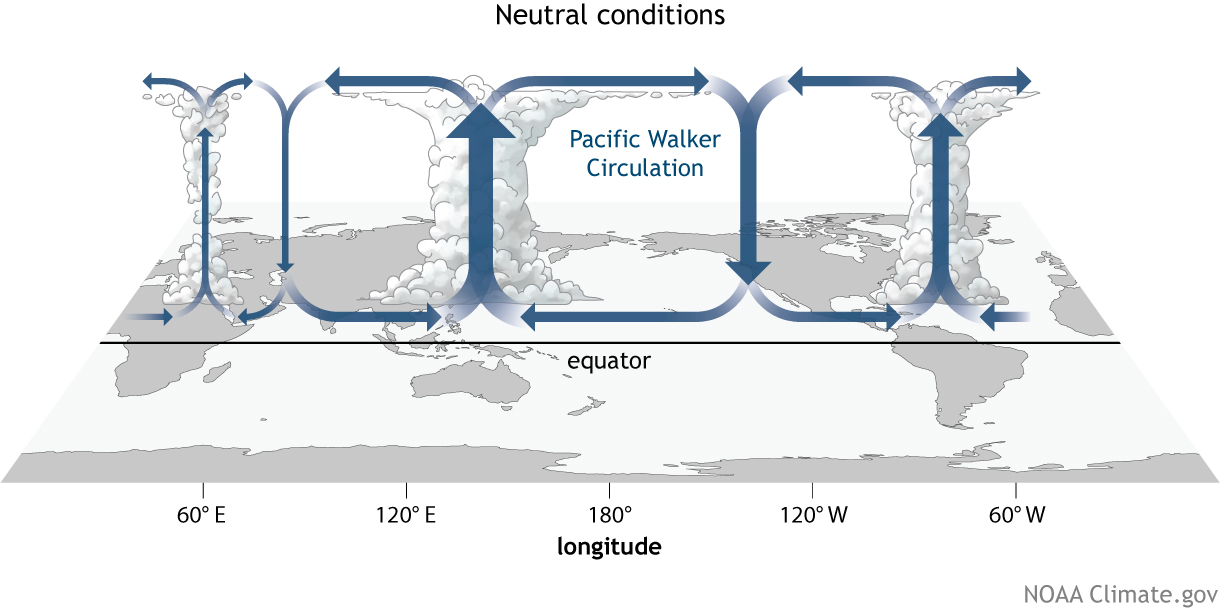
\includegraphics[width=\linewidth]{figures/Walker_Neutral_large.jpg}
\caption[The Walker circulation]{A schematic of the Walker circulation, depicting the mean zonal and vertical circulations, under neutral conditions of El Niño-Southern Oscillation. Schematic originally from: \url{www.climate.gov/}. }
\label{fig:walker_schematic}
\end{figure}
 
 
The Hadley cell is the meridional overturning circulation that arises from the differential heating between the tropics and the midlatitudes. This overturning cell is characterized by ascending motions in the tropics and descending motions in the subtropics, and acts to transport heat poleward from the equator \citep{lorenz1967}.  The ascending section of the Hadley circulation migrates meridionally with the seasonal cycle, the winter and summer cells interact with each other but also with the midlatitudes through eddy momentum fluxes \citep{bordoni2008monsoons}. 
The Hadley cell is not zonally symmetric; the boreal summer Hadley cell, for instance,  is primarily a result of ascent in the Indian Ocean and the west Pacific regions with a minor contribution from ascending motions in Central and North America \citep{hoskins2020}. 

The annual mean of solar radiation at the top of the atmosphere is roughly zonally distributed, however, the energy balance at the surface and the tropical circulation are not zonally symmetric. A prominent example of zonal asymmetry in the tropics is the Walker circulation. 
The Walker circulation is the zonal overturning circulation that is found in the equatorial Pacific Ocean, illustrated in Figure \ref{fig:walker_schematic} and characterized by ascending motion over the West Pacific and descending motions over the East Pacific\citep{walker1924,bjerknes1969,gill1980}. The dynamic and thermodynamic effects of the location and strength of convection associated with the Walker circulation have strong impacts across all the tropics and also the extratropics, known as teleconnections \citep{cai2019pantropical}.


The Inter-tropical Convergence Zone (ITCZ) is a tropical band of convective clouds and precipitation that migrates meridionally with the seasons \citep{schneider2014}. The ITCZ is arguably one of the most relevant features of tropical climate due to the strong influence on the low- and upper-level circulation associated with ITCZ, the high tropospheric heating due to deep moist convection in the ITCZ and the largest precipitation rates in the tropics are found in the ITCZ.
The ITCZ is characterized by a strong convergent flow in the low levels and a strong divergent flow at upper levels. 
The meridional migration of the ITCZ, as well as the mean latitude of the ITCZ, results from the energy and momentum balances so that the ITCZ is predominantly north of the equator because of the inter-hemispheric temperature contrast \citep{donohoe2013,bischoff2016}.



One of the phenomena of tropical climate that first generated interest in climate research is the monsoon \citep{halley}. The word \textit{monsoon} stems from the Arabic word for \textit{season} and is closely associated with the very first conceptions of a monsoon. 
The first widely accepted view of a monsoon was that the monsoon was the result of a large-scale land-sea breeze associated with the differential warming of the land and the ocean that force a seasonal reversal of the low-level winds that is also associated with the seasonal cycle of rainfall \citep{halley}. 

The traditional definition of the monsoon as a land-sea breeze is now known to present several shortcomings. Firstly, several mid-latitude regions would fit a monsoon definition based solely on a seasonal reversal of the wind \citep{gadgil2018}, and secondly, regions that are now recognized as a region with a monsoon climate, e.g. in South America, do not show a seasonal reversal of the winds, and the wind flow may just exhibit seasonal changes in direction and strength \citep{vera2006}. For these reasons, the land-sea breeze view of monsoons has recently been replaced by three alternative conceptions, an ITCZ-monsoon framework, a convective quasi-equilibrium interpretation and a moist static energy (MSE) zonal-mean energetic interpretation \citep{biasutti2018global,hill2019,geen2020}. 

\begin{figure}[b!]
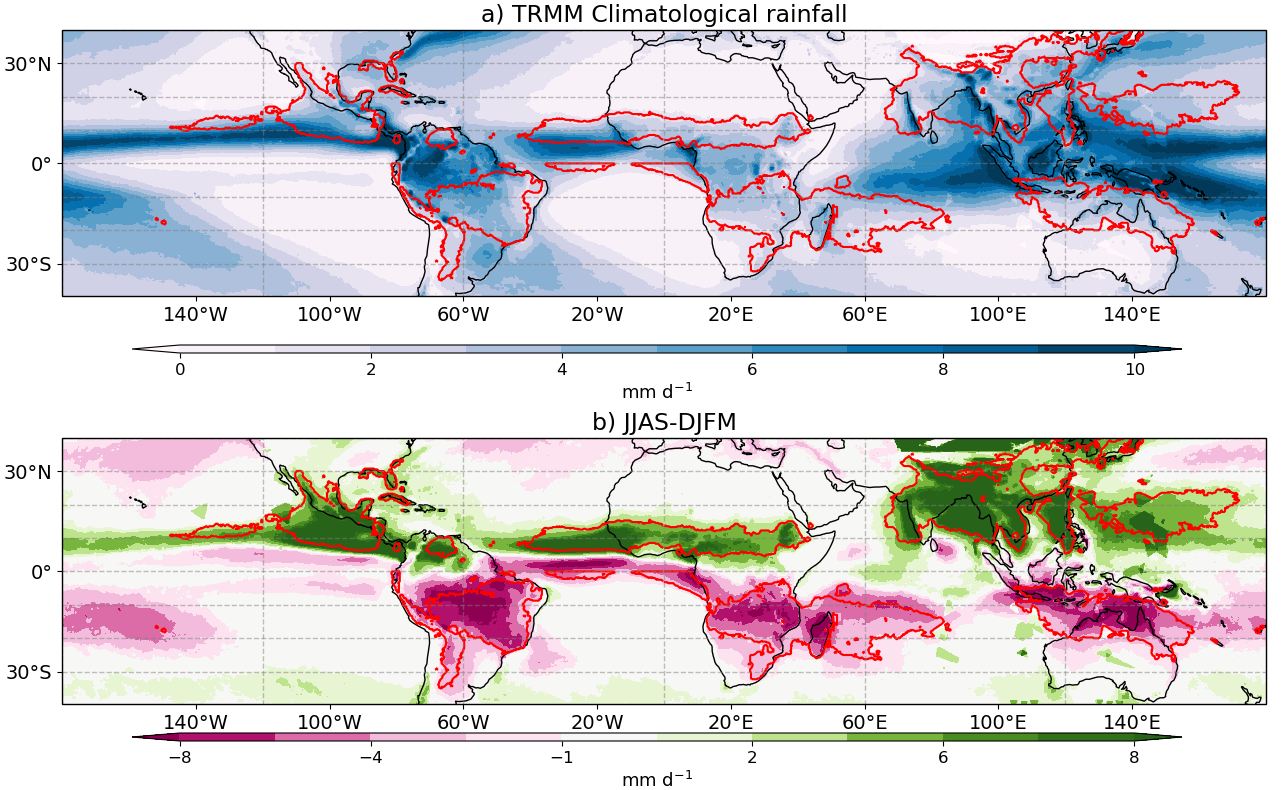
\includegraphics[width=\linewidth]{figures/trmmclima.png}
\caption[The global monsoon rainfall]{a) Climatological mean annual rainfall rates in the tropics using data from the Tropical Rainfall Measurement Mission (TRMM) dataset (1999-2018). b) The mean rainfall rate difference between boreal summer (JJAS) and austral summer (DJFM). The red contours highlight the regions where the mean summer rainfall amount accounts for more than 55\% of the mean total annual rainfall accumulation. }
\label{fig:monsoon}
\end{figure}


The first framework  explains monsoons as a poleward extension of the ITCZ into land  generalizing all monsoons as an expression of global tropical convergence resulting from the energy balance \citep{chao2001origin,gadgil2018}. This interpretation has led to the concept of \textit{the global monsoon}, a term that encompasses all the regions in the tropics that exhibit a strong seasonality in precipitation \citep{zhou2016,gadgil2018}. 
In practice, the global monsoon refers to those regions of the planet where more than 70\% of the total annual rainfall is observed during the local summer season, therefore, the concept of a global monsoon recognises the seasonality of precipitation as the key feature to diagnose a monsoon \citep{zhou2016,wang2017}.

Figure \ref{fig:monsoon} shows the global monsoon as depicted by the TRMM dataset. By this definition, the majority of the regions over land between 5 and 10 degrees away from the equator are part of the global monsoon.
A regional monsoon, such as the Indian Monsoon, is then a subset of the global monsoon with unique regional characteristics that shape this monsoon differently to other regional monsoons in terms of the seasonality, the strength and the dynamics. 
The American Monsoon System is then the regional monsoon that is located in the subtropics of North and South America. 


\cite{bordoni2008monsoons} provide an alternative conceptual view of monsoons, describing the characteristic rapid onset of a monsoon as a regime transition of the Hadley cell from an edddy-momentum  driven circulation, which resembles a canonical ITCZ regime, to a thermally direct circulation which resembles a monsoon-like circulation. The zonal mean MSE meridional gradient drives the ITCZ location and determines the strength of the overturning circulation by modulating the ventilation from midlatitude cooler and drier air in a feedback mechanism \citep{geen2020}. Even though this framework is posited as an axisymmetric framework, their predictions were broadly consistent with the Asian monsoon circulation. 


Convective quasi-equilibrium (CQE) is a theory for moist convection where convection sets the vertical temperature and moisture profiles to a convectively neutral state, thereby setting the free tropospheric temperature \citep{neelin2007moist}. For a monsoonal circulation, this theory emphasizes the coupling of convection and dynamics predicting that the subcloud layer equivalent potential temperature maxima must be collocated with the free tropospheric saturation equivalent potential temperature \citep{nie2010observational,geen2020}. The rapid onset of the Asian monsoon has been shown to be associated with the boundary layer moist entropy distribution, in agreement with predictions of CQE \citep{nie2010observational,boos2015review,ma2019}.

Several studies examine the monsoon as a large-scale phenomena through an axi-symmetric framework that assumes zonal symmetry investigated through global energetic diagnostics \citep[e.g.][]{faulk2017effects,geen2019,byrne2020}. The zonal-mean framework is common to the Hadley cell interpretation of monsoons \citep{bordoni2008monsoons}, as well as the ITCZ-monsoon theory. %This framework is very much in line with the global monsoon concept, that implies a zonally symmetric circulation driven by global energetic balance. 
However, regional monsoons are shaped by the asymmetries imposed by the orography, the characteristics of the surrounding ocean basins, land-sea contrasts and also the role of vegetation-hydrology coupling \citep{wang2017,pascale2019}. 
The importance of zonal asymmetries has raised multiple issues with large-scale so-called monsoon dynamics theories, as several predictions of these theories are not consistent with observations of regional monsoons \citep[e.g.][]{nie2010observational,smyth2018simulated,biasutti2018global,pascale2019}. 


The MSE budget and methodology is detailed in section \ref{sq:msemethod} but a broad description of the method and summary of results arising from the MSE budget applied to the monsoon phenomena is given below.
 The MSE budget framework suffers both from theoretical and practical shortcomings. One practical shortcoming is that the calculation of the budget terms post hoc in reanalysis or models results in very large residuals \citep{hill2019}, so these frameworks work best when the calculations of the budget terms are integrated online at each time-step \citep[e.g.][]{ma2019}.
The theoretical shortcoming is that the surface fluxes over land, e.g., in the Sonoran and Saharan deserts and the deep Amazon make the estimations of the roles of hydrology-vegetation feedbacks and their potential contributions to the MSE budget in observations very difficult to assess \citep{boos2016,pascale2019}. The use of simpler moisture budgets has proven useful in a regional monsoon context to investigate the sources of moisture for a monsoon in current  \citep{ordonez2019,martinez2019} and future climates \citep{smyth2020}, but this budget is mostly a tool and not a coherent theory for process-level understanding of monsoons.

Recent reviews acknowledge that all these frameworks have significant shortcomings when applied to regional local monsoons \citep{biasutti2018global,hill2019,geen2020}. These reviews conclude that a framework that reconciles the global energetic perspective with the characteristics of regional monsoons would be crucially important and very useful, but as several authors point out \citep[e.g.][]{biasutti2018global,hill2019}, also very hard to formulate. For example, the North and South American Monsoons depart from CQE, as precipitation does not follow the maxima in subcloud equivalent potential temperature \citep{nie2010observational,geen2020}. 

 
The Hadley cell interpretation of monsoons has significant shortcomings to depict some regional monsoons, particularly those that are not the Asian monsoon as the overturning circulation in the South Asian monsoon is strong enough to be represented by a clear thermally direct regime.
However, this energetic framework assumes no zonal transport of energy, which minimizes the role of orography and land-sea interaction \citep{biasutti2018global}.
One might reasonably infer from these results that the timing of transition in zonal mean overturning cells would be similar for monsoons at different longitudes but similar latitudes, which is not the case \citep{wang2017}.
Furthermore, a monsoon restricted to a small area, such as the North American and African monsoons may not show a clear zonally averaged overturning regime, and may be significantly affected by local shallow and deep circulations \citep{zhai2015regime}. For instance, \cite{smyth2018simulated} shows that the simulated West African monsoon when forced with different solar forcings exhibits a decoupling between the zonal-mean ITCZ location, the strength of the local Hadley cell and the monsoon rainfall, in opposition to the predictions of this framework \citep{bordoni2008monsoons}.


In short, despite significant progress in our understanding of the monsoon phenomena at the planetary-scale through zonal mean energetic frameworks, there is an important gap between large-scale theories of monsoon dynamics and the observed regional monsoons. 
The next section presents a summary of the American Monsoon literature, which explains the characteristics of these monsoons through the effect of regional features and dynamics, seemingly detached from the literature in this section.

\section{The American Monsoon System}\label{sq:bk_ams}

\begin{figure}[t!]
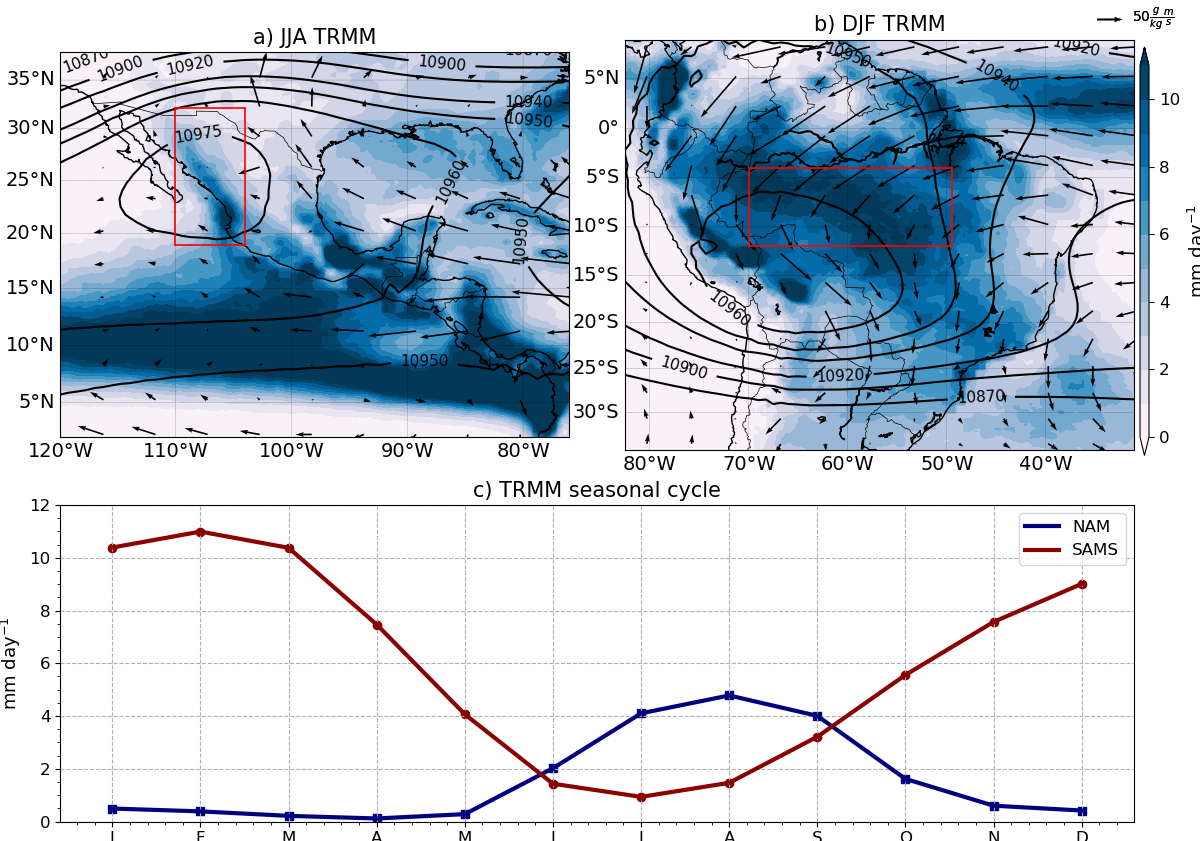
\includegraphics[width=\linewidth]{figures/amsclim.png}
\caption[The American monsoon system climatology]{ Climatological mean a) boreal and b) austral summer rainfall (shading), 850 hPa moisture flux (vectors) and geopotential height at 250 hPa (contours) in a) southern North America and b) South America. c) Monthly-mean seasonal march of precipitation in the TRMM dataset for two area-averaged time-series, the North American Monsoon (NAM) and the South American Monsoon System (SAMS) shown in the red rectangles in a-b). }
\label{fig:americanmonsoon}
\end{figure}

The American Monsoon System (AMS) is the main source of rainfall for tropical Latin America and is typically subdivided into the North and South American monsoon systems \citep{vera2006}. 
Although the spatial definition of the AMS is quite varied amongst studies, a general consensus is that the North American Monsoon is found in south-western North America (Figure \ref{fig:americanmonsoon}a) extending north from central-west Mexico into the southwestern United States and the South American Monsoon is centred in the deep Amazon south to the river mouth (Figure \ref{fig:americanmonsoon}b) \citep{adams1997,stensrud1997,vera2006}.


 The seasonal cycle of rainfall in the North American Monsoon is characterised by a wet July-August-September season and significantly drier conditions during the rest of the year \citep{adams1997} (Figure \ref{fig:americanmonsoon}c).
Three temporal stages describe the evolution of the North American Monsoon \citep{adams1997,geil2013}.
First, the onset stage (May-June) starts with a strong surface warming that leads to very high temperatures in the desert region.
Simultaneously, the sub-tropical jet weakens and migrates north decreasing the frequency of mid-latitude disturbances in the monsoon region \citep{douglas1993,turrent2009}.
These factors combine to develop a low-level thermal surface low pressure linked with an upper-level anticyclone and  moisture influx from the nearby Gulf of California and easternmost Pacific Ocean \citep{douglas1993,geil2013}.

Maturity (July-August) is the peak period of monsoon rainfall characterised by sustained deep convection \citep{barlow1998} and significant increases in low and mid-level moisture flux convergence and mid-level latent heating \citep{adams1997,cook2013}. This latent heating caused by deep convection can be diagnosed in the upper-level geopotential height (Figure \ref{fig:americanmonsoon}a) in the form of an anticyclone centred on the monsoon region. 
The moisture flux convergence decreases in August, after which precipitation recycling \citep{dominguez2008} plays an important role in keeping deep convection active until September.


 Decay (September-October) is the last stage of the monsoon, in many ways opposite to the onset stage, as is characterised by the equatorward migration of the sub-tropical jet \citep{higgins1997,geil2013}, evaporation in the nearby basins decreases and deep convection in the monsoon region gradually disappears \citep{douglas1993}.

 The origin of the high levels of moisture at low and midlevels in the monsoon region has been a matter of debate for a long time \citep{adams1997,barlow1998,vera2006,ordonez2019}.
A large number of studies aknowledge that the main source of moisture for the North American Monsoon is the East Pacific Ocean and to a second order, mid-level moisture advected from the Gulf of California can mix in the column \citep[e.g.][]{adams1997,stensrud1997,vera2006,turrent2009,ordonez2019}.
 %The high specific humidity in the mid-troposphere has been explained as the product of deep convection taking place on advected parcels from the EPO and GoC in combination with moisture mixing from the Gulf of Mexico \citep{douglas1993,stensrud1997,turrent2009}.

%A key aspect of this monsoon is the moisture advected by the low-level flow from the Gulf of California and the East Pacific Ocean and to a lesser extent the moisture mixed in the mid-troposphere from the Caribbean Sea and Gulf of Mexico \citep[e.g][]{stensrud1997,pascale2016,ordonez2019}.

The South American Monsoon System (SAMS) is a primary source of precipitation for South America, especially in the Amazon region \citep{gan2004,vera2006,jones2013}.
During austral summer (DJF), monsoon rainfall accounts for over 60\% of the total annual precipitation in the Amazon \citep{gan2004,marengo2012}, whereas
austral winter rainfall accounts for less than 5\% of the total annual rainfall \citep{vera2006}.
In the central Amazon, convective precipitation is observed from early October but the main rainy season extends from December to April \citep{machado2004,adams2013}, whereas convection in southeastern Brazil and Paraguay starts in November and peaks in January and February \citep{marengo2001,nieto2011}. 

A surface heat low appears in Bolivia in early austral summer, known as El Chaco Low, as a result of strong warming in austral spring \citep{marengo2012,sulca2018}.
 As this surface heat-low strengthens, low-level convergence drives the circulation into the low region.
 Simultaneously, an upper-level anti-cyclone (Fig. \ref{fig:americanmonsoon}b), known as the Bolivian High, develops in the same region as a signature of strong deep convection and latent heating \citep{marengo2001,vera2006}.

This low-level wind circulation importing moisture from the Atlantic is one of the most important features of the SAMS \citep{marengo2012,wang2017} as the flow modulates the moisture flux to the mainland and influences the ocurrence of active and break phases of the SAMS \citep{jones2002}, as well as changes in the temporal and spatial
distribution of rainfall \citep[e.g.][]{giannini2004,bombardi2011}.

As described in the previous sections, both the North and South American monsoon thermodynamics do not follow the CQE propositions, i.e., the maximum low-level moist static energy is not collocated with the maximum free tropospheric temperature. 
One possible reason for this is that the free-troposphere over southwestern North America is significantly drier than in other monsoon regions, decoupling the free troposphere from the boundary layer. One alternative hypothesis is that ventilation of low moist entropy air from the midlatitudes is responsible for this decoupling of the boundary layer and the free troposphere in the American monsoons \citep{boos2015review}.

%The SAMS and NAM did not fit the tradditional view of monsoons as the seasonal reversal of the winds was not as strong and clear as for other monsoons such as the Indian monsoon \citep{}. However, there is seasonal contrast in the zonal winds in both the NAM and SAMs as composite DJF-JJA wind differences suggest. 
%Furthermore, the NAM lower-level temperature structure departs from the quasi-equilibrium framework. A monsoon, can be described, through quasi-equilibrium arguments, \citep{}. %structures

\section{A review of the physical mechanisms for the Midsummer drought}\label{sq:litmsd}


The characteristics of the seasonal cycle of precipitation in northwestern Central America, the Caribbean and southern Mexico fit the definition of a monsoon climate \citep{wang2017} with a clear separation of the wet and dry seasons. 
However, this region shows a unique climatological precipitation feature. After monsoon onset, rainfall decreases considerably around the midsummer; this decrease is followed by a secondary increase in precipitation in the late summer \citep{mosino1966}, and for this reason this feature of the seasonal cycle is most commonly referred to in the literature as the Midsummer drought (MSD) \citep{magana1999}.   

 

The intraseasonal variations of precipitation associated with the MSD have been known for centuries and have shaped agricultural practices in the region. 
For example,  ancient Mayan texts suggest that agricultural rituals associated with the plea for rain-bearing clouds to the gods were significantly more frequent during the drier MSD period \citep{jobbova2018ritual}. In current days, the MSD is well known by local farmers who refer to the drier midsummer period as `El Veranillo' in Central America and `can\' icula' in southern Mexico because the drier period  coincides with the Canis Major constellation appearing in the sky \citep{dilley1996}.
% so that the MSD variations have shaped agricultural practices in the region for centuries.
%
% Save paragraph for onset method! 
%Farmers in Central America who are subject to climatic stress due to droughts, have already perceived and adapted to changes in the characteristics of the rainy season, such as the timing and strength of the midsummer drought \citep{hellin2017,de2018,harvey2018}, but it is unclear whether these perceived changes are a real trend in the observations \citep{anderson2019multiscale}. 

The two peak structure of the MSD has been diagnosed in the observed climatological precipitation of several regions of Mexico, El Salvador, Belize, Guatemala, Costa Rica and Cuba \citep[e.g.][]{mosino1966,magana1999,duranquesada2017,perdigon2018,martinez2019}.
However, notable differences in the seasonal cycle of precipitation have been found between mainland Central America and the Caribbean islands. The so-called first peak of precipitation occurs in June and the second peak in September in northern Central America whereas the two peaks are observed in May and October in the Caribbean.

\begin{figure}[t!]
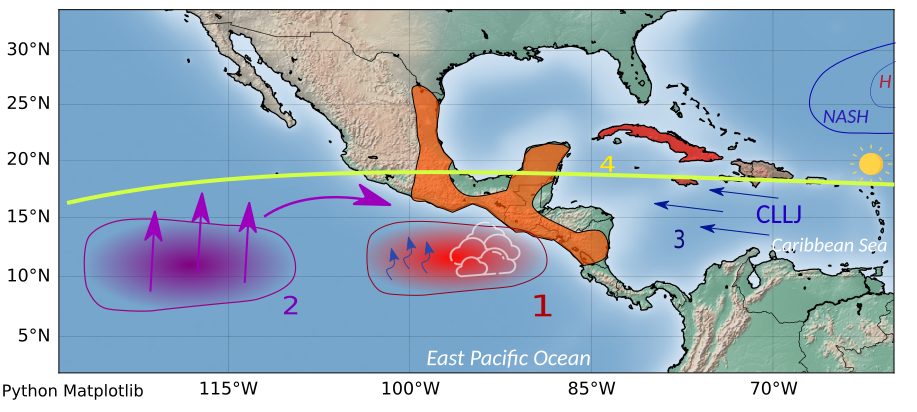
\includegraphics[width=\linewidth]{figures/back_msd_diag.png}
\caption[Mechanisms of the Midsummer drought]{A schematic of the Intra-Americas Seas region, depicting the four main mechanisms associated with the Midsummer drought in Mesoamerica (orange) and the Caribbean region (red). (1) The radiative-convective feedback mechanism associated with a double peak in East Pacific SSTs proposed by \cite{magana1999}. (2) The ascending region west of the continent produces an anomalous descending motion over the continent through a direct circulation, argues \cite{herrera2015}. (3) The Caribbean Low-Level Jet (CLLJ) modulates the moisture transport for all the region, with several studies supporting the hypothesis that seasonal cycle in the CLLJ is the main mechanism for seasonal fluctuations in rainfall \citep{duranquesada2017,martinez2019}. (4) The double-crossing of the solar declination angle, proposed by \cite{karnauskas2013}, suggests that each peak of precipitation is associated with peaks in the total shortwave radiation reaching the surface.  }
\label{fig:msd_schematic}
\end{figure}

%The mechanisms that cause the MSD have been debated since the first observational descriptions of the phenomenon \citep[e.g.][]{mosino1966}, as studies that aimed to explain the physical mechanisms MSD have not yet reached a consensus.
 In spite of extensive research to understand the physical mechanisms associated with the MSD   \citep[e.g.][]{magana1999,giannini2000,gamble2008,herrera2015,maldonado2017,straffon2019}, debate remains over which is the leading-order mechanism that causes rainfall to decrease at midsummer and increase again at the end of the summer.  % why rainfall increases again at the end of the summer, the end of the MSD, and why this happens at this time of the year. 
%Dynamical or thermodynamical mechanisms have been put forth and different roles have been proposed for the Atlantic and the East Pacific Oceans \citep[e.g.][]{magana2005,gamble2008,herrera2015}. 
Fundamental questions remain unclear such  as whether the MSD is caused by two precipitation enhancing mechanisms \citep{karnauskas2013} or a mechanism that inhibits rainfall at midsummer \citep{duranquesada2017}. 
Furthermore, the association between the MSD in Central America and in the Caribbean is still disputed \citep{gamble2008}, as most studies suggest that the two regimes are unrelated and therefore two different explanations are required to account for the two MSDs in these regions. 
Figure \ref{fig:msd_schematic} summarises the four main mechanisms that will be addressed in this section and in this thesis. 

%Any complete theory or conceptual model must account for the following characteristics of the seasonal cycle. First, the theory must explain the timing and strength of the first peak of rainfall. Second, the timing and strength of the MSD, i.e., what causes rainfall to decrease at midsummer. Finally, the theory must explain the timing and mechanism driving the second increase in precipitation after the midsummer. %The lack of a clear understanding of the processes that modulate the MSD makes climate change projections uncertain. 

One of the first hypotheses to account for the bi-modal distribution of rainfall was proposed by \cite{hastenrath1967} who argue that a double-crossing of the ITCZ can explain the MSD so that the first peak of precipitation is associated with early summer northward crossing of the ITCZ and the second peak the return or southward displacement of the ITCZ during late summer.
However, this theory fails to explain the MSD signal seen at latitudes as high as 29$^\circ$N \citep{perdigon2018,zhao2020}, a feature that will be shown in this thesis, which is further north than the northernmost extension of the ITCZ \citep{schneider2014}, and certainly the ITCZ does not cross twice so far from the equator. % \citep{magana1999,magana2005}.

\cite{magana1999} and \cite{magana2005} proposed a mechanism driven by radiative-convective feedbacks between the East Pacific (EP) sea-surface temperatures (SSTs) and deep tropical convective clouds (mechanism 1 in Figure \ref{fig:msd_schematic}). The coupling between the height and strength of convection, the incoming shortwave radiation and the SSTs are the key features of their framework. %Convection feedbacks with SSTs evaporation and
%moisture flux into the MSD region. 
The EP SSTs peak in May triggering large evaporative fluxes and deep convection in the EP ITCZ and the western coast of Central America.
The high convective clouds produce a radiative cooling effect at the surface due to a decreased incoming shortwave radiation associated with the reflectance of shortwave radiation by clouds.
This cooling  decreases SSTs and deep convective activity and thus accounts for the decrease of rainfall during midsummer.
The second peak in September is driven by an opposite mechanism, i.e., the decreased frequency of deep convective clouds during the MSD period in July and August reduces the cooling effect of the anvil clouds and increase the incoming shortwave radiation at the surface, SSTs and surface fluxes, all of which leads to an increase in precipitation during late August and September \citep{magana1999}.


%have been linked to several sources of seasonal variability,
%but debate is far from uncontroversial as to which is the principal mechanism to account for the MSD.
A large number of studies, in contrast, propose that the seasonal evolution of the North Atlantic Subtropical High (NASH) is the leading mechanism for the MSD \citep[e.g.][]{mapes2005,small2007,gamble2008,curtis2008,munoz2008,martinez2019,corrales2020}. The NASH is the subtropical anticyclone in the North Atlantic Ocean that migrates southwest during early boreal summer. The expansion and intensification of the NASH in boreal summer, according to these studies, strengthens the low-level trade winds, controlling the seasonal cycle of a low-level jet found in the core of the Caribbean Sea known as the Caribbean Low-Level Jet (CLLJ). 

The CLLJ is a key regional feature of the climate of the Caribbean and the Intra-Americas Sea  because the strength and direction of the flow in the Caribbean controls the underlying Caribbean SSTs and the regional moisture transport \citep{giannini2000,mestas2007,martinez2019,garcia2020sub}. 
 However, studies disagree on the specific roles that the CLLJ and the NASH play for the precipitation over the Mesoamerican region. 
 For example, some studies \citep[e.g.][]{giannini2000,mestas2007,gamble2008} suggest that  the expansion of the western flank of the NASH strengthens the CLLJ which cools the SSTs, through the effect of wind stress and mixed-layer mixing.
The cooling of SSTs diminishes evaporation and therefore low-level moisture which ultimately leads to less precipitation. In contrast, other studies propose that the seasonal cycle of the CLLJ (mechanism 3 in Figure \ref{fig:msd_schematic}) modulates seasonal variations of precipitation by modulating the regional moisture transport  \citep{small2007,munoz2008,herrera2015,duranquesada2017,martinez2019}. In this second hypothesis, the changes to the intensity of CLLJ influenced by the NASH modify the convergence and divergence patterns in the Intra-Americas Sea. In other words, the midsummer strengthening of the CLLJ increases moisture divergence, drying the atmospheric column over the Caribbean. 


%GCM literature needed.
 
    
%The strength of the easterlies crossing from the Caribbean Sea to the EP Ocean has been argued to modulate ascending and descending motions all across the Intra-Americas Seas region through the  effects of vertical wind shear and moisture divergence  \citep{herrera2015,corrales2020,zhao2020}. Moisture budgets over the Caribbean have diagnosed that changes to the regional and temporal distribution of moisture \citep{duranquesada2017,martinez2019,martinez2020} can influence the intra-seasonal and inter-annual variability of precipitation. % can be explained by the variability of the easterly wind flow in the CLLJ and the EP Ocean \citep{herrera2015,martinez2019,zhao2020}. 


%The strength of the flow crossing  between the EP Ocean and the Caribbean Sea has been argued to be a a function of the SST gradient across the basins, at least on interannual time-scales \citep{martinez2020}. This is particularly relevant as the Pacific Ocean is projected to warm more than the Caribbean Sea in future decades, which could change the SST gradient, strengthen the CLLJ and shift the regional precipitation patterns \citep{corrales2020}.
    
 \cite{herrera2015} shows that during the drier months in Central America in the Midsummer, convective activity west of the central American continent gets stronger with heavier precipitation (mechanism 2 in Figure \ref{fig:msd_schematic}).  Their evidence suggests that the gap flow that originated from the CLLJ in the Caribbean Sea controls the location of ascending and descending motions, and the MSD may be explained by the seasonal variations of the coupling of the low-level wind flow with the underlying EP SSTs.
\cite{herrera2015} further argued that the exit region of the CLLJ is located to the east of the region of the strongest MSD signal, which suggests that the moisture divergence effect over the central American MSD is minimal. 



A different mechanism, proposed by \cite{karnauskas2013}, argues that the biannual crossing of the solar declination angle can control precipitation and explains the bimodal characteristics of the seasonal cycle (mechanism 4 in Figure \ref{fig:msd_schematic}). In this mechanism, the MSD is driven by two precipitation enhancing periods that are separated by a relatively normal, and drier, period. This theory differs from those previously discussed which explained the MSD through mechanisms that inhibit convective activity in the midsummer whereas \cite{karnauskas2013} argues that the solar declination angle that crosses twice through Central America, once during June and a second time during September, increases convective activity during each crossing. 

The variations of incoming shortwave radiation associated with the declination angle modulate the SSTs, surface fluxes and therefore convective activity. In other words, the first crossing of the solar declination angle increases the incoming shortwave radiation which increases the SSTs, evaporation and leads to a peak of precipitation, i.e., the first peak. After the shortwave radiation is reduced the MSD period appears. The second crossing of the solar declination angle, similarly, explains the second peak as the second increase in incoming shortwave promotes more deep convection than during the MSD. 



Other mechanisms have been proposed arguing that the MSD is a result of vertical wind shear affecting convective instability or the Saharan dust controlling  the microphysics of clouds \citep{angeles2010origins}.
For instance, \cite{perdigon2019} also finds a link between the frequency and spatial distribution of the first peak rainfall rates and the Madden-Julian Oscillation. 

\section{El Niño Southern Oscillation: impacts to the American monsoon system}
\label{sub:lit_enso}



 El Niño-Southern Oscillation (ENSO) is a phenomena that primarily affects the local ocean and atmosphere of the equatorial Pacific Ocean, but these changes are profoundly important for the global climate system, which is why ENSO is commonly known as the leading mode of interannual variability. 
 The term \textit{'El Niño'} was initially coined by Spanish colonizers when they learnt from Peruvian fishermen that the ocean surface temperatures in the easternmonst Pacific Ocean increased notably in some years around December time. 
 For religious reasons, the colonizers termed the SST increase as Christ Child -- \textit{El Niño}. 
 %The effect teleconnections can be felt in the tropics through changes in the tropical overturning circulation but also impacting extratropical circulations and thus ENSO impacts extend to most regions on the planet.
 
 
 
  Later on, sir Gilbert \cite{walker1924} coined the term \textit{Southern Oscillation} to describe the synchronous changes to the sea-level pressure of the Indo-Pacific region and South America. 
  \cite{walker1924} and \cite{walker1932} are the first analyses of synchronous effects of the tropical circulation over local precipitation, temperature and pressure. Further research \citep[e.g.][]{troup1965} would highlight that these remote changes in pressure were driven by the east-west pressure gradient in the equatorial Pacific. 
  
  The changes in the pressure field associated with the Southern Oscillation (SO) are now part of what is known as the Walker circulation, which intertwines the dynamics of the zonal circulation in the East Pacific with the SSTs over the underlying ocean. ENSO is then characterized as a coupled phenomena composed of an oceanic part, \textit{El Niño}, and an atmospheric component associated with the zonal circulation but best characterized by changes to the surface pressure field, the Southern Oscillation. 
  
  
% The SO changes are intertwined with changes to the Walker circulation as the surface pressure variations affect the strength of low-level trade winds, which are a big component of the Walker circulation. In other words,   ENSO is the coupled ocean-atmosphere oscillation of the equatorial Pacific sea-surface temperatures (SSTs) and the atmospheric pressure and wind fields, particularly those associated with the Walker circulation\citep{wang2004}. %; these variations in the SO are typically described as with the Walker circulation. %changes and the Southern Oscillation (SO) is associated with changes in the zonal gradient of MSLP. Combined, El Niño and the SO compose the ENSO phenomenon.
  
\begin{figure}[t!]
\centering
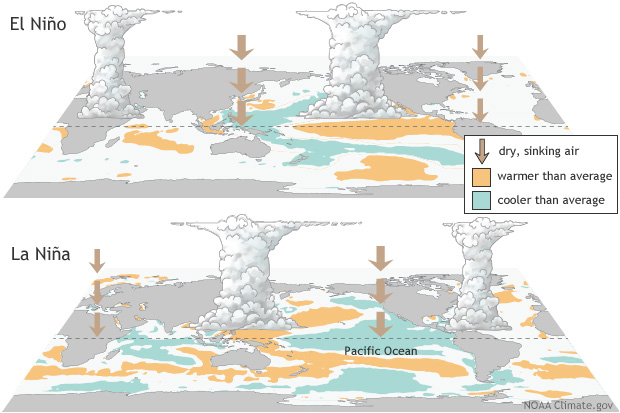
\includegraphics[width=\linewidth]{figures/ENSO}
\caption[El Niño Southern Oscillation and the Walker circulation]{Schematic of the positive (upper) and negative (lower) phases of ENSO. Regions with tall clouds indicate more ascent and convection than normal whereas brown arrrows indicate dry descending air. Obtained from the National Oceanic and Atmospheric Administration at \url{https://www.climate.gov/enso}. }
\label{fig:enso}
\end{figure}  
 ENSO has several unique features, such as no robust periodicity as events may occur every 2 to 7 years and a seasonal phase-locking that are associated with ENSO events peaking in boreal winter in observations \citep{wang2004}. Even though the underlying physics that cause ENSO and explain the variability in the periodicity of the phenomena is still debated \citep{wang2004,christensen2017}, several aspects are now better understood. 
For example, the local effect that ENSO events have over on the location and strength of deep convection in the equatorial Pacific have long been thoroughly described \citep{trenberth1997,neelin1998}. 

During a neutral state of ENSO, the Walker circulation is found in the climatological state, with ascent and wet conditions in the West Pacific  and descent and drier conditions in the East Pacific. During El Niño the Walker circulation and low-level trade winds weaken which is associated with an eastward shift of deep convection along the equatorial Pacific (Figure \ref{fig:enso}), with convective rainfall becoming more frequent in the central and even eastern Pacific than normal \citep{neelin1998,wang2004}. During La Niña the opposite happens and the Walker circulation stregnthens which leads to stronger convection in the West Pacific and stronger ascent on the East Pacific (Figure \ref{fig:enso}). 


In other words, ENSO imposes a strong control on the location and strength of the Walker circulation (Figure \ref{fig:enso}). These changes to the strength and position of the convective regions in the Pacific Ocean can then propagate to other regions of the planet; these far-distant effects are commonly known as \textit{teleconnections}.  
For example, ENSO has a direct effect over other tropical regions outside of the Pacific through the Walker circulation, see Figure \ref{fig:enso}, as upper-level wind anomalies induce anomalous vertical motions over the monsoons in West Africa \citep{ropelewski1986,ropelewski1987} or South America \citep{sulca2018}.  
  Other mechanisms of ENSO teleconnections to higher latitudes include changes to the position and strength of sub-tropical jets \citep{fereday2020}, changes to the Pacific and North American circulation patterns \citep{bayr2019} as well as impacts to the North Atlantic via the stratospheric polar vortex \citep{domeisen2019}.
  
  In South America, the effects of ENSO are felt throughout the continent and throughout economic sectors from Peruvian fishermen \citep{takahashi2004} to the Amazon rain-forest and the plainlands in South-eastern South America \citep{grimm2011,marengo2012}. 
  One key aspect of current research on ENSO impacts to South America is the observed non-linearity and non-symmetry in the teleconnections, which has mainly been attributed to ENSO diversity \citep{tedeschi2015,cai2020}.
A non-linear teleconnection refers to a non-linear scaling between the strength of an ENSO event, typically measured by an SST index, and the magnitude of the response, in most cases precipitation response. %So two observed ENSO events, although very similar in magnitude may show different strengths and even patterns in these teleconnections \citep{}. 

Observations have shown that the maximum SST anomaly does not always appear in the same region of the Pacific Ocean \citep{ashok2009,dommenget2013}. These differences in the SST patterns are referred to as ENSO \textit{ diversity} or \textit{flavours} which can be broadly summarized as two flavours for each phase. The flavours or types of event are defined based on the location of the SST anomaly so the most common division is into Central and Eastern Pacific events.  In observations, each type of event is usually also associated with the strength of the event \citep{dommenget2013}, with eastern Pacific events being usually stronger than Central Pacific events. 

The strength and patterns of ENSO teleconnections to the SAMS have been shown to depend on the type of event  \citep{rodrigues2011,sulca2018}. 
\cite{cai2020} provides a recent review on the differences in the impacts that Central and Eastern Pacific (CP and EP) events have on South American precipitation and climate features.
The observed record shows that the teleconnections affecting the Amazon and northeastern Brazil are most pronounced during EP El Niño events and CP La Niña events than the CP El Niño events and EP La Niña events. 
 This recent review also highlights the need for further modelling work to test observation-driven hypothesis, as the observed record is too short to make confident statements about the mechanisms associated with ENSO teleconnections.

%ENSO has motivated extensive research using GCMs to understand the mechanisms related the origin of ENSO \citep{christensen2017}, the feedbacks and processes that phase-lock the phenomena \citep{neelin1998}, as well as how will ENSO characteristics change in the future \citep{cai2015a,santoso2017}.


 
 
 


%The period of ENSO of 2-7 years \citep{neelin1998,wang2004} was poorly represented in CMIP3 and CMIP5 models \citep{guilyardi2009}, particularly by models that had much stronger power spectrums than the observed.



\section{Stratosphere-Troposphere Coupling in the Tropics}\label{sq:qbolit}

%\begin{figure}
%\centering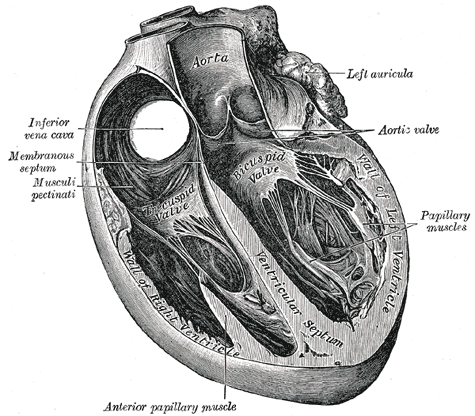
\includegraphics[width=0.7\textwidth]{figures/sample/Gray498.png} 
%\caption[Four-chamber illustration of the human heart.]{Four-chamber illustration of the human heart.  Clockwise from upper-left: right atrium, left atrium, left ventricle, right ventricle.}
%\label{fig:fourchamber}\end{figure}
The troposphere is the lowermost layer of the atmosphere ranging from the surface up to 10-15 km where the vertical temperature profile is characterized by a decrease of temperature with height so that convective instability plays an important role for vertical motions.
The layer above the troposphere is called the \textit{stratosphere} where the vertical temperature gradient is reversed and temperatures increase with height so that the atmosphere is stable to upward motions, this layer and spans from 10-20 km up to 50 km in altitude \citep{andrews1987}. 
The transition layer in between the troposphere and the stratosphere is referred to as the tropopause, which is a transition region where the vertical temperature gradient reverses and the atmosphere is stable to upward motions. 

%The chemistry and dynamics of the stratosphere are very different from the troposphere both in temporal and spatial scales. The stratosphere is generally drier and well-mixed so that local ultraviolet absorption and infrared radiative loss exert the largest influence over the seasonal cycle of temperature and zonal winds in this layer \citep{andrews1987}.
%The strength of the inversion layer of the tropopause prevents ascending tropospheric parcels from entering the stratosphere. However, the tropopshere and stratosphere do communicate and exchange momentum and mass through waves, intrusions and radiation. 
% These exchanges typically include the tropopause. exists between stratosphere and troposphere. 

Stratosphere-troposphere coupling refers to events or processes where the two layers are notably affected by each other so that the temperature or wind flow of the two layers vary together, or \textit{couple}. One prominent example of this coupling is the effect of the stratospheric polar vortices over the zonal flow in the troposphere \citep{thompson2005,domeisen2019}. 
However, semi-periodic climatic variability in either layer can also have effects over the other layer. The dominant mode of interannual variability in the equatorial stratosphere is such an example and is introduced in the following section. 

% in the  Generally, stratospheric processes are slower and can communicate to the other latitudes of the stratosphere with more impact than tropospheric processes where friction and other processes reduce the memory of the lowermost layer. 
%Typically, the communication between the troposphere and the stratosphere occurs from the bottom layer upwards. 
%However, evidence of communication in both directions, or coupling, has been found at low latitudes and in the midlatitudes. 

\subsection{The Quasi-biennial oscillation (QBO)}

The stratospheric quasi-biennial oscillation (QBO) was discovered 60 years ago through balloon observations  that revealed that the zonal winds reverse direction in a semi-periodic way with accompanying temperature variations \citep{ebdon1960,reed1964}. The QBO has then been characterized by further observations as alternating easterly and westerly wind regimes associated with a descending zonal wind shear from up to 50 km down to 10 km, with a mean oscillatory period of 28 months \citep{baldwin2001}. 
The downward propagation of the easterly and westerly wind regimes, amplitude and the mean period have been explained by the interaction of a broad spectrum of gravity and Kelvin waves of tropospheric origin with the equatorial stratospheric zonal mean flow  \citep{baldwin2001}.

The wind variation in the middle stratosphere associated with the QBO are greater than the seasonal cycle \citep{andrews1987} and this vertical wind shear imposes a temperature signal through the thermal wind relationship, which can be expressed as: 

\begin{equation}
\frac{\partial{u}}{\partial{z}}=\frac{-R}{H \beta}\frac{\partial^2 T}{\partial y^2}, 
\end{equation}

\noindent where $\partial u / \partial z$ is the vertical shear of the zonal wind, $R$ is the ideal gas constant, $y$ is the latitude, $H$ is a scale height of the atmosphere (7-8 km) and $\beta$ is the first derivative of the Coriolis term in the meridional coordinate $y$. 

In order to maintain thermal wind a westerly (easterly) vertical shear requires a latitudinal temperature gradient with a warm (cold) temperature anomaly over the equator. These temperature anomalies are achieved through an induced mean meridional circulation, often referred to as the secondary circulation of the QBO \citep{plumb1982,li1995,baldwin2001,ribera2004}. This anomalous circulation is characterized by reduced upwelling during westerly shear phases and increased upwelling during the easterly phase. These meridional circulation perturbations adiabatically warm (anomalous descent at the equator) and cool (anomalous ascent) for westerly and easterly shears, respectively, at the equator. 

These induced meridional circulations also give rise to an ozone anomaly, with positive (negative) ozone anomalies associated with a descending wester (easterly) QBO phase, which further enhances the temperature anomalies.
The temperature anomaly driven by the meridional circulations impact the height and temperature of the tropopause in the tropics \citep{baldwin2001,tegtmeier2020,tegtmeier2020b}. 
The easterly phase of the QBO (QBOE) is associated with a higher and colder tropopause in the tropics whereas the westerly phase (QBOW) is observed with lower and warmer tropical tropopause \citep{tegtmeier2020}. These variations in the tropopause characteristics, amongst other effects associated with the QBO, have been hypothesized to affect, to different extents, a range of tropical phenomena, and in particular, deep convective systems. % such as the height and temperature of the tropopause\citep{tegtmeier2020b}. 

The combination of dynamic and thermodynamic effects of the QBO in the equatorial stratosphere are associated with long-distance impacts across the stratosphere \citep{holton1980,lu2020} and down to the surface \citep{garfinkel2010,gray2018}. The most well-known teleconnection of the QBO is with the polar stratosphere, in particular, how the direction of the zonal mean flow in the equatorial stratosphere modulates the propagation of extratropical waves and therefore also influences the wintertime stratopsheric polar vortex \citep{lu2020}, which can have profound impacts over the surface in polar and midlatitude regions.



\subsection{Tropical teleconnections of the QBO}\label{sq:trop_qbo}



 The influence of the QBO on the dynamic and thermodynamic characteristics of the tropical upper-troposphere-lower stratosphere  (UTLS) region has raised interest in possible indirect effects of the QBO over tropical deep convection and clouds.
\cite{gray1984} was amongst the first to suggest an influence of the QBO over tropical systems, in particular, that Atlantic tropical cyclone activity was enhanced during QBOW compared to QBOE. 
\cite{gray1992} further argued that the anomalous vertical wind shear in the UTLS associated with the QBO affects the strength of convection in monsoonal and convergence zones to the extent that the vertical wind shear can modify ENSO frequency. Their results suggest that El Niño events are favoured during QBOE and  La Niña events are more frequent during QBOW.

The evidence by \cite{gray1992} has motivated further observational and modelling research on QBO tropical teleconnections; some of this research has contested Gray's results \citep[e.g.][]{chan1995,camargo2010,hansen2016tropospheric}. 
For example, \cite{giorgetta1999} was amongst the first to use a global climate model (ECHAM4) to investigate the effects of the QBO over tropical convection. \cite{giorgetta1999} focused on the role that the QBO plays in modulating the strength of the East Asian and Indian monsoons. Their findings suggest that monsoon variability was partially modulated by the QBO, with strong effects over the properties of clouds at 100 hPa. \cite{giorgetta1999} argues that these differences could be explained by the effect of the QBO on the UTLS static stability and a consequent effect over the vertical extent of deep tropical convection. 

\begin{figure}[t!]
\centering
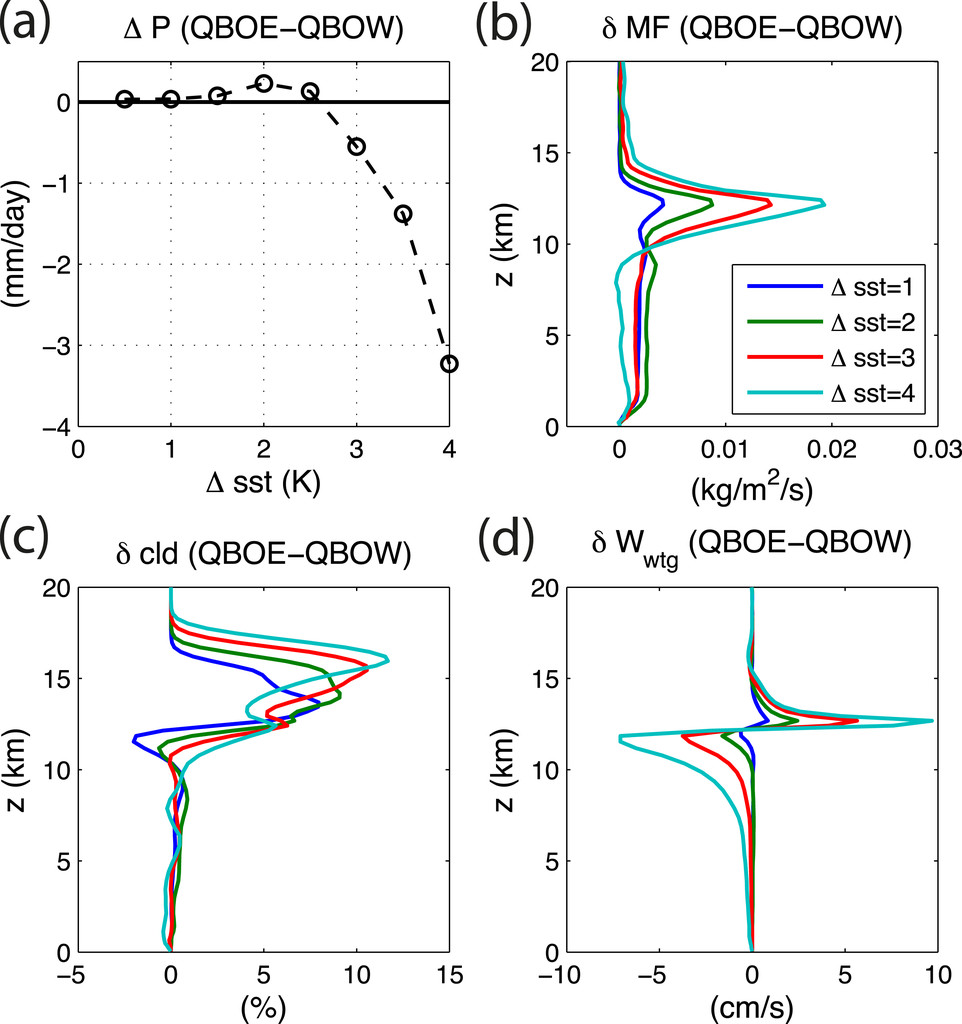
\includegraphics[width=0.85\linewidth]{figures/nie_sobel}
\caption[The non-linear relationship of the QBO with SST forcings]{(a) QBO anomalous precipitation as a function of SST forcing. The $\delta sst$ are increments over a baseline of 301 K throughout the whole model domain. (b)–(d) The differences of mass flux in cloud cores, cloud fraction, and the parametrized large-scale vertical velocity derived from the weak temperature gradient approximation, respectively, between experiments with the QBOE and QBOW temperature profiles. Figure 3 from \cite{nie2015}. }
\label{fig:nie}
\end{figure}  

Further modelling work has been carried out, for instance by \cite{garfinkel2010} and \cite{garfinkel2011} that used the Whole Atmosphere Community Climate Model (WACCM) to understand the effect of the QBO over tropical precipitation, the subtropical jets and the wintertime polar vortex. \cite{garfinkel2010} shows that the canonical ENSO teleconnections to the North Pacific are stronger during QBOW in WACCM and reanalysis suggesting that the QBO modulates the wave propagation activity associated with ENSO events.
 \cite{garfinkel2011} uses perpetual winter conditions in the WACCM model to show that the QBO modifies the upper-tropospheric zonal wind at the equator and the strength and location of subtropical jets, particularly at their exit region, as the subtropical jet is weakened during QBOE conditions.

 The response of convection to the UTLS temperature anomalies associated with the QBO was investigated in cloud-resolving model simulations by \cite{nie2015}. Their experimental design used the System for Atmospheric Modelling (SAM), varying SST boundary conditions with increments over a baseline SST level of 301 K, the use of the weak-temperature gradient (WTG) \footnote{The weak temperature gradient approximation makes use of the relatively small horizontal gradients of temperature and density in the tropics, which simplifies some of the primitive equations and has allowed several numerical analyses of tropical dynamics using simplified models \citep{sobel2001wtg}.} approximation and an idealized vertical temperature profile to simulate the effect of the QBO temperature signal. 
 Figure \ref{fig:nie} shows that the precipitation differences between QBO phases depend on the SST forcing.   The precipitation difference between QBO temperature anomalies is positive under relatively small SST anomalies but in experiments with large SST anomalies this difference becomes negative and overall larger than under small SSTs. The difference in mass flux and cloud fraction is also sensitive to the underlying SSTs, as increased mass flux during QBOE is increased for larger SSTs.  In other words, the QBO influence on precipitation is non monotonic and largely depends on the underlying SST field.
 
%  The cloud fraction in the upper troposphere is increased during QBOE compared to QBOW whereas the ascending motions show peculiar behaviour with stronger ascent above 12 km for QBOE and weaker ascent below 12 km. 
  The results of \cite{nie2015} suggest that the QBO influences convection in two ways that are non-linear and the authors argue are the result of competing mechanisms. Their argument is that since  the mass flux in the upper troposphere is increased during QBOE but there is also an increase in gross moist static stability (GMS) the result is an increase in the efficiency of large-scale vertical motions during QBOE for large SSTs, which acts to reduce precipitation.  Secondly, the QBO modifies the fraction of high-level clouds resulting from deep convection which modifies the radiative heating to the column which increases precipitation during QBOE.  Figure \ref{fig:nie}a then shows how these competing effects change for different SSTs with the gross moist stability mechanism dominating for large SSTs.

Various attempts have been made to determine a relationship between the QBO and deep convection in observations. 
One influential study by \cite{collimore2003} analysed satellite-derived out-going long-wave radiation (OLR) in the tropics composited by QBO phase. These composites suggest that OLR is significantly different between QBO phases in most monsoon regions, such as Central America  and the West Pacific, with an overall indication that convective activity is reduced during QBOW compared to QBOE. This influence, however, was not found to be zonally symmetric and in fact the longitudinal variations of the QBO-related OLR differences were suggestive enough that \cite{collimore2003} argue for a possible role for the QBO to modulate the Walker circulation, which would explain the lack of zonal symmetry in their results. 


Another relevant study by \cite{liess2012} found that satellite-derived cloud thickness and frequency  and upper-level velocity potential had a significant and longitudinally asymmetric response to the QBO. In particular, their results show increased convective activity during QBOE in the West Pacific but the opposite for the East Pacific.  For this reason, \cite{liess2012} also argue that the strength of the tropical overturning circulation may be modulated by the QBO, indicating the possible role of both the vertical wind shear and the upper-level static stability to modulate deep convection. 


The topic of QBO tropical teleconnections has regained attention due to recent findings suggesting a link between the QBO and the Madden-Julian Oscillation (MJO) \citep{son2017} which motivated extensive research \citep[see e.g.][]{lee2018,wang2019,martin2020jgr} due to the worldwide impact of the MJO.
 The MJO in observations shows a stronger amplitude and more predictability during QBOE, but further inspection in cloud-permitting and forecast models have not provided conclusive answers to this puzzle \citep{martin2019,martin2020jgr}. 
 
 Questions still arise as to whether this tropical link is real or due to chance, for instance \cite{wang2019} argued that the increased predictability of the MJO under the QBOE phase is included in the initial conditions, and thus not a result of a mechanistic effect of the QBO on the MJO. More generally, whether the QBO has a considerable effect on deep convection in general is debated as several plausible mechanisms exist in the literature \citep[see e.g.][]{nie2015} such as the effect of wind shear, the tropopause height, the cold-point temperature, static stability and/or feedbacks with very high cirrus and cumulunimbus clouds. 

%The use of climate models to understand these tropical teleconnections of the QBO has proven difficult due to biases in both the MJO and the QBO representations. State-of-the-art CMIP6 models struggle to reproduce several of the characteristics of the QBO \citep{richter2020}. For instance,  weaker temperature QBO signals in the lowermost tropical stratosphere in the models, e.g., compare the QBOE-W difference plot in Figure \ref{fig:qbo}. The weaker temperature signal may be key for possible biases in the tropical QBO links discussed above, such as the the QBO-MJO link which is missing from CMIP6 models \citep{kim2020} and from seasonal prediction forecast models \citep{wang2019,martin2020jgr}. 
%\begin{savequote}[8cm]
%\textlatin{Neque porro quisquam est qui dolorem ipsum quia dolor sit amet, consectetur, adipisci velit...}

%There is no one who loves pain itself, who seeks after it and wants to have it, simply because it is pain...
 % \qauthor{--- Cicero's \textit{de Finibus Bonorum et Malorum}}
%\end{savequote}

\chapter{\label{ch:1-intro}Data and methods} 

\label{sq:data}

\minitoc



\begin{sidewaystable}%[t!]
\small
\caption{Summary of the datasets used in this study. For each dataset, the acronym used hereafter, the period of coverage, the field used and the horizontal resolution are shown. Some datasets extend further back in time, but only the satellite-era period is used in most of the datasets.
The variables used are: precipitation, surface-air temperature ($2mT$), sea-level pressure (SLP), SSTs, the x and y components of the wind ($u$, $v$), the lagrangian tendency of air pressure ($\omega$), outgoing longwave radiation (OLR), geopotential height (GPH) and specific humidity ($q$).}
\begin{tabular}{p{5cm}|p{1.47cm}p{3.45cm}p{2.12cm}p{4.2cm}p{2.12cm}p{3.54cm}} \label{tab:1}
\textit{Dataset/ Version}                    & \textit{Acronym} & \textit{Variable} & \textit{Period} & \textit{Data type}             & \textit{Resolution} & \textit{Reference}                 \\ \hline \hline
Global Precipitation Climatology Project v2.3 & GPCP       & Precipitation       &   (1979-2018)       &  Surface and satellite & 2.5$^\circ$x2.5$^\circ$  & \citep{adler2003}               \\
 Global Precipitation Climatology Centre    & GPCC          & Precipitation       & (1940-2013)       &  Surface station                 &  0.5$^\circ$x0.5$^\circ$ & \citep{becker2011}              \\
Climate Prediction Center Merged Analysis of Precipitation & CMAP      & Precipitation       &   (1979-2016)       & Satellite calibrated with surface rain-gauge & 2.5x2.5$^\circ$  & \citep{xie1997}     \\
Climatic Research Unit TS  v4.     & CRU4         & Surface temperature  & (1979-2017)       &  Surface station    &  0.5$^\circ$x0.5$^\circ$   &        \citep{harris2014}                            \\
  Climate Hazards Infrared Precipitation with Stations   & CHIRPS          & Precipitation       & (1981-2018)       &  Surface rain-gauge and satellite               &  0.05$^\circ$x0.05$^\circ$ & \citep{funk2015}              \\
% Global Precipitation Climatology Centre    & GPCC          & Precipitation       & (1891-2013)       &  Surface station                 &  0.5x0.5$^\circ$ & \citep{becker2011}              \\
Tropical Rainfall Measurement Mission 3B42 V7       & TRMM          & Precipitation       & (1999-2018)   & Satellite calibrated with surface station   & 0.25$^\circ$x0.25$^\circ$  &  \citep{mission2011} \\
Hadley Centre SST3                           & HadSST          & SST               & (1940-2018)   & Buoy and satellite              & 2.5$^\circ$x2.5$^\circ$  &  \citep{kennedy2011} \\
European Centre for Medium-Range Forecasting ERA-5                            & ERA-5             & $2mT$, SLP, $u$, $v$, $\omega$, OLR, $q$, SST, GPH, precipitation    &  (1979-2018)    &  Reanalysis       & 0.75x0.75$^\circ$ &  \citep{era5,era5hersbach}
\end{tabular}

\end{sidewaystable}
\section{Observations and reanalysis data}
%We use several observational and reanalysis datasets to validate the simulations.
Table \ref{tab:1} summarises relevant information of the observations and reanalysis datasets used in this study.
In short, surface and satellite observations were used where available, whereas other metrics were taken from reanalysis data from the
European Centre for Medium-Range Weather Forecasts (ECMWF): ERA-5, downloaded from \url{https://climate.copernicus.eu/climate-reanalysis}.
Four different precipitation datasets are used. 

The Tropical Rainfall Measurement Mission (TRMM) dataset is a multi-satellite multi-sensor product that in some versions is calibrated with gauge analyses \citep{huffman2007}. A set of microwave sensors onboard low earth orbit (LEO) satellites, such as the Microwave Imager (TMI) and the Advanced Microwave Scanning Radiometer-Earth Observing System (AMSR-E), provide the main source of information about hydrometeors for TRMM. However, even using the products of several satellites there is a sparse sampling of time-space precipitation  in passive microwave techniques. Therefore, this data is complimented by infrared measurements onboard geosynchronous earth orbit satellites. Other sources of information include a radar onboard TRMM and rain gauge analysis. Details of the research product can be found in \cite{huffman2007} and \cite{mission2011}.

The Climate Prediction Center Merged Analysis of Precipitation (CMAP) dataset is a global merged product of satellite and ground based observations but also constrained by a numerical model \citep{Xie2007}. This dataset was first produced at monthly-mean resolution \citep{xie1997} but is now available as a collection of products at several temporal scales. The pentad-scale version of CMAP is used in this study. % and is used in this study at the pentad-mean scale. 

The Climate Hazards Infrared Precipitation with Stations (CHIRPS) is relatively more recent merged product. This dataset uses high-resolution rain-gauge station data that is complimented by satellite cloud cold duration estimates on regions where station data is sparse. The products are calibrated with TRMM data \citep{funk2015}, so they are cannot be considered an independent source of information from TRMM.

The TRMM dataset has a high horizontal and temporal resolution and was used in several CMIP assessments \citep{geil2013,jones2013} as a reliable source of precipitation \citep{carvalho2012}. Therefore, we use TRMM as our best estimate for the spatial and temporal characteristics of the AMS rainfall. However,
 the period covered by TRMM (1998-2018) is too short to analyse statistically robust teleconnections or variability, so we use GPCP, GPCC and CHIRPS for their longer period. Although a thorough validation and comparison of these datasets across the AMS domain is missing, several studies have analysed  one or more of these datasets in regions of the AMS \citep[e.g.][]{franchito2009,dinku2010,trejo2016}.

\section{Model data}
% Add ocean resolution and ensemble member information. 
\begin{sidewaystable}
\small
\caption{Summary of the CMIP6 simulations in this study. For each simulation the acronym used hereafter, the experiment and the horizontal resolution are shown. The first 100 years of the piControl simulations are used and for historical experiments the period 1979-2014 is used.}
\begin{tabular}{p{4.5cm}|p{4.5cm}p{2.cm}p{1.95cm}p{2.73cm}p{2cm}p{3.8cm}} \label{tab:Sexps} \small
 Model & Experiment & Atmospheric resolution & Ocean resolution & \textit{Acronym}  & Ensemble members & \textit{Reference}                 \\ \hline \hline

Hadley Centre Global Environment Model version 3 (HadGEM3)    &  Pre-industrial control  & N96 1.875$^\circ$x1.25$^\circ$ & 1$^\circ$ & GC3 N96-pi      & 1 &   \citep{menary2018,gc3pi}                          \\
HadGEM3   &  Pre-industrial control         & N216 0.83$^\circ$x0.56$^\circ$ &  0.25$^\circ$ & GC3 N216-pi   & 1 & \citep{menary2018,n216pi}      \\
HadGEM3    &  Historical        & N96 1.875$^\circ$x1.25$^\circ$ & 1$^\circ$  & GC3-hist     &  4(r1-r4) & \citep{andrews2020,gc3hist}                          \\
HadGEM3   &  Historical         & N216 0.83$^\circ$x0.56$^\circ$ &  0.25$^\circ$ & N216-hist   & 1 & \citep{n216pi}      \\
HadGEM3    &  Atmospheric Model Intercomparison (AMIP)  & N96 1.875$^\circ$x1.25$^\circ$ & 1$^\circ$  & GC3-AMIP     & 5 (r1-r5) &   \citep{gc3amip}                          \\
United Kingdom Earth System Model version 1 (UKESM1)   &  Pre-industrial control        & 1.875$^\circ$x1.25$^\circ$ & 1$^\circ$ & UKESM-pi      & 1 & \citep{ukesmpi}            \\
UKESM1   &  Historical         & 1.875$^\circ$x1.25$^\circ$ & 1$^\circ$ & UKESM-hist & 5 (r1-r5)     &  \citep{ukesmhist}            \\
\end{tabular}
\end{sidewaystable}

The MOHC has submitted the output of two models for CMIP6: HadGEM3 GC3.1 
%These models were built in collaboration with the National Centre for Atmospheric Science.
(hereafter GC3) is the latest version of the Global Coupled (GC) Met Office Unified Model (UM) and UKESM1, the new U.K. Earth System Model.
The most substantial change from the version used in CMIP5 (HadGEM2-AO) is the inclusion of the new GC configuration 3.1 \citep{walters2019} with the updated components: Global Atmosphere 7.0 (GA7.0), Global Land 7.0
(GL7.0), Global Ocean 6.0 (GO6.0), and Global Sea Ice 8.0 (GSI8.0).
%The ocean model, in the GO6.0 configuration, builds on the Nucleus for European Modelling of the Ocean (NEMO) code \citep{ridley2018}.
The GC3.1 configuration runs with 85 atmospheric levels, 4 soil levels and 75 ocean levels; for details see \cite{williams2018} and \cite{kuhlbrodt2018}.
The GC3 model was run for CMIP6 deck experiments with two horizontal resolutions: a low resolution configuration, labelled as N96, with an atmospheric resolution of 1.875$^\circ$x1.25$^\circ$ and a 1$^\circ$ resolution in the ocean model and a medium resolution configuration, labelled N216, with atmospheric resolutions of 0.83$^\circ$x 0.56$^\circ$ and a 0.25$^\circ$ oceanic resolution \citep{menary2018}.

The UKESM1 was recently developed aiming to improve the UM climate model adding processes of the Earth System \citep{sellar2019}. These additional components include ocean biogeochemistry with coupled chemical cycles, tropospheric-stratospheric interactive chemistry which aim to better characterise aerosol-cloud and aerosol-radiation interactions \citep{mulcahy2018,sellar2019}.
The physical atmosphere-land-ocean-sea-ice core of the HadGEM3 GC3.1 underpins the UKESM1, so that the UKESM1 and the HadGEM3 have the same dynamical core but the UKESM1 has the additional components mentioned above.



This study uses three CMIP6 deck experiments. First, the pre-industrial control (piControl) simulations, which are run with constant forcing using the best estimate for pre-industrial (1850) forcing of aerosols and greenhouse gas levels. 
The historical experiments are 164-yr integrations for 1850-2014 that include historical forcings of aerosol, greenhouse gas, volcanic and solar signals since 1850 \citep{eyring2016,andrews2019}. For further details, \cite{andrews2020} extensively describes the historical simulations of HadGEM3-GC3.1. %Historical experiments aim to represent the observed climate and therefore can be compared directly to observations. 

In contrast to the pre-industrial control experiments, the historical experiments use  time-varying aerosol and greenhouse gas emissions and land-use change \citep{eyring2016}. In Latin-America, land-use change for agricultural purposes has dramatically decreased tree cover in Central America and south-eastern Brazil since the 1950s \citep{lawrence2012}, thereby affecting the surface energy balance. %Similarly, aerosol and greenhouse-gas emissions in the historical experiments follow estimated emission datasets \citep{hoesly2018}.
The regional emissions of carbonaceous aerosols, nitrogen oxides and volatile organic compound in Latin America are also considered in the historical experiments. These emissions are noteworthy, e.g., due to the impact of black carbon emissions by increased biomass burning in the Amazon and northern Central America \citep{chuvieco2008}.  

The historical experiments of HadGEM3 and UKESM1 are composed of 4 and 9 ensemble members, respectively, but the results will be presented as the ensemble mean for the 1979-2014 period. %spatial distributions or with the ensemble spread for seasonal cycles.
These experiments will be referred to as GC3-hist and UKESM1-hist hereafter.
{\color{blue}Finally, we use the five ensemble members of the AMIP experiment from GC3 N96 covering 1979-2014. Table \ref{tab:Sexps} summarises the main features of the experiments used in this study. }
\chapter{\label{ch:4-ams}The American monsoon system in UKESM1 and HadGEM3}


This chapter evaluates the representation of the AMS in the CMIP6 models: UKESM1 and HadGEM3. The pre-industrial control, historical and AMIP experiments are evaluated highlighting the role of large and regional-scale biases for the representation of the monsoon dynamics, as well as the representation of ENSO teleconnections.
The impacts of increased horizontal resolution and representing Earth System processes for the representation of the monsoon are described and discussed. 



 % Model assessment and validation is also important for this purpose as this process 

\section{Introduction}

The response of regional monsoons to greenhouse forcing remains an open question \citep{zhou2016,pascale2019} because the observational record is too short to exhibit significant trends but also because biases in GCMs increase uncertainty in future model projections.
Although the thermodynamical response to greenhouse forcing in the tropics seems to be relatively well constrained, the dynamical response is less clear \citep{shepherd2014}. The American Monsoon System (AMS) dynamics are shaped by regional features which means that in order to understand the  precipitation response to greenhouse forcing in a monsoon region, we need to better understand regional model biases and dynamical responses to a forcing. % for monsoons. 

Despite current recognition as a monsoon, the AMS has received less attention from the modelling community compared to the Asian or African monsoons. 
The assessment of climate models in monsoon regions is key to understanding current and future changes to the water cycle in the tropics. However, in the AMS, model assessments are usually only done in a handful of studies per CMIP phase.  These studies only provide a wide view of the biases of each generation of models while usually highlighting which biases have improved and which biases remain from previous model generations \citep[see e.g.][]{geil2013,ryu2014}. However, a deeper evaluation of individual models can be used to provide better insight into the processes associated with climatological biases in the large-scale circulation and ultimately better understand the causes for the model biases in AMS rainfall. 

For example, in the South American Monsoon, CMIP5 models improved from the CMIP3 phase in their simulations of the distribution of precipitation during monsoon maturity and exhibited an improved seasonal cycle \citep{jones2013,yin2013}. However, some biases such as the underestimation of rainfall in the central Amazon have persisted from the first generation of GCMs up until CMIP5 \citep{li2006,yin2013}. The geographic distribution of rainfall during  austral fall and several characteristics of the South Atlantic Convergence Zone are also poorly represented in CMIP5. However, these studies provided little evidence as to the reasons for the improvements or the remaining biases in the models. 
A clear motivation to evaluate models in the South American Monsoon is that the accurate simulation of the geographic distribution and seasonality of rainfall in the Amazon rainforest is a relevant issue due to the impact of the rainforest on climate and society \citep[e.g.][]{li2006,Malhi20610,yin2013}.
% and thus more research on the representation of the South American Monsoon is warranted.

Climate research in recent decades has aimed to reduce uncertainty in climate projections by improving GCMs, but different approaches taken by modelling centres are seemingly disconnected \citep{jakob2014}. One approach is to reduce horizontal grid spacing down to km resolution to rely less on parametrizations and more on physical laws to represent clouds and convection \citep{palmer2019}. A second approach aims to include a new explicit representation of Earth System processes to better characterise complex land-atmosphere-ocean biogeochemical cycles that may provide a better constraint on large-scale aspects of the climate such as climate sensitivity, a parameter that depends on the carbon cycle \citep{marotzke2017,sellar2019,andrews2019}. Finally, recent modelling centres have chosen to include  stochastic  parametrisations of sub-grid processes since this approach has improved seasonal forecasts and may therefore improve climate projections \citep{palmer2019st}. 

Model validation and assessment is important to analyse the effect of new parametrisations and to highlight missing processes but also evaluate which route provides the more substantial model improvement, stochastic parametrisations, increased resolution or Earth System processes.
The focus of this chapter is then to evaluate the CMIP6 experiments from HadGEM3 GC3.1 (GC3) and UKESM1 in the AMS. In this thesis, the AMS is considered to be composed of the North and South American monsoon systems, while also including the Midsummer drought region of southern Mexico and Central America as part of the AMS \citep[as in e.g.][]{vera2006,pascale2019}.

The remainder of this chapter is organised as follows. The following section described the data and methods used in this chapter. Section  \ref{sq:clim} compares modelled and observed climatological temperature, sea-level pressure and low-level wind fields,  whereas section \ref{sq:itcz} analyses the Pacific and Atlantic ITCZs. Section \ref{sq:precip} analyses the spatial and temporal characteristics of rainfall and convection in the AMS while section \ref{sq:enso1} documents the simulated teleconnections of ENSO. A summary and discussion of the results is provided at the end of the chapter.

\section{Methods and data} 
\label{sq:meth_ch4}
The model assessment of this chapter will use a range of experiments from the MOHC, described in section \ref{sq:modeldata} using the HadGEM3 and the UKESM1 models. The experiments from HadGEM3 run at N96 (labelled GC3 N96) and N216 (labelled GC3 N216) resolutions are used to evaluate the role of horizontal resolution whereas Earth System Model UKESM1, which is run at N96 resolution in all the experiments, is used to evaluate the effect of representing atmospheric chemistry and other processes for the representation of the monsoon. 
In this chapter, the term low resolution will refer to both UKESM1 and GC3 N96 experiments whereas medium resolution refers to GC3 N216 experiments.% Note that in most figures depicting horizonal patterns only a handful of simulations is shown and in most cases this selection aims to exhibit the widest range of responses observed. 

The historical experiments are used to evaluate model skill in reproducing the observed period whereas the AMIP experiment from GC3 N96 is used to highlight the role of SST biases. The historical experiment data is used only in the 1979-2014 period to directly compare with the observed period whereas the whole pre-industrial and AMIP available data is used. 
All the observational datasets used in this chapter are thoroughly described in chapter \ref{ch:3-methods} but in summary in this chapter, the surface or near-surface air temperature data is taken from the CRU4 dataset and ERA5, whereas precipitation is used from the different datasets described in the previous chapter. The dynamical features such as wind speed and vertical velocity are taken from ERA5.

The climate indices of ENSO and the QBO used in this chapter were obtained by the following process. 
For ENSO, the deseasonalized and detrended time-series of the area-averaged SSTs (EN3.4 region [190-240$^\circ$W,5$^\circ$S-5$^\circ$N]) is used as an index to composite months into positive, negative and neutral phases. 
A month is determined to be in the positive phase (El Niño) when the index is higher than +0.65 K and a negative phase (La Niña) when the index is more negative than -0.65 K to select moderate to strong events. A neutral month is found where the magnitude of the index is smaller than 0.5 K and months with an index between 0.5 and 0.65 are discarded as they are borderline weak ENSO events or neutral cases.  Other indices, including the use of a 5-month running mean \citep{trenberth1998}, were tested without significantly changing the results.   Previous studies \citep[e.g.][]{menary2018,kuhlbrodt2018}  showed that the MOHC models reasonably simulate several characteristics of ENSO such as the period and SST patterns.

Similarly, for the QBO, the deseasonalized and detrended time series of the equatorially averaged [10$^\circ$S-10$^\circ$N] zonal-mean zonal wind at the 70 hPa level is used as the QBO index for both reanalysis and model data. The westerly phase of the QBO (QBOw) is determined when the index is greater than 2 m s$^{-1}$ and the easterly phase (QBOe) when the index is less than -2 m s$^{-1}$. 

%Therefore, this chapter compares the effect of increased horizontal resolution and Earth System processes  on the representation of the AMS in a climate model. In this chapter, in addition to the historical experiments which are more suitable for model assessment, both the pre-industrial control and atmosphere-only experiments are also used. 
%For example, HadGEM3 was run at two horizontal resolutions for CMIP6, and UKESM1 can also be directly compared to 

% 
%The validation of climate models is important for multiple purposes, for example, to evaluate the effect of new  % and the potential use of the models to answer outstanding questions of the monsoon long-term variability and teleconnections. 
%A principal use of climate models is their role in climate projections that aim to roughly predict the effect of a given forcing, i.e., greenhouse warming, over global and regional climate. 
%The robustness and confidence in model projections depends on the results from model assesment and validations.



%In this chapter, two resolutions of the climate model HadGEM3 are compared against UKESM1, which has the same dynamical core and physical parametrisations, but with additional components of the Earth System (see section \ref{sq:modeldata}). 




%Overall, very few studies have analysed the relative roles of large-scale biases for monsoon representation or the links between features such as the ITCZ or the Walker circulation and the AMS, which may be particularly important when understanding projected responses to forcing \citep{zhou2016,wang2017}. }

 
%C
% The next efforts to improve climate models include increased horizontal resolution, better parameterisations and/or the addition of processes in new models known as Earth System models \citep{eyring2016}.
 %The new phase of the CMIP project will include a range of new submissions which will include models with higher resolution and more Earth System models \citep{eyring2016}. A comparison and evaluation of simulations with increased horizontal resolution and Earth System models may suggest where modelling efforts are resulting in significant improvements in model representation of monsoons.

%
%\section{Climatological features}\label{sq:clim}


\section{Surface temperature and low-level wind} \label{sq:clim}



This section evaluates how these simulations represent the near-air surface temperature and low-level wind fields in the vicinity of the AMS region (Figures \ref{fig:1} and \ref{fig:1b}). % the climatology of DJF and JJA of ERA5 is shown in Figure \ref{fig:1}a, b.
The biases of the historical experiments, computed as the differences between the model and observed fields, are shown in Figures \ref{fig:1}c, d) for GC3 N96-hist and e, f) for UKESM1-hist.
 Only statistically significant differences are shown, according to a Welch t-test \citep{wilks2011}, which accounts for the difference in sample size and variance between model and observations/reanalysis data. The significance for simulations with multiple ensemble members is estimated first for each ensemble member and then combined into a single probability or p-value using Fisher's method \citep{fisher1992statistical}. Pattern correlations and root-mean square error (RMSE) are shown in Figures \ref{fig:1}c-f and in Table \ref{tab:s1}.
 
 \begin{figure}[t!]
\centering
 %\noindent
 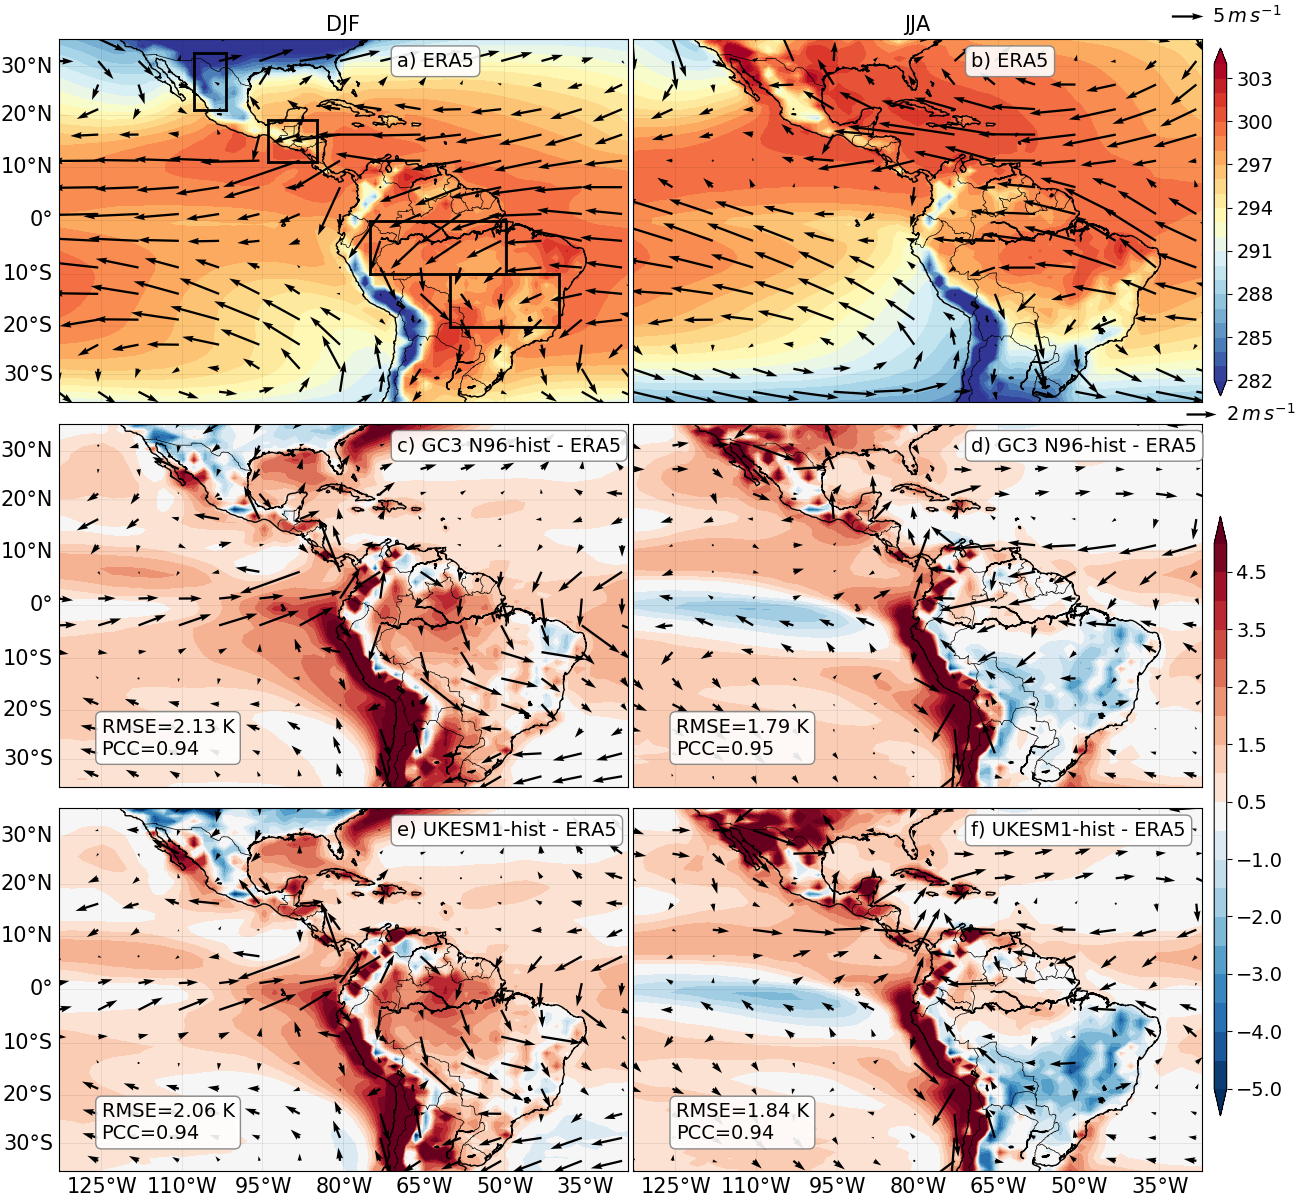
\includegraphics[width=\linewidth]{figures/fig1p2_f1a.png}
\caption[Temperature and SLP climatologies in UKESM1 and HadGEM3]{ (a, b) Temperature (color-contours in K) and wind speed (vectors) at 850 hPa DJF and JJA climatogies in ERA5. The biases are shown as the differences between the ensemble mean from the historical experiment of (c, d) GC3 N96 and  (e, f) UKESM1 and ERA5.
The climatogies and biases are shown for (a, c, e) boreal winter (DJF) and (b, d, f) boreal summer (JJA). Only differences statistically significant to the 95\% level are shown, according to a Welch t-test for each field. The key for the size of the wind vectors is shown in the top right corner of panels b) and d). The root-mean square error (RMSE) and pattern correlation coefficient (PCC) are shown on the bottom left of c-f.}
\label{fig:1}
\end{figure}

\begin{table}[t!]
\small
\caption{\small Root-mean square error (RMSE) and pattern correlation coefficients (PCC) for each season and each model experiment. Near surface air temperature ($t2m$), wind components ($u$ and $v$) and mean-sea level pressure ($mslp$) are assessed against ERA-5 and precipitation ($pr$) against TRMM.}
\begin{tabular}{p{1.05cm}|p{2.25cm}|p{1.10cm}p{1.10cm}p{1.10cm}p{1.10cm}p{1.10cm}p{0.9cm}p{1.05cm}p{1.05cm}} \label{tab:s1}
  \textit{Variable}                  & \textit{Experiment}  & DJF RMSE & DJF PCC & MAM RMSE & MAM PCC & JJA RMSE & JJA PCC &  SON RMSE & SON PCC \\ \hline \hline
t2m & GC3 N96 & 1.28 & 0.98 & 1.3 & 0.96 & 1.38 & 0.96 & 1.31 & 0.96 \\
t2m & GC3 N216 & 1.05 & 0.99 & 1.07 & 0.98 & 1.02 & 0.98 & 0.98 & 0.98 \\
t2m & GC3 Hist & 2.06 & 0.94 & 1.75 & 0.93 & 1.73 & 0.94 & 2.05 & 0.92 \\
t2m & UKESM-hist & 2.03 & 0.94 & 1.77 & 0.93 & 1.8 & 0.94 & 2.0 & 0.93 \\
t2m & GC3 AMIP & 1.17 & 0.98 & 1.12 & 0.97 & 1.2 & 0.97 & 1.2 & 0.97 \\
u & GC3 N96 & 0.78 & 0.99 & 0.59 & 0.99 & 0.9 & 0.98 & 0.87 & 0.98 \\
u & GC3 N216 & 0.78 & 0.99 & 0.59 & 0.99 & 0.9 & 0.98 & 0.87 & 0.98 \\
u & GC3 Hist & 1.02 & 0.98 & 1.04 & 0.97 & 0.92 & 0.98 & 0.84 & 0.98 \\
u & UKESM-hist & 1.04 & 0.98 & 1.01 & 0.97 & 0.91 & 0.98 & 0.82 & 0.98 \\
u & GC3 AMIP & 0.96 & 0.98 & 0.77 & 0.99 & 1.18 & 0.97 & 1.09 & 0.96 \\
v & GC3 N96 & 0.75 & 0.93 & 0.66 & 0.93 & 0.65 & 0.95 & 0.59 & 0.94 \\
v & GC3 N216 & 0.6 & 0.96 & 0.5 & 0.95 & 0.57 & 0.96 & 0.54 & 0.94 \\
v & GC3 Hist & 0.76 & 0.94 & 0.72 & 0.92 & 0.66 & 0.95 & 0.59 & 0.94 \\
v & UKESM-hist & 0.75 & 0.93 & 0.69 & 0.92 & 0.65 & 0.95 & 0.6 & 0.93 \\
v & GC3 AMIP & 0.67 & 0.95 & 0.52 & 0.95 & 0.68 & 0.94 & 0.61 & 0.93 \\
mslp & GC3 N96 & 1.33 & 0.96 & 1.03 & 0.97 & 1.15 & 0.96 & 0.95 & 0.97 \\
mslp & GC3 N216 & 1.11 & 0.97 & 0.9 & 0.97 & 1.1 & 0.96 & 0.89 & 0.97 \\
mslp & GC3 Hist & 1.31 & 0.97 & 1.12 & 0.96 & 1.08 & 0.96 & 0.94 & 0.97 \\
mslp & UKESM-hist & 1.4 & 0.97 & 1.15 & 0.96 & 1.14 & 0.95 & 0.99 & 0.97 \\
mslp & GC3 AMIP & 1.15 & 0.97 & 0.87 & 0.97 & 1.09 & 0.96 & 0.93 & 0.97 \\
pr & GC3 N96 & 2.02 & 0.79 & 2.24 & 0.71 & 1.62 & 0.9 & 1.69 & 0.86 \\
pr & GC3 N216 & 1.58 & 0.88 & 1.72 & 0.85 & 1.4 & 0.93 & 1.57 & 0.89 \\
pr & GC3 Hist & 2.05 & 0.78 & 2.49 & 0.64 & 1.69 & 0.88 & 1.69 & 0.86 \\
pr & UKESM-hist & 1.96 & 0.8 & 2.39 & 0.66 & 1.71 & 0.88 & 1.62 & 0.87 \\
pr & GC3 AMIP & 1.42 & 0.9 & 1.61 & 0.88 & 1.95 & 0.88 & 1.8 & 0.88 \\
\end{tabular}
\end{table}  

\begin{figure}[t!]
\centering
 %\noindent
 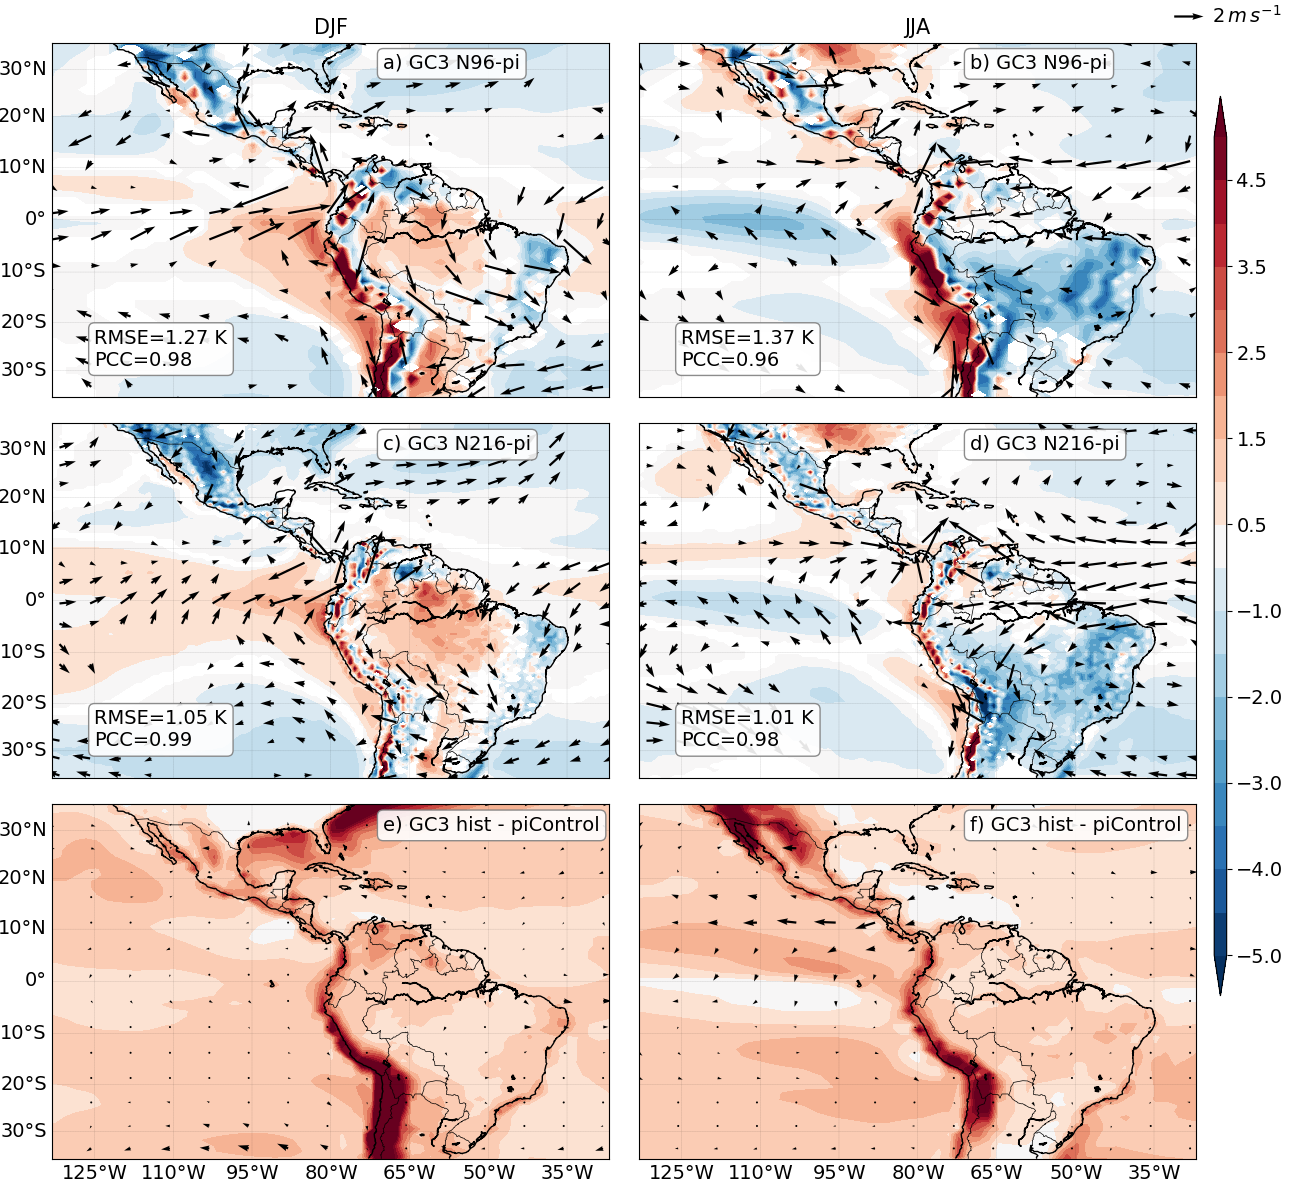
\includegraphics[width=\linewidth]{figures/fig1p2_f1b.png}
\caption[Temperature and SLP biases in UKESM1 and HadGEM3]{ As in Figure \ref{fig:1}, but showing the differences between the piControl simulations of (a, b) GC3 N96-pi and (c, d) GC3 N216-pi, and ERA5. (e, f) show the statistically significant differences between the historical (1979-2014) and piControl experiments of GC3.  The RMSE and PCC are shown on the bottom left of a-d.}
\label{fig:1b}
\end{figure}

 During DJF, the simulations show a colder-than-observed sub-tropical North America and a warm bias over the Amazon ($\approx +3.5$ K).
 The west coast of South America also shows a significant warm bias ($>+4$ K) in the historical simulations.
 The simulated circulation in austral summer in South America has a significant bias in the easterly flow coming from the equatorial and subtropical Atlantic.
 The low-level wind biases suggest a weaker easterly flow from the Atlantic into southeastern Brazil but also a strong southward flow from northern to southern South America.
  The South America Low-Level Jet, i.e., the low-level northwesterly flow in Bolivia, observed in Figure 1a, is stronger in the simulations.
   This stronger than observed jet is suggestive of a stronger moisture transport to the La Plata Basin, which has been associated with a drying of the Amazon and positive precipitation anomalies at the exit region of the jet \citep{marengo2012,jones2017}.
  % \citep


In turn, in boreal summer (Figures \ref{fig:1}d, f), positive temperature biases are observed in southwestern North America ($>+3.5 $ K), which are higher in UKESM1-hist than in GC3 N96-hist.
 The easterly flow west of Central America has a negative bias in UKESM1 suggesting a weaker flow that crosses from the Caribbean Sea into the East Pacific Ocean.
 %Both models show an anticyclonic anomaly in the region of the North Atlantic Subtropical High.
 Also in JJA, the simulated East Pacific surface temperatures are colder than observed for both historical experiments.      The inclusion of Earth System processes appears to make no  improvement on the low-level circulation biases. 

The piControl simulations (Figures \ref{fig:1b}a-d) have some similar biases to the historical simulations.
 In DJF, the piControl simulations show a similar positive bias in the Amazon than the historical experiments, although smaller, as well as a similar bias in the circulation in South America, with the smallest biases in GC3 N216-pi.
 In JJA, the piControl simulations do not show the positive temperature bias in northwestern North America observed in the historical experiments. However, the bias in the zonal wind over the easternmost Pacific is present in both piControl and historical simulations.
 
 Figures \ref{fig:1b}e, f show the difference between the historical and piControl experiment of GC3 N96, illustrating the response to historical forcing in GC3 N96.
 The temperature response in austral summer in South America is observed as 1.5 K whereas in JJA in North America temperatures were 4 K higher in the historical experiment than in the piControl.
 A very similar temperature pattern response to historical forcing was observed for UKESM1 (not shown) although of slightly different magnitude. The only significant difference in low-level winds, as a response to historical forcing, are the easterlies in the East Pacific Ocean during JJA, which are stronger in the historical simulation. %hereas the rest of the low-level wind

%The SLP and wind biases show that during boreal winter, a lower-than-observed SLP in southern South America of -2 hPa, is associated with a northwesterly wind anomaly into southeastern Brazil. This anomalous circulation is weaker in GC3.1 n216 than in the other two simulations.

\begin{figure}[t!]
\centering
 %\noindent
 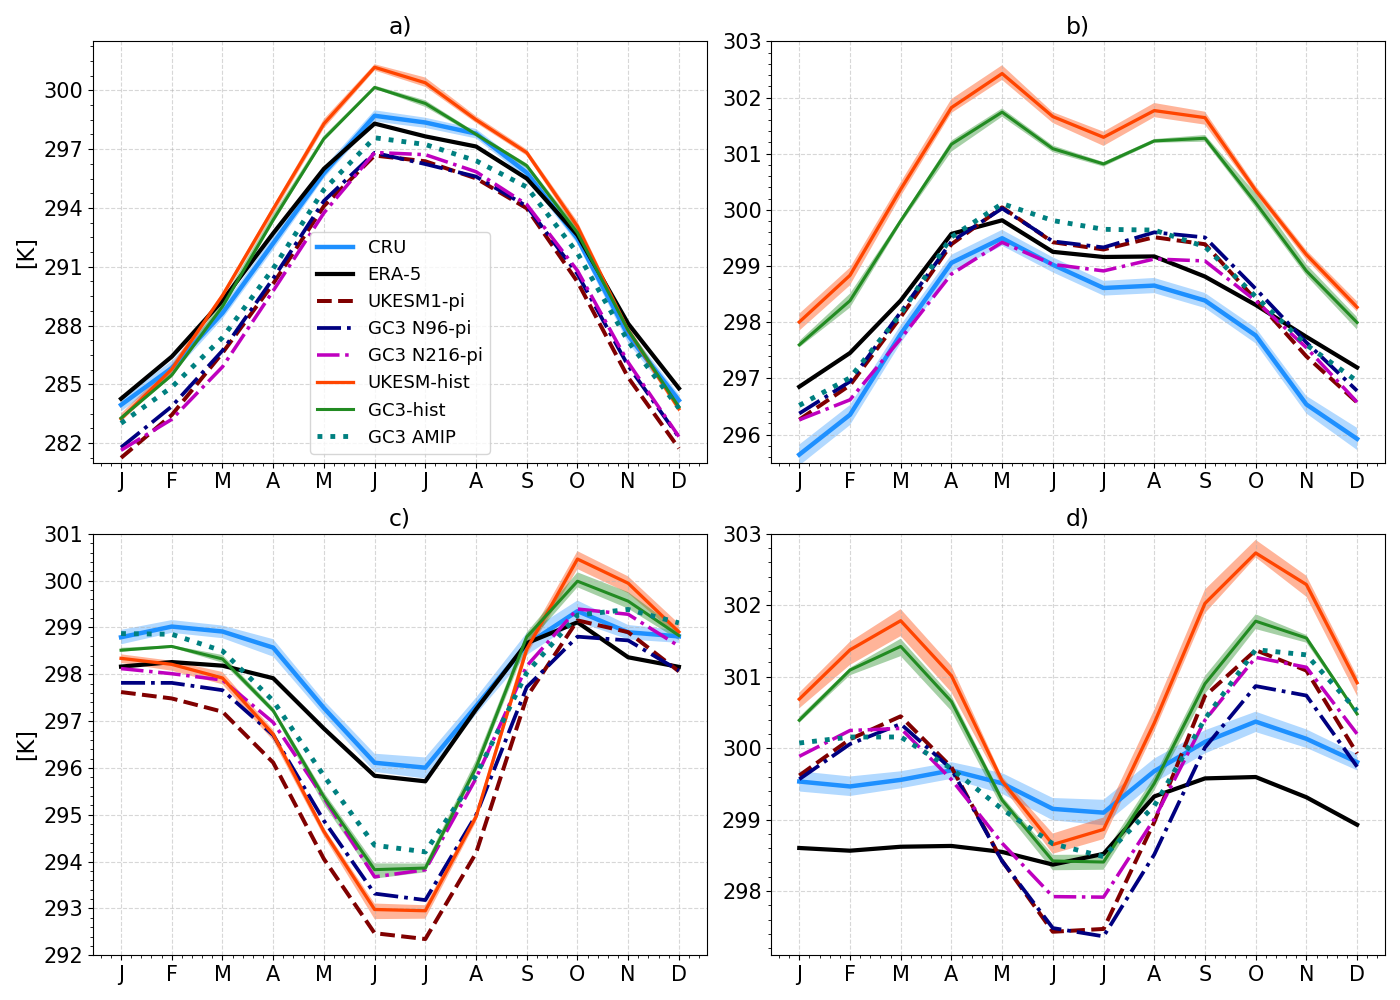
\includegraphics[width=\linewidth]{figures/p2fig2_v3.png}
\caption[Seasonal cycle of surface temperature in key monsoon regions]{ Monthly-mean temperature in the (a) North American Monsoon [19-35$^\circ$N,110-103$^\circ$W], (b) the Midsummer drought [11-19$^\circ$N,95-85$^\circ$W] (c) Eastern Brazil [20-10$^\circ$S,60-40$^\circ$W] and (d) the Amazon basin [-10-0$^\circ$S,75-50$^\circ$W] regions. The shadings for the CRU dataset represents the observational uncertainties and for the historical simulations the shading is the ensemble spread. The regions for this plot are shown in Figure \ref{fig:1}a. }
\label{fig:2}
\end{figure}

The seasonal cycle of temperature in key regions (depicted in Figure \ref{fig:1}a) of the AMS is shown in Figure \ref{fig:2}, comparing the simulations to ERA5 and the CRU4 dataset.
The temperature in the North American Monsoon region ranges from the boreal winter mean temperature of 12$^\circ$C to a maximum in June close to 27$^\circ$C.
Although the piControl simulated temperatures are colder than observed throughout the year, the models reasonably reproduce the seasonal cycle, which may be relevant for the simulated monsoon onset timing and strength \citep{turrent2009}. The historical experiments notably show a colder than observed winter and a warmer than observed summer.

The piControl simulations show a colder-than-observed winter in southern Mexico and northern Central America. The historical experiments show a warming signal, when compared to the piControl simulations, of about 1.5 K in winter and 2 K in the summer in this region. Despite these biases, all the experiments follow closely the seasonal cycle in North and Central America.

However, the seasonal cycle in South American regions (Figures \ref{fig:2} c, d) of southeastern Brazil and the central Amazon shows notable temperature biases.
The simulations show a stronger than observed seasonal cycle, especially the historical experiments. For example, the modelled temperature difference between late austral winter and spring was $\approx$4 K whereas the observed temperature varies by less than 1 K in the same period. The models show a warm bias in the Amazon region (Fig. \ref{fig:2} d) which peaks in austral spring (SON), during the development of the monsoon \citep{marengo2012}.
In southeastern Brazil, the seasonal cycle is reasonably well reproduced but with a significant cold bias throughout the year which maximizes during austral winter (JJA), as models (e.g. UKESM1) simulate  a temperature 4 K lower than observed.
In all panels of Figure \ref{fig:2}, the historical experiments show a significant warming signal as a response to historical forcing, which is generally stronger in UKESM1 than in GC3 N96. 


The near-surface air temperature and the low-level wind structure during monsoon season are intertwined with the processes that lead to monsoon rainfall which means that the biases presented in this section will likely be related to biases in precipitation, e.g., through cloud feedbacks. For example, a biased wind structure in eastern Brazil as well as the positive warm bias in the central Amazon during DJF may indicate biases in the moisture transport and cloud cover that lead to the dry Amazon bias \citep{jones2013}. The next section provides an assessment of a large-scale feature that is intimately related with monsoon rainfall:  the Intertropical Convergence Zones.

\section{The Atlantic and Pacific ITCZs and the SACZ}\label{sq:itcz}



The AMS is intertwined with the seasonal migration of the East Pacific and Atlantic ITCZ as the ITCZ largely determines regions of ascending and descending motions, moisture transport and the hemispheric energy balance \citep{oueslati2013,li2014,zhou2016,cai2019pantropical}. In particular, the North American monsoon and MSD are mostly influenced by the East Pacific ITCZ whereas the South American monsoon is affected by the strength and position of the Atlantic ITCZ \citep{yoon2010atlantic,marengo2012}. 
%This section validates the modelled ITCZs and Walker circulation.
%The ITCZ position is largely a result of atmospheric and oceanic energy transport \citep{schneider2014}, which are difficult to represent in GCMs and led to the double ITCZ problem \citep{li2014}.


Figure \ref{fig:3} shows the observed and modelled climatological rainfall and the ITCZ climatological positions. Three simulations are shown; two low-resolution (N96) runs, the ensemble-mean UKESM1-historical, the ensemble mean GC3 AMIP and a medium resolution run, GC3 N216-pi.
Other simulations are not shown as all the coupled low resolution (N96) simulations from UKESM1 and GC3 N96 showed very similar precipitation and ITCZ characteristics whereas the AMIP and medium-resolution experiments showed notable differences to the rest. 

\begin{figure}[t!]
\centering
 %\noindent
 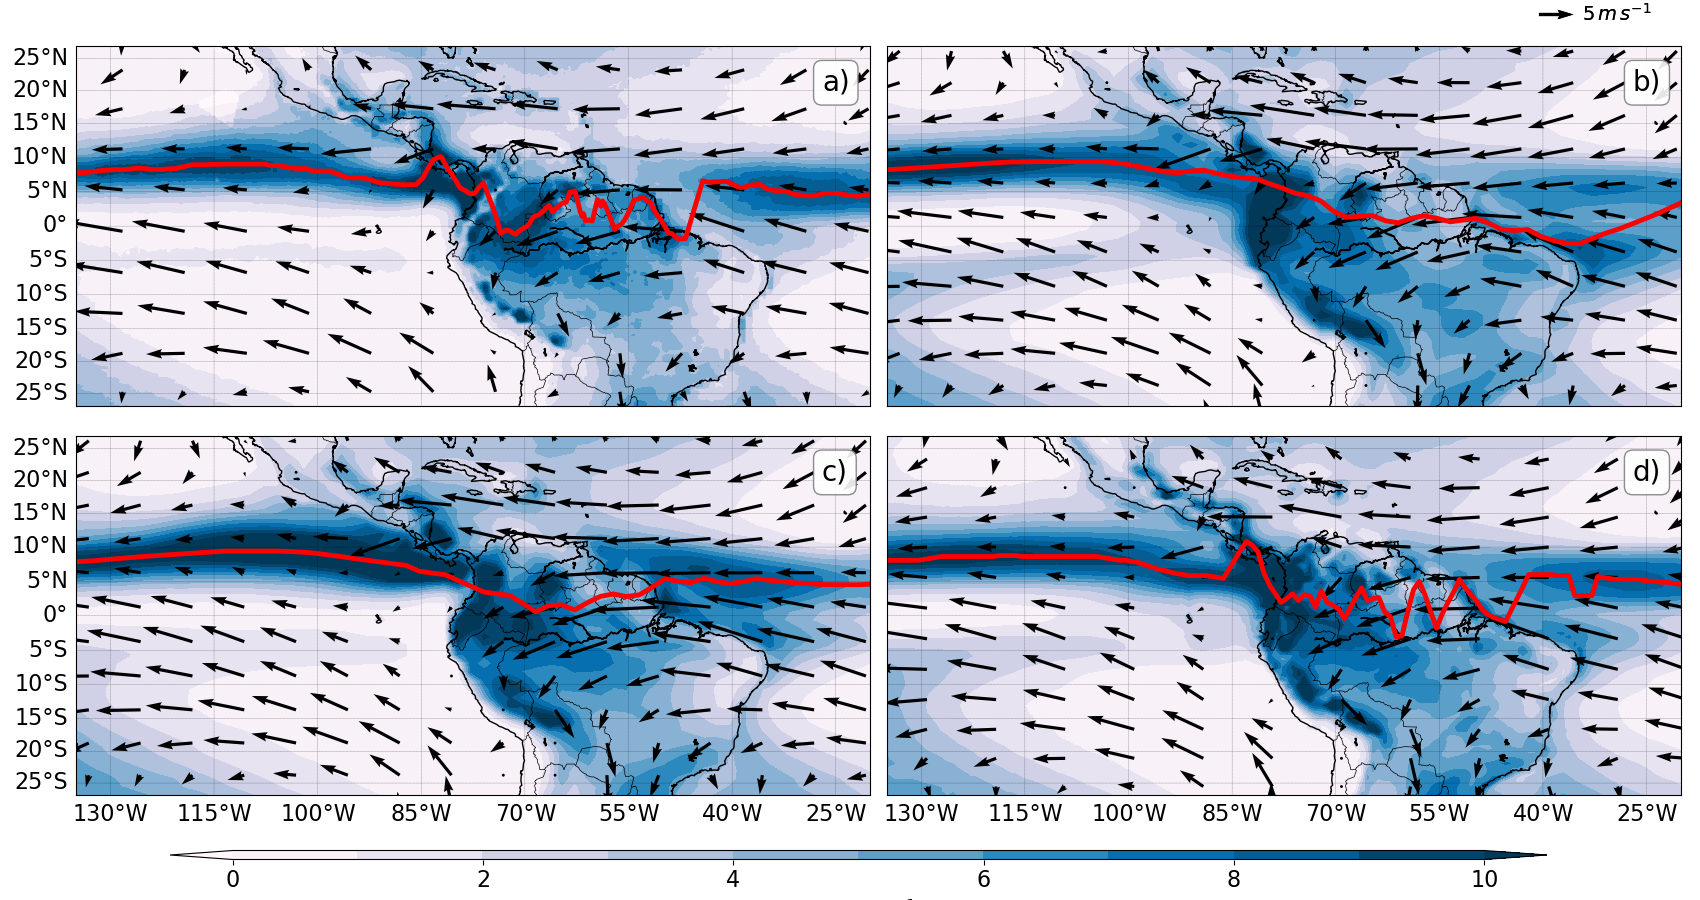
\includegraphics[width=\linewidth]{figures/itcz_clim_d.png}
\caption[Climatological precipitation and ITCZ position]{ Climatological precipitation [mm day$^{-1}$] and low-level wind speed (850-hPa) in (a) TRMM and ERA-5, (b) the ensemble-mean UKESM-historical, (c) GC3-amip and (d) GC3 N216-pi. The red line highlights the maximum rainfall for each longitude as a proxy for the position of the ITCZ.  }
\label{fig:3}
\end{figure}

The climatological ITCZ in TRMM (Figure \ref{fig:3}a) is found, on average, at 8$^\circ$N in the East Pacific and at 6$^\circ$N in the Atlantic.
All the simulations reasonably represent the climatological position of the East Pacific (EP) ITCZ; however, the modelled Atlantic ITCZ near the coast of Brazil is found south of the equator at 3$^\circ$S in the coupled model simulations.
The location of the ITCZ in GC3 N216-pi and the spatial distribution of rainfall is more consistent with TRMM dataset than the rest of experiments.
Rainfall near the Amazon river mouth is significantly larger in the low resolution simulations than in the TRMM dataset. 
 However, the GC3 AMIP shows the best agreement with TRMM in ITCZ position and rainfall distribution. 

\begin{figure}[t!]
\centering
 %\noindent
 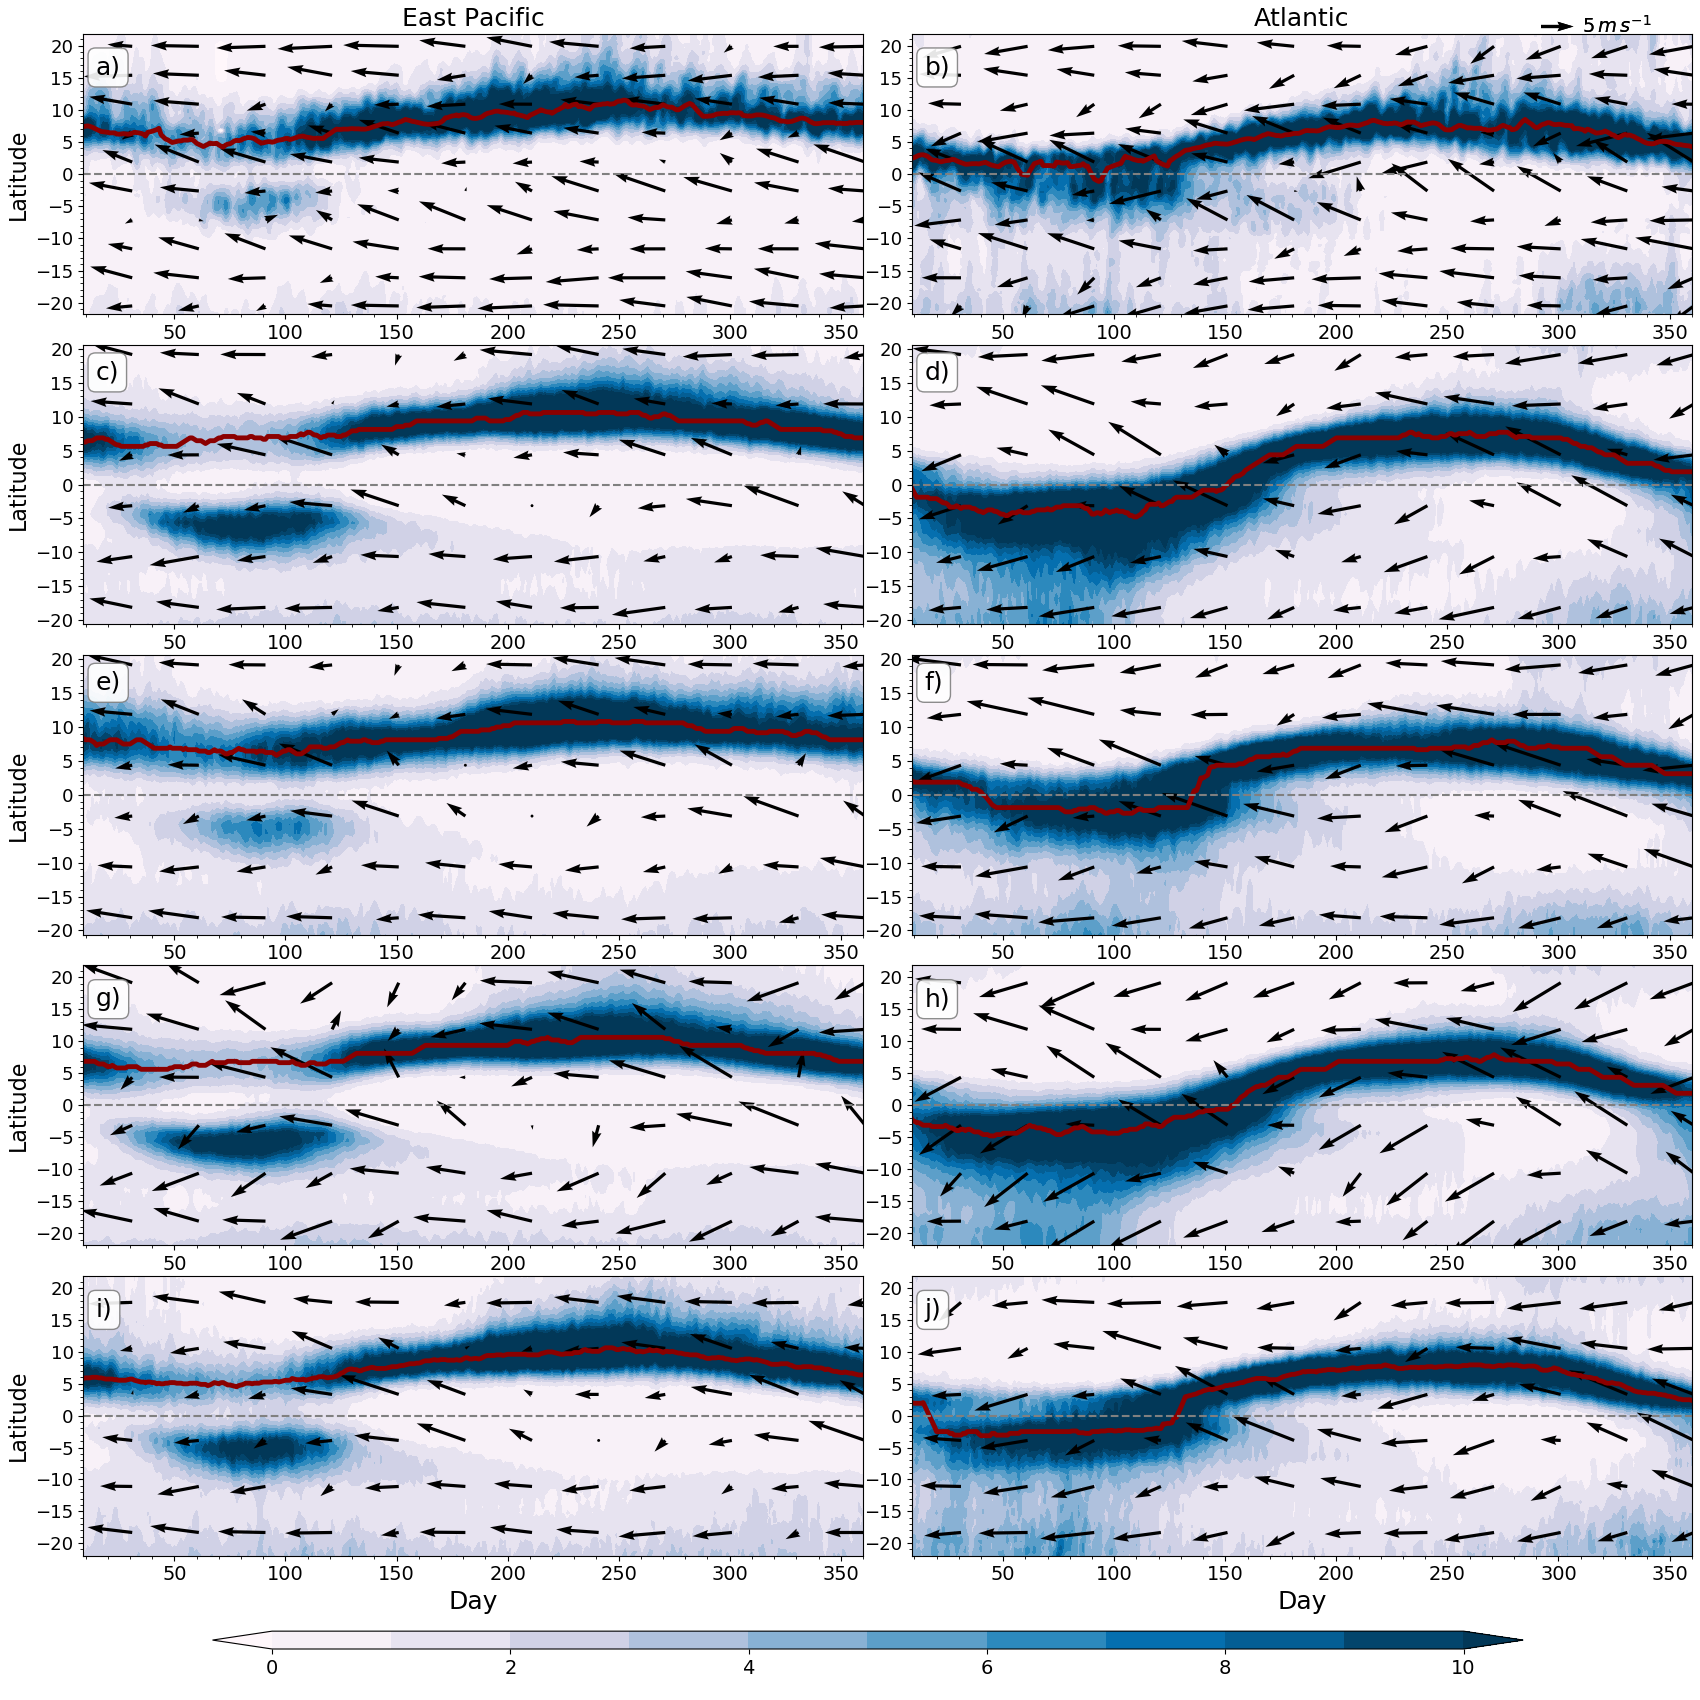
\includegraphics[width=\linewidth]{figures/fig3_p2_v3.png}
\caption[Seasonal evolution of Atlantic and Pacific ITCZ]{ Time-Latitude plot of daily mean rainfall (colour contours) and low-level wind speed (850 hPa) longitudinally averaged over the (a, c, e, g) East Pacific [150$^\circ$W-100$^\circ$W] and (b, d, f, h) Atlantic [40$^\circ$W-20$^\circ$W] Oceans. (a, b) show rainfall from TRMM and winds from ERA-5, (c, d) the ensemble-mean UKESM-historical, (e, f) GC3 AMIP, (g, h) GC3 N96-pi and (i, j) GC3 N216-pi. The red solid line shows the ITCZ as the latitude of maximum precipitation.  }
\label{fig:4}
\end{figure}


The seasonal cycle of the ITCZ location, precipitation rates and low-level winds in both basins are shown in Figure \ref{fig:4}, for TRMM, UKESM1-hist, GC3 AMIP, GC3 N96-pi and GC3 N216-pi.   %, two piControl and one historical simulations.
The EP ITCZ in observations (Fig. \ref{fig:4}a) migrates southwards during the first days of the year and is weakest and at its southernmost position at 5$^\circ$N around day 100 (mid-April).  
During boreal spring, the EP ITCZ migrates northward reaching a peak latitude and maximum rainfall at 10$^\circ$N by day 250, or early September. The EP ITCZ during boreal winter is weaker than during the rest of the seasons.
The low-level winds are predominantly easterly, which are stronger away from the ITCZ and weaker and convergent near the ITCZ position.
The position and seasonal migration of the EP ITCZ is reasonably well represented in the four simulations (Figs. \ref{fig:4}c, e, g, i), but a noticeable bias in precipitation is observed in  boreal winter south of the equator in the coupled simulations. The modelled  low-level winds in the coupled simulations show significant biases near the ITCZ.
These wind biases are observed as stronger wind vectors converging toward the ITCZ during boreal summer and spring and stronger wind vectors diverging away from the equator during boreal winter. 

The observed Atlantic ITCZ (Figure \ref{fig:4}b) has a similar seasonal cycle to the EP ITCZ.
The Atlantic ITCZ is close to 4$^\circ$N at day 1 and migrates southwards at the start of the year reaching  its southernmost position at 0$^\circ$ at the end of March.
During boreal spring, the Atlantic ITCZ migrates north, reaching 8$^\circ$N at the start of boreal summer. In contrast to the EP ITCZ, the maximum rainfall in the Atlantic ITCZ does not weaken during any season. 
The boreal winter position of the modelled ITCZ is displaced south with respect to the observations.
The simulated ITCZ  crosses south of the equator during boreal winter, with maximum precipitation rates of 12 mm day$^{-1}$ found in the 0-10$^\circ$S region.
After boreal spring, the modelled ITCZ crosses back north of the equator and matches the observed ITCZ reasonably well for boreal summer and fall.
Low-level wind vectors near the Atlantic ITCZ (Figures \ref{fig:4}f and h) suggest a simulated southerly bias north of the equator and a stronger northerly flow south of 10$^\circ$S.

The biases in the Atlantic ITCZ can also be observed in the Walker circulation as significant negative $\omega$ and $q$ biases just north and south of equatorial South America indicative of weaker convective activity. The Atlantic Ocean in the simulations shows a biased negative $\omega$ (more ascent) south of the equator and a positive $\omega$ bias (less ascent) north of the equator in the low resolution simulations.
The magnitude of the biases in the Atlantic ITCZ and overturning circulations described above were were associated with the horizontal resolution of the simulations. These biases were of similar magnitude in all the coupled model simulations run at the lower resolution N96, regardless of the type of experiment. However, these biases were reduced in the medium resolution experiments of GC3 N216 and in the GC3 N96 AMIP experiment which corrects SST biases (Figures \ref{fig:4}f, j). 

\begin{figure}[t!]
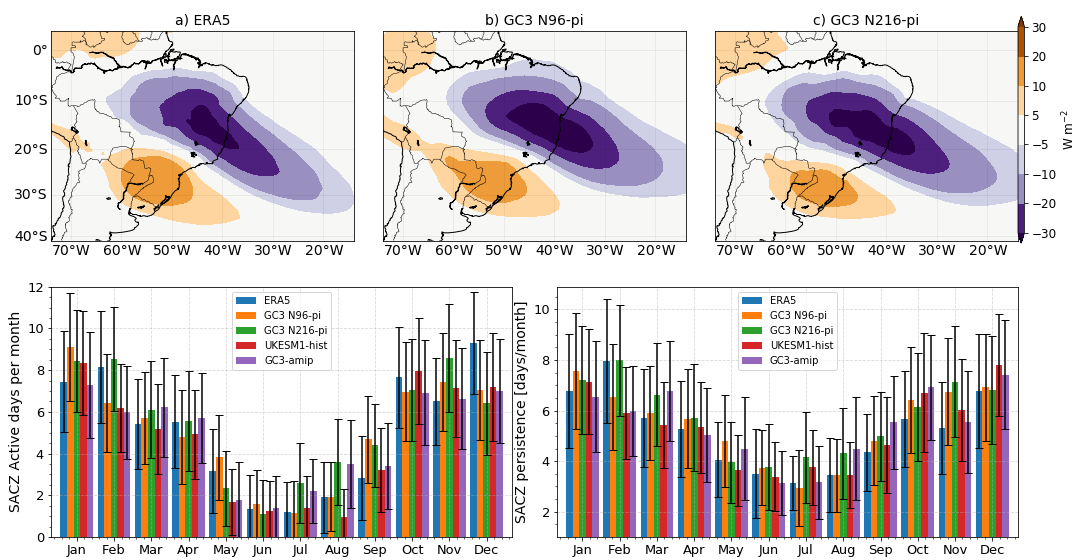
\includegraphics[width=\linewidth]{figures/saczanalysis.png}
\caption[SACZ assessment in UKESM1 and HadGEM3]{(a, b, c) OLR anomalies during active South Atlantic Convergence Zone (SACZ) events. (d, e) Frequency of active SACZ days and length of active SACZ events in reanalysis and model data, the standard deviation is shown as the error bar. The SACZ active days are constructed by first computing the first EOF of the monthly-mean deseasonalized OLR and then the daily OLR, previously filtered to remove periods higher than 99 days, is projected on the EOF pattern to produce a time series of pseudo-principal components. Active SACZ days are found when this time series of pseudo-PCs is greater than 1, and the persistence is measured as the number of continuous days where the time series is greater than 1.}
\label{fig:sacz}
\end{figure}

 The South Atlantic Convergence Zone (SACZ) is a nortwest-southeast oriented band of convection and is a prominent influence on the South American Monsoon mean and extreme rainfall \citep{carvalho2004,marengo2012,jorgetti2014}. The SACZ is primarily characterized by convergence oriented northwest-to-southeast that promotes rainfall in southeastern Brazil. The position of the SACZ and strength are an important factor for variability of the South American monsoon on different temporal and spatial scales \citep{carvalho2004,marengo2012,jorgetti2014}. 
 
 The SACZ in this simulations, defined by the outgoing long-wave radiation empirical orthogonal function analysis (Figure \ref{fig:sacz}) closely resembles the pattern found in ERA5. The SACZ active days and the persistence of the SACZ are also compared and found to be in relatively good agreement between reanalysis and model datasets.
The simulations from UKESM1, and GC3 N96 and N216 appear to reasonably simulate the spatial pattern of active SACZ days characterized by the low OLR in southeastern Brazil and higher OLR in the La Plata Basin. Similarly, the seasonal cycle of the frequency and persistence of SACZ active days is very well represented by the models with peak activity found from November through January and very little activity during austral winter. The impact that an accurate representation of the SACZ activity in GCMs has for representing short-scale variability of the South American Monsoon System is an open question, as the SACZ is rarely assessed in CMIP analyses.

GCMs have showed little improvement in their representation of ITCZs \citep{oueslati2015}. This bias has persisted through CMIP phases largely because the position, strength and seasonal migration of the ITCZ is hard to represent accurately. These features are controlled by ocean-atmosphere feedbacks that intertwine the local and regional circulation with cloud-radiative feedbacks and the atmospheric and oceanic transport of energy \citep{schneider2014,oueslati2015,byrne2016,byrne2020}. 
This section shows that the CMIP6 MOHC models reasonably simulate the location of the East Pacific ITCZ but poorly represent the location of the austral summer Atlantic ITCZ and overestimate precipitation over the East Pacific ITCZ. The location and seasonal variability of the SACZ is also fairly well simulated by all the models. The implication of the results in this section for AMS precipitation will be addressed in the last section this chapter.


\section{Precipitation and convection in the AMS}\label{sq:precip}
%This section compares the spatial and temporal distribution of rainfall in four key regions of the AMS between observations and reanalysis, and the simulations, as well as other characteristics of convective activity, such as height and strength. %, are compared to better understand convective representation in this region.

\subsection{Mean seasonal precipitation}

\begin{figure}[t!]
\centering
 %\noindent
 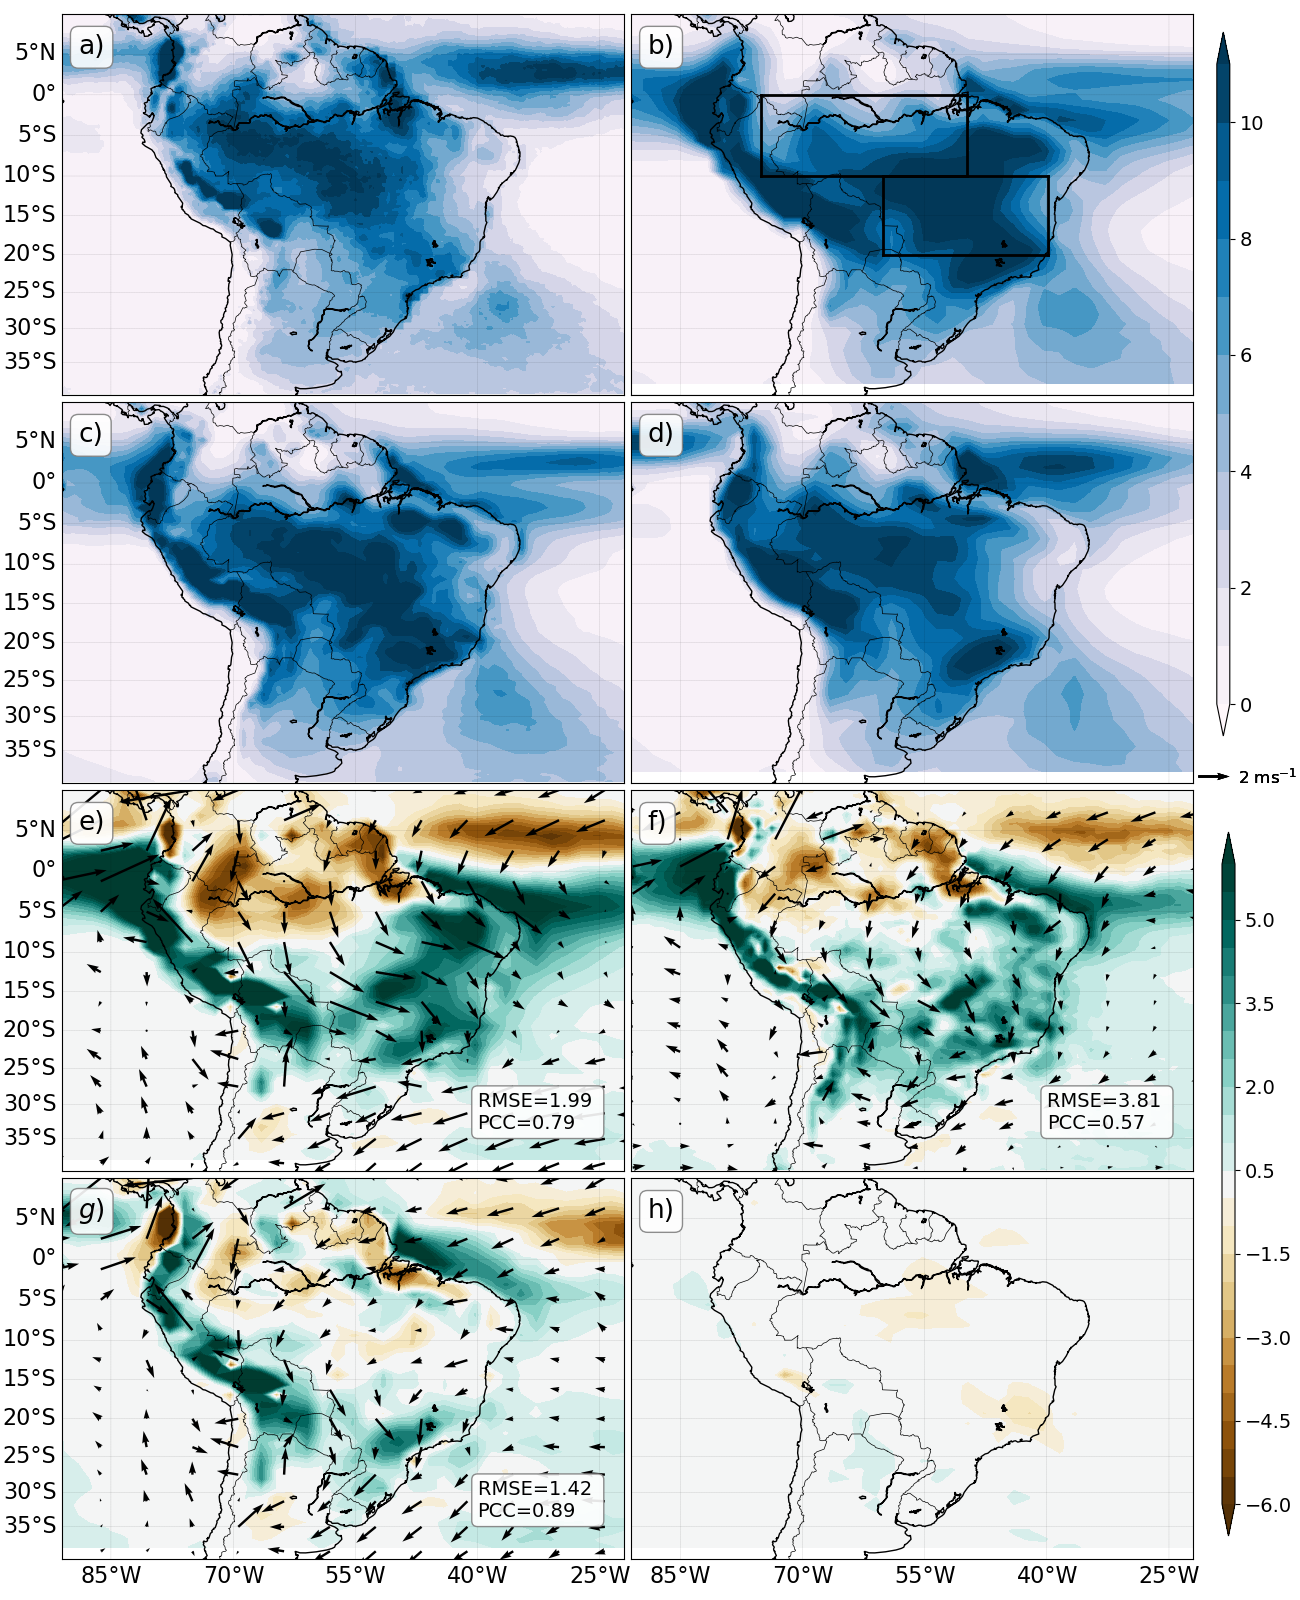
\includegraphics[width=0.875\linewidth]{figures/fig6.png}
\caption[Austral summer mean rainfall in the South American monsoon]{ DJF mean rainfall [mm day$^{-1}$] from (a) TRMM, (b) UKESM1-historical, (c) GC3 N216-pi and (d) GC3-amip. (e, f, g) show the statistically significant differences between panels (b, c ,d) and (a) TRMM, respectively. (h) Precipitation difference between UKESM-historical and  UKESM1-pi, only statistically significant differences (95\%) confidence level is shown.  The biases in the 850-hPa winds are shown as vectors. }
\label{fig:6}
\end{figure}

  The austral summer (DJF) rainfall distribution in South America of the TRMM dataset and the simulations for GC3 N216-pi, UKESM-hist and GC3-amip (Figure \ref{fig:6}) shows several noteworthy biases in the coupled simulations. 
The maximum austral summer rainfall in TRMM
(Figure \ref{fig:6}a) is found as a northwest-southeast oriented band of precipitation from the core Amazon region into southeastern Brazil, which is related to the SACZ.
The biases are illustrated (Figures \ref{fig:6}e-h) as the precipitation difference between the simulations and TRMM.
 
%The coupled simulations (e.g. Figure \ref{fig:6}b, c) overestimate rainfall in southeastern Brazil and underestimate rainfall in the core Amazon region.
 

   The coupled simulations show three main biases.
Rainfall in the Atlantic ITCZ in these simulations is displaced southwards, observed as positive (+5 mm day$^{-1}$) biases south of the equator and negative biases ($-$5 mm day$^{-1}$) north of the equator in the Atlantic.
Second, the models underestimate rainfall in the core Amazon basin by $-$3 mm day$^{-1}$ on average, and the third major bias is that rainfall in southeastern Brazil is overestimated by more than +5 mm day$^{-1}$, approximately +100\% of the observed rainfall in this region.  

 The precipitation biases are associated with a stronger northerly flow in South America, transporting moisture from the Amazon into southeastern Brazil and the La Plata Basin.   
The magnitude of these biases is smaller in GC3 N216 (Figure \ref{fig:6}f) than in the low resolution simulations, such as UKESM1-hist.   The ensemble mean GC3 AMIP (Figure \ref{fig:6}d) shows a better representation of the austral summer rainfall and circulation patterns, removing the main circulation biases (Figure \ref{fig:6}g) of the coupled simulations.   
The response to historical forcing, illustrated by the difference between UKESM1-hist and UKESM1-pi (Figure \ref{fig:6}h), is much weaker than the magnitude of the biases and is characterized by a weak drying of the Amazon and southeastern Brazil. Therefore, the magnitude of these biases are too large to have confidence in these drying responses to historical forcing. 


\begin{figure}
\centering
 %\noindent
 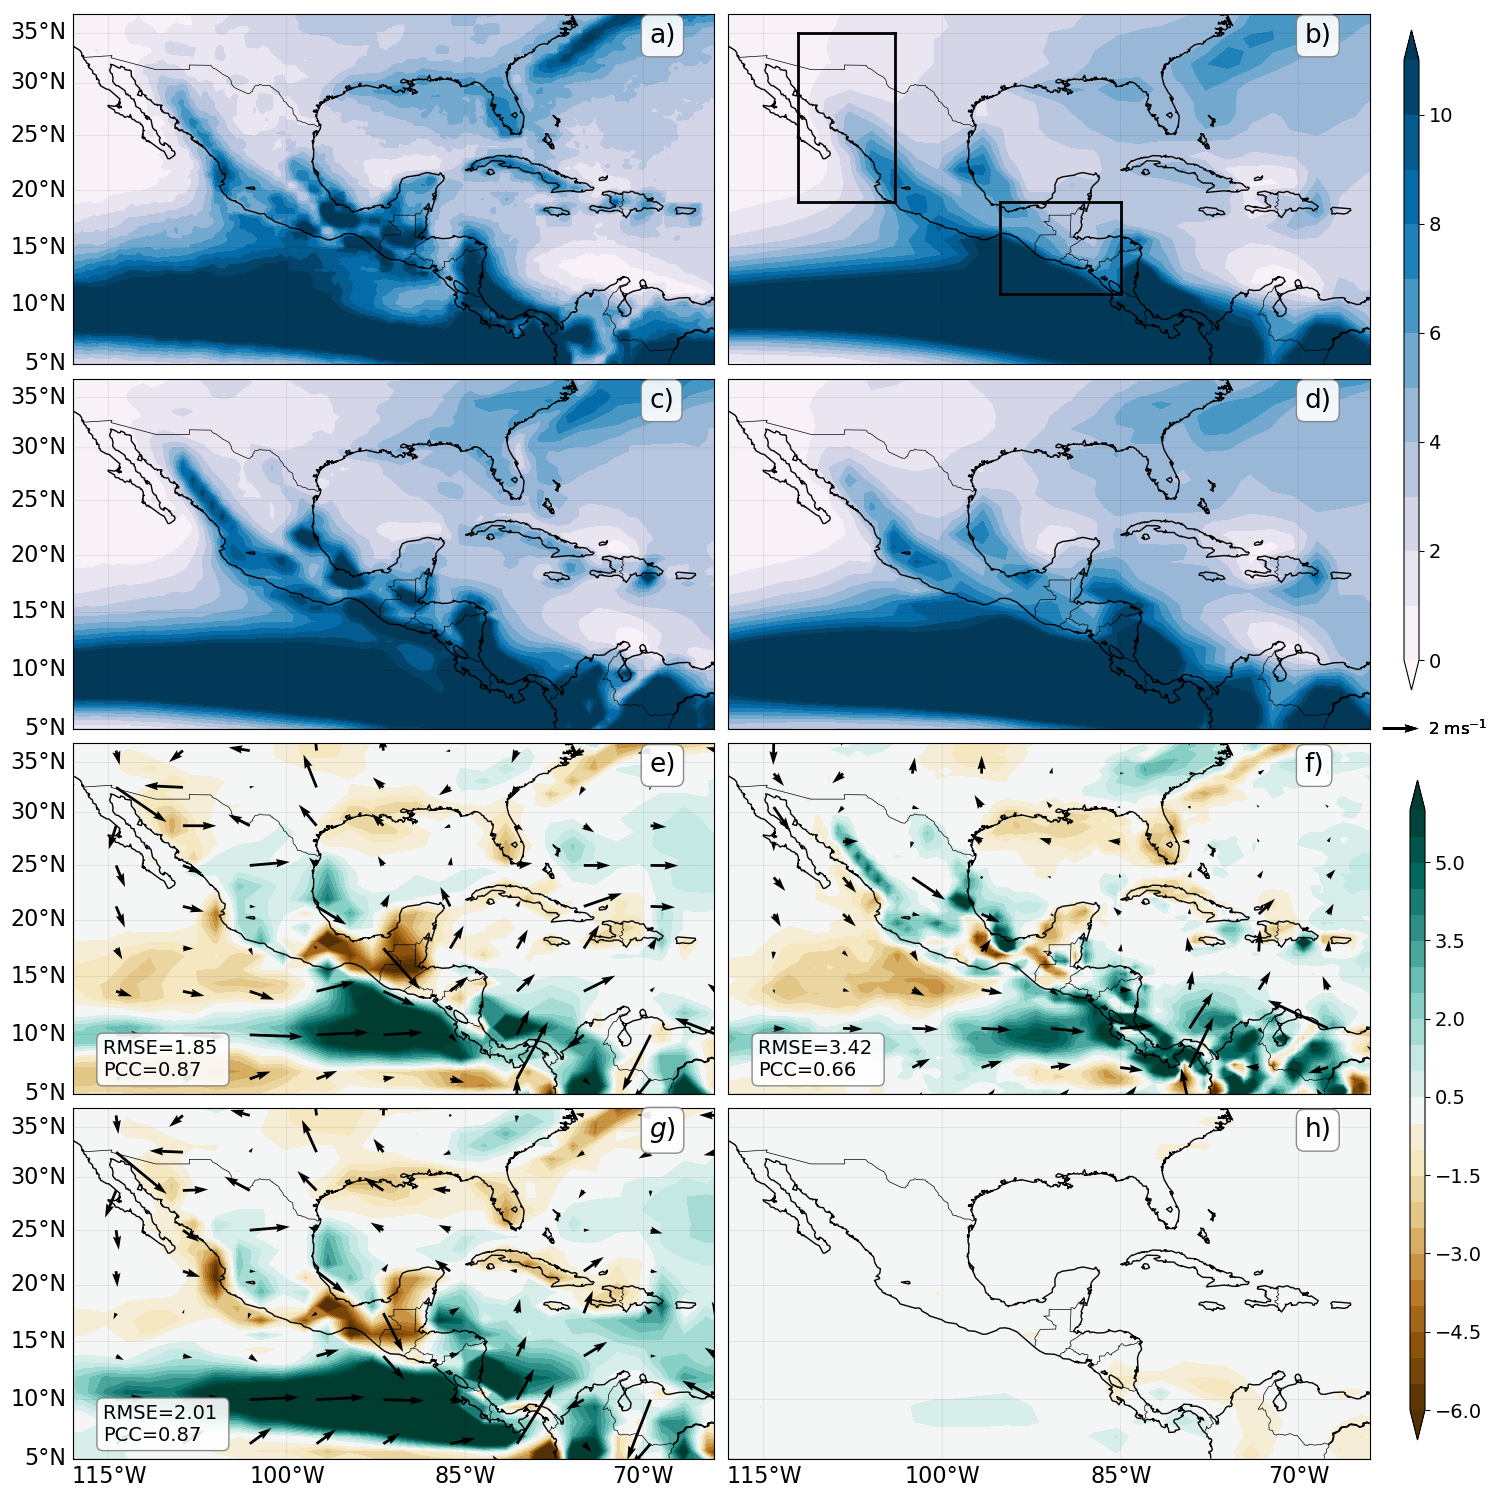
\includegraphics[width=\linewidth]{figures/Fig8.png}
\caption[Boreal summer precipitation in the North American Monsoon]{ As in Figure \ref{fig:6} but for JJA in the northern part of subtropical America.   }
\label{fig:7}
\end{figure}

The modelled and observed JJA mean rainfall and biases for Mexico and Central America are shown in Figure \ref{fig:7}.
The main feature is the East Pacific (EP) ITCZ which extends north to 15$^\circ$N near the western coast of Mexico as a broad band of rainfall (>11 mm day$^{-1}$).
 The modelled EP ITCZ (Figures \ref{fig:7}e, f, g) rainfall is overestimated by more than 5 mm day$^{-1}$, especially in GC3-amip. This wet bias is associated with a westerly bias in the low-level circulation, suggesting a weaker flow from the Caribbean into the East Pacific.

The North American Monsoon can be observed as a band of precipitation across western Mexico. In the core monsoon region, near the Sierra Madre Occidental \citep{adams1997, zhou2016}, the JJA-mean rainfall is higher than 8 mm day$^{-1}$. %Several regions in southern Mexico also exhibit large seasonal mean rainfalls.
The distribution of rainfall in the North American Monsoon region is relatively well represented in all the simulations, as only a moderate wet bias (+2 mm day$^{-1}$) in western Mexico is observed.
The northernmost part of the North American Monsoon (southwestern US) is best simulated by GC3 N216-pi, as the other simulations show a dry bias in this region.
%This positive bias extends to southern Central America.
The low-resolution simulations (Figure \ref{fig:7}e) underestimate rainfall (-5 mm day$^{-1}$) over land in southern Mexico, Guatemala and Belize.
Rainfall in the Caribbean islands and Florida is underestimated (-1 mm day$^{-1}$) in all simulations.

In most cases for JJA in this region, the precipitation and wind biases were reduced in the high-resolution simulation (Figure \ref{fig:7}f) and little-to-no difference was observed between UKESM1-hist and GC3 N96-hist (not shown).
The precipitation response to historical forcing is much lower than the biases (Figure \ref{fig:7}h) with no significant precipitation differences over land due to the historical forcing. % shows a decrease in precipitation.
 

\subsection{The annual cycle of rainfall}\label{sq:raincycle}

\begin{figure}[b!]
\centering
 %\noindent
 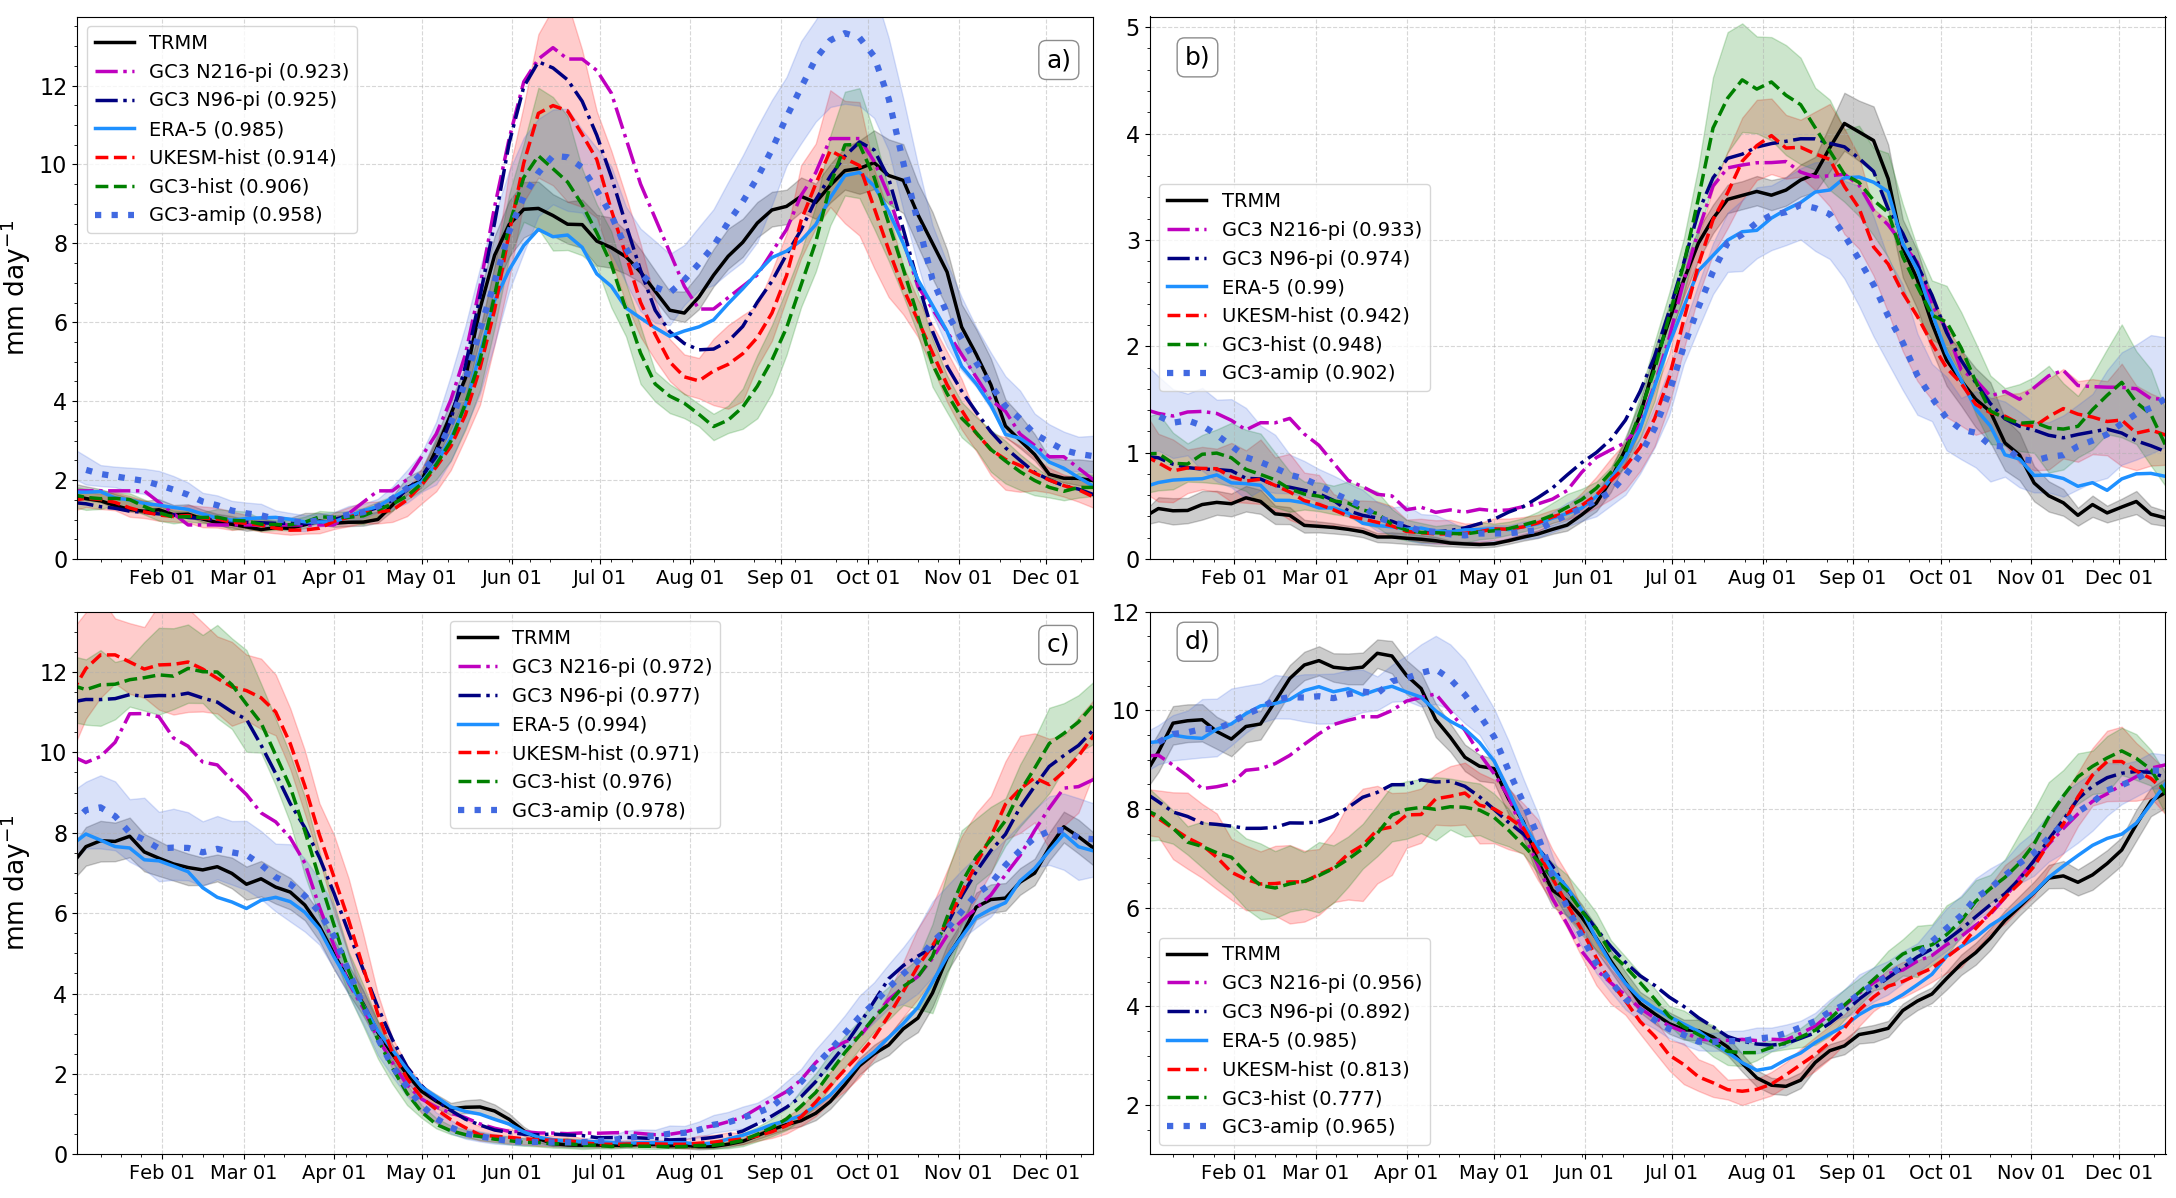
\includegraphics[width=1.0\linewidth]{figures/amipseasonalcycle.png}
\caption[Annual cycle of precipitation in different regions of the AMS]{Annual cycle of pentad-mean rainfall in the regions (a) the Midsummer drought, (b) the North American Monsoon, (c) Eastern Brazil and (d) the Amazon Basin. The regions are defined as in Figure \ref{fig:2} and are illustrated in Figure \ref{fig:7}b and Figure \ref{fig:8}b. The shaded regions represent observational uncertainty for TRMM and ensemble spread for the historical experiments. The correlation coefficient for each of the simulated seasonal cycles with TRMM is given in brackets in each panel.  }
\label{fig:8}
\end{figure}

%CMIP assessments typically evaluate rainfall model performance by inspecting area-averaged monthly-mean evolution of rainfall.
%However, this temporal resolution is not enough to properly evaluate the performance of a simulation, particularly in monsoonal regions where the dates of monsoon onset and demise have relevance for sectors such as agriculture.

Figure \ref{fig:8} shows the seasonal cycle of rainfall at the pentad (5-day) scale over the North American Monsoon, the  Midsummer drought (MSD), the Amazon and eastern Brazil regions. The correlation between TRMM and the model and reanalysis data (ERA5) is also shown in each panel. 
The seasonal cycle of precipitation in the MSD region in the simulations is well represented as all the simulations show the characteristic bimodal distribution, a feature that is uncommon for a climate model to be able to reproduce \citep{ryu2014}.
%This peculiar bimodal distribution of rainfall is characterised by a first rainfall maxima in June and a second maximum in late September, separated by a relatively drier period with a minimum at the start of August. The Midsummer drought bimodal distribution was only found in a handful of CMIP5 models \citep{yin2013}.
However, the characteristics of the simulated MSD are different from observations.
For example, the magnitude of the first peak and second peaks in the simulations are different. 
For instance, most of the first peak simulated magnitudes are higher than TRMM by 4 mm day$^{-1}$, and the AMIP simulation overestimates the second maximum of rainfall by 2-3 mm day$^{-1}$. Similarly, the differences between the first peak and the MSD and between the MSD and the second peak are more pronounced in the coupled simulations. The timing of the MSD period is different in the models, as the simulations show the driest period taking place 10 days after TRMM and ERA5. %  All the simulations show different magnitudes of the first and second peak and the MSD precipitation, 
 
 

In the North American Monsoon (Figure \ref{fig:8}b), the observed seasonal cycle is characterized by a very long and dry period ranging from the end of November to the start of June, which is followed by a sharp increase of rainfall around mid-June. The timing of the increase of rainfall in models coincides with observations, suggesting that onset timing and strength is well represented in these models.
Moreover, the modelled and observed mean precipitation rates during monsoon maturity are $~$4 mm day$^{-1}$, from mid-July until early September, which suggests notable ability of the models to reproduce the peak monsoon rainfall.
%The timing of monsoon retreat is also well represented by the simulations, as both modelled and observed rainfall decay during September.
   The historical simulations show a shorter wet season characterised by an earlier retreat of the monsoon rainfall and, as in all the simulations a positive bias (+1 mm day$^{-1}$) is found during late local fall and early winter, a feature that has been shown in these models in CMIP5 \citep{geil2013}. % and that will be further explored in the following chapter. %For instance, GC3 N96-hist retreats on average around August 16th. 
%However, winter-time rainfall, before monsoon onset and after monsoon retreat, is overestimated by all the simulations, particularly the higher resolution GC3.1 N216 which has a positive bias of $~$2 mm day$^{-1}$ in early winter. 


The seasonal cycle of precipitation in eastern Brazil is characterised by a very wet summer ($\sim$8 mm day$^{-1}$) compared to a very dry ($\sim$0.2 mm day$^{-1}$) winter (Figure \ref{fig:8}c).
%The South Atlantic Convergence Zone has a centre of action over this region and thus controls several aspects of precipitation \citep{carvalho2004,marengo2012}.
Rainfall in TRMM and ERA5 increases steadily from austral spring (September) to a maximum found in early January ($\sim$8 mm day$^{-1}$).
Rainfall in this region decreases to $\sim$6 mm day$^{-1}$ by late March as the monsoon migrates northward and then sharply decreases in austral fall.


The models (Figure \ref{fig:8}c) show a positive bias during monsoon maturity. This bias was found to be of +4 mm day$^{-1}$ and +2.5 mm day$^{-1}$ for the low and medium resolution simulations, respectively.
This positive bias in the maximum rainfall is consistent with the biases shown in Figure \ref{fig:6}, which showed that rainfall in southeastern Brazil is overestimated, especially in the low resolution coupled simulations.   In contrast to the coupled simulations, GC3-amip shows a very good agreement with the observed maximum summer rainfall and the seasonal cycle (r=0.978) throughout the year.
%Despite this positive bias in the magnitude of precipitation, the seasonal evolution of rainfall is very well represented by the simulations, as the onset and retreat dates are in close agreement with the observations.

Finally, the seasonal cycle in the Amazon (Figure \ref{fig:8}d) has a weaker contrast as rainfall greater than 2 mm day$^{-1}$ is found year-round. The coupled simulations show a dry bias during austral summer and a good agreement with the observations during austral winter. Rainfall rates in the Amazon from January to March, in both TRMM and ERA-5, is close to 10 mm day$^{-1}$, yet the low resolution simulations show rainfall rates of 8 mm day$^{-1}$ in mid-February, particularly the historical experiments.
GC3 N216-pi shows a better agreement with observations but still underestimates summertime rainfall by 1 mm day$^{-1}$.   

This dry Amazon bias has been a known feature of GCMs, including the MOHC models, since CMIP3 \citep{li2006,yin2013}. In these simulations the dry Amazon bias is only alleviated in GC3-amip whose seasonal cycle and maximum summer rainfall agree well with observations suggesting that the Atlantic SST biases are the key factor for the biases in the Amazon in coupled model simulations.   
% Peak summertime rainfall is underestimated by the coupled model simulations, particularly the historical experiments. 
The models, however, represent with reasonable skill the timing of the transition from
early austral spring (4 mm day$^{-1}$ in September) to summertime rainfall (6 mm day$^{-1}$ in November).
%The low resolution simulations, after simulating an annual maximum of rainfall in December, simulate a decrease in precipitation for January and February, whereas the observations show the opposite behaviour.
After this description of the spatial and temporal variability of these biases in these models, the next section investigates how the models represent convection through diagnostics that may further 

\subsection{Characteristics of convective activity}

The seasonal cycles of outgoing long-wave radiation (OLR), vertical velocity ($\omega$) and specific humidity ($q$) are key features of a monsoon since these quantities characterise the strength and height of deep convection, as well as the moisture within the column.
 The pentad-mean annual cycle of OLR, $q$ and $\omega$ at the 500-hPa level in four regions of the AMS (Figure \ref{fig:9}) are used as process oriented diagnostics to further evaluate the biases in the spatial distribution and seasonal cycle of rainfall.
 

For the North American Monsoon the seasonal cycle of OLR, $q$ and $\omega$ is relatively well represented in the simulations.
During late boreal winter and early spring, OLR increases steadily as a result of surface warming.
However, in early June, near the onset date \citep{douglas1993,geil2013}, OLR sharply decreases reaching a minimum value of 246 W m$^{-2}$ by mid-July.
The vertical velocity decreases steadily from January to a minimum in August, indicating ascent from May 1st until September 15th.
 The models show similar seasonal cycles but overestimate the summertime OLR by $\approx$ 6 W m$^{-2}$ and underestimate mid-level moisture by 0.3 g/kg and $\omega$ by 0.01 Pa s$^{-1}$ which is about 5-10\% overall. 
%After convective activity decreases in late August in ERA-5, OLR increases to a local maxima of $\sim$ 271 W m$^{-2}$ on mid-September, $q$ decreases significantly and $\omega$ turns positive.
The simulated shallower convection and drier mid-troposphere is seemingly compensated by stronger mid-level ascent.


\begin{figure}[t!]
\centering
 %\noindent
 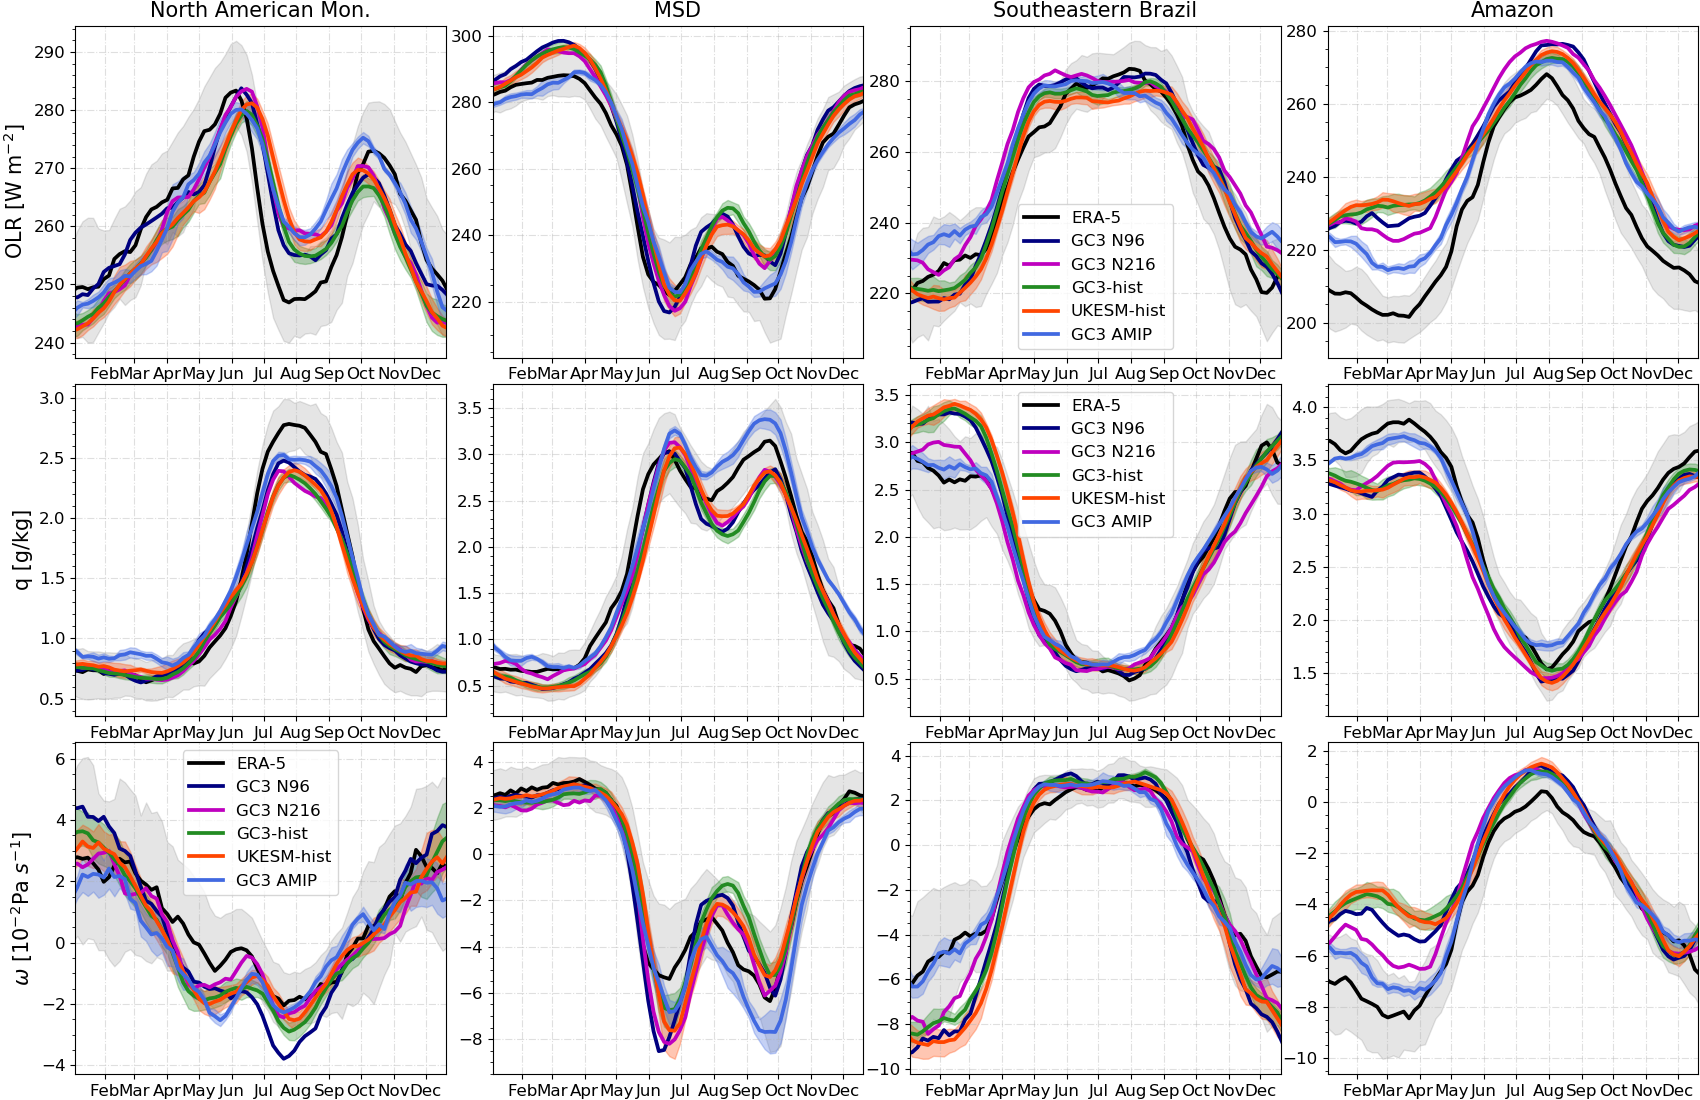
\includegraphics[width=\linewidth]{figures/fig9b.png}
\caption[Seasonal cycle of measures of convection in the AMS]{Pentad-mean (upper) outgoing long-wave radiation (OLR), (middle) specific humidity at 500-hPa and (lower) $\omega$ 500-hPa. These are shown from left to right for the North American Monsoon, the Midsummer drought, southeastern Brazil and the core Amazon. The uncertainty in ERA-5 data, shown as faint gray shading was estimating by bootstrapping with replacement the ERA-5 record 10,000 times. }
\label{fig:9}
\end{figure}

In the MSD region, OLR and $q$ show signs of convective activity from mid-April, as OLR sharply decreases and moisture increases.
%The key characteristic of the MSD is the modest decrease in rainfall in the midsummer.
The characteristic MSD bimodal distribution of precipitation can also be observed as two troughs of OLR, and $\omega$ and two peaks in $q$.
These periods are separated by a period of relatively higher OLR, lower $q$ and weaker ascent from June 15 until late August.
%The reanalysis data shows that during the MSD period OLR increases by 10 W m$^{-2}$, $\omega$ decreases by 0.015 Pa s$^{-1}$ and $q$ decreases by 0.5 g/kg.
Although arguably with a small dry bias with shallower convection after mid-July, the simulations follow closely the observed seasonal cycle.

The simulated conditions during the first peak period show similar OLR and mid-level moisture but stronger ascending motions, which may explain the positive rainfall bias in this period showed in Figure \ref{fig:8}a.
In the period between the first peak and the MSD, the simulated OLR increases more sharply than observations from 220 W m$^{-2}$ (June 15) to 250 W m$^{-2}$ (early August), with similar behaviour in $\omega$ and $q$, which may also be related to the strong MSD precipitation differences described in the previous section.
%In the same period, the simulated moisture and ascent decrease more sharply than observations, in agreement with the stronger variations of precipitation (Figure \ref{fig:8}a).
%The stronger than observed changes to the characteristics of convection are consistent with the sharper than observed midsummer drought in the simulations showed in Figure \ref{fig:8}a.
The period during the second peak of rainfall in September shows signs of shallower convection and a drier mid-level when compared to ERA5.
%The characteristics of the retreat stage of rainfall at the start of October shows close agreement between reanalysis and simulations.
%Overall, the models seem to reproduce the annual cycle of OLR and

In southeastern Brazil, the simulations reasonably follow the timings of the annual cycle of OLR, $q$ and $\omega$ of the reanalysis, particularly during austral winter. The moisture $q$ in ERA5 during  the dry seasons of austral fall, winter and spring is reasonably simulated by all the experiments. However, during austral summer, the coupled model simulations show significant biases characterised by stronger ascent and increased specific humidity in the mid-levels, although the height of convection (OLR~ 225 W m$^{-2}$) is only modestly higher in the simulations.

%The seasonal cycle of these proxies for convective activity in the Amazon basin are shown by Figure \ref{fig:8}.
The simulated OLR, q and $\omega$ exhibit the highest biases in the Amazon. During austral summer, particularly January and February, the simulated convective activity is shallower (OLR bias of +25 W m$^{-2}$) and weaker (positive $\omega$ bias +0.02 Pa s$^{-1}$) and the mid-level troposphere is drier (~-0.5 g/kg) than in ERA5. All these biases are in agreement with the dry Amazon bias described in the previous section. Despite biases in the magnitude of OLR, $q$ and $\omega$ during peak convective activity, the seasonal variation is very well simulated so that convective activity, as evidenced by these metrics, starts and ends in the simulations within one or two pentads of the reanalysis. The smallest biases in coupled simulations are those of GC3 N216-pi, not just for the Amazon region but for the other regions as well.  The simulated OLR, $q$ and $\omega$ in GC3-amip in southeastern Brazil and the Amazon show a much better agreement with the reanalysis during austral summer than the rest of the simulations.

This section describes biases in the seasonal cycle of diagnostics intimately related to convection such as top cloud height, vertical velocity and moisture. While precipitation is fairly well represented in the North American monsoon in this region, the models represent stronger but shallower ascent indicating that competing biases lead to a right representation of precipitation. 


\section{ENSO Teleconnections}\label{sq:enso1}

El Ni\~no-Southern Oscillation (ENSO) teleconnections are the prominent source of interannual variability for the AMS \citep{vera2006}, as summarized in section \ref{sub:lit_enso}.
The response to ENSO events in UKESM1 and HadGEM3 is investigated in this section, which first shows the temperature, sea-level pressure (SLP) and precipitation responses  to observed and simulated ENSO events in the AMS, and then analyses of the effect of ENSO flavours on the AMS. Finally, results show a possible influence of the QBO on the teleconnections of ENSO. 

%Throughout this section, ENSO events were defined when the DJF-mean Ni\~no 3.4 index was above or below 0.65 \citep{trenberth1997}.   



\subsection{Canonical teleconnections}

\begin{figure}[t!]
\centering
 %\noindent
 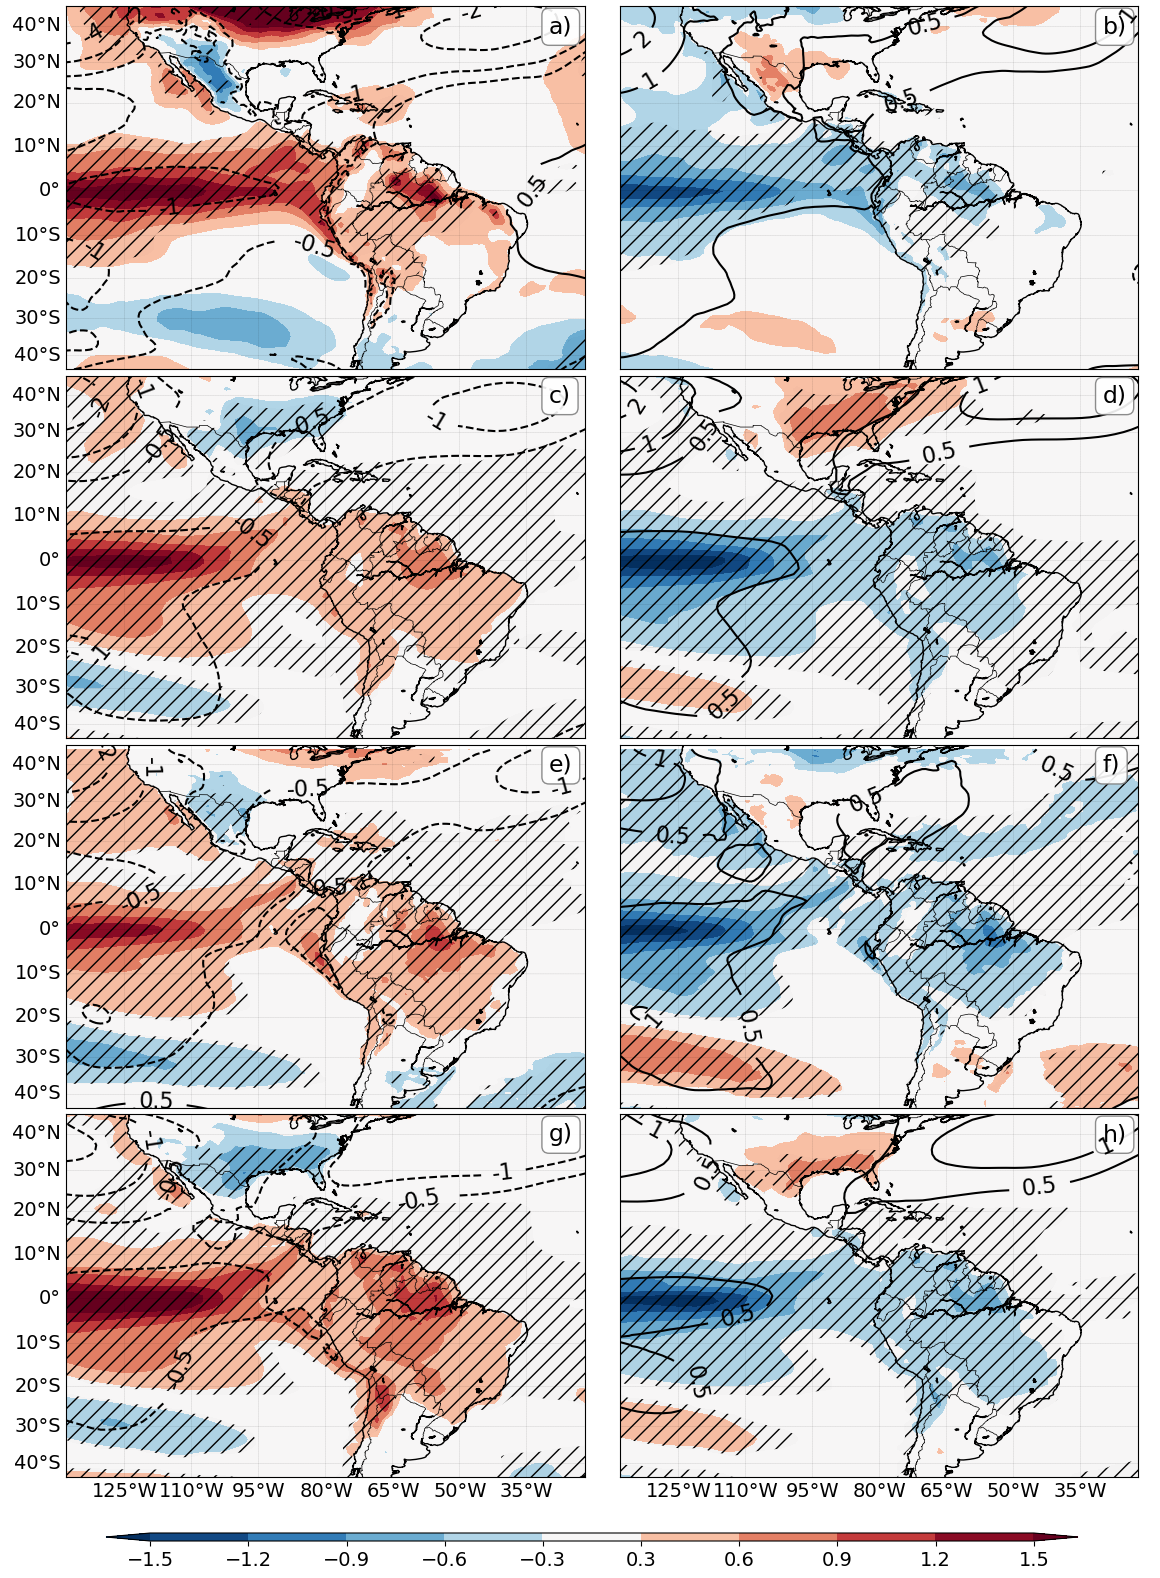
\includegraphics[width=0.81\linewidth]{figures/ensotemp_3}
\caption[ENSO teleconnections of temperature and SLP to the region of the AMS]{ DJF Temperature anomalies (colour contours in K) and SLP (line contours in hPa) during (a, c, e, g) El Ni\~no and (b, d, f, h) La Ni\~na events. Results are shown for (a, b) ERA-5, (c, d) UKESM1-hist, (e, f) GC3 N96-pi and (g, h) GC3 N216-pi. The hatched regions denote differences between ENSO phases and the climatological state with significance to the 99\% confidence level from a Welch t-test for the temperature field. }
\label{fig:10}
\end{figure}

The surface temperature and sea-level pressure (SLP) responses to ENSO events are shown in Figure \ref{fig:10} for HadGEM3, UKESM1 and ERA5 data during DJF, the season of strongest impact of ENSO events.
The characteristic warm anomaly during El Ni\~no events in the East Pacific Ocean does not extend as far east in the simulations as in the HadSST dataset or ERA5. In turn, the cold anomalies during La Ni\~na events in the Central Pacific are colder in the simulations than in ERA5. 
The teleconnection to southern North America, i.e., colder (warmer) conditions in southern (northern) North America during El Ni\~no events is relatively well simulated. For example, the simulated and observed teleconnection patterns to South America, e.g., the cold anomalies during La Ni\~na events in northern South America are well simulated. However, the low resolution simulations show a broader and stronger than observed negative response in southeastern US to El Ni\~no events. 

%The simulated teleconnection pattern to North America is better represented in GC3 N216-pi. % It is worth noting that the medium resolution simulations seems to simulate stronger El 

\begin{figure}[t!]
\centering
 %\noindent
 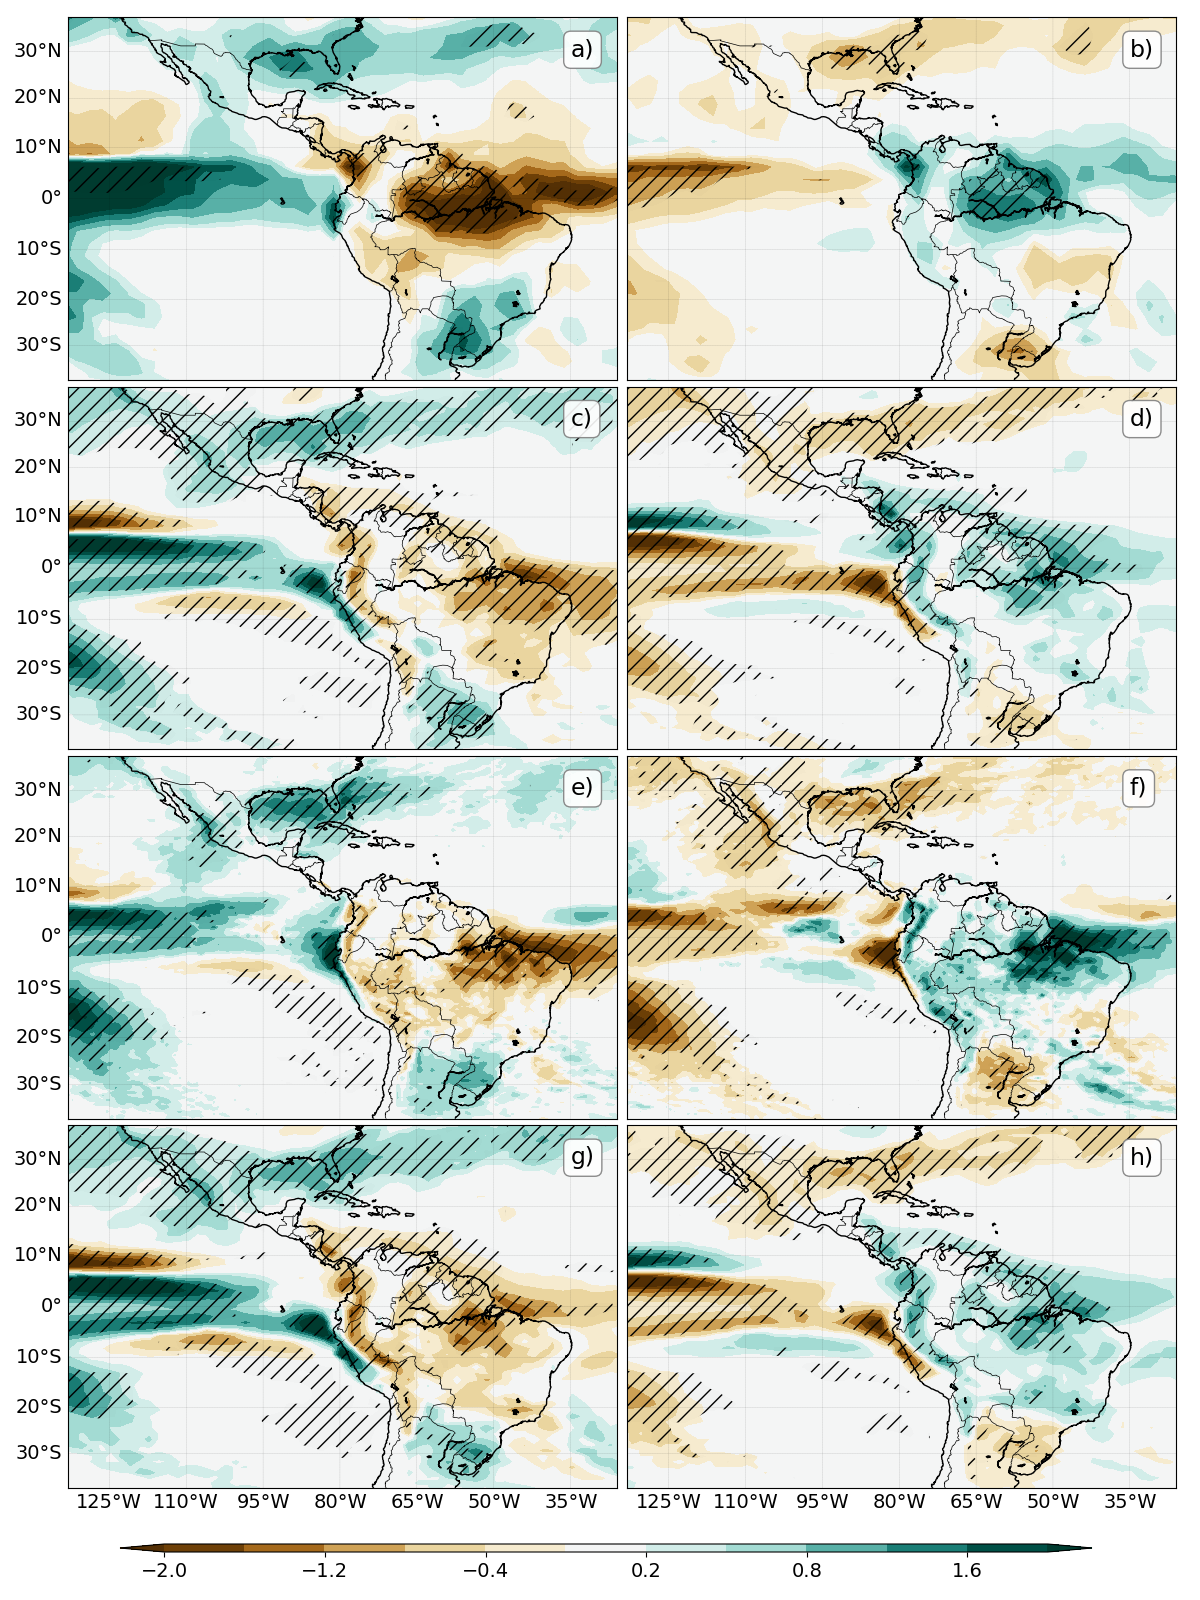
\includegraphics[width=0.81\linewidth]{figures/ensopr_3}
 \caption[ENSO precipitation teleconnections to the AMS]{As in Figure \ref{fig:10} but for the rainfall response [mm day$^{-1}$] using GPCP as the observational dataset.}
%\caption{ Precipitation  DJF response to (a, c, e, g) El Ni\~no and (b, d, f, h) La Ni\~na events in (a, b) GPCP, (c, d) UKESM1, (e, f) GC3.1 N96 and (g, h) GC3.1 N216. The hatched regions denote 99\% significance from a Welch t-test. }
\label{fig:11}
\end{figure}

The SLP response in the north Pacific and North America, known as the Pacific North-American pattern (PNA), is linked with a displacement of the subtropical jet affecting the eastward propagation of wave activity that reaches the North Atlantic  \citep[e.g.][]{bayr2019,jimenezesteve2020}.
During  El Ni\~no events, the Aleutian Low is strengthened in ERA5, with a strong SLP anomaly (-4 hPa) off the coast of California. The models show a similar but smaller SLP response in the same region.  El Ni\~no events events are associated with a negative phase of the North Atlantic Oscillation (NAO), with an opposite response for La Ni\~na events. While the models seem to be able to capture this response of the NAO, the simulated response is weaker than observed.   A sensible representation of the ENSO-NAO tropospheric teleconnection may be relevant to then simulate the effect of the NAO on Central American and northern South American rainfall \citep{giannini2000,giannini2004}.  




\begin{figure}
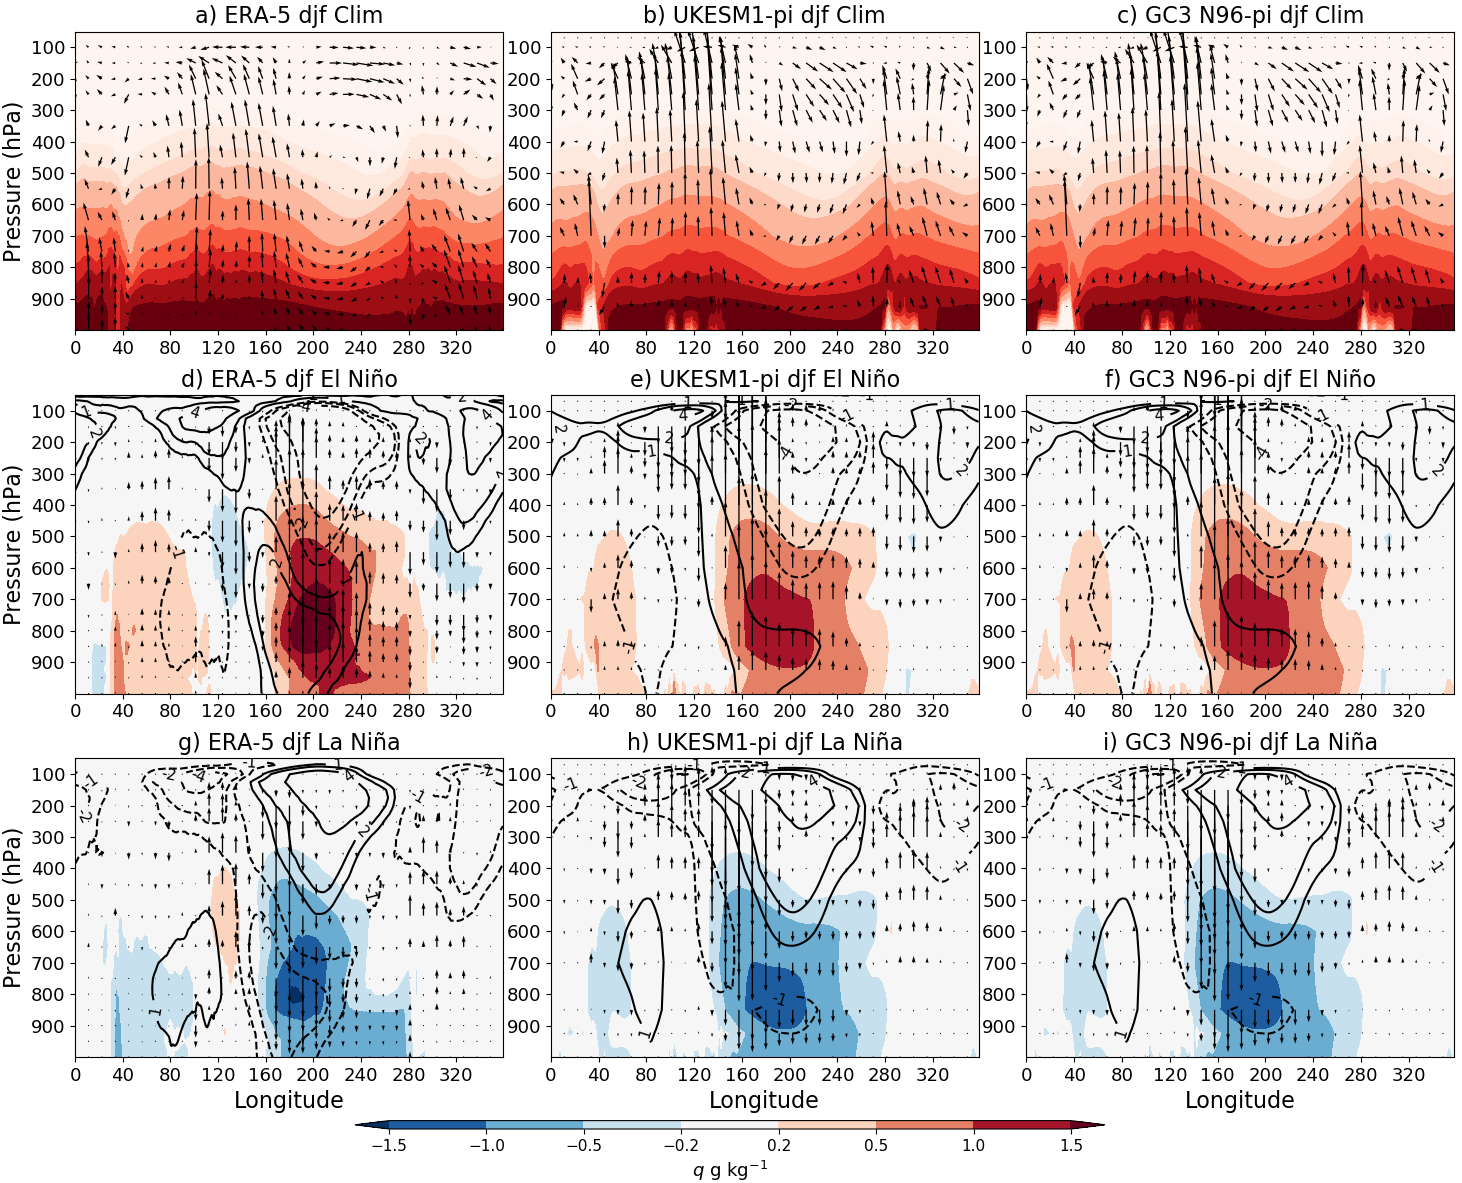
\includegraphics[width=\linewidth]{figures/walkerfinal}
\caption[Walker circulation anomalies associated with ENSO]{DJF Longitude-height Walker circulation anomalies of specific humidity (colour-contours), $\omega$ (vectors) and zonal wind (line-contours) during El Niño events (left) and La Niña events (right). Results are shown for ERA-5 (upper), UKESM-pi (middle) and HadGEM3 piControl (lower).}
\label{fig:swalker}
\end{figure}


The rainfall anomalies associated with ENSO events are shown in Figure \ref{fig:11}. Three regions in the AMS have a significant precipitation response to ENSO events in the observations and simulations.
In southern North America, rainfall increases (decreases) during El Ni\~no (La Ni\~na) events due to the effects of the PNA pattern on the subtropical jet, which influences the frequency and latitude of propagation of wintertime midlatitude disturbances which are the main source of rainfall in the region during the dry season \citep{vera2006,bayr2019}.


The GPCP dataset (Figure \ref{fig:11}a, b) shows significant boreal winter rainfall increases in southeastern US and the Gulf of Mexico during El Ni\~no events, and an opposite response to La Ni\~na phases. All the simulations reproduce this teleconnection rainfall pattern. 
The models also simulate the observed response in southeastern South America (SESA) of positive anomalies during El Ni\~no and negative anomalies during La Ni\~na events. This teleconnection to SESA is associated with the effect of ENSO on the sub-tropical jet in the Southern Hemisphere, the South Pacific and Atlantic Convergence Zones.

The anomalies in the Amazon show the strongest response to ENSO events in the observations. Significant positive (negative) rainfall anomalies during the negative (positive) phase of ENSO in northern South America are observed in GPCP. All the simulations show a very similar and statistically significant response. This teleconnection works through the coupling of ENSO with the Walker circulation \citep{vera2006,cai2019pantropical}, which is illustrated in Figure \ref{fig:swalker}. 

\begin{figure}[t!]
\centering
 %\noindent
 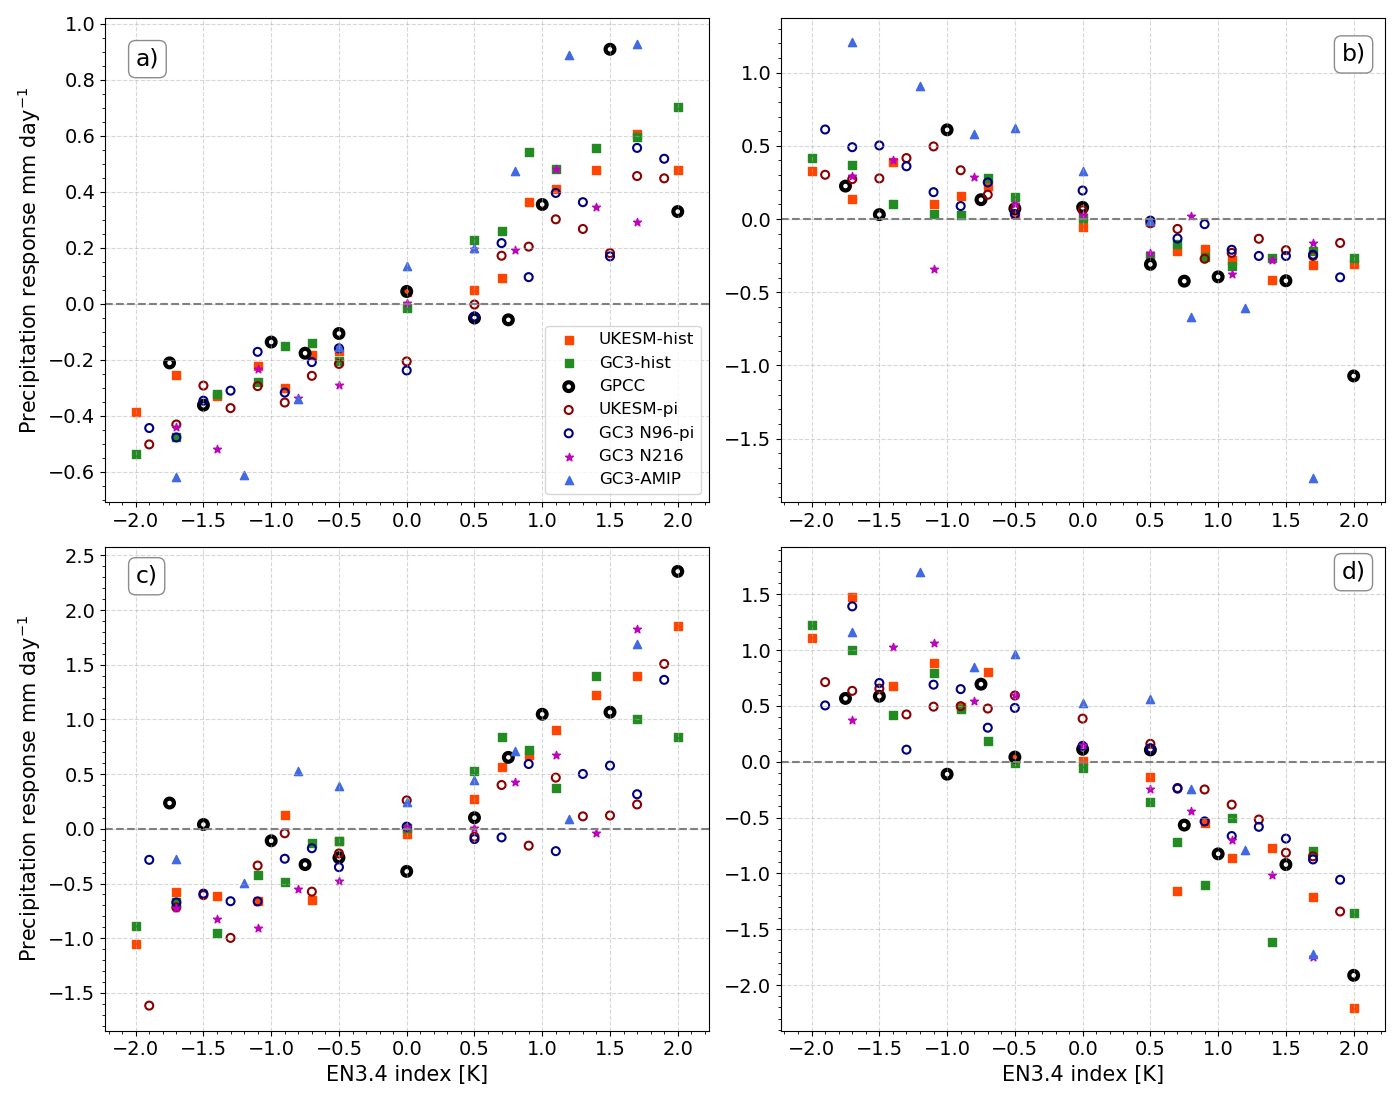
\includegraphics[width=\linewidth]{figures/fig_ensolinear}
\caption[Linearity of the precipitation response to ENSO events]{Precipitation response [mm day$^{-1}$] as a function of the El Ni\~no 3.4 index (see text) for (a) southwestern North America [20-37$^\circ$N, 112-98$^\circ$W], (b) Central America and southern Mexico [5-19$^\circ$N, 95-83$^\circ$W],, (c) Sout-Eastern South America [35-25$^\circ$S, 60-50$^\circ$W], and (d) the Amazon [10-0$^\circ$S, 70-45$^\circ$W]. The observation scatter points are from GPCC in the period of 1940-2013.}
\label{fig:12}
\end{figure}

The climatological Walker circulation during DJF shows strong ascent in the 100-160$^\circ$E and the 280-310$^\circ$E regions, which correspond to the maritime continent and South America (Figure \ref{fig:swalker}a). During El Ni\~no events, there is increased specific humidity throughout the lower troposphere in the Central and Eastern Pacific, associated with ascending motions in this region and negative low-level wind anomalies and positive upper-level wind anomalies (Figure \ref{fig:swalker}d). In other words, an eastward shift of the Walker circulation. The wind, vertical velocity and specific humidity anomalies are the opposite during La Niña events, indicative of a stronger Walker circulation, slightly shifted to the west. 
The models seems to broadly reproduce the observed changes to the Walker circulation during ENSO events (Figure \ref{fig:swalker}).


% The strongest simulated response is that of GC3 N96-pi, especially over eastern Brazil and the equatorial Atlantic Ocean. 





 Figure \ref{fig:12} shows the observed and simulated precipitation responses in four regions of the AMS to different magnitudes of ENSO events, by binning events for their magnitude of the EN3.4 index and the corresponding precipitation anomaly from the climatology in each region. This figure aims to show  the degree of linearity of ENSO teleconnections to the AMS.
While the observed response shows some degree of linearity for El Ni\~no events in South America (panels c, d), the majority of the observed responses, particularly to La Ni\~na phases, are not linear.

 However, the simulations show several signs of linearity. For instance, consider the historical experiments, UKESM1-hist and GC3 N96-hist, which show that the precipitation responses in southwestern North America, SESA and the Amazon increases roughly linearly as the magnitude of SST anomaly increases. In contrast, some other simulated responses, e.g. to La Ni\~na phases in South America in the piControl simulations, show signs of non-linearity.



\subsection{The role of ENSO flavours}
  
\begin{figure}[b!]
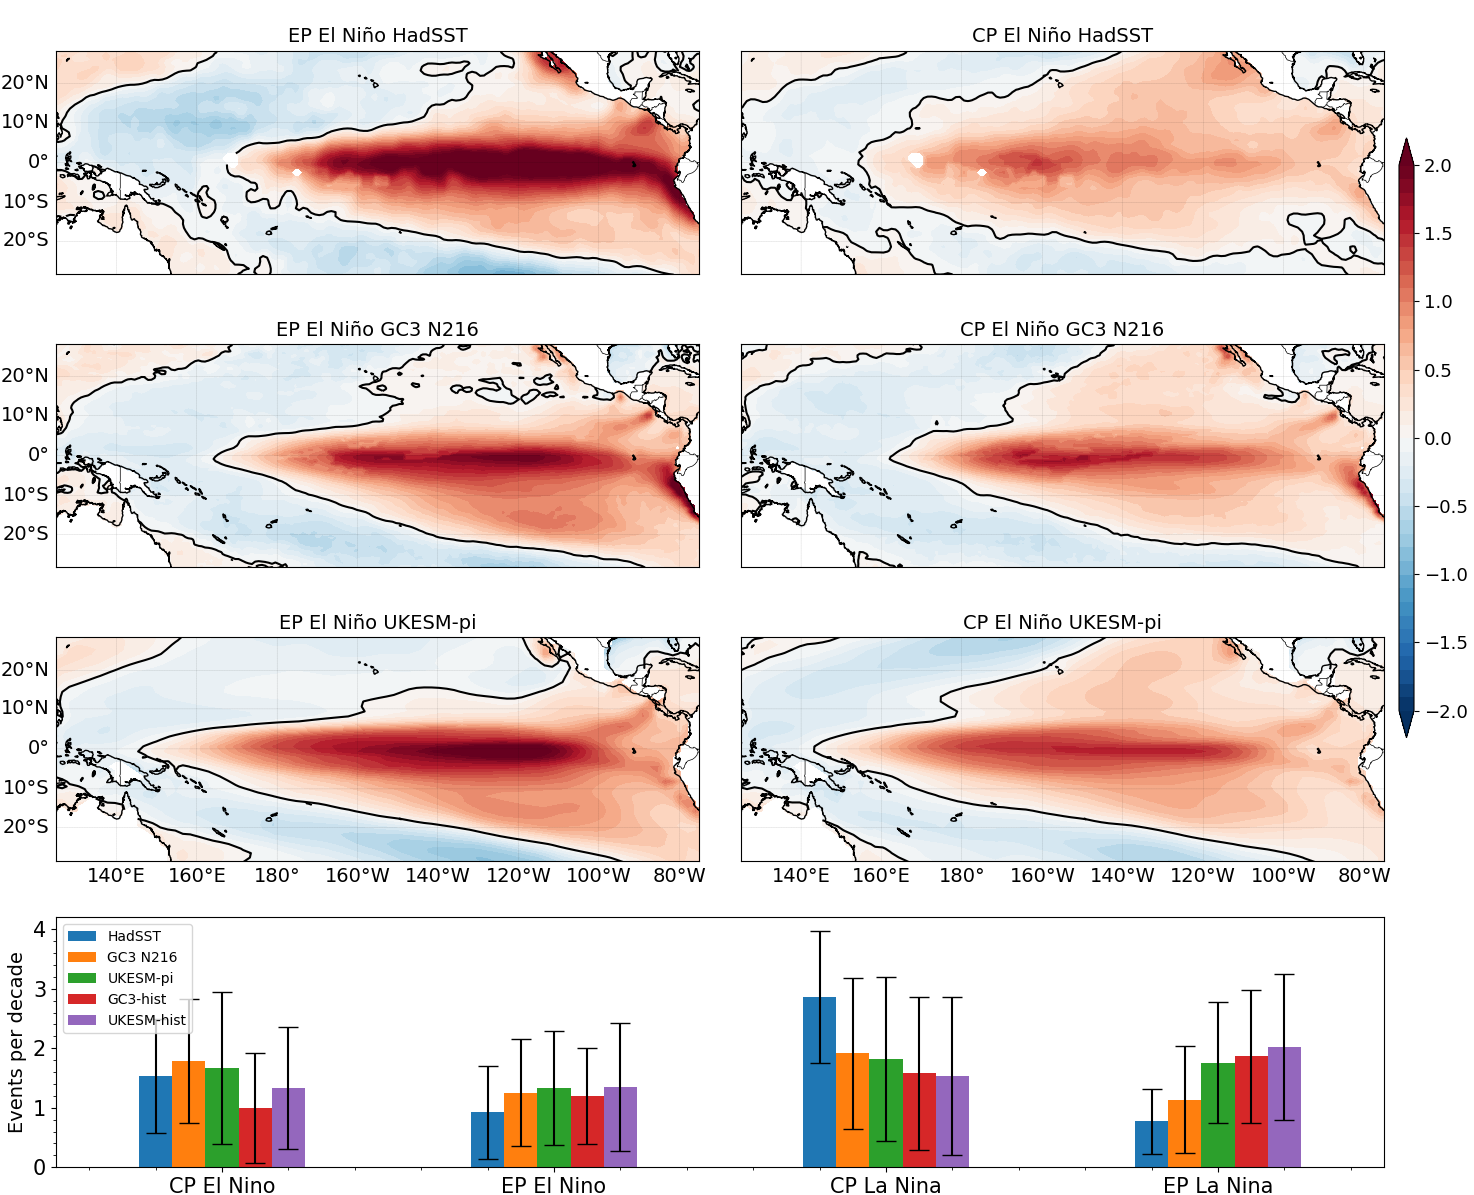
\includegraphics[width=\linewidth]{figures/epcpmap}
\caption[Diversity of ENSO SST patterns]{SST anomalies [K] for East Pacific (EP) and Central Pacific El Niño events in HadSST, GC3 N216 and UKESM piControl. EP (CP) events were defined where the E-index (C-index) was greater than 1. In the bottom panel, the frequency of events per decade (with standard deviation as error bar) is shown for HadSST and the simulations used in this study.
The E-index is computed from $(PC1-PC2)/\sqrt{2}$ and the C-index from $(PC1+PC2)/\sqrt(2)$.
}
\label{fig:s1}
\end{figure}


  
As described in section \ref{sub:lit_enso}, not all ENSO events are observed with the same SST anomaly pattern in the Pacific Ocean. These different SST patterns for each ENSO event are considered to be a source of non-linearity of ENSO impacts over South America \citep{sulca2018,cai2020}.
Principal component analysis has shown that ENSO events may be separated into two categories: Central Pacific (CP) and East Pacific (EP) events \citep{cai2020}, which highlight where the peak SST anomaly is found in the Pacific Ocean.
Figure \ref{fig:s1} shows that both UKESM1 and GC3 reasonably simulate the observed SST patterns associated with EP and CP El Niño events, although the simulations show CP SST patterns to spread further to the east than the HadSST dataset.
The simulations are also able to replicate very broadly the observed differences in the frequency of each event as CP La Niña events are more frequent than EP La Niña events, while the opposite is true for El Niño events.

\begin{figure}[t!]
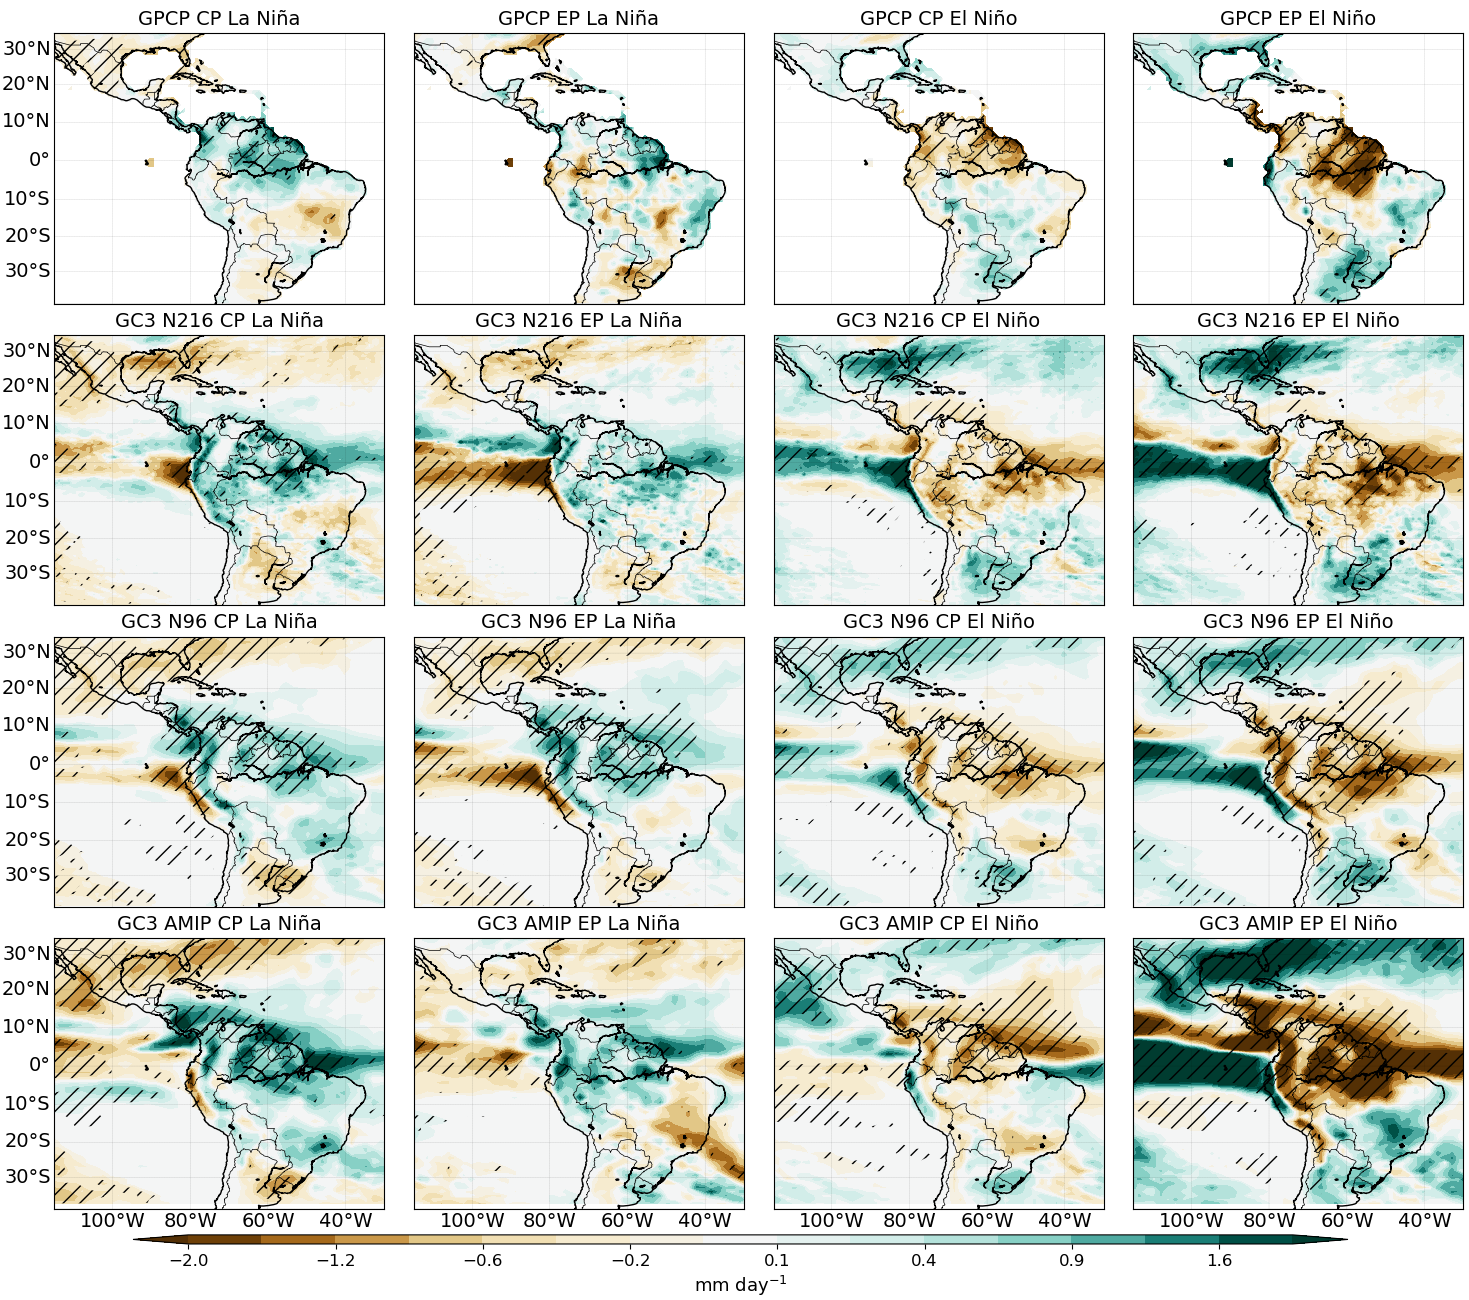
\includegraphics[width=\linewidth]{figures/cppranomalies_ff}
\caption[Precipitation anomalies to different ENSO flavours]{Precipitation anomalies in GPCC 1940-2013, GC3 N216-pi, GC3 N96-pi and GC3 AMIP for the four different types of ENSO events, as defined by \cite{cai2020}. Statistically significant anomalies (95\% confidence level) are hatched.}
\label{fig:senso}
\end{figure}  

Furthermore, Figure \ref{fig:senso} compares the precipitation anomalies for each type of ENSO event in observations with three simulations: GC3 N96-pi, GC3 N216-pi and GC3-amip. 
%The observations show significant precipitation responses differences in the Amazon, the Brazilian Nordeste and SESA between CP and EP events; however, these differences are less obvious in the coupled simulations (GC3 N96-pi, GC3 N216), but not in GC3 AMIP.
The observed precipitation response in the GPCC dataset to EP La Niña over equatorial South America is not significant and is smaller than the strong positive response to CP La Niña events in the same region. However,  the simulated response in GC3 N96-pi and GC3 N216 during La Niña events appears to be more independent of the type of event. In contrast, the GC3-amip simulations shows different magnitudes of responses to different types of La Niña events, in particular a positive, and significant, anomaly for CP La Niña events in the Amazon and weaker but not significant anomalies during EP events, which agrees with observations.

 The observed response to El Niño events in GPCC is also dependent on the type of event. EP EL Niño events show significant negative anomalies over the Amazon and positive anomalies over SESA whereas CP events only show significant anomalies (-1 mm day$^{-1}$) over northeastern South America. While the coupled models (GC3 N96-pi and GC3 N216) do show a stronger response to EP  EL Niño events than to CP events, the patterns of the response are very similar.
  In contrast, the response in GC3-amip agrees with observations, as stronger negative responses to EP El Niño events are observed in the Amazon compared to CP events in which the response is much weaker and is only significant in northeastern South America. In other words, GC3-amip agrees well with the observed non-linear teleconnection patterns whereas the teleconnections in the coupled models do not seem to depend  on the type of ENSO event.    

\subsection{A possible influence of the QBO on tropical ENSO teleconnections}

\begin{figure}[b!]
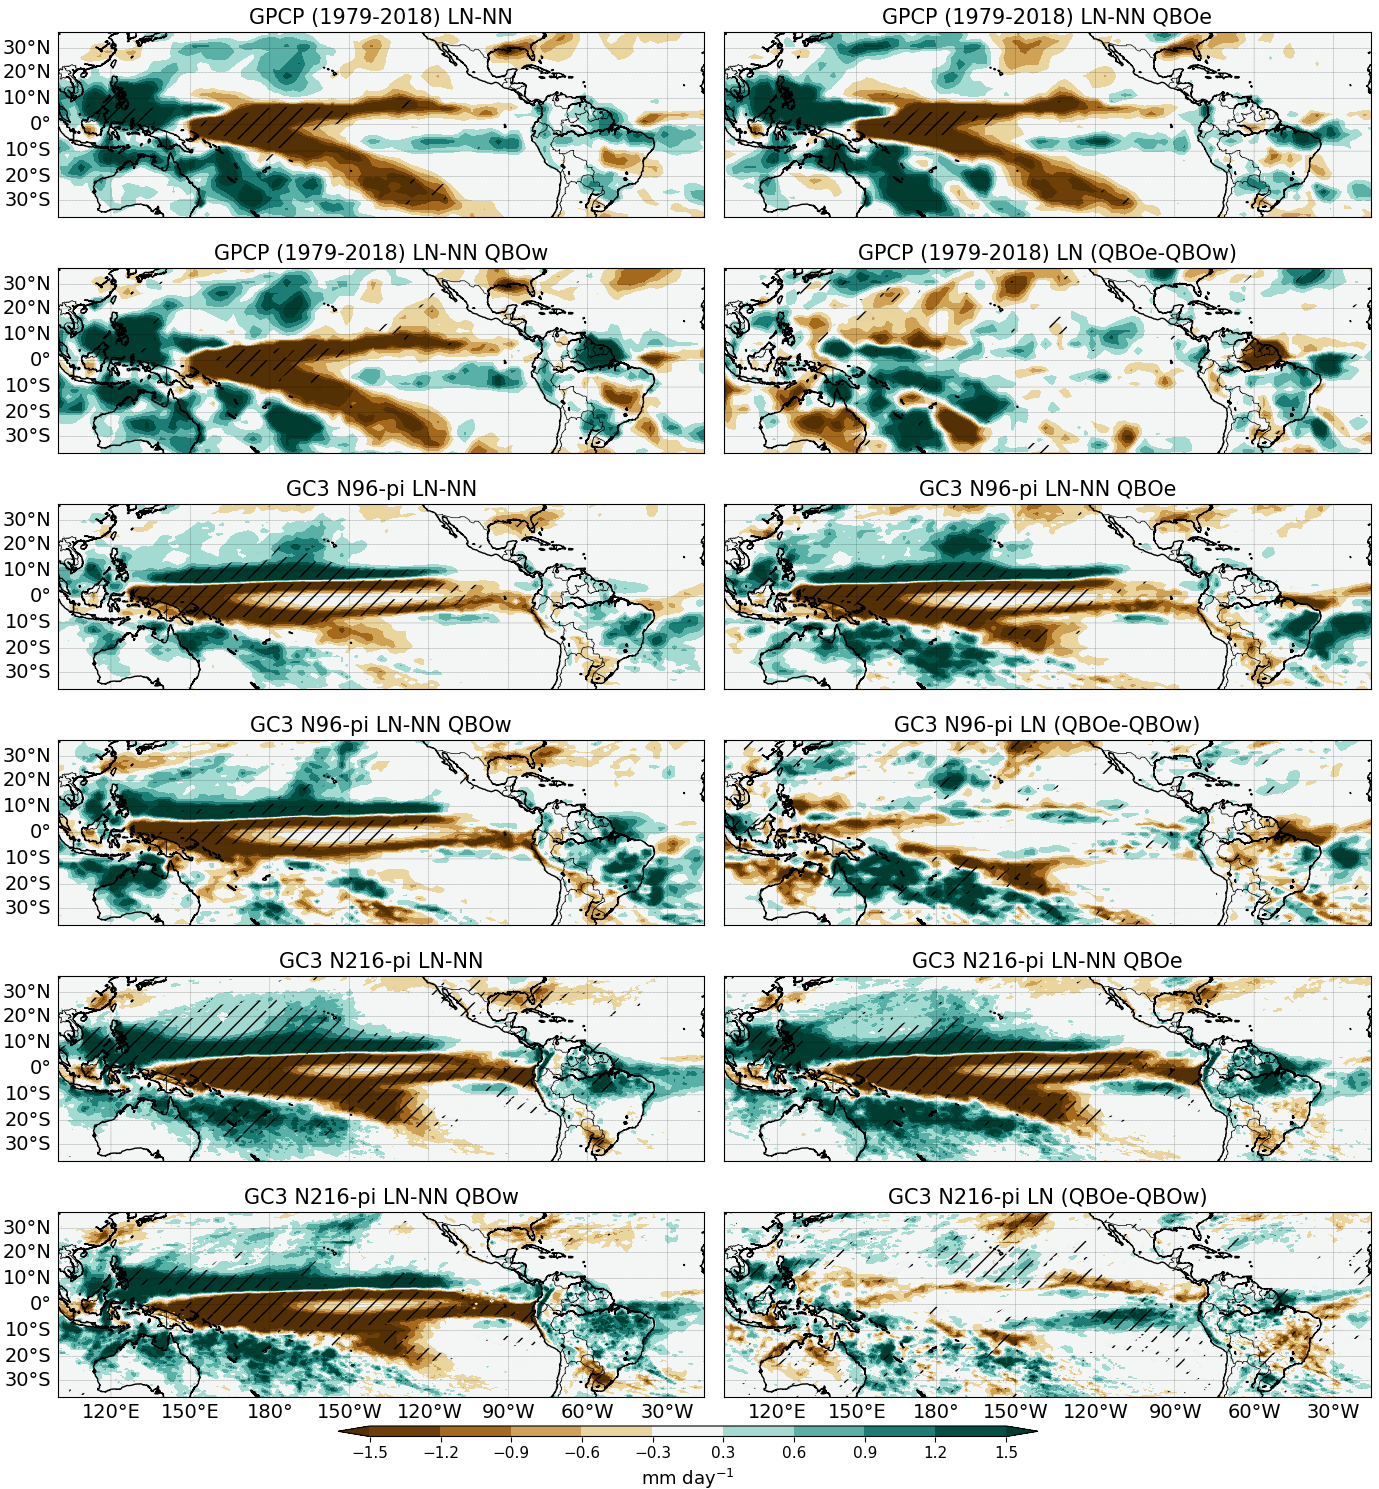
\includegraphics[width=\linewidth]{figures/trops_qbolnprfma}
\caption[Precipitation anomalies as a function of QBO and ENSO phases]{Composite precipitation differences during JFMA in GPCP (1979-2018), GC3 N216-pi and GC3 N96-pi between (top) La Niña and Neutral ENSO conditions. The two middle panels show a subset of the top panel, by separating the La Niña composite based on the phase of the QBO. The lower panel shows the differences QBO E-W during La Niña periods. Statistically significant anomalies (95\% confidence level) are hatched.}
\label{fig:qbopr_pis}
\end{figure}  

Section \ref{sq:qbolit} discussed the observational and modelling evidence of the effects on deep convection associated with the stratospheric quasi-biennial oscillation (QBO). In particular, some evidence suggest that the QBO may play a role to determine interannual variability of the Walker circulation and monsoons \citep{giorgetta1999,collimore2003,liess2012}. 

This section evaluates whether the simulations analysed in this chapter, as well as observations, show signs of an influence of the QBO on the AMS. 
In particular, the analysis aims to understand whether the QBO may be a source of non-linearity for the teleconnections of ENSO associated with deep convection and the Walker circulation. In all cases, the phases of the QBO were defined using a 70 hPa zonal mean zonal wind index, with a threshold of +2 m s$^{-1}$ for the westerly phase (QBOw) and -2 m s$^{-1}$ for the easterly phase (QBOe).

Composites of the precipitation response to La Niña (LN) events in Figure \ref{fig:qbopr_pis} show that the phase of the QBO may determine the strength and location of the teleconnection. 
While the precipitation difference in the western Pacific is relatively similar during QBOe than during QBOw in observations and simulations, the teleconnections to Australia, South America and the maritime continent are notably different depending on the QBO phase. 
In the GPCP dataset, the composite difference QBOe-QBOw during LN events suggests that the characteristic positive precipitation response during LN events in the Amazon, is largely associated with QBOw phases, whereas LN events during QBOe appear to have little effect over South America. 
A similar result is obtained for GC3 N96-pi. 


\begin{figure}[t!]
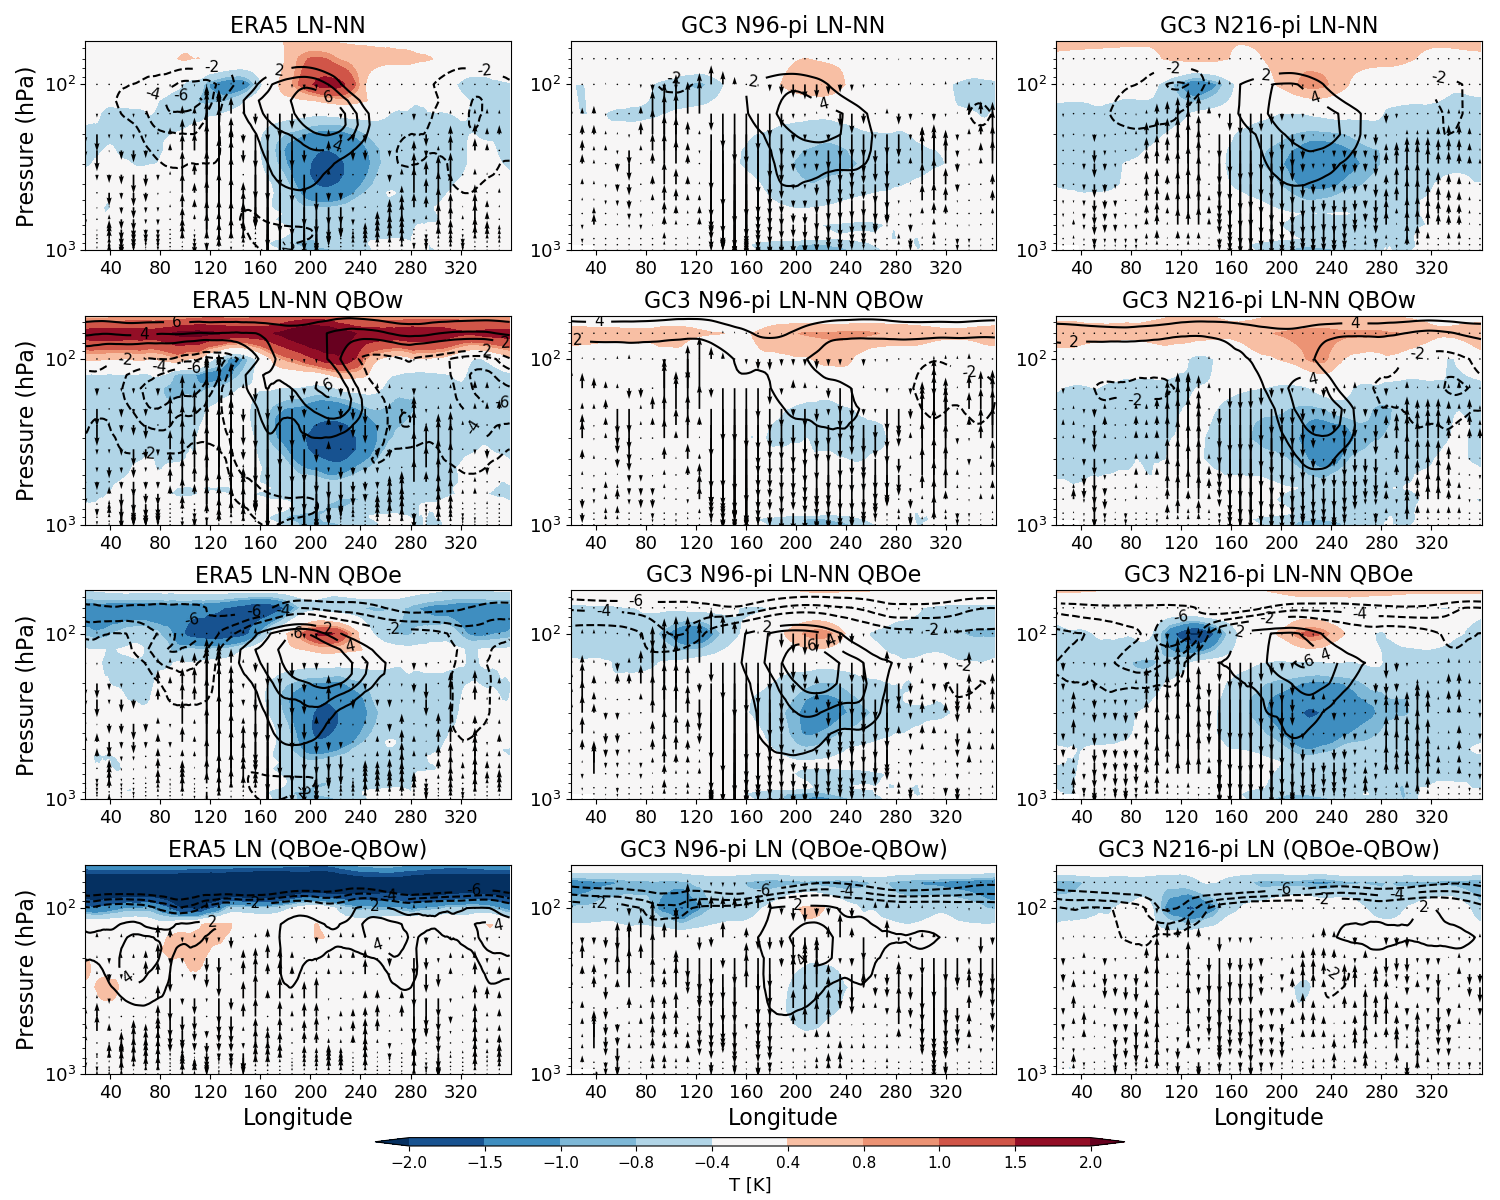
\includegraphics[width=\linewidth]{figures/walker_wqbo_jfma}
\caption[Walker circulation responses to La Niña under different QBO phases] {Longitude-height differences (JFMA) of equatorial (10S-10N) air temperature (color shading), zonal wind (contours) and vertical velocity ($\omega$ - vectors). The differences shown from top to bottom are between all La Niña (LN) periods and Neutral conditions (NN), between LN and NN during QBOw, LN-NN during QBOe, and the difference between LN events on different QBO phases (LN QBOe-QBOw). 
}
\label{fig:qbowalker_pis}
\end{figure}

These precipitation responses are further investigated by changes in the overturning circulation (Figure \ref{fig:qbowalker_pis}). As depicted in Figure \ref{fig:swalker}, La Niña events are associated with a westward shift in the Walker circulation with a strenghtening of the low-level easterlies in the Pacific Ocean. 
Figure \ref{fig:qbowalker_pis} shows that during LN the tropical troposphere cools and the UTLS region in the Central Pacific warms. These temperature anomalies are weaker in the simulations than in ERA5. 

The zonal wind anomalies in the upper-troposphere associated with LN events show different patterns and strengths during QBOw than during QBOe. The mean teleconnections during LN show positive upper-tropospheric anomalies above the Pacific Ocean,  but these anomalies are stronger during QBOe than during QBOw in ERA5 and the two simulations shown. In ERA5, most of the upper troposphere shows positive zonal wind differences in the QBOe-QBOw panel. 

There are three regions where ascending and descending motions are more greatly affected by LN events: the maritime continent, the Pacific Ocean and South America. The observed effect of the mean LN teleconnection is the following: anomalous ascent is seen in the maritime continent and in South America, in agreement with a stronger Walker circulation, whereas anomalous descending motions is observed in the Central and eastern Pacific associated with a westward shift of the Walker circulation. 


The effect of LN over ascending and descending motions is seemingly also affected by the QBO phase, according to the bottom panels of Figure \ref{fig:qbowalker_pis}. In ERA5 and the simulations, the anomalous ascent observed in South America during LN events is mostly associated with QBOw, whereas only small anomalous ascent is observed during QBOe. 
However, ERA5 disagrees with the simulations in the western Pacific region (140-180E), as the simulations suggest larger anomalous descent during QBOe than during QBOw, whereas in ERA5 these descending anomalies are larger during QBOw. 

A similar analysis was conducted to evaluate the effect of the QBO during the positive and the neutral phases of ENSO. These results are not shown because, although tentative suggestions were found that the QBO may play a role during these other phases of ENSO, there was little agreement between the models and ERA5/observations. Furthermore, the QBO representation in these CMIP6 models is biased in the UTLS region. In particular, the temperature signal associated with circulation of the QBO, most clearly seen in the bottom panels of Figure \ref{fig:qbowalker_pis}, is much weaker in the models. 

As suggested by the literature summarised in section \ref{sq:qbolit}, this temperature signal could be the key aspect of any effect of the QBO on deep convective systems, and as such, the evidence from a short record (ERA5) or models with key biases in possible processes involved presented in this chapter warrants both caution and more work. 
This topic will be investigated in the next chapters.

\section{Summary and discussion}



 This chapter assessed the MOHC models, HadGEM3 and UKESM1, in their pre-industrial control, historical and AMIP experiment contributions to CMIP6 with specific emphasis on the AMS and associated large-scale tropical circulation. These CMIP6 experiments allow the assessment of the effect of including Earth System processes or increasing resolution for representing regional monsoon rainfall. 
A schematic in Figure \ref{fig:13} shows the primary components of the AMS climate and summarises the main biases found in these simulations and this chapter.
%The study focuses on four regions in the AMS domain, the North American Monsoon, the MSD region of southern Mexico and Central America, southeastern Brazil and the Amazon.



Rainfall in the North American Monsoon was particularly well simulated by the models. The seasonal cycle, peak monsoon rainfall rates and timings of monsoon onset and retreat in the simulations agreed well with TRMM. The historical experiments overestimate the mean temperature in most of the Americas by 1.5 K, but particularly in boreal summer in southwestern North America (+4 K). Despite this warm bias, the temperature seasonal cycle is well represented by these models. 

  These results suggest model improvement of the simulation of the North American Monsoon from previous versions of the MOHC models \citep{arritt2000}, and most of the model cohorts of CMIP3 and CMIP5 \citep{geil2013}. For example, most CMIP5 models show a very wet bias during monsoon maturity whereas in all the experiments of this chapter this bias is less than 1 mm day$^{-1}$. However, these models continue to show biases during monsoon retreat as rainfall does not decrease as sharply as in observations after mid-September, which suggests a continued bias in the winter-time precipitation associated with cold-fronts \citep{adams1997}. Further research into the variability of the North American seasonality may be explored using these models given their skilfull representation of the seasonal cycle.

\begin{figure}[t!]
\centering
 %\noindent
 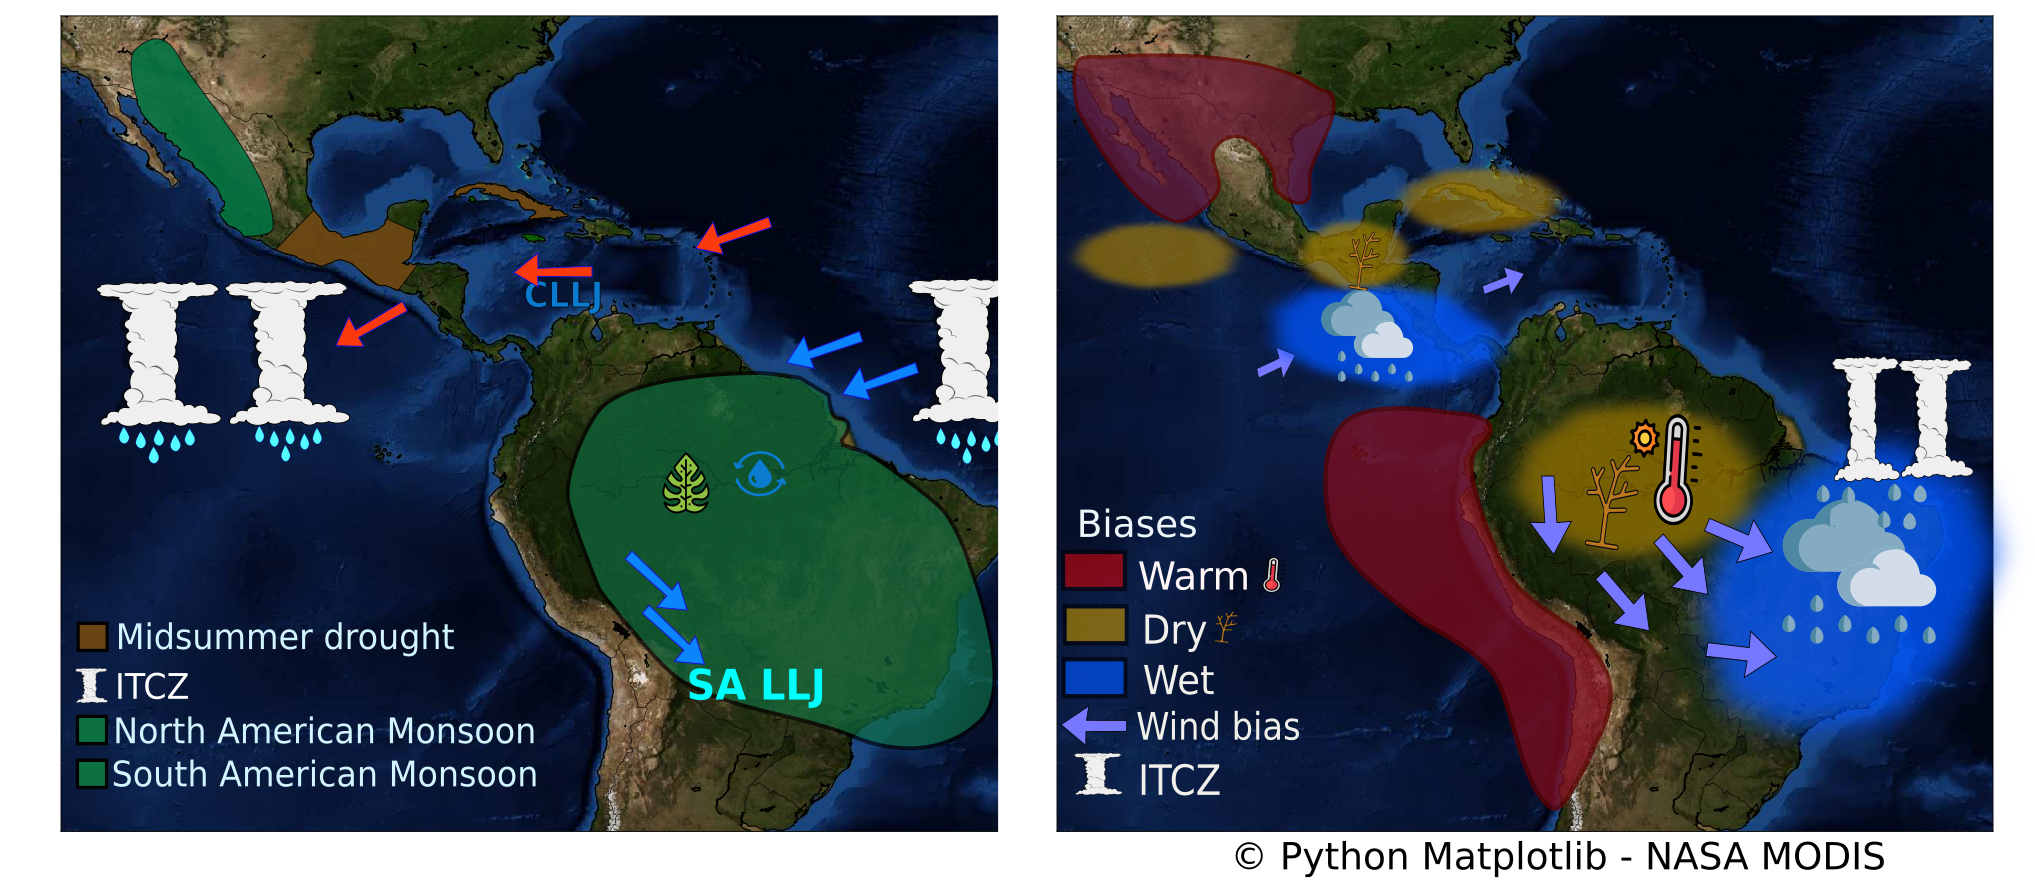
\includegraphics[width=\linewidth]{figures/drawing_d}
\caption[Summary schematic of biases in UKESM1 and HadGEM3]{Schematics of (a) the main features in the AMS and (b) the main biases in UKESM1 and HadGEM3. In (a) the boreal summer easterlies (red) and austral summer circulation (blue) are shown with the Caribbean and Bolivian Low-level Jets (CLLJ and BLLJ, respectively). In (b) the biases are shown for the respective northern and southern Hemisphere summers. The ITCZ bias in (b) refers to the southward displacement bias of the Atlantic ITCZ in the simulations.  }
\label{fig:13}
\end{figure}

    The Midsummer Drought (MSD) of southern Mexico and Central America is a regional feature of precipitation that most of the CMIP5 models had difficulty capturing, with the MOHC models being amongst the few exceptions \citep{ryu2014}. 
The MSD in UKESM1 and GC3 continues to be relatively well represented; however, the experiments analysed in this chapter showed various  differences in the timing and strength of the bimodal cycle when compared to observed gridded-datasets and ERA5.  
%The MOHC models were amongst the minority of CMIP5 models that simulated a seasonal cycle with a two-peak structure separated by a drier period \citep{ryu2014}. 

The models simulate a wetter-than-observed first peak of precipitation and a drier MSD period, therefore simulating a larger difference between the first peak and the dry period. While in observations this difference  between the first peak and the MSD period ranges between 2-3 mm day$^{-1}$, in the simulations the difference is closer to 6 mm day$^{-1}$.
Rainfall during the first peak has been too wet in these models since CMIP3, suggesting a persistent wet bias in this region, likely associated with the bias in East Pacific ITCZ also shown in this chapter and in recent studies \citep{ryu2014,mulcahy2018}. 
In contrast, the so-called second peak of precipitation, observed in late August, is simulated in close agreement with TRMM, except in the AMIP experiment, which has a wet bias of 2 mm day$^{-1}$ at this stage.

The skill of UKESM1 and HadGEM to simulate the MSD's bimodal regime of precipitation makes these simulations ideal to understand the mechanisms underpinning the MSD and why the MOHC models are able to represent a MSD regime but other models fail. Furthermore, section \ref{sq:litmsd} discusses several open questions regarding the mechanisms that cause the observed MSD. These simulations will then be used in future chapters to address the evaluate previous hypotheses of the causes for the MSD. 


The East Pacific ITCZ migration and position was shown to be relatively well represented by the models (Figs. \ref{fig:3} and \ref{fig:4}). However, the models showed an overestimation of boreal summer rainfall near the coast of Central America (Figure \ref{fig:8}). These biases are associated with an easterly wind bias at low levels, suggesting a bias in the flow from the Caribbean Sea into the Eastern Pacific  \citep{herrera2015,duranquesada2017}. 
The simulations also showed a biased Atlantic ITCZ that was displaced south of the observed ITCZ position during boreal winter (Figure \ref{fig:4}), particularly in the low resolution coupled simulations. 

In the Amazon, the simulations showed a warm bias (+2 K) during austral spring and summer, a bias that existed since CMIP5 \citep{jones2013}, and a colder than observed southeastern Brazil.
 These biases were linked with decreased cloud cover and less rainfall over the Amazon and more convective clouds and rainfall in southeastern Brazil (Figures \ref{fig:7} and \ref{fig:9}). 
The low cloud cover, warm and dry Amazon biases are intertwined with the low-level circulation from the Atlantic into the South American continent. The biases in the circulation during austral summer were observed as a northerly flow anomaly over the central and southern Amazon, a feature that has been associated with a stronger moisture transport away from the Amazon \citep{marengo2012,jones2017}. %The coupled simulations (Figure \ref{fig:7}) have a dry bias over the Amazon and a wet bias over southeastern Brazil. 


During the period of maximum rainfall rates in February, the simulations overestimate rainfall by 3 mm day$^{-1}$ in southeastern Brazil and underestimate rainfall in the Amazon by a similar rate. The historical experiments show a small drying response to historical forcing in the Amazon therefore slightly increasing the magnitude of this dry bias compared to the unforced piControl experiments.
The AMIP simulation with the SST biases removed improved the representation of the Atlantic ITCZ and the precipitation, cloud cover and temperature biases over the South American Monsoon.   The improvement in the circulation and precipitation biases in the AMIP simulation suggest that the origin of the dry Amazon bias are the biases in the Atlantic SSTs. 
%The simulated Amazon river basin also had shallower convection (higher 

  
The canonical teleconnection of  temperature, SLP and precipitation in the AMS to ENSO events are well represented in these models. For example, the simulated spatial patterns and strength of the positive (negative) precipitation anomalies observed in northern Mexico and Sout-Eastern South America during El Ni\~no (La Ni\~na) agree well with observations and reanalysis.
 Similarly, the teleconnection to the Amazon is well represented for both phases of ENSO, Despite relevant biases in the mean state of the South American monsoon discussed above. %in the region.  
 
ENSO teleconnections in these simulations were found to be approximately linear, i.e., the precipitation response is linearly related to the magnitude of the SST perturbation in the EN 3.4 region. These experiments also show signs of symmetric teleconnections as positive and negative phases produce the opposite and equivalent precipitation response in the AMS. In contrast to observations and the GC3 AMIP simulation, the precipitation response in the coupled models appears to be independent of the type or flavour of ENSO events, i.e., between Central and East Pacific events. The fact that these models show a reasonable representation of ENSO diversity in SST patterns but the models  do not replicate the observed non-linear dependence to ENSO events warrants further analysis.

The QBO appears to be a source of non-linearity for ENSO teleconnections to the Amazon. La Niña canonical teleconnections in the Amazon are characterized by a stronger ascent associated with a stronger Walker circulation. This teleconnection pattern occurs in observations and these simulations primarily during the westerly phase of the QBO, whereas the teleconnection during the easterly phase is much weaker and barely different from the climatological mean-state. Whether the stratospheric QBO poses such an important control of the main source of interannual variability (ENSO events) for monsoon rainfall in the Amazon merits a separate chapter of this thesis. 

The main biases (Fig. \ref{fig:13}) in these experiments are generally smaller in the medium-resolution GC3 N216 compared to the low-resolution experiments (N96), which suggests improved model performance with increased horizontal resolution.
In contrast, including Earth System processes in the UM model only affects the surface temperature response to historical forcing and not the dynamical biases that drive the precipitation and ITCZ biases. 
In short, the main dynamical biases in UKESM1 are very similar to those in GC3 N96 as these two models  share the same dynamical core; only when resolution is increased are these biases reduced notably. 

A noteworthy difference between UKESM1 and GC3 is that warming over the historical period in Mexico and the Amazon is higher in UKESM1 than in GC3. In general, UKESM1-hist shows a stronger temperature response to forcing than GC3 N96-hist, as UKESM1 has been reported to have a  greater climate sensitivity than GC3 N96 \citep{andrews2019,sellar2019}.  This differential warming may be a consequence of the land-use change in these regions playing a role in the UKESM1 representation of soil-atmosphere feedbacks. %In short, the main dynamical biases, such as the biased austral summer circulation in South America, are only improved when the resolution is increased, whereas the addition of Earth System processes does not improve dynamical biases that influence the characteristics of rainfall in the AMS. %This results suggets that improvement in monsoon representation is associated with resolution


%The results of this study showed that the medium resolution (GC3 N216) simulation improved upon some of the biases of the lower resolution simulations, such as most of the precipitation biases. %
The improvement in the medium resolution simulation compared to the low-resolution simulations may  be attributed to the improved dynamics of the ocean or the atmosphere. %associated with relying less on model parametrisations.
For example, the Atlantic ITCZ biases have been shown to be directly affected by processes in the convective scheme \citep{bellucci2010}, such as the treatment of entrainment and moisture-cloud feedbacks \citep{oueslati2013,li2014}. 
The resolution of the ocean model has been shown to impact the eddy heat flux parametrisation and the associated heat uptake and transport of the ocean  \citep{kuhlbrodt2018}. The improvement in the Atlantic SSTs and ITCZ and the associated dynamics in GC3 N216-pi also improves the associated circulation biases and moisture transport in the South American Monsoon. In other words, the oceanic resolution may play an important role in the cross-equatorial heat and moisture transport which largely control the SST gradients over the equatorial Atlantic. The SST biases in the Atlantic are likely the dominant factor to accurately simulate the spatial distribution of rainfall in South America.

%These CMIP6 simulations of HadGEM3 and UKESM1 show some signs of model improvement, particularly in the North American Monsoon and may be used to better understand the response to current and future response to anthropogenic forcing. Furthermore, several aspects of the climate of the AMS that are well simulated by these models, such as a good representation of the MSD and a resonable representation of ENSO diversity, may suggest further use of these simulations to address outstanding questions of climate variability in this region across different temporal scales.



\chapter{\label{ch:5-wvt}A wavelet transform method to determine monsoon onset and retreat from precipitation time-series}

This chapter describes a new method to determine monsoon onset and retreat timings using wavelet transform methodology applied to precipitation time-series at the pentad scale. 
The use of the method is illustrated for the North American Monsoon and the Indian Monsoon using four different precipitation datasets and climate model output. 
An extension of the method is used to identify the timings and strength of the Midsummer Drought of southern Mexico, Central America and the Caribbean. 
The advantages and shortcomings of the method are discussed at the end of the chapter.

\section{Introduction}

The timing and strength of the rainy season are key aspects of the climate of monsoon regions as the onset or start and the retreat or end of the monsoon rainfall greatly influences sectors such as agriculture \citep{sultan2005,Gadgil2006,jain2015,harvey2018} and water management \citep{turner2012,bussman2016}.
Scientific and societal motivation has led climate and weather research to objectively determine  onset and retreat dates for purposes such as the characterisation of variability and trends, and forecasting \citep[e.g.][]{kitoh2006,cook2009,picher,nieto2011,htway2011}. 

For this reason, a wide range  of methods exist to diagnose the onset and retreat dates from a number of variables and datasets.
\cite{bombardi2019} provides a recent review of these methods and highlights the technical differences and purposes of each. Methods can be divided into those that evaluate monsoon onset and retreat on a regional scale \citep[e.g.][]{webster1992,fasullo2003,garcia2013}  or at a local or grid-box scale \citep[e.g.][]{liebmann2001interannual,cook2009}. 

Threshold methods are the most commonly used local-scale methods that typically diagnose onset and retreat from a precipitation time-series \citep{bombardi2019}. 
These methods evaluate the accumulated  \citep{liebmann2001interannual} or daily/pentad-mean rainfall rates \citep{geil2013} and determine the onset and retreat dates when the time-series exceeds or falls below a pre-defined value (threshold) for a given amount of time (persistence). The persistence parameter aims to decrease the effect of noise of precipitation in the calculation. The threshold parameter can be a statistical measure of the seasonal cycle such as the total annual mean rainfall \citep{arias2012}  or tuned to a specific dataset \citep[e.g.][]{geil2013}.

%The parameters for threshold methods vary distinctly from study to study, first, because the wet and dry seasons in each monsoon region have different timings, strengths and dynamical features \citep{wang2017}. Secondly, parameters may vary due to differences between the datasets used, e.g., in horizontal resolution, can cause differences in the climatological seasonal cycle of rainfall or the mean rainfall rate, requiring different threshold and persistence parameters for each dataset.% which means that the implementation of threshold methods in different datasets also requires normalization or statistical treatment of the threshold and persistence parameters.

%Furthermore, within a given monsoon region,  e.g., in the South American Monsoon, several methods are used for different purposes depending on the temporal and spatial scales of interest \citep[see e.g.][]{liebmann2001interannual,marengo2001,nieto2011,carvalho2011,garcia2013}.
%Finally, 

In other words, for a given purpose each threshold method is tailored to a monsoon region using a specific dataset and a specific variable. This characteristic of the threshold methods poses various shortcomings.  
 Firstly, practical shortcomings of the threshold methods, particularly rigid thresholds, include false hits \citep{moron2014interannual} or some years not meeting the threshold and persistence criteria \citep{arias2012} requiring further relaxation of the parameters. Secondly, given that threshold methods are tailored to a specific dataset in a given region, statistical corrections are needed to implement the same threshold method in a different dataset or in another region. 
% Furthermore, the conclusions of most analyses of threshold methods arise from the output of one single-method and one single dataset. These studies would benefit from the input of a second independent method to confirm the results. However, due to the differences between regional monsoons most techniques are not suitable to be used in other regions.
 
 The Coupled Model Intercomparison Project (CMIP) assessments of monsoon onset and retreat typically use precipitation threshold methods due to the lack of high temporal or vertical resolution output from all models to estimate vertically integrated quantities required for some methods \citep[e.g.][]{geil2013,zou2015,jamoon2020}. Threshold methods have multiple shortcomings for CMIP assessments as the persistence and threshold parameters are tuned for observations with a specific seasonal cycle but models have a range of biases in the seasonality, magnitude and spatial distribution of rainfall \citep{pascale2019,garciafranco2020}. 
The use of pre-defined threshold values may also not be suitable to compare different model experiments with changes in forcing where the climatological mean rainfall or the seasonal cycle may change within the model run.
These shortcomings are relevant because a proper diagnosis of the seasonal cycle in CMIP assessments is key to understand and diagnose current and future changes to monsoon seasonality as a result of greenhouse forcing \citep{zhou2016,wang2017}. 

%The observational or model-based analysis of the monsoons as a global phenomena also require a systematic approach to determine onset and retreat dates  that is not tailored to any specific region \citep{zeng2004globally}. For example, projects such as the  Global Monsoons Model Inter-comparison Project (GMMIP), which is part of CMIP6, may benefit from broader and more systematic methods to be used across models and monsoon regions \citep{zhou2016} and particularly methods that can be implemented with standard output from modelling centres. These systematic or large-scale methods may also be relevant in the evaluation of trends in the timings of the rainy season on hemispheric or global scales in observations and models \citep{zeng2004globally,zhang2008global}.  

The objective diagnosis of shorter time-scale rainfall variability, such as bimodal regimes and active and break phases of a monsoon, also requires methods that can separate relatively drier and wetter periods within the rainy season. For example, for the MSD of Central America and the Caribbean (section \ref{sq:litmsd}) the objective determination of the strength, spatial distribution and robustness of the bimodal signals is not straightforward. For example, the global method used in \cite{bombardi2019} fails to diagnose the region of southern Mexico, Central America and the Caribbean as a bi-modal regime. 

The majority of existing methods to diagnose bimodal signals in the MSD region use geometric or statistical measures of the monthly-mean rainfall that measure the difference between the months of maximum rainfall and the drier months.  
However, this approach fails to capture the shorter-scale changes that have been shown to occur in both observations and model data, as the MSD does not start or end exactly on given calendar months \citep{magana1999,garciafranco2020}.  \cite{zhao2021} review and compare several methods to detect and measure the MSD, finding that using monthly-mean data and prior assumptions of the dates of the first and second peaks can lead to errors.  %but can also introduce biases when determining the spatial variability of the MSD \citep{zhao2021}.

Only a handful of methods exist that can determine the characteristics of the MSD in Central America on sub-monthly timescales. \cite{anderson2019multiscale} analysed the pentad-mean time-series from the   Climate Hazards Infrared Precipitation with Stations (CHIRPS) dataset. After a double temporal smoothing of the time-series, \cite{anderson2019multiscale} determined the MSD timings through a threshold method with parameters tailored to the CHIRPS dataset.
In turn, \cite{zhao2020} used daily-mean time-series and determined the two-peak structure through linear-regression analysis.
However, more general methods that may be applied to multiple datasets on the daily-mean scale could provide useful to understand variability and trends in the seasonality of precipitation in the region.


In short, multiple methods exist to diagnose monsoon onset and retreat as well as bimodal signals, each with various parameters fit for different purposes, but these methods present shortcomings for studies that compare results from multiple datasets or investigate model experiments where the climatological rainfall and the seasonal cycle are non-stationary.
%Similarly, studies that investigate the impact of decadal modes of variability \citep[e.g.][]{arias2012}, greenhouse warming \citep[e.g][]{geil2013} or general trends \citep[e.g.][]{Sahana_2015} rely solely on the output of one single method whereas the use of two or more methods may help to test the sensitivity of their results to the chosen method and parameters. 
Both the objective determination of monsoon onset and retreat and the timings of bimodal regimes require a method that can analyse temporal changes to precipitation on several scales and that can be used on any gridded dataset. 



  The purpose of this chapter is then to present an objective approach that is more portable across datasets, regions, less prone to false-hits and robust for various purposes.
This chapter introduces a wavelet transform method to determine monsoon onset and retreat dates using pentad-mean precipitation time-series.  Wavelet algorithms have been extensively used in atmospheric research for multiple purposes, such as the detection of the boundary layer height \citep[e.g.][]{brooks2003}, as well as to analyse time-frequency features of a signal \citep[e.g.][]{whitcher2000,dimdore2021}. In fact, \cite{allen2017} used a wavelet analysis to determine monsoon onset and retreat using daily OLR data. The remainder of this chapter is organised as follows: section 2 describes the methods and datasets. Section 3 shows the results of applying the method to the Indian and North American Monsoons and the MSD. Section 4 summarises the method and discusses the results.
%The method is constructed such that the determination of monsoon onset and withdrawal dates is less sensitive to the characteristics of the time-series, i.e., the characteristics of the seasonality of each monsoon  or of a given observational dataset. Furthermore, the method is expanded to characterise bimodal regimes which is illustrated for the MSD of southern Mexico, Central America and the Caribbean.



\section{Data}

\subsection{Precipitation datasets and reanalysis data}

This chapter uses three gridded precipitation datasets described in chapter \ref{ch:3-methods}: the TRMM v7 3B42, the CHIRPS, and the CMAP datasets.
These three precipitation datasets are merged products, TRMM and CMAP mainly use microwave satellite measurements complimented by several other sensors and calibrated with rain-gauge data whereas CHIRPS uses several products from TRMM, as well as high-resolution station data. These datasets also differ in their end-product horizontal resolutions.

The precipitation output from the latest ECMWF reanalysis, ERA5, is used, which has been shown to exhibit a relatively good representation of the temporal characteristics of rainfall in the AMS in chapter \ref{ch:4-ams}. 
Other variables from ERA5 used to diagnose changes to the circulation associated with monsoon onset were daily-mean geopotential height at 500 hPa and wind speed ($\vec{u}$) at several vertical levels. 

\subsection{Model data}


Daily precipitation data from the CMIP6 archive are used and retrieved from: \url{https://esgf-index1.ceda.ac.uk/projects/cmip6-ceda/}, to illustrate the method using standard climate model output.
In particular, we use results from the piControl and historical simulations of HadGEM3 GC3.1 and UKESM1, described in chapter \ref{ch:3-methods}.
The daily precipitation data were converted to pentad-scales.

%Table S1 provides a summary of the experiments used and the acronyms of each experiment for each model \citep{menary2018,gc3pi,n216pi,sellar2019}.
%HadGEM3 GC3.1 was run at two horizontal resolutions, N96 and N216 for the pre-industrial control experiment (Table S1). UKESM1 differs from HadGEM3 by representing Earth System processes, such as interactive ocean biogeochemistry and atmospheric chemical interactions \citep{sellar2019}.
%The pre-industrial Control experiments use constant forcing estimated for 1850 whereas the historical experiments aim to represent time-varying greenhouse emissions, volcanic eruption and solar signals in the historical period (1850-2014) \cite{eyring2016}. %and other forcings. 
%These simulations were recently evaluated in the North American Monsoon and the MSD region, showing a good representation of the seasonal cycle in these regions \citep{garciafranco2020}.

\section{The wavelet transform method}

\defcitealias{geil2013}{G13}
\defcitealias{arias2012}{A12}

Wavelets are band-limited wave-like functions with specific mathematical properties that include a finite energy and zero-mean \citep{whitcher2000,addison2017}.
The wavelet function is defined using two parameters, a dilation (a width or temporal scale) and a translation (centroid in time/space).

Wavelet transforms are the result of the inner product (convolution) of a wavelet function with  a time-series or a signal \citep{addison2017}. 
The wavelet transform (WT) can be thought of as a local comparison between the wavelet function and the observed signal for different frequencies.
The information provided by a WT largely depends on the characteristics of the wavelet function, such that different wavelet functions are used for different purposes \citep{addison2017}. For the purpose of finding the onset and retreat dates, the wavelet based on the Haar function is useful as this wavelet finds sudden changes in a signal, in a way acting as a temporal filtering of the data \citep{addison2017,brooks2003}. The Haar wavelet is defined as the non-continous piece-wise function:

\begin{equation}
\psi \bigg(\frac{t-b}{a}\bigg)=
\begin{cases}
      1 & b\leq t < b+\frac{a}{2} \\
      -1 & b-\frac{a}{2} \leq t < b \\
      0 & elsewhere,
   \end{cases}
   \label{eq:haar}
\end{equation}
%
\noindent where $a$ is the dilation coefficient, $b$ is the centre of the wavelet or the translation coefficient and $t$ is the time coordinate.

The wavelet covariant transform is then the inner product of the Haar wavelet with a timeseries \citep{brooks2003}, as follows:

\begin{equation}
W_f(a,b)=\frac{1}{a}\int_{t_i}^{t_f}pr(t)\psi \bigg(\frac{t-b}{a}\bigg) dt,
   \label{eq:wf}
\end{equation}

\noindent where $pr(t)$ is a time-series of precipitation, either on daily or pentad scales and $W_f(a,b)$ is the matrix of the covariant transform and $t_i$ and $t_f$ are the start and end time-points. No statistical treatment, normalization or anomaly, \textit{a priori}, is calculated on the precipitation time-series $pr(t)$ so the units of $W_f$ are the same as the precipitation time-series (e.g. mm d$^{-1}$).

 Monsoon timings can be observed as sharp changes to precipitation, i.e., rainfall sharply increases at onset and sharply decreases at retreat. However, measuring these changes can be difficult since precipitation time-series are typically noisy. The Haar wavelet is useful in these cases for signal detection since the WT is interpreted as  gradients across different temporal scales and can smooth out the high-frequency variability using sufficiently large dilation scales. 
  In other words, the wavelet covariant transform ($W_f(a,b)$) filters the time-series $pr(t)$ using a temporal scaling of $a$, or measures gradients on a scale $a$ for each time-step ($b$).
  
  \begin{figure}[t!]
\centering
 %\noindent
 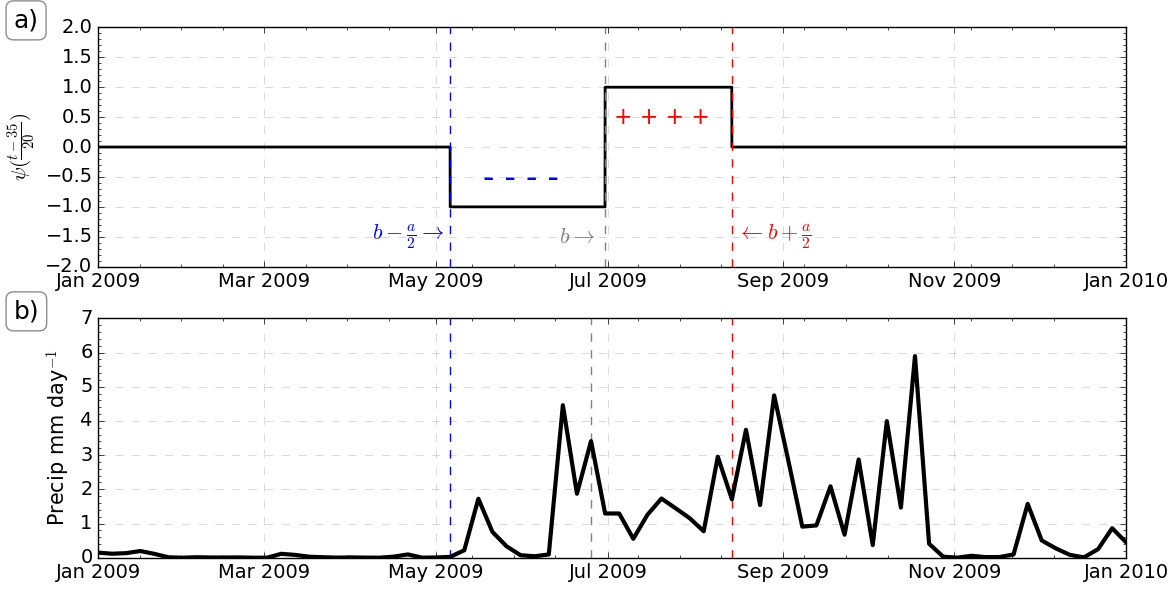
\includegraphics[width=\linewidth]{figures/wav1.png}
\caption[Haar wavelet exmaple]{ (a) Haar wavelet at a dilation $a=20$ and translation $b=35$, which is the 35rd pentad around June 22. The positive and negative parts of the wavelet are highlighted in red and blue, respectively. (b) CMAP precipitation in 2009 in the North American Monsoon [20-27$^\circ$N,110-103$^\circ$W]. }
\label{fig:wvt_f1}
\end{figure}


\begin{figure}[t!]
\centering
 %\noindent
 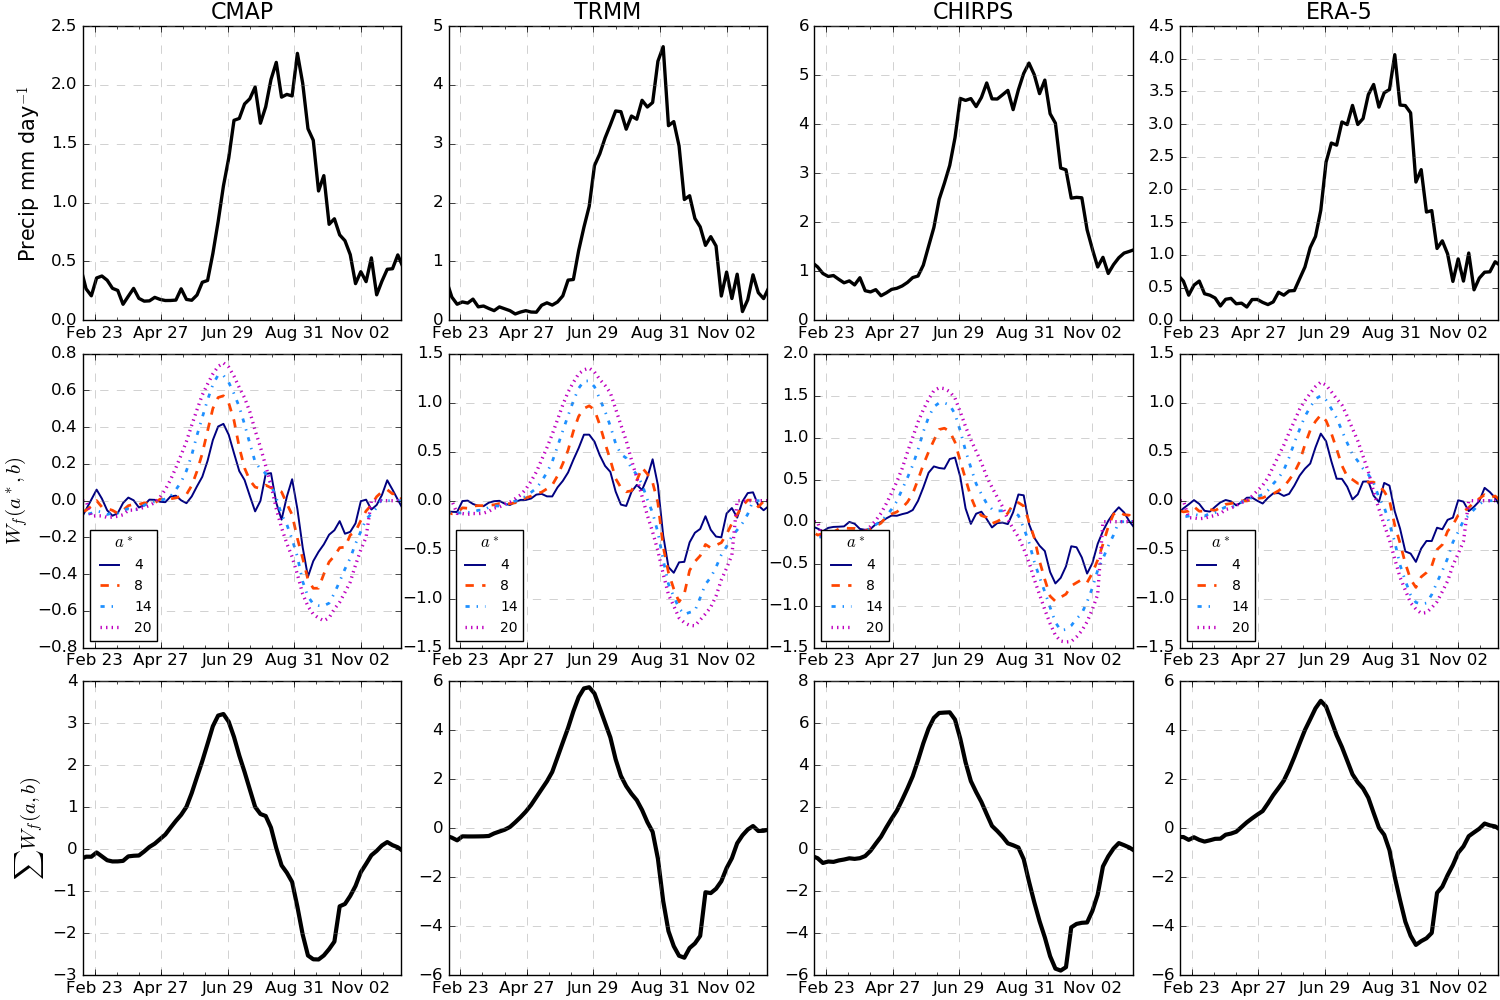
\includegraphics[width=\linewidth]{figures/wav_paperfig2.png}
\caption[Wavelet transform coefficient in North American Monsoon]{ (upper) Climatological pentad-mean precipitation in four different observational datasets in the North American Monsoon [19-35$^\circ$N,110-103$^\circ$W]. (middle) The wavelet transform coefficients (mm d$^{-1}$) for four different dilations $a$. (lower) The sum of the WT coefficients (mm d$^{-1}$) over dilations $a={4,8,14,20}$. }
\label{fig:wvt_f2}
\end{figure}

Figure \ref{fig:wvt_f1} shows the Haar wavelet and one year of observed precipitation in the North American Monsoon from the CMAP dataset. Figure \ref{fig:wvt_f1}a illustrates how the wavelet function compares the observed signal in the interval $ b < t \leq b+\frac{a}{2}$ with the values of the signal in the interval $b-\frac{a}{2} \leq t < b$ where $b$ in this case is a pentad time step. The WT coefficient for dilation $a=20$ pentads at the translation of $b=35$, i.e., pentad 35, is a measure of the precipitation difference between the sum of the observed rainfall 10 pentads after pentad 35 and the sum of the observed rainfall 10 pentads before pentad 35 as illustrated in Figure \ref{fig:wvt_f1}b.


Figure \ref{fig:wvt_f2} shows an example of the WT application using the observed climatological precipitation in the North American Monsoon in four different precipitation datasets.
The mean climatological rainfall rates (upper panel) differ in their peak summer rainfall rates but qualitatively show similarities in the start and end dates of the rainy season. 
The WT coefficients ($W_f(a,b)$ in the middle panel) for a small dilation $a=4$ are relatively noisy but show a clear maximum and minimum that correspond well with the maximum and minimum of longer dilations ($a=14,20$). The sum of these four coefficients at each translation or pentad $b$, highlight a maximum found around June 22 and a minimum found around September 21, which agree well with previous results of mean onset and retreat dates in the North American Monsoon  \citep[e.g.][]{arias2012,geil2013}.


\subsection{Identification of Monsoon Onset and Retreat}

Local maxima in the WT highlight positive steps in the precipitation time-series with a coherent scale of $a$ pentad steps. This interpretation is then extended to diagnose monsoon onset. 
 The pentad ($b^*$) corresponding to the maximum of the sum of the transform over a set of scales is defined as monsoon onset (MO), i.e: 
\begin{equation}
MO=b^* \Leftrightarrow \sum_{a_0}^{a_f} W_f(a,b^*)=max\bigg(\sum_{a_0}^{a_f} W_f(a,b)\bigg).
\label{eq:mo}
\end{equation}

\noindent where $a_0$ and $a_f$ are the limits of the pentad scales, i.e., the dilation coefficients, $b^*$ is the pentad of maximum $\sum W_f(a,b)$ and the monsoon onset pentad.
Similarly, the monsoon retreat pentad is found at the minimum of the sum of the WTs, i.e.,

 \begin{equation}
MR=b^* \Leftrightarrow \sum_{a_0}^{a_f} W_f(a,b^*)=min\bigg(\sum_{a_0}^{a_f} W_f(a,b)\bigg).
\label{eq:mr}
\end{equation}

\begin{figure}[t!]
\centering
 %\noindent
 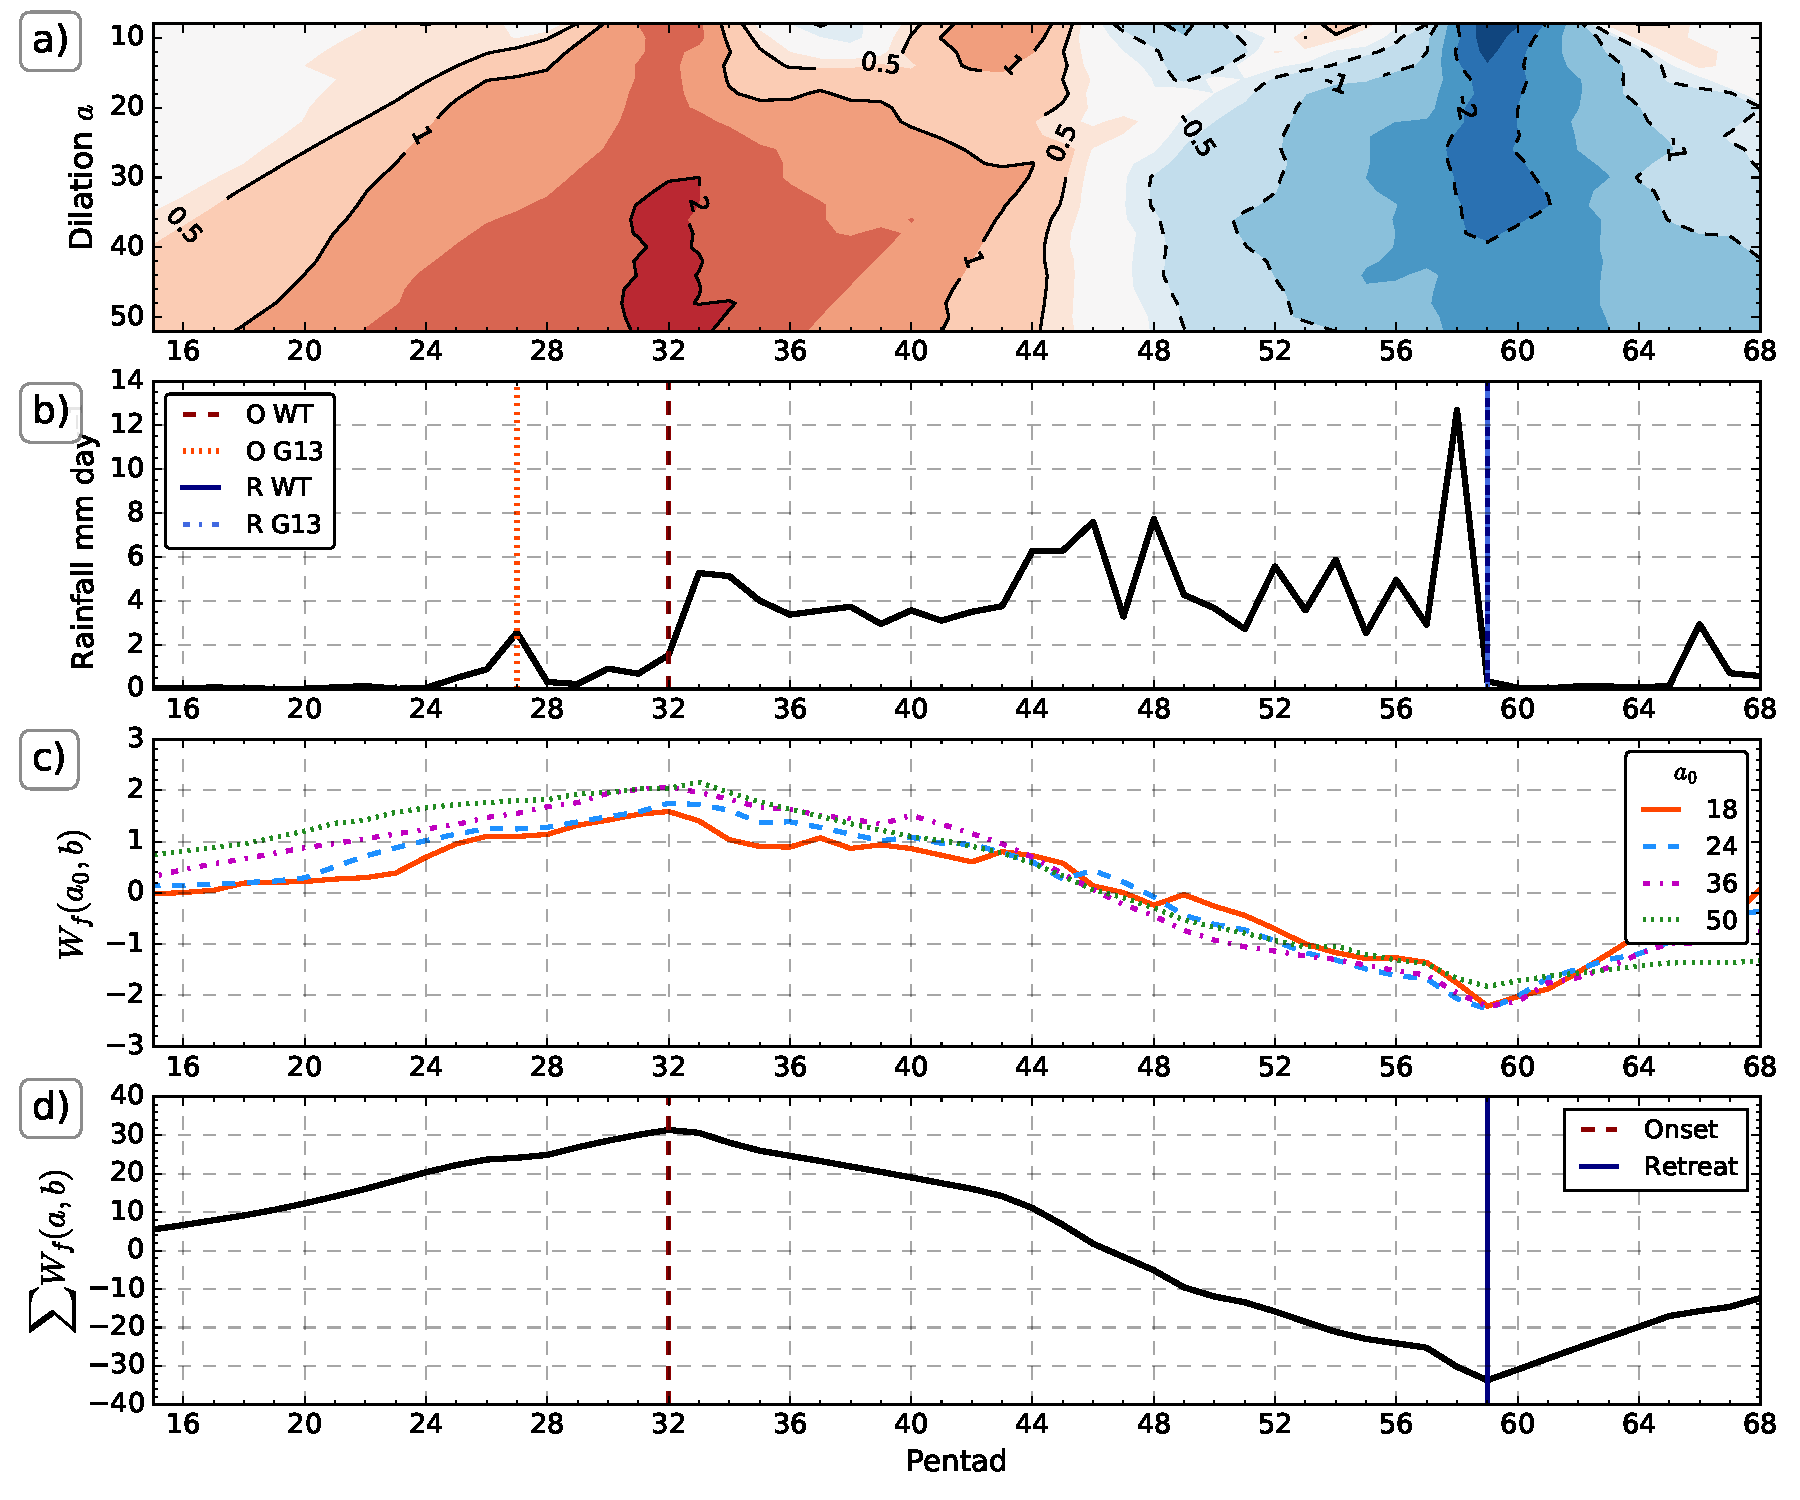
\includegraphics[width=\linewidth]{figures/wav_fig3.pdf}
\caption[Example determination of onset and retreat in TRMM]{ Example determination of monsoon onset and retreat dates for the North American Monsoon [20-27$^\circ$N,109-103$^\circ$W] in the TRMM dataset for 2009.
(a) WT coefficient matrix (mm d$^{-1}$) as a function of time and dilation coefficient $a$. The shading is from -3 to 3 mm d$^{-1}$  with an interval of 0.5 mm d$^{-1}$.
(b) Observed precipitation, the onset and retreat dates as determined by the WT method (dashed) and the threshold method of \cite{geil2013} (solid) are shown. Note that the date of retreat is diagnosed to be the same between the two methods.
(c) The WT coefficients for different dilations. (d) The sum of the WT ($\sum W_f(a,b)$) (mm d$^{-1}$); the maximum and minimum are shown in red and blue, representing onset and retreat pentads, respectively.  }
\label{fig:wvt_3}
\end{figure}

In other words, we seek to find monsoon onset and retreat using the maximum and minimum the wavelet power spectrum over a range of temporal scales.
Several sensitivity tests were performed with different dilation coefficients ($a$) in the different observational datasets, models and regions and a set or vector of dilation scales was found to be optimal. 
The set of dilation coefficients $\vec{a} = (28,30,\cdots, 54)$ was found to be robust, i.e., was able to capture the onset and retreat dates in all the datasets.

 Monsoon onset is defined as the maximum sum of wavelet coefficients, capturing positive gradients within the scales of 14 to 27 pentads (half of the elements of vector $a$ defined above). Monsoon Retreat has a similar definition, capturing the greatest negative gradient of precipitation over the same pentad scales.

For example, Figure \ref{fig:wvt_3} illustrates the method in the North American Monsoon in the TRMM dataset for 2009. Figure \ref{fig:wvt_3}a shows the WT coefficient matrix, showing the changes in precipitation for dilations ranging from 10 to 50. A clear signal of positive coefficients is observed between pentads 28 to 34  and a similar negative signal observed in pentads 56 to 60. Figure \ref{fig:wvt_3}b shows the time-series of the observed precipitation, which suggests that monsoon onset occurs sometime between pentads 28 and 34. Observed rainfall rapidly decreases after pentad 59 suggesting that monsoon retreat can be diagnosed around this pentad.

\begin{figure}
 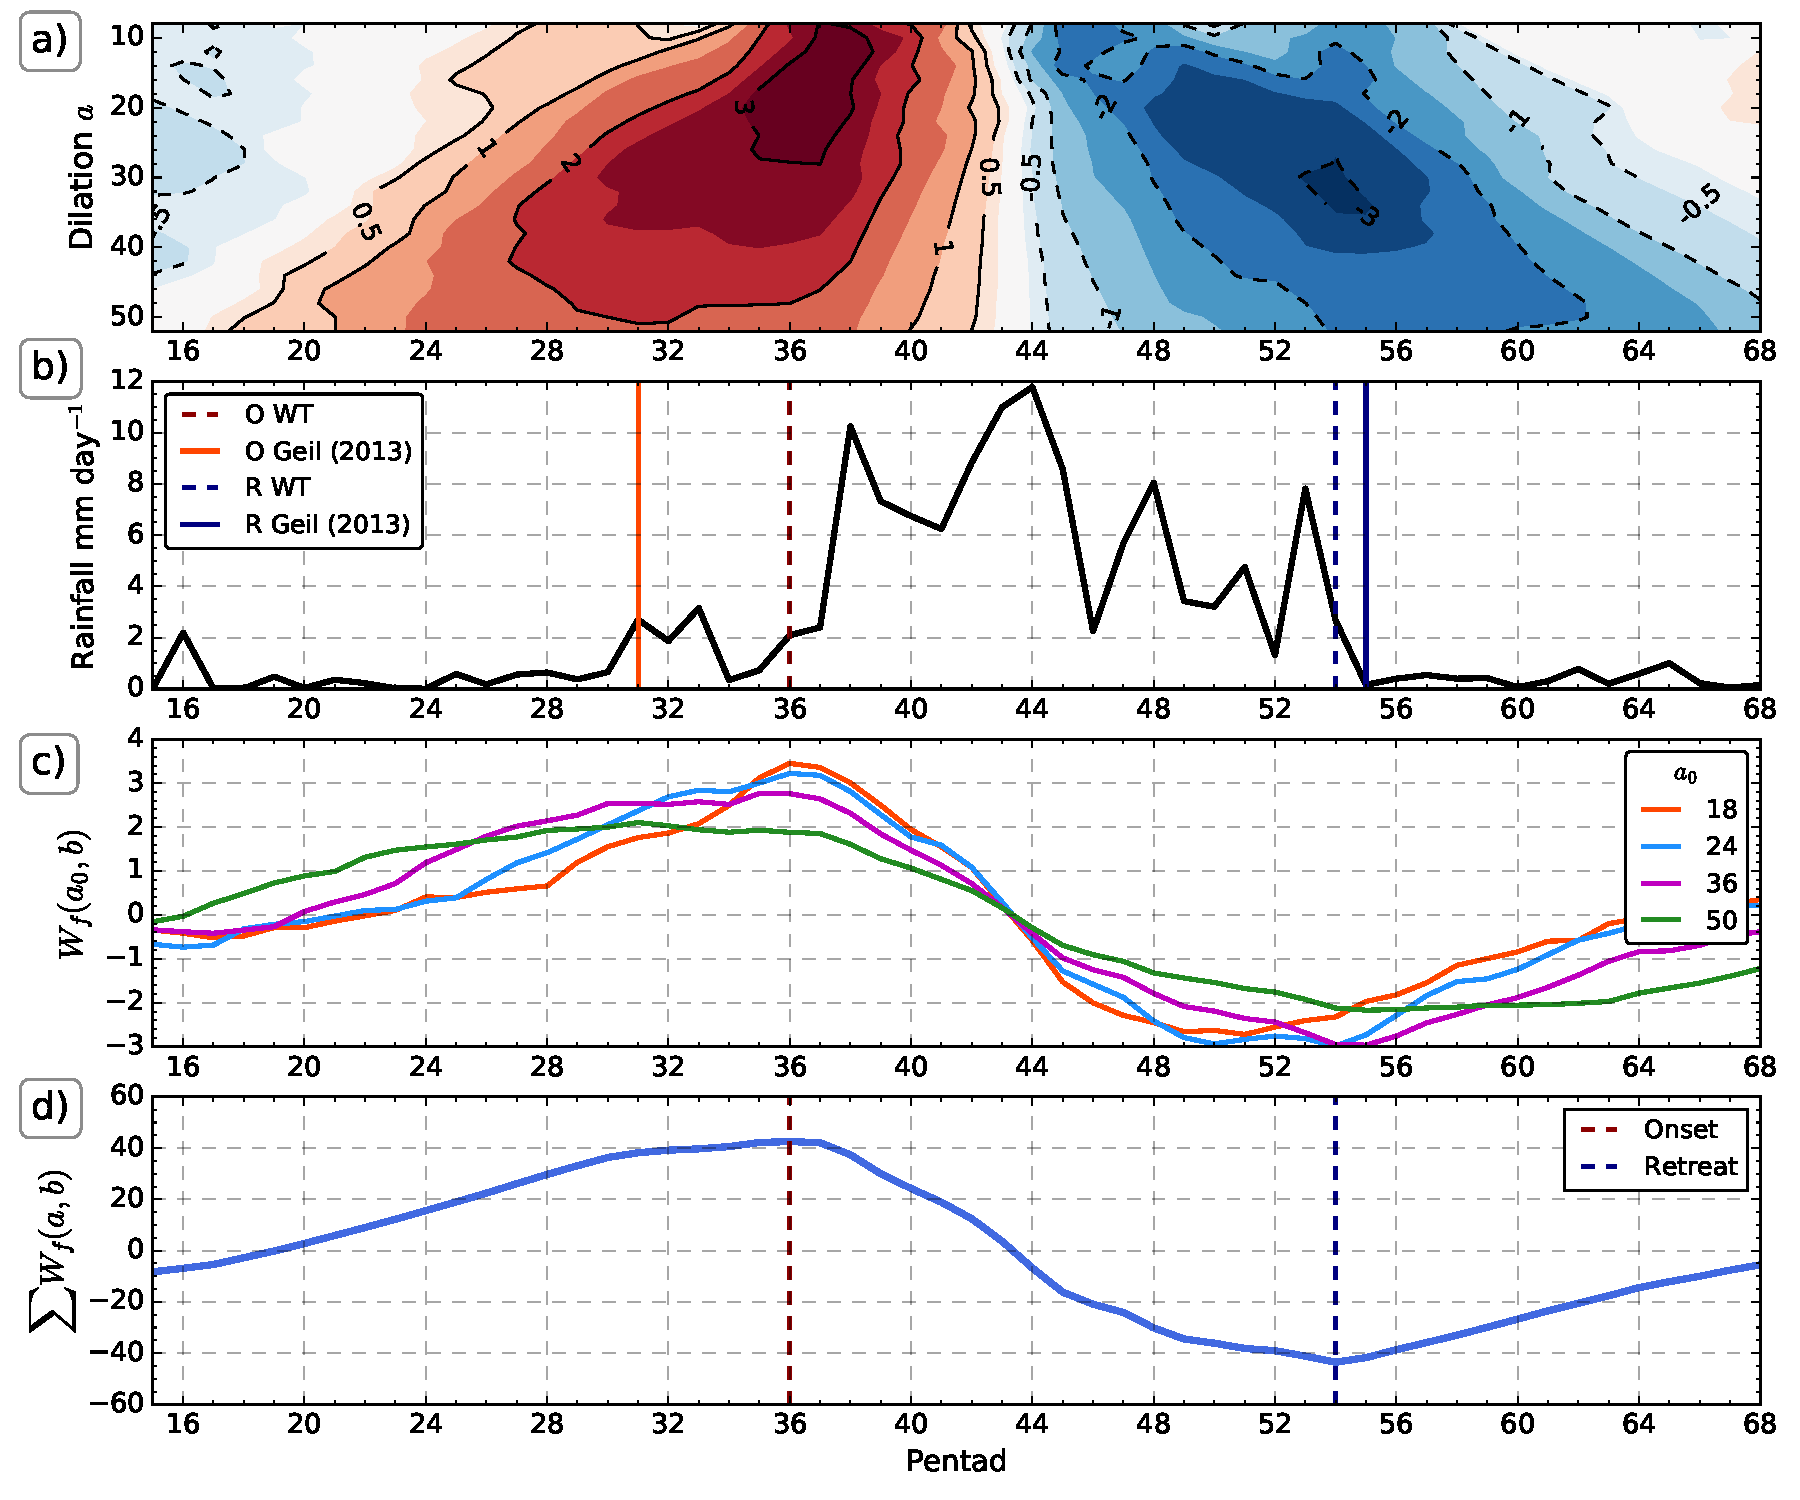
\includegraphics[width=\linewidth]{figures/nam_n216.pdf}
\caption[Example determination of onset and retreat in HadGEM3 N216]{ As in Figure \ref{fig:wvt_3}, but for a year (1875) in the HadGEMGC3.1 N216 pre-industrial control simulation.  }
\label{fig:s1_n216}
\end{figure}

 Figure \ref{fig:wvt_3}c shows the WT coefficients as a function of pentad for several dilations ($a_0$). The coefficients for all scales seem to follow a very similar behaviour, increasing during spring to reach a maximum around pentad 32 and thereafter decreasing to a minimum around pentad 59. When the sum of the wavelet transform coefficients across the dilations is computed (Figure \ref{fig:wvt_3}d) this behaviour becomes much clearer. The maximum and minimum are found at pentads 32 and 59, respectively and these pentads define the onset and retreat times. For comparison, the results from the method of \cite{geil2013} are shown in Figure \ref{fig:wvt_3}b, indicating that this method may have found an earlier onset. 
 
 As a proof of concept, Figure \ref{fig:s1_n216} shows a similar example using precipitation area-averaged in the same region but using model data from the piControl simulation of HadGEM3 GC3.1 N216. 
 The results show that the WT method can capture the onset and retreat dates with relatively high skill and that these dates are different from the dates computed using the method of \citetalias{geil2013}, with the threshold method suggesting an earlier onset and a later retreat. 

\subsection{Extension for Application to the MSD signal}




The wavelet method can be extended to characterise the shorter scale variations of precipitation of the MSD in Central America and the Caribbean. First, the monsoon onset and retreat dates are determined in the time-series from the area-averaged precipitation in the MSD region via the approach described in the previous section. 
Once the onset and retreat dates are established, an additional wavelet analysis determines the dates in which the MSD starts and ends.
The onset and end of the drier period of the MSD can be found by computing the wavelet transform again but using smaller dilations and over a limited temporal range. In particular, the WT is only calculated in the 20 pentads before and after the dates defining monsoon retreat and onset, respectively. The MSD Onset (MSDO) and MSD End (MSDE) are defined as the minimum and maximum, respectively, of the sum of the wavelet transforms (equations \ref{eq:mo} and \ref{eq:mr}) using dilation coefficients $\vec{a^*} = (10,12,\cdots, 24)$.
The diagnosis of the onset and end of the MSD is algo robust to using other dilation coefficients of similar magnitude.

Figure \ref{fig:5} illustrates the use of the WT method to determine the dates of MSDO and MSDE for the precipitation of 2017 in ERA-5.
Figure \ref{fig:5}a depicts the wavelet covariant transform matrix, showing the $W_f$ coefficients for each dilation $a$ at each pentad $b$. The onset of rainfall is diagnosed around the time-steps of highest positive $W_f$ coefficients -- around pentads 24 to 32 for almost all dilations. These positive coefficients are followed by a period of negative values from pentad 32 to pentad 40, which represent the decrease in precipitation, or relative drought, in the midsummer. The MSD is followed by another period of positive coefficients from pentad 44 to pentad 52, illustrating the so-called second peak of precipitation and, finally, a period of negative coefficients associated with monsoon retreat.

\begin{figure}[b!]
\centering
 %\noindent
 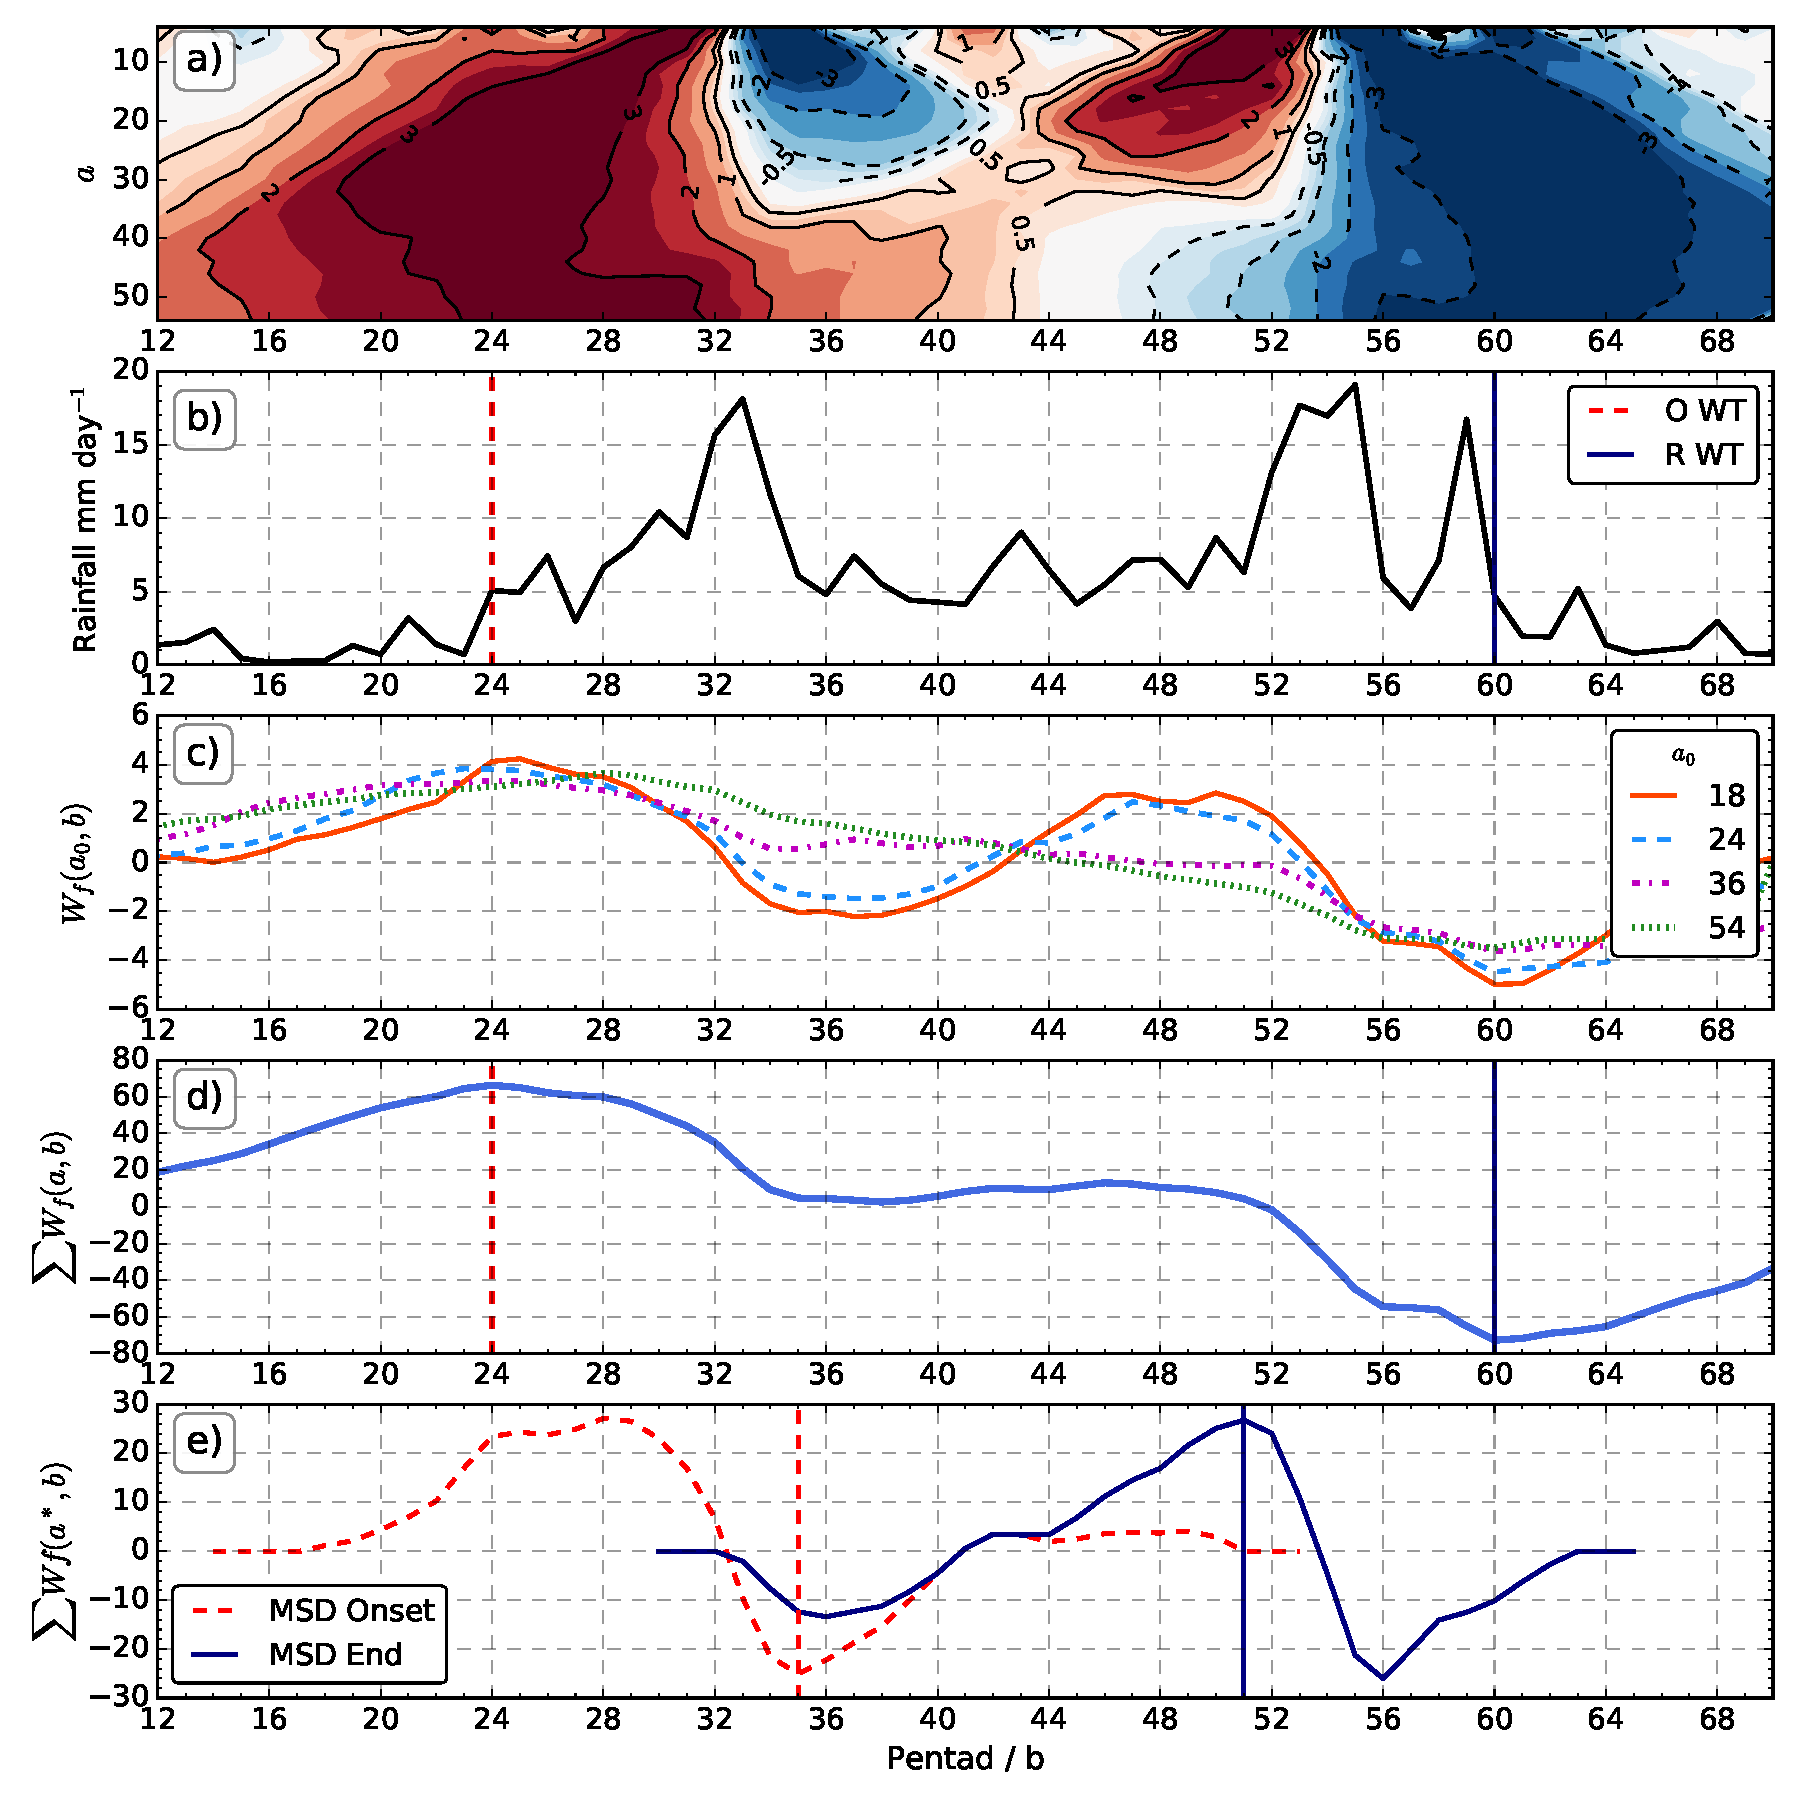
\includegraphics[width=\linewidth]{figures/wav_fig4.pdf}
\caption[Wavelet transform characterisation of Midsummer drought]{ Example characterisation of the MSD [11-19$^\circ$N,95-85$^\circ$W] using ERA-5 data for 2017. (a) Wavelet transform spectra, (b) observed precipitation with the onset and retreat pentads shown in red and blue, respectively. (c) Wavelet transform coefficients for four different dilations (mm d$^{-1}$). (d) The sum of the wavelet transform coefficients (mm d$^{-1}$) for $a={28,..,51}$. (e) The sum of $W_f(a,b)$ (mm d$^{-1}$) for dilation coefficients $a={12,..,24}$ showing the start (MSD Onset) and end (MSD End) of the midsummer drought. }
\label{fig:5}
\end{figure}

The coefficients of the wavelet transform ($W_f(a_0,b)$) for selected dilations $a_0$  (Figure \ref{fig:5}c) show that the smaller dilations are more sensitive to smaller scale variations in the time series and longer dilations better highlight the long-term change of the time series. For example $a_0=18$ shows signs of a MSD by showing two local maxima and two local minima, whereas $a_0=54$ only shows a local maximum and a local minimum associated with onset and retreat.

The maximum and minimum of the sum over all dilations (Figure \ref{fig:5}) depict the rainfall onset and retreat dates, respectively. The second wavelet transform $W_f(a^*,b)$ is computed over smaller dilation coefficients ($a^*$) near the onset and retreat dates as described above to highlight the MSDO and the MSDE.
Figure \ref{fig:5}e shows the sum of the wavelet transform coefficients  $W_f(a^*,b)$ and the pentad of the MSDO, 34, and MSDE, 49, corresponding to the minimum and maximum of the sum of these wavelet transform coefficients, respectively.

The strength of the MSD can be measured through the maximum and minimum sum of the coefficients $\sum W_f(a^*,b)$ used to define the start and end dates of the MSD.
For example, in Figure \ref{fig:5}e the minimum of the $\sum W_f(a^*,b)$ was -20\ mm\,d$^{-1}$ found at pentad 35 and an opposite local maximum of +20\ mm\,d$^{-1}$ at pentad 49. These two values, hereafter $coef1$ and $coef2$, provide a quantitative measure of the strength of the MSD for this year in this dataset and will be used to measure the spatial and temporal variability of the magnitude of the MSD in the different datasets.

\subsection{Comparative Methodologies}


For validation purposes, the wavelet transform method is compared with existing methods which determine onset and retreat in the North American and Indian monsoons. 
The threshold methods of \cite{geil2013} (hereafter G13) and \cite{arias2012} (hereafter A12) are compared to the results of the wavelet transform in the North American Monsoon.
\citetalias{geil2013} used a threshold of 1.3 mm day$^{-1}$ for at least 3 days for onset and 7 days for retreat for daily TRMM observations. This study, in contrast, analyses most of the data on the pentad-scale, so we adapt this method for TRMM to the same threshold value, but the onset pentad is the first pentad above the threshold whereas for retreat, we require rainfall to be below the threshold for two consecutive pentads.
 The method of \citetalias{arias2012} defines onset with two conditions. The first condition to find the onset pentad is that six out of the eight subsequent pentads must have rain-rates above the annual-mean climatological rainfall. The second condition is that at least six out of the eight previous pentads must be below the annual-mean climatological rainfall.
The opposite definition is used to determine the pentad of monsoon retreat. 

In relation for the Indian Monsoon region, a commonly used metric is the hydrological onset and withdrawal index (HOWI) which is based on moisture transport over the Arabian Sea \citep{fasullo2003,Sahana_2015,chevuturi2019}.
To compute the HOWI index, first, the vertically integrated moisture transport ($\chi$) is computed from daily ERA-5 data in the Arabian sea, as described by \cite{fasullo2003}, i.e.:

\begin{equation}
\chi=\frac{1}{g}\int_{p_0}^0 q \mathbf{V} dp,
\end{equation}
 \noindent where $g$ is the gravitational acceleration, $p$ are the pressure levels, $q$ is the specific humidity and $\mathbf{V}$ is the wind vector. The VIMT is then normalized using the transformation:

 \begin{equation}
 HOWI = 2 \bigg(\frac{\chi - min(\bar{\chi})}{max(\bar{\chi})-min(\bar{\chi})} \bigg)
 \end{equation}

 \noindent where $\chi$ is the unnormalized time-series, $\bar{\chi}$ is the mean seasonal cycle of the unnormalized index and HOWI is the normalized index. The onset date is defined as the first day of each year where the HOWI index is greater than zero and the retreat date is the first day after the onset date that the HOWI index is negative \citep{fasullo2003,Sahana_2015}.
 The necessary daily data of moisture and wind speed on sufficient vertical levels to compute the HOWI index in the MOHC submissions to CMIP6 was not available, so the HOWI index can only be computed using ERA5 and will be compared to the WT method used on the observational gridded datasets.

\section{Results}

\begin{table}[b!]
% table caption is above the table
\caption{Mean (standard deviation) pentads of monsoon onset (O) and retreat (R) in the North American Monsoon [110$^\circ$-103$^\circ$W, 20$^\circ$-27$^\circ$N] for observational datasets, reanalysis and model output with the wavelet transform method WT, G13's and A14's method. Pentad 34 corresponds to the period between June 17-22 and pentad 54 to the period Sep 27 - Oct 1. The results from the WT method in the model experiments which are statistically different to both the CMAP and CHIRPS results at the 95\% confidence level, according to a Welch's t-test, are shown in bold. }
\label{tab:3}       % Give a unique label
% For LaTeX tables use
\begin{tabular}{p{2.2cm}p{1.765cm}p{1.765cm}p{1.765cm}p{1.765cm}p{1.7655cm}p{1.7655cm}}
\hline\noalign{\smallskip} \small
Dataset / Experiment & WT O 	& WT R 	& G13 O & G13 R & A12 O & A12 R \\ \hline
TRMM & 33.3 [$\pm$1.8] & 55.8 [$\pm$1.9] & 33.0 [$\pm$1.7] & 56.6 [$\pm$1.4] & 30.4 [$\pm$1.7] & 53.8 [$\pm$2.0]  \\
CMAP & 33.2 [$\pm$1.6] & 55.0 [$\pm$2.1] & 36.0 [$\pm$3.3] & 55.7 [$\pm$1.8] & 31.7 [$\pm$3.0] & 54.5 [$\pm$3.3]   \\
CHIRPS & 32.5 [$\pm$1.5] & 54.7 [$\pm$1.9] & 33.6 [$\pm$1.7]& 56.1 [$\pm$1.4] & 30.1 [$\pm$1.7] & 53.6 [$\pm$2.5]   \\
ERA-5 & 33.5 [$\pm$1.8] & 55.5 [$\pm$2.0] & 33.6 [$\pm$1.8]& 56.4 [$\pm$1.4] & 30.9 [$\pm$1.7] & 53.3 [$\pm$2.3]   \\
GC3 N216-pi  & 33.7 [$\pm$2.0] & 55.1 [$\pm$1.8]& 32.6 [$\pm$2.5] & 55.9 [$\pm$2.3] & 32.4 [$\pm$2.5] &53.8 [$\pm$3.8]  \\
GC3 N96-pi & 33.7 [$\pm$2.2] & 55.0 [$\pm$2.1] & 32.7 [$\pm$2.9] & 56.3 [$\pm$2.0] & 31.9 [$\pm$2.6] & 54.1 [$\pm$4.1]  \\
GC3-hist & 33.8 [$\pm$2.3] & 55.1 [$\pm$2.1]& 33.3 [$\pm$2.9] & 56.0 [$\pm$2.2] & 31.9 [$\pm$2.6] & 53.7 [$\pm$4.0]  \\
UKESM-pi & \bf{34.5} [$\pm$2.1] & 54.8 [$\pm$2.1] & 34.1 [$\pm$2.9] & 56.1 [$\pm$1.9] & 33 [$\pm$2.6] & 53.9 [$\pm$4]   \\
UKESM-hist & \bf{34.3} [$\pm$2.2] & 54.3 [$\pm$2.2]& 34.4 [$\pm$3.2] & 55.6 [$\pm$2.1] & 33.1 [$\pm$3.0] & 53.2 [$\pm$4.2] \\
%\noalign{\smallskip}\hline\noalign{\smallskip}
%number & number & number \\
%number & number & number \\
%\noalign{\smallskip}\hline
\end{tabular}
\end{table}


The monsoon onset and retreat dates were determined for each year in each observational and model dataset for the Indian, North American and MSD regions using the methods described in the previous section. The calculations were performed for area-averaged precipitation time-series representative of the core regions defining these monsoons. Calculations were also made at grid-box scales to illustrate the spatial distribution of the onset and retreat dates. 


\subsection{The North American Monsoon}






Table \ref{tab:3} shows the mean onset and retreat dates estimated using the \citetalias{geil2013}, \citetalias{arias2012} and WT methods for precipitation time-series averaged over the North American monsoon.
The table reports the results for three observational datasets, ERA-5 reanalysis and five climate model experiments.
The observations  agree that the onset date is found at pentad 33 (around June 15), according to the WT and the method by \citetalias{geil2013}.
However, the method of \citetalias{geil2013} reports a mean retreat date that is one pentad later than the WT method, i.e., around October 7th for G13 method and October 2nd for the WT.
The method by \citetalias{arias2012} disagrees with \citetalias{geil2013} and the WT methods for both onset and retreat mean pentads, in both cases finding an earlier onset (pentad 30) and retreat (pentad 54) for all the observational datasets. 

\begin{figure}[t!]
\centering
 %\noindent
 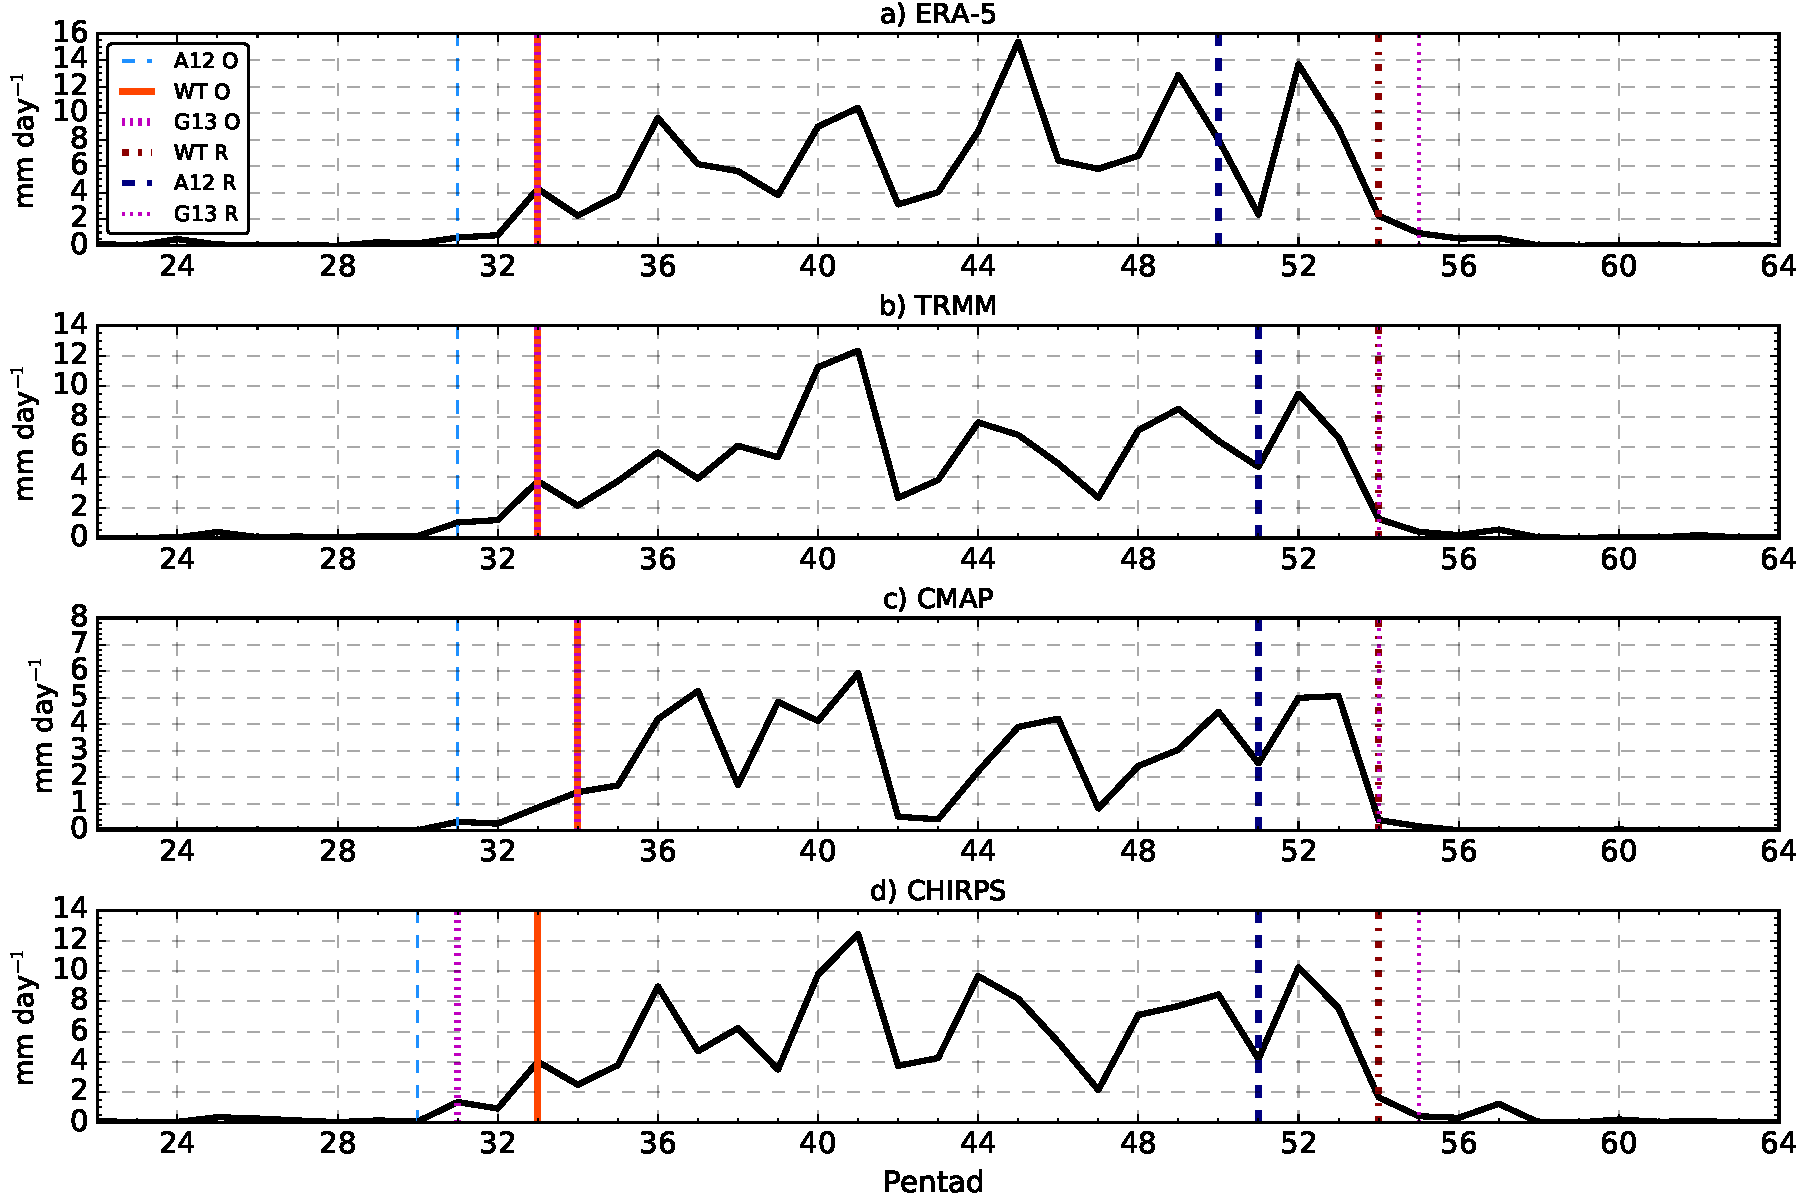
\includegraphics[width=\linewidth]{figures/wav_fig5.pdf}
\caption[Comparison of methods in 2010 in the North American Monsoon]{  Pentad-mean precipitation for the North American Monsoon in 2010 in four precipitation datasets showing the onset and retreat pentads as diagnosed by the WT, the A12 and G13 methods. The area used to average the precipitation is illustrated in in Figure \ref{fig:wav_fig6}b).} 
\label{fig:wav_compari}
\end{figure}


\begin{figure}[t!]
\centering
 %\noindent
 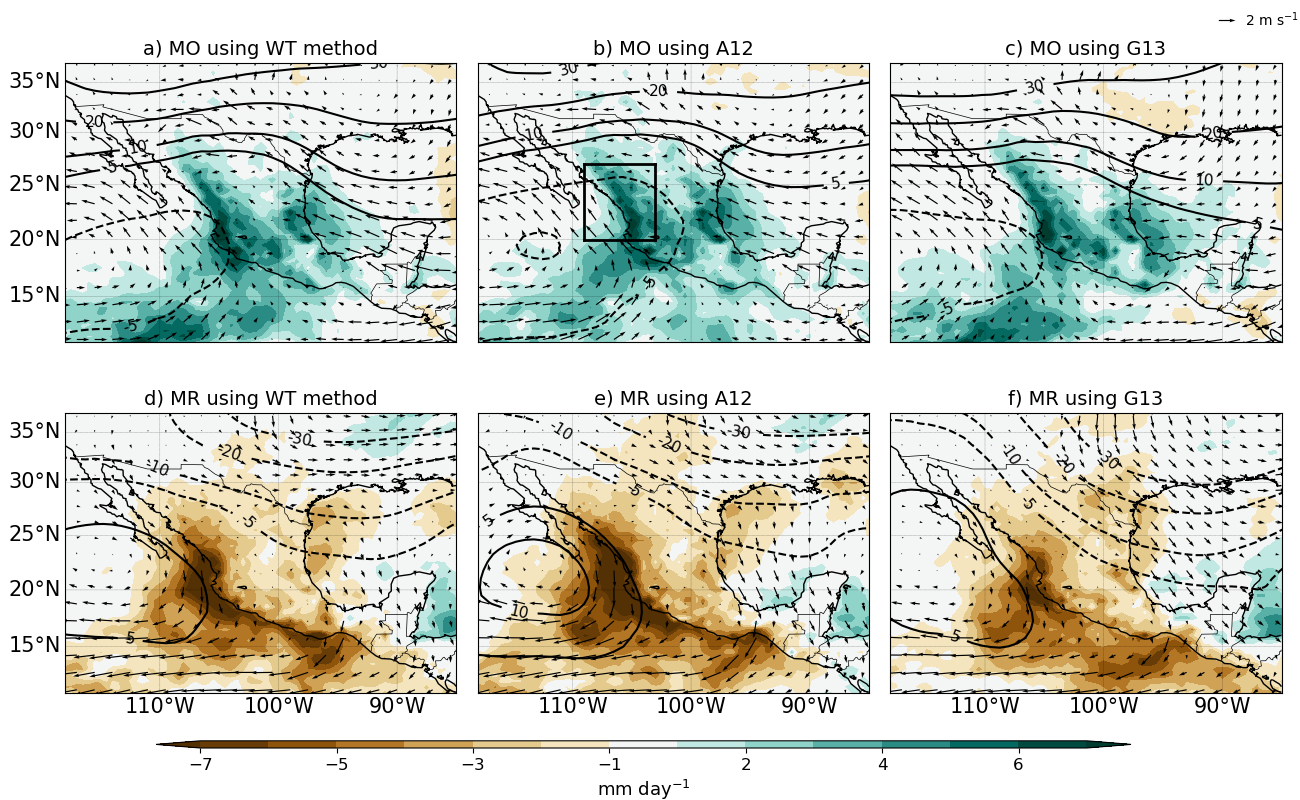
\includegraphics[width=\linewidth]{figures/wav_fig6.png}
\caption[Precipitation anomalies during North American monsoon onset]{  Precipitation (color contours), low level wind at 850-hPa and geopotential height (line contours) at 500 hPa anomalies for (a, b, c) the difference between the 10 days after monsoon onset and 10 days prior to onset (MO) using onset dates from (a) the WT (b) \cite{arias2012} and (c) \cite{geil2013}. (d, e, f) are as in (a, b, c) but for monsoon retreat. The data and dates are obtained from ERA-5, and the area for the average is shown in the box in b). }
\label{fig:wav_fig6}
\end{figure}

The climate models reasonably represent the mean onset and retreat dates, as only the onset dates from both experiments of UKESM1 are statistically different to the results of CMAP and CHIRPS. The similiarities in onset and retreat dates confirm that the seasonal cycle in the North American monsoon is very well represented by these models, as suggested by chapter \ref{ch:4-ams}. In the results of the simulations, \citetalias{arias2012} also produces an earlier onset and retreat dates when compared to the other two methods of about 1.5 pentads, but this difference is within the uncertainty range given by the interannual variability of the model data which is largest for  \citetalias{arias2012}.  

Figure \ref{fig:wav_compari} compares the estimated onset and retreat dates using the three methods for the 2010 North American Monsoon  using the three observational datasets and ERA5. \citetalias{arias2012} shows an earlier onset and retreat in all the datasets compared with the WT and \citetalias{geil2013} which agree in almost every dataset. The WT method is the only method that estimated the same retreat date for all the four datasets and the same onset date in three of the four datasets, with the CMAP datasets showing an onset date one pentad later than the others. % delayed by only one pentad. 

\begin{figure}[t!]
\centering
 %\noindent
 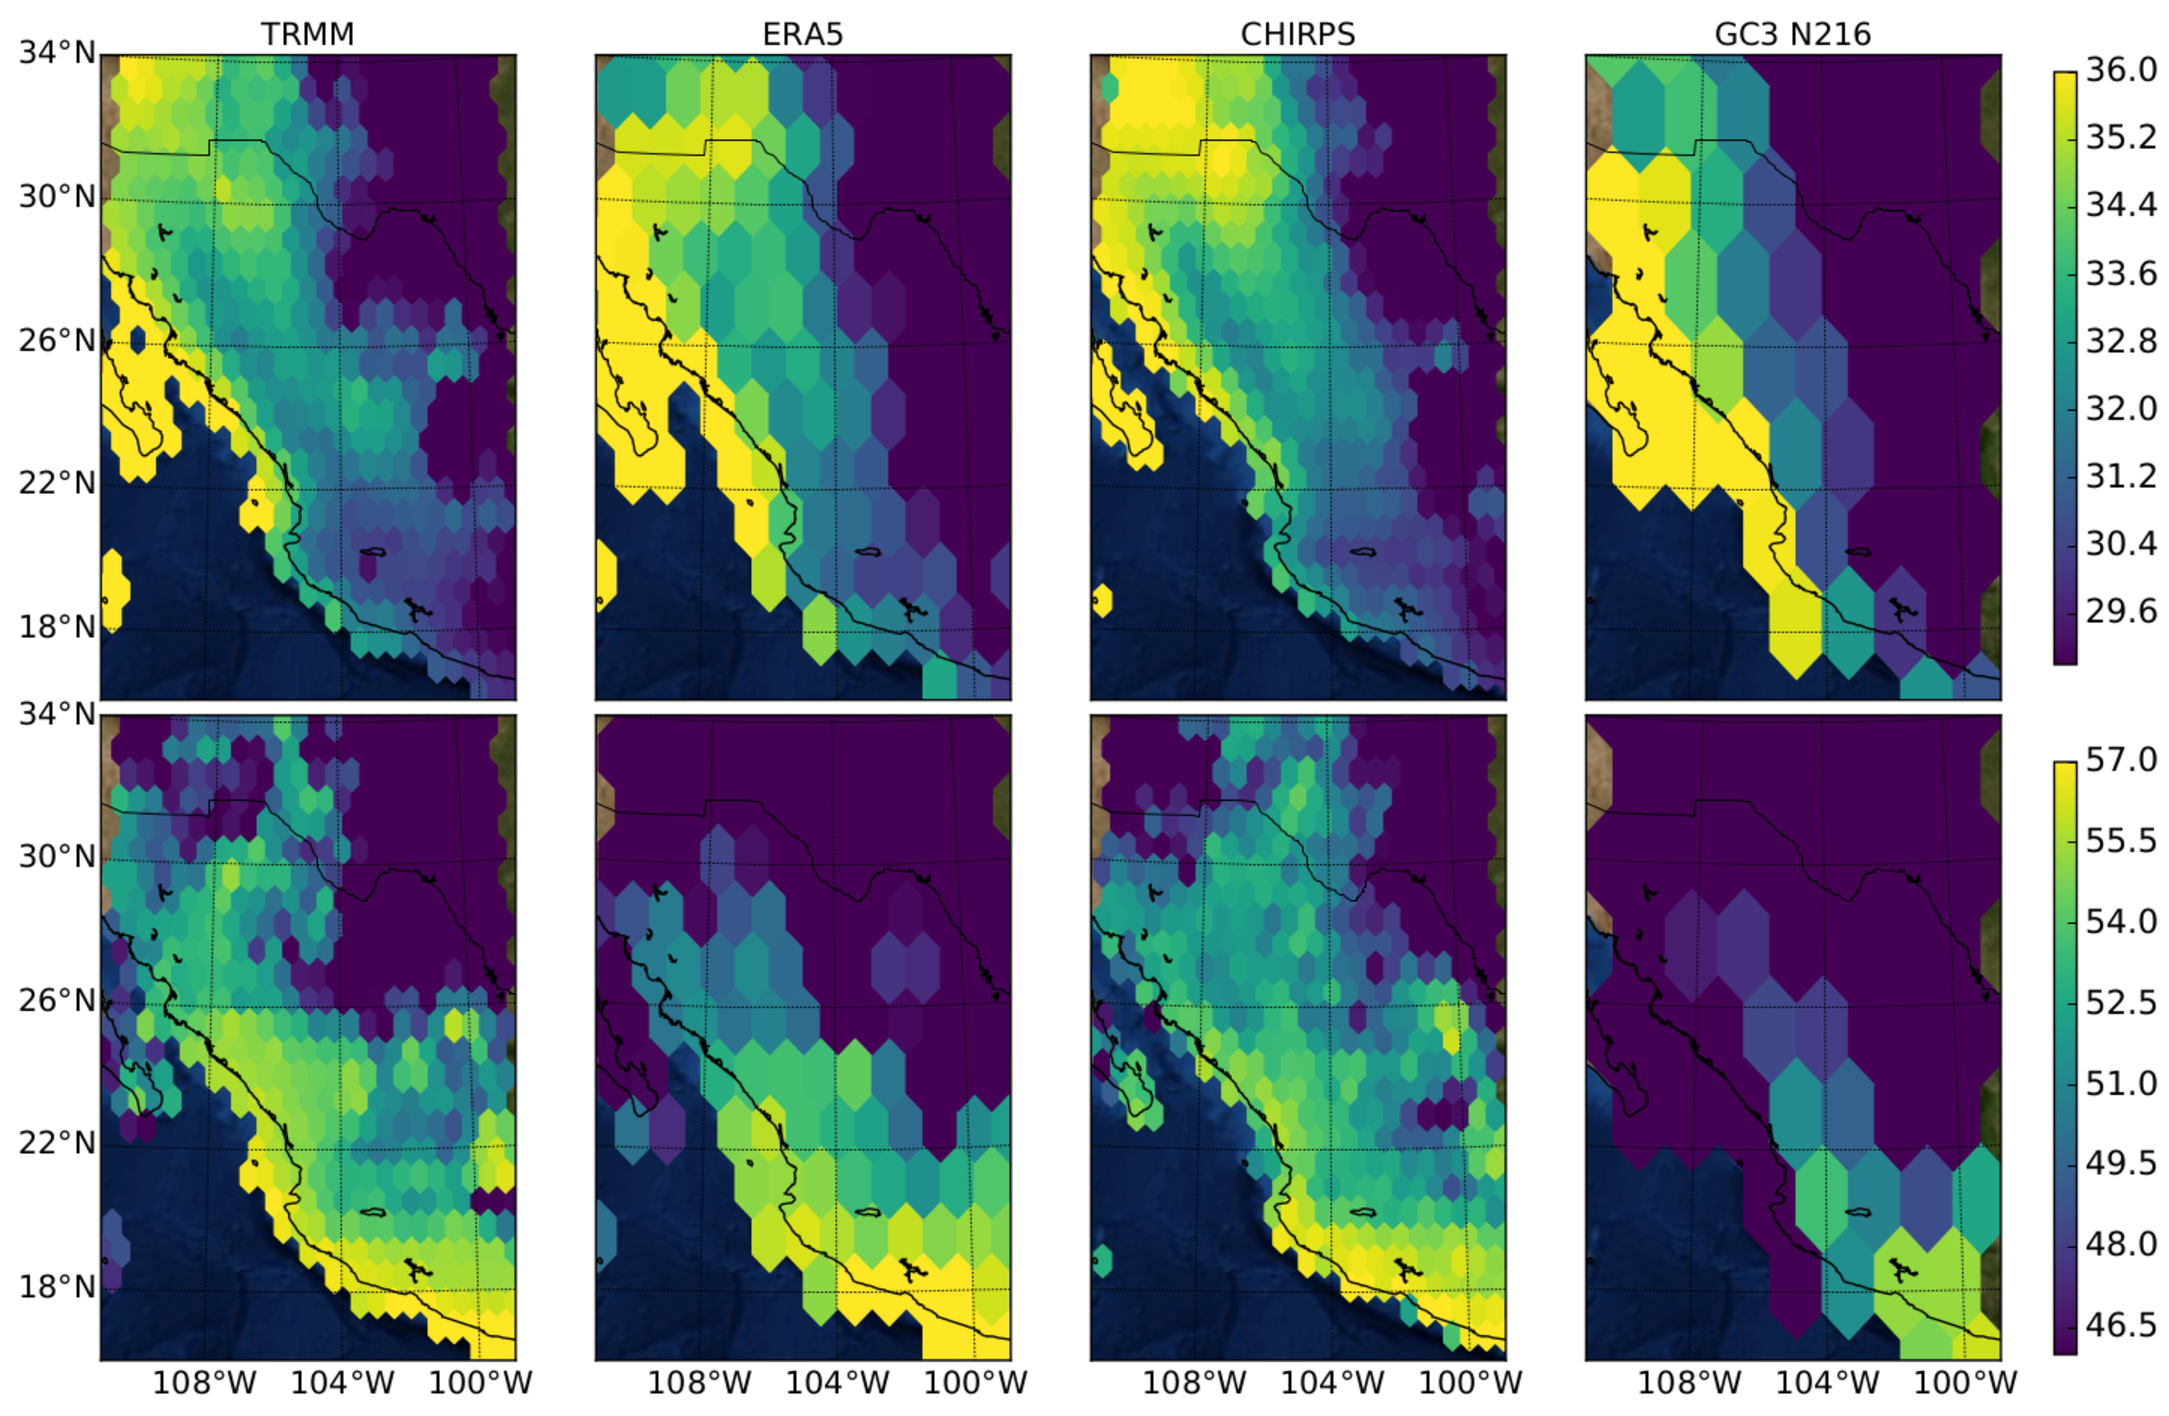
\includegraphics[width=\linewidth]{figures/map_nam_wav.pdf}
\caption[Onset and retreat spatial distribution in North American Monsoon]{ Rainfall onset (upper) and retreat (lower) mean pentads in the North American Monsoon for observations and a climate model output using the WT method.  }
\label{fig:nam_map}
\end{figure}

The meteorological changes associated with onset and retreat of the North American Monsoon  (Figure \ref{fig:wav_fig6}) are illustrated as the composite differences of the precipitation, wind and geopotential changes 10 days prior to and after onset and retreat. These changes to the circulation and precipitation are reasonably similar for all the three methods. The impact of monsoon onset in precipitation is diagnosed to be sligthly stronger by \citetalias{arias2012} compared to WT or \citetalias{geil2013}. 
The WT method shows a very similar pattern and magnitud of the circulation and precipitation anomalies of onset and retreat when compared to the other two methods. The method by \citetalias{geil2013} produces the weakest anomalies, particularly of precipitation whereas the method by \citetalias{arias2012} produces the strongest precipitation and geopotential anomalies, particularly at retreat.

Figure \ref{fig:nam_map} shows the spatial distribution of the mean onset and retreat dates in the North American Monsoon region for various datasets.
There is high agreement between TRMM, CHIRPS and ERA5 on the spatial pattern of mean onset and retreat dates.
Onset in western Mexico is around pentad 31 (around June 1st), whereas in Chihuahua and Sonora the rainy season begins shortly after pentad 35 (June 22).
The pattern in the medium-resolution simulation GC3 N216 piControl is consistent with observations, particularly during onset.  However, the spatial pattern of the mean retreat dates in the northern regions of the monsoon show an earlier than observed retreat, possibly associated with the dry bias in this region in these models (see chapter \ref{ch:4-ams}).

\subsection{The Indian Monsoon}
\begin{table}[b!]
% table caption is above the table
\caption{Mean (standard deviation) pentads of monsoon onset (MO) and retreat (MR) in the Indian Monsoon using the WT method on observed, reanalysed and modelled time-series as well as for the HOWI index. The region over which precipitation was area-averaged for the WT method was [75$^\circ$-83$^\circ$E, 18$^\circ$-24$^\circ$N]. The mean onset and retreat dates that are significantly different to the 99\% confidence level to the CMAP dataset are shown in bold.  }
\label{tab:3a}       % Give a unique label
% For LaTeX tables use
\begin{tabular}{p{4cm}p{3.5cm}p{3.5cm}}
\hline\centering{\smallskip}
Dataset & MO 	& MR 	\\ \hline
TRMM & 31.6 [$\pm$1.8] & 53.2 [$\pm$1.9]   \\
CMAP & 31.8 [$\pm$1.6] & 53.3 [$\pm$2.6]   \\
CHIRPS & 31.5 [$\pm$1.4] & 53.4 [$\pm$1.9]    \\
ERA-5 & 31.8 [$\pm$1.9] & 52.7 [$\pm$2.6]    \\
GC3 N216-pi  & {\bf34.4} [$\pm$1.3] & {\bf 50.5} [$\pm$1.9] \\
UKESM-pi & {\bf36.1} [$\pm$3.1] & {\bf 51.9} [$\pm$3.2]   \\
UKESM-hist & {\bf36.0} [$\pm$3.9] & {\bf51.8} [$\pm$3.3]   \\
GC3 N96-pi & {\bf35.5} [$\pm$1.8] & {\bf51.8} [$\pm$2.3]  \\
GC3-hist & {\bf35.7} [$\pm$2.1] & {\bf51.5} [$\pm$2.8]  \\
HOWI (ERA5) & {\bf29.5} [$\pm$2.3] & {\bf49.3} [$\pm$2.4]
%GC3.1 N216  & 33.4 [$\pm$3.1] & 56.1 [$\pm$2.5]  \\
%GC3 hist & 34.5 [$\pm$7.2] & 56.4 [$\pm$7.3]   \\
%UKESM hist & 35.2 [$\pm$2.3] & 55.1 [$\pm$8.8] \\
%\noalign{\smallskip}\hline\noalign{\smallskip}
%number & number & number \\
%number & number & number \\
%\noalign{\smallskip}\hline
\end{tabular}
\end{table}

Table \ref{tab:3a} compares the mean onset and retreat dates of the Indian Monsoon as computed from the HOWI index using ERA5 data, and the WT used for gridded precipitation datasets.
The onset and retreat dates from the HOWI index were converted from the daily to the pentad-scale to compare with the WT. The mean onset date for the HOWI index is May 27th between pentads 29 and 30, and retreat is between pentads 49 and 50, around September 3rd. The mean onset date found using the WT method for the four observational datasets was pentad 32, about two pentads later than the HOWI index. The mean retreat date for the WT method (pentad 53) was two pentads later than the HOWI results.

\begin{figure}[t!]
\centering
 %\noindent
 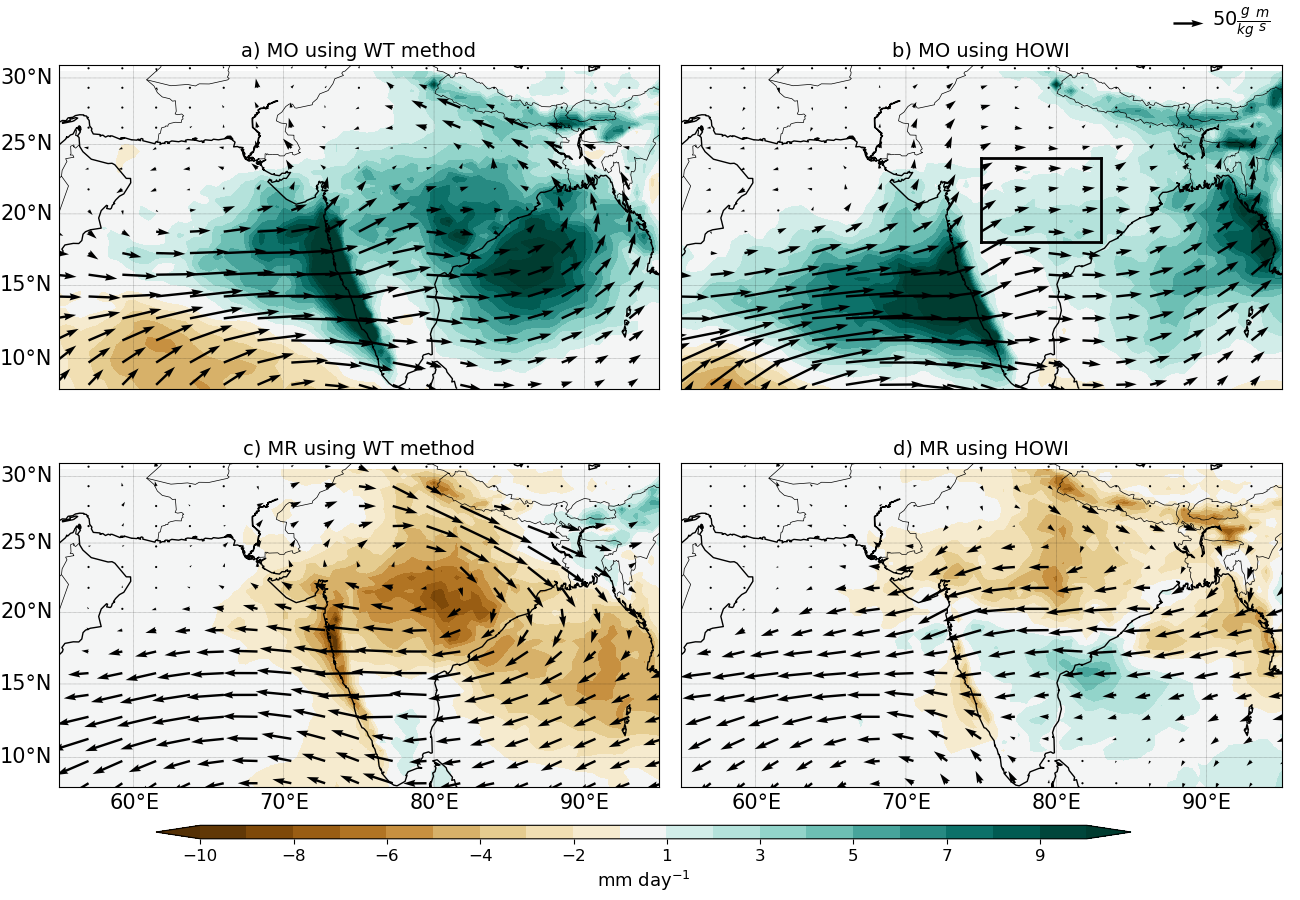
\includegraphics[width=0.95\linewidth]{figures/wav_fig8.png}
\caption[Precipitation anomalies during Indian monsoon onset]{  Precipitation anomalies (color contours) and the moisture flux vectors calculated from the product of specific humidity ($q$) and wind ($\vec{u}$) at 850 hPa. (a, b) shows the difference between the 10 days after monsoon onset and 10 days prior to MO using (a) the WT and (b) the dates estimated using the HOWI index. (c, d) are as defined in (a, b) but for MR. The dates are calculated from ERA5 data averaged over the box in panel b). }
\label{fig:wav_fig8}
\end{figure}

Overall, the models exhibited later than observed onset (+4 pentads) and earlier retreat  (-2 pentads) dates. The differences between the hydrological determination of onset and retreat dates, through HOWI, and the WT method on gridded precipitation datasets is statistically significant, according to a Welch's t-test comparing the HOWI and all the gridded datasets. These differences may be due to the different regions where each method is defined, i.e., HOWI is defined over the whole of the Arabian Sea where an earlier onset would be expected when compared to rainfall over mainland India, where the WT method was applied. 

\begin{figure}[t!]
\centering
 %\noindent
 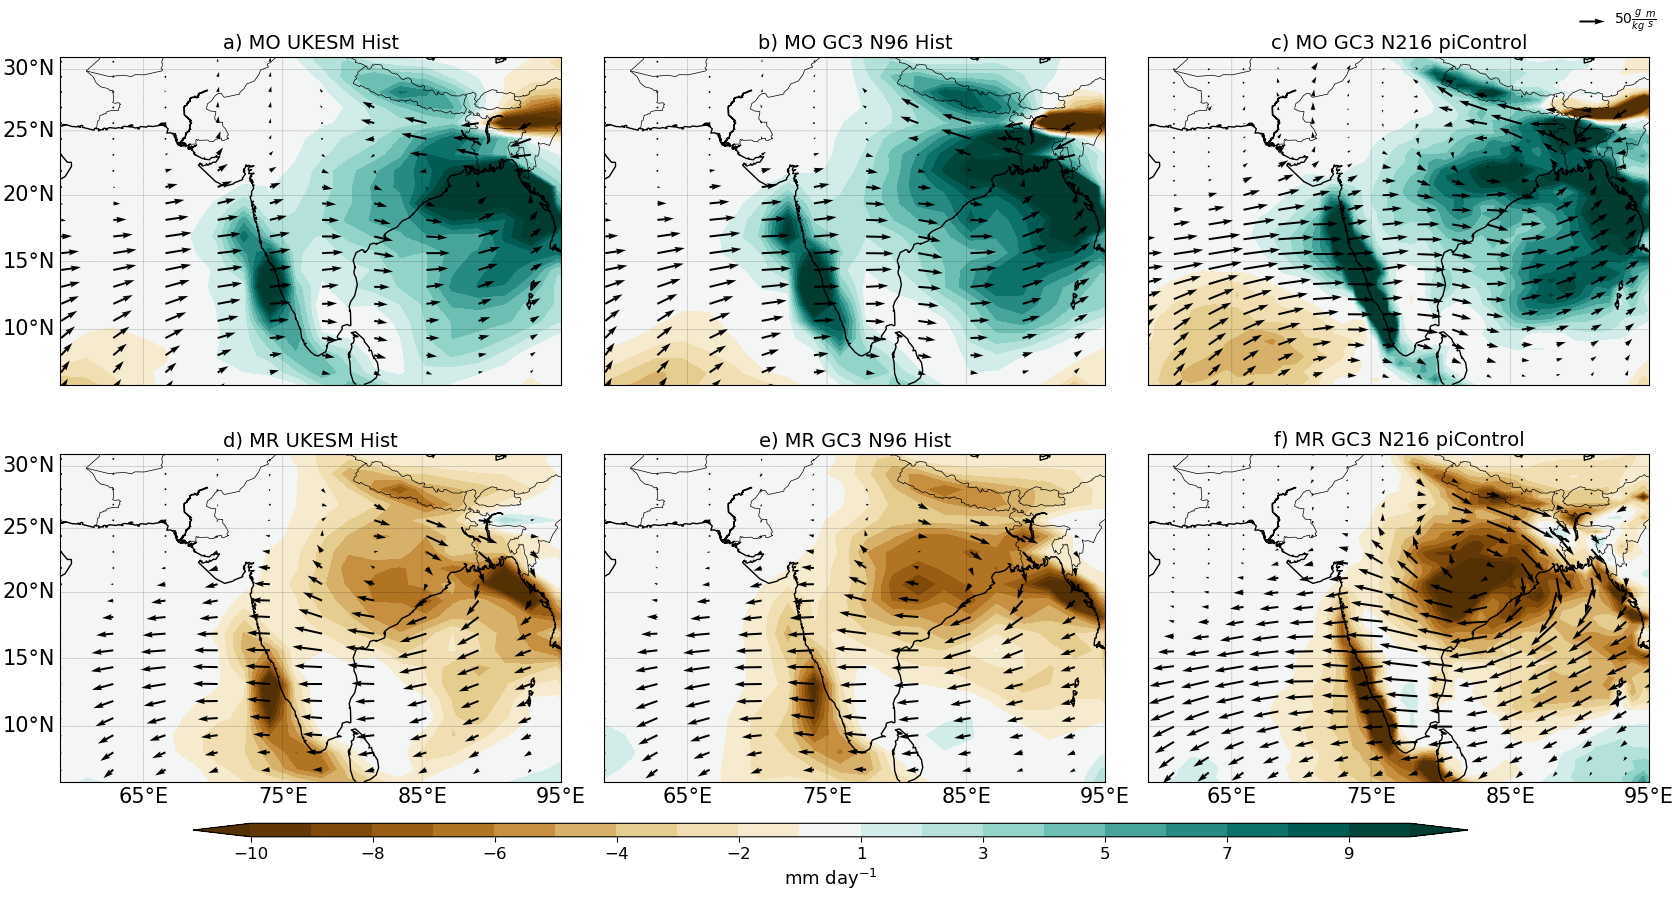
\includegraphics[width=\linewidth]{figures/ind_models.png}
\caption[Indian monsoon precipitation anomalies associated with onset]{ As in Figure \ref{fig:wav_fig8} but showing onset and retreat for three different climate model experiments: (a, d) UKESM1 historical, (b, e) HadGEM3 GC3.1 N96 historical, (c, f) HadGEM3 GC3.1 N216 piControl.   }
\label{fig:indmodels}
\end{figure}

Figure \ref{fig:wav_fig8} shows the differences between the WT (based on ERA5 precipitation) and HOWI methods in their characterisation of the meteorological changes associated with onset and retreat. 
The comparison of precipitation and moisture fluxes at 850 hPa anomalies 10 days prior to and following monsoon onset and retreat show that the HOWI index better captures the moisture transport in the Arabian Sea whereas the WT method best captures precipitation differences over mainland India. The HOWI index characterisation of the moisture flux in the Arabian Sea may be out-of-phase with precipitation over mainland India, and this lag could possibly explain some of the results of Table \ref{tab:3a}.


 The WT method is also able to capture onset and retreat dates and the associated anomalies within the climate model output. Figure \ref{fig:indmodels} shows the precipitation and moisture transport anomalies around the onset and retreat of the Indian monsoon in three different climate model experiments. While the models show significant biases in the timings of the monsoon, according to a Welch's t-test (Table \ref{tab:3a}), the patterns of rainfall and moisture transport anomalies to the observations around both onset and retreat agree well with reanalysis.

\begin{figure}
\centering
 %\noindent
 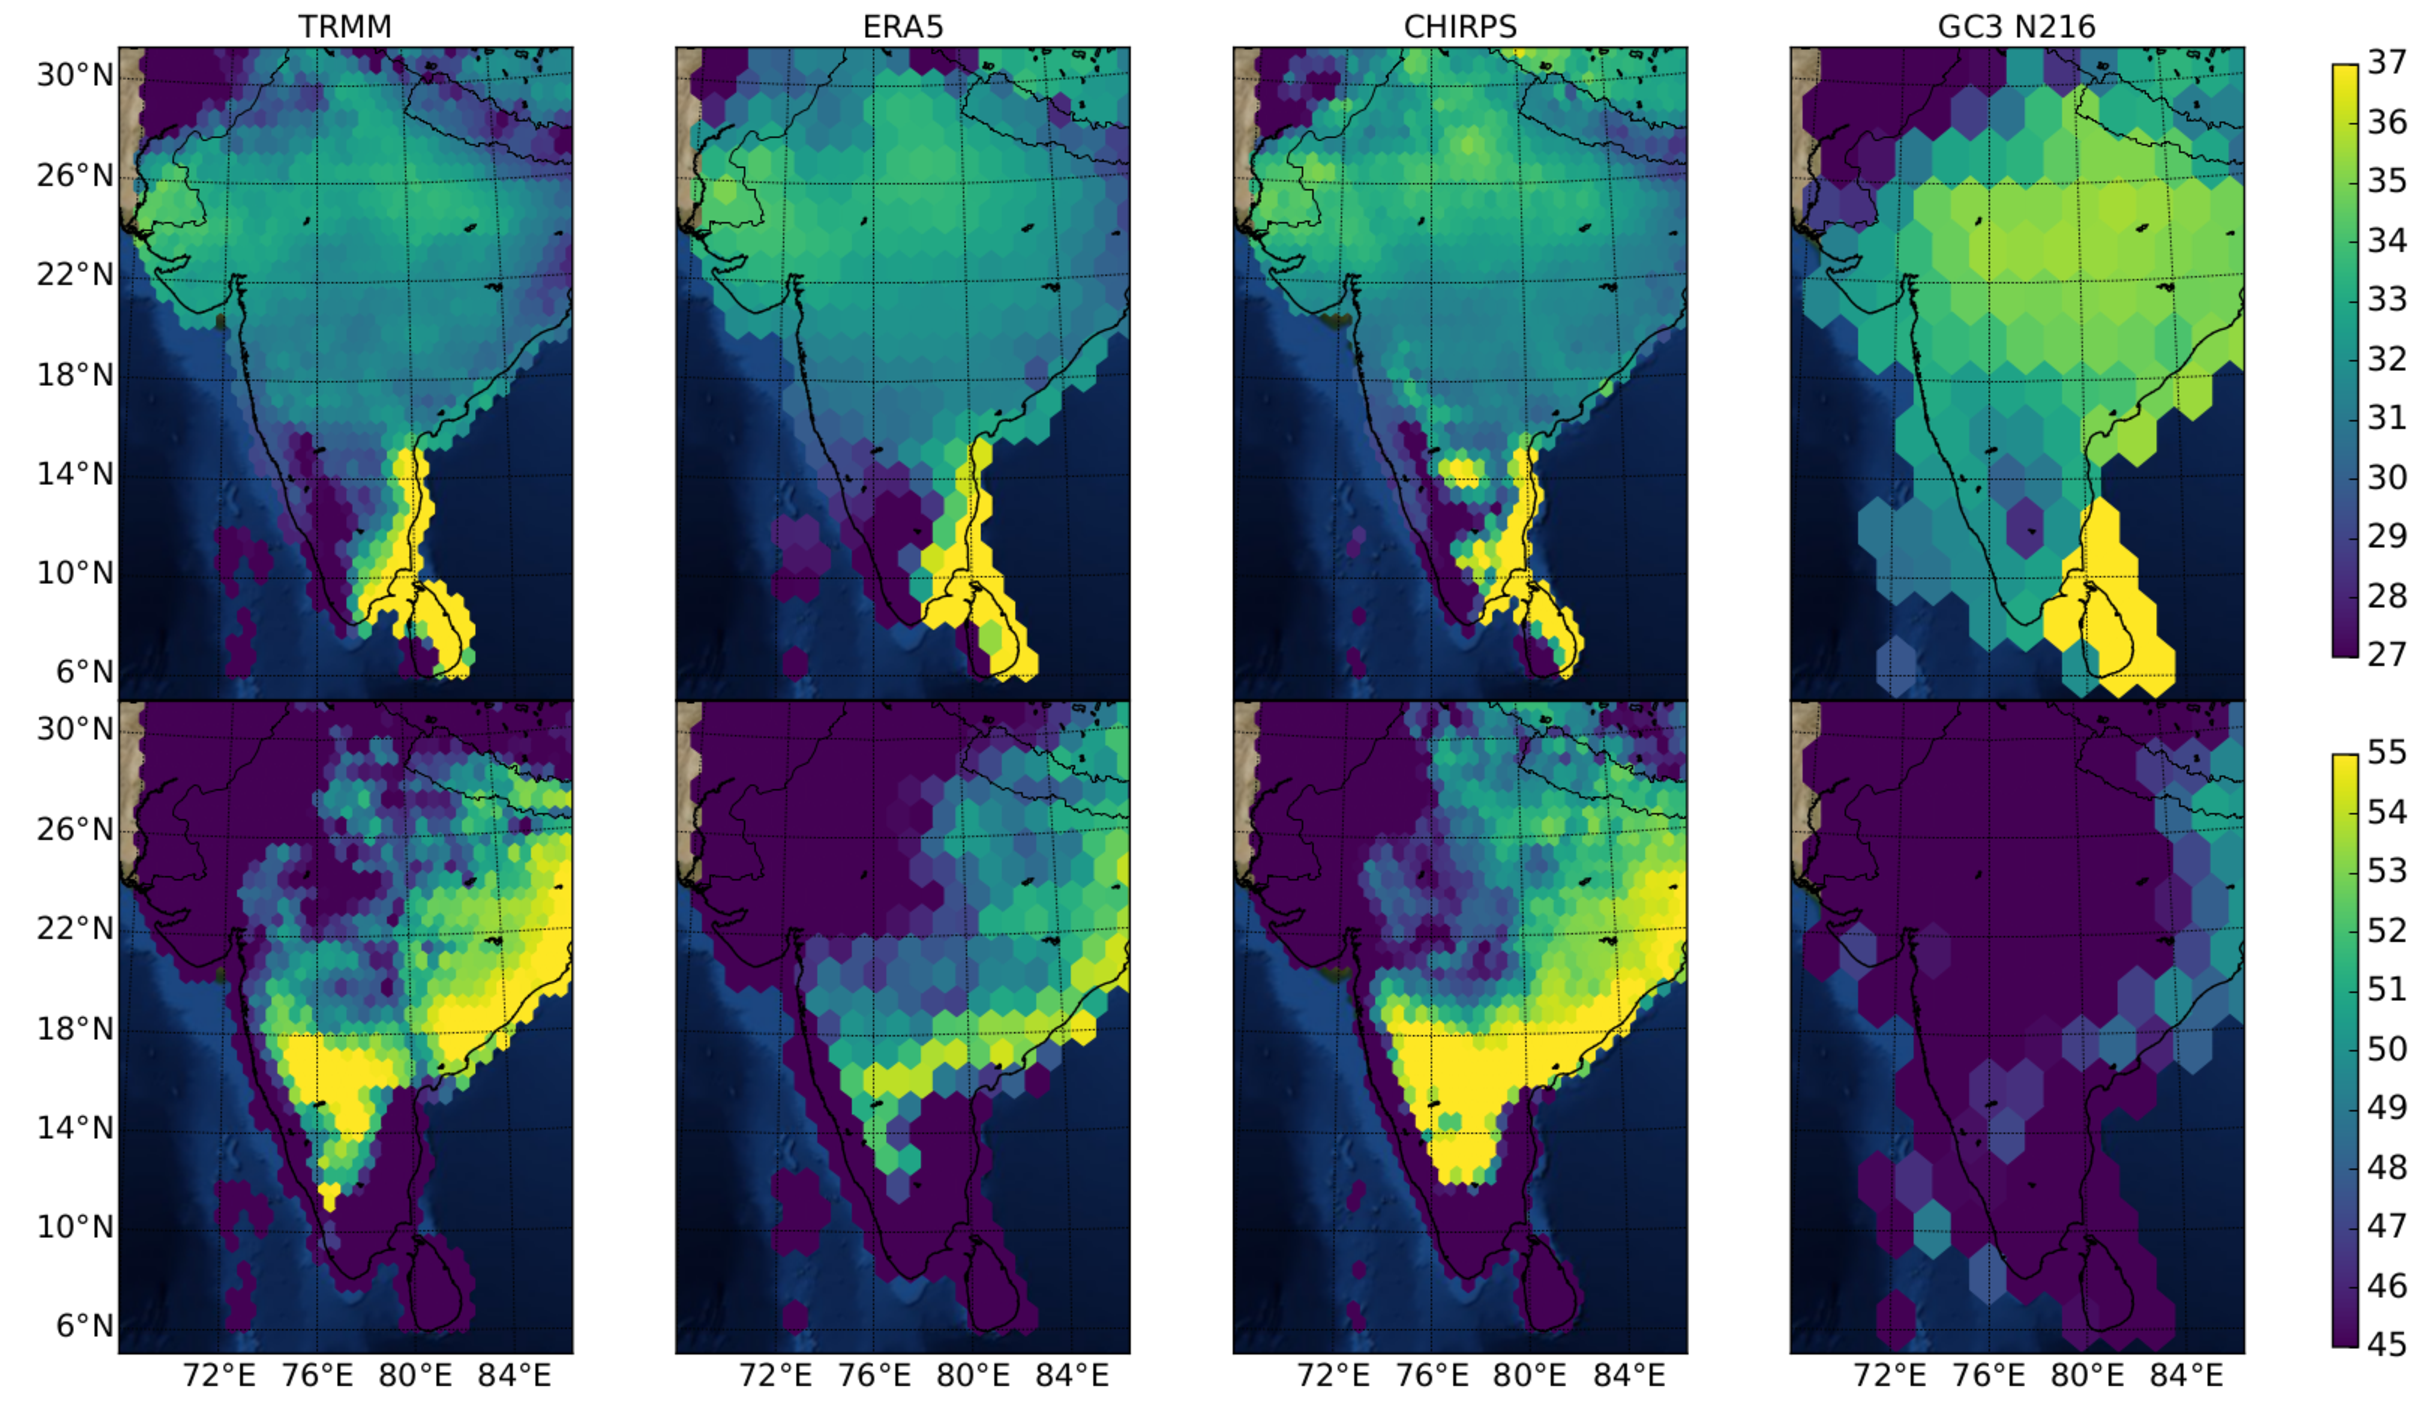
\includegraphics[width=\linewidth]{figures/wav_fig9.pdf}
\caption[Onset and retreat dates spatial distribution in Indian monsoon]{ As in Figure \ref{fig:wav_fig6} but for the Indian Monsoon.  }
\label{fig:wav_fig9}
\end{figure}

The spatial distribution of the mean onset and retreat dates of the Indian monsoon as characterized by the WT method (Figure \ref{fig:wav_fig9}) shows that the mean onset and retreat dates vary greatly spatially on the southern tip of the subcontinent. While most of northern India has a mean onset date around pentad 33, the western coast shows an earlier onset by about one or two pentads. There is high agreement in the onset date between the three observational datasets and the reanalysis over mainland India and between TRMM and ERA5 over the western coast of India. The earliest onset is found on the western coast around pentad 25-27 and extending to central India by pentad 31. 
The GC3 N216 simulation, however, shows a later onset than observed by about two pentads in most regions. In contrast, the spatial pattern for the mean retreat date shows higher spatial variability between the western and eastern coasts of India. CHIRPS shows the latest retreat dates over the south-central states when compared to TRMM and ERA-5. 

\subsection{The midsummer drought}

\begin{table}
% table caption is above the table
\caption{Mean pentads of monsoon onset (MO), rainfall retreat (MR), MSD Onset (MSDO) and MSD End (MSDE) in the MSD region [11-19$^\circ$N, 95-85$^\circ$W, illustrated in Figure \ref{fig:wav_fig11}a.] estimated through the WT method. Pentad 35 corresponds to the period between June 22-27 and pentad 52 to the period Sep 13-18. The model dates shown in bold are statistically different from CMAP and CHIRPS results to the 99\% confidence level according to a Welch's t-test. }
\label{tab:4}       % Give a unique label
% For LaTeX tables use
\begin{tabular}{p{2cm}p{1.5cm}p{1.5cm}p{1.5cm}p{1.5cm}p{1.75cm}p{1.75cm}}
\hline\noalign{\smallskip}
Dataset & MO & MR & MSDO & MSDE & coef1 & coef2  \\ \hline
TRMM & 25.8 [$\pm$2.2] & 61.6 [$\pm$3.1] & 35.9 [$\pm$2.4] & 49.0 [$\pm$4.1] & -9.5 [$\pm$4.2] & 10.4 [$\pm$5.4]  \\
CMAP & 26.7 [$\pm$1.9] & 60.6 [$\pm$3.3] & 36.5 [$\pm$2.6] & 48.0 [$\pm$4.2] & -7.1 [$\pm$4.2] & 7.7 [$\pm$4.3]  \\
CHIRPS & 26.7 [$\pm$2.3] & 61.4 [$\pm$3.1] & 36.5 [$\pm$2.7] & 48.3 [$\pm$3.5] & -4.7 [$\pm$2.7] & 5.5 [$\pm$3.2]  \\
ERA-5 & 26.5 [$\pm$2.2] & 61.8 [$\pm$3.2] & 36.1 [$\pm$2.7] & 48.8 [$\pm$3.5] & -10.7 [$\pm$5.4] & 11.8 [$\pm$6.6]  \\
UKESM-pi & 27.4 [$\pm$2.4] & 61.9 [$\pm$3.2] & \bf{38.2} [$\pm$2.7] & \bf{49.1} [$\pm$2.7] & -18.2 [$\pm$8.7] & 14.6 [$\pm$8.0]  \\
GC3 N96-pi  & 26.9 [$\pm$2.6] & 62.3 [$\pm$3.5] & \bf{37.8} [$\pm$2.1] & \bf{49.9} [$\pm$3.1] & -21.7 [$\pm$9.4] & 16.8 [$\pm$8.0]  \\
GC3 N216-pi  & 26.9 [$\pm$2.3] & 62.2 [$\pm$3.5] & \bf{38.4} [$\pm$2.1] & \bf{50.0} [$\pm$2.7] & -23.5 [$\pm$8.0] & 14.1 [$\pm$6.7]  \\
GC3-hist & 26.9 [$\pm$2.7] & \bf{62.8} [$\pm$3.7] & \bf{37.8} [$\pm$2.4] & \bf{50.3} [$\pm$2.6] & -19 [$\pm$8.7] & 17.1 [$\pm$8.4] \\
UKESM-hist & \bf{28.5} [$\pm$2.7] & \bf{62.8} [$\pm$3.5] & \bf{38.7} [$\pm$2.8] & \bf{50.1} [$\pm$2.7] & -20.3 [$\pm$10.1] & 14.9 [$\pm$8.3]  \\
%\noalign{\smallskip}\hline\noalign{\smallskip}
%number & number & number \\
%number & number & number \\
%\noalign{\smallskip}\hline
\end{tabular}
\end{table}

\begin{figure}[t!]
\centering
 %\noindent
 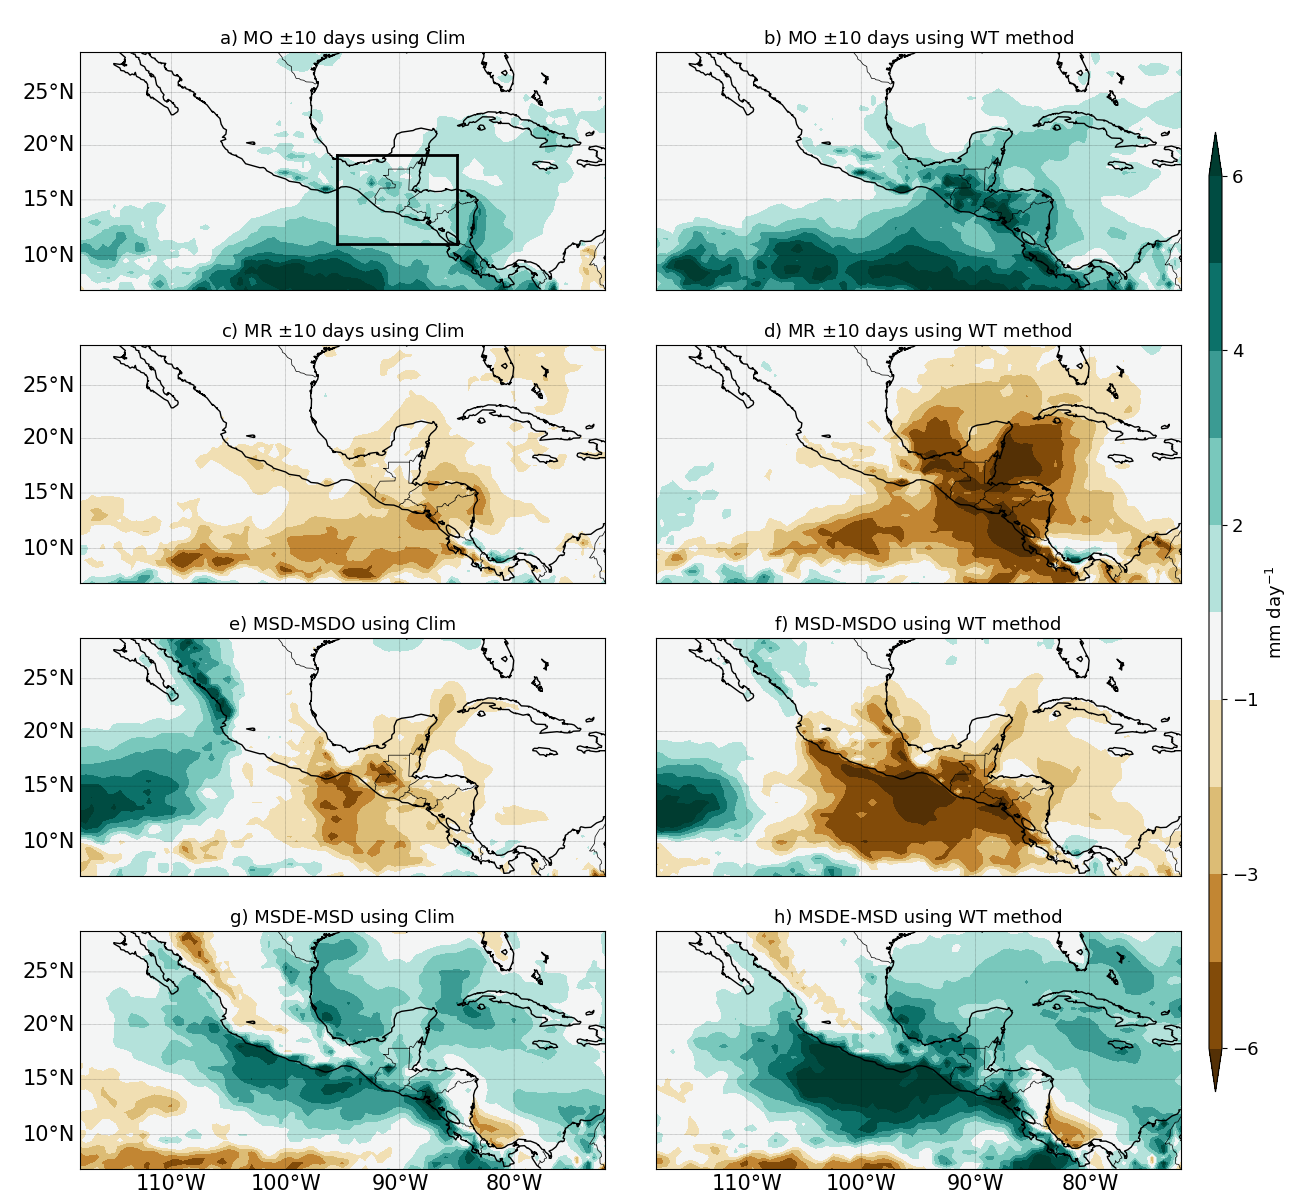
\includegraphics[width=0.95\linewidth]{figures/wav_fig10.png}
\caption[Precipitation anomalies after MSD]{  Precipitation anomalies for (a, b) the difference between the 10 days after monsoon onset and 10 days prior to onset (MO) using (a) the climatological dates of onset and (b) the dates estimated using the WT method. (c, d) are as in (a, b) but for monsoon retreat. (e, f) Difference between the Midsummer Drought (MSD) and the 10-day mean prior to the onset of the MSD (MSDO). (g, h) as in (e, f) but showing the difference between the end of the MSD (MSDE) and MSD. The data and calculations are from ERA-5. The black rectangle in a) shows the MSD area used to average the precipitation throughout this study.}
\label{fig:wav_fig11}
\end{figure}

Results from the application of the wavelet transform to the MSD, including the mean onset and retreat dates as well as the start and end dates of the MSD period, are reported in Table \ref{tab:4}.
The mean onset date in the observations is around pentad 27 (May 14), whereas the retreat date is around pentad 61 (October 31).
The end of the so-called first-peak period, or start of the relatively drier period (MSD), referred to in this thesis as MSD onset (MSDO) is consistently found in all the observed datasets to be around pentad 36 (around June 29).
The end of the drier period or start of the second peak, referred to in this thesis as MSD end (MSDE) is also consistently determined to be between pentads 48 to 49 in the four observational datasets.
In other words, the MSD has a mean duration of 12 pentads, or around two months, from late June to late August.
In the MOHC simulations, the MSD starts slightly later than observed by about two pentads, and ends about one pentad later than observed around September 10.

\begin{figure}[t!]
 \noindent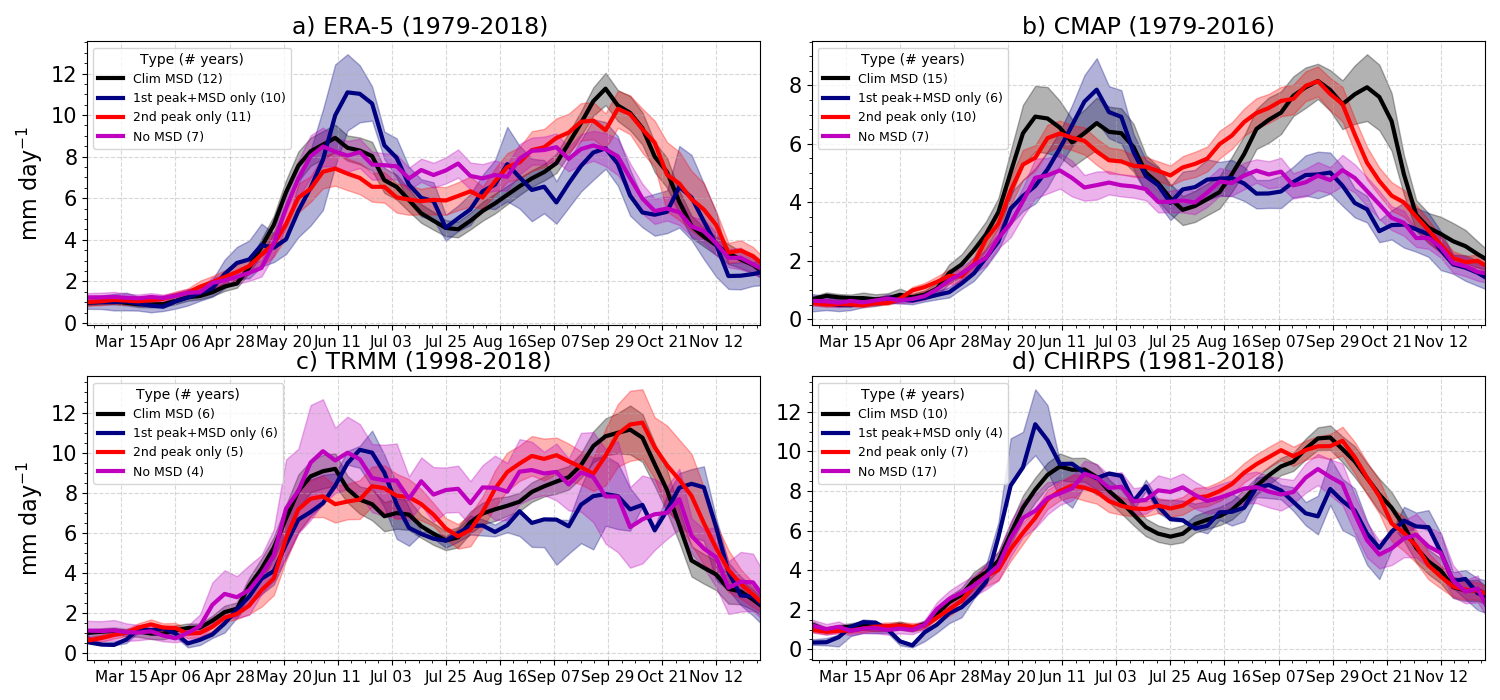
\includegraphics[width=\linewidth]{figures/wav_fig5c.png}
\caption[Seasonal cycle of precipitation for various MSD categories]{ Pentad-mean precipitation in years differentiated by MSD characteristics in four datasets: (a) ERA-5, (b) CMAP, (c) TRMM and (d) CHIRPS. The shading for each line represents first to third quantile of the distribution provided a bootstrapping with replacement all the years in each composite 10000 times.  }
\label{fig:S2}
\end{figure}
%\clearpage

Figure \ref{fig:wav_fig11} shows the rainfall anomalies associated with the different periods (stages) of the rainy season in southern Mexico and Central America. These include monsoon onset and retreat, and the start and end of the MSD, the MSDO and MSDE, respectively. For each stage, we compared the anomalies computed by separating the stages using the WT method or the dates of the climatological monsoon onset, retreat, MSDO and MSDE as found in Table \ref{tab:4}. In this way, the ability of the WT method to characterise rainfall variations is tested against a first best guess -- the climatological mean dates. 

Overall, using the dates for MSDO and MSDE from the climatological dates results in weaker anomalies than compositing via the specific dates for each year obtained with the WT method.  Even though the area-averaged signal used to diagnose the different MSD stages focuses on a small region of southern Mexico and northern Central America, the anomalies associated with the onset and end of the MSD (Figures \ref{fig:wav_fig11}f, h) extend across the East Pacific warm pool, most of the western coast of Mexico and into to the Caribbean Sea and Cuba. This result suggests that the MSD is part of a regional-scale process on the result of local-scale processes. 

The analysis of individual years of observed precipitation in the selected area-averaged time-series showed that not all years showed a bimodal signal in the area-averaged precipitation (Fig. \ref{fig:S2}). In fact, a given year could be classified as having (1) a canonical two-peak structure separated by an MSD, (2) only having a first peak and an MSD but no second peak, (3) only having a second peak but no clear MSD or (4) a plateau-like monsoon season with no MSD-type variations (see Fig. \ref{fig:S2}). 


Due to this year-to-year variability in the characteristics of the seasonal cycle, an objective measure was defined to determine whether a signal presented a robust MSD-bimodal seasonal cycle.  
For this purpose, the WT algorithm was applied to randomly generated precipitation time-series.
 The random time-series are constructed by randomly sampling observations in the wet and dry seasons. 
 The pentad-mean onset and retreat dates from Table \ref{tab:4} were used to composite the observations into dry and wet distributions. 
 
 
 For a random time-series that aims to mimic one year of precipitation, the rainfall values for each pentad in the year are randomly selected from the dry or wet distributions, depending on the pentad. In this way, the value of a given pentad of the random time-series may have been observed at a different pentad; the only constraint is that the random values come from pentads that were observed in the same season: dry or wet. The logic behind this approach is that in most monsoon regions, the peak monsoon rainfall should follow a plateau, see for example the North and South American monsoons in Figure \ref{fig:8} in the previous chapter. However, a bimodal regime would show a notable decrease in precipitation in the middle of the rainy season, such that it cannot be explained by the inherent short-scale variability of rainfall. 
 
\begin{figure}[t!]
\centering
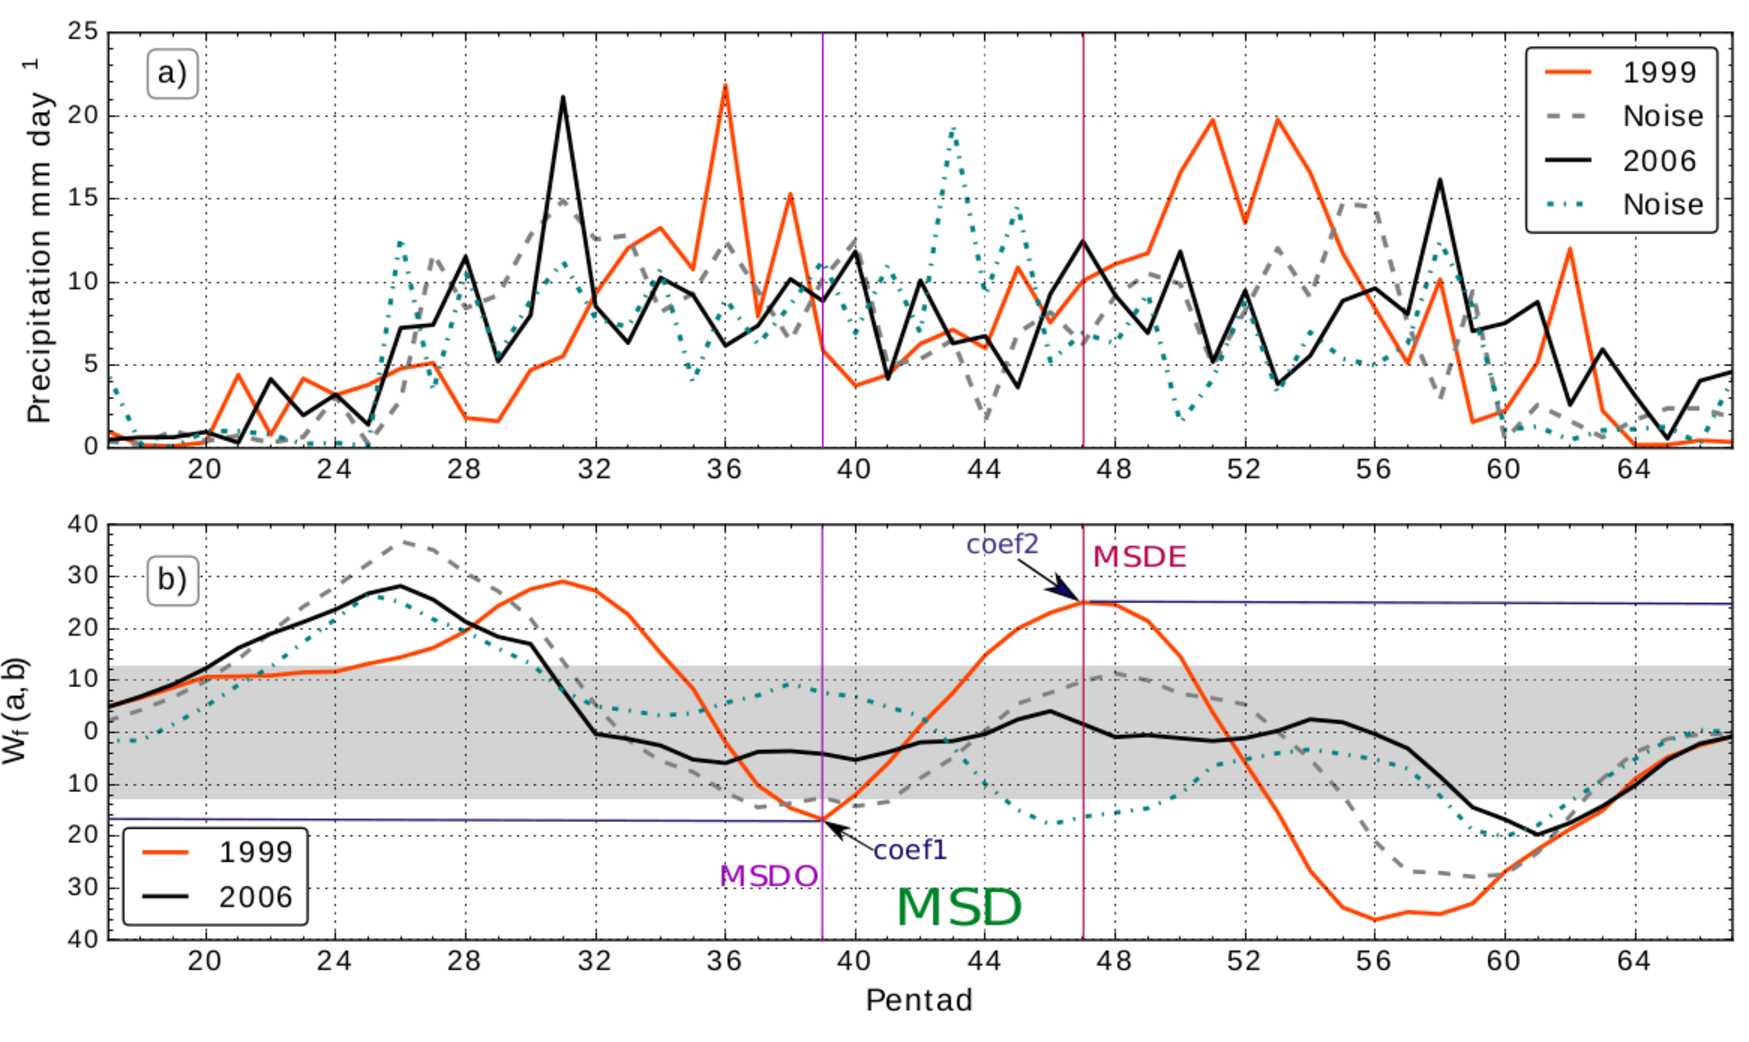
\includegraphics[width=\linewidth]{figures/wav_S1.pdf}
\caption[Determination of MSD timings and coefficients]{(a) Pentad-mean precipitation in two years of TRMM data: 1999 and 2006 and two randomly generated precipitation time-series (see text). (b) Sum of the wavelet transforms of the time series in (a). The shaded region in gray in (b) corresponds to the interval between the first quantile of $coef1$ and the third quantile of $coef2$ of 10,000 random timeseries constructed with TRMM data. The onset (MSDO) and end (MSDE) of the relatively drier period, as well as the location and values of $coef1$ and $coef2$ for 1999 are labelled in (b). }
\label{fig:S1}
\end{figure}
 
 
 This approach has two advantages. First, that the random time-series impose a monsoon-like feature with a sharp wet-dry season contrast but secondly, the random selection in the wet season removes the possible signal of the MSD in the climatological rainfall.
 The random time series are then constructed by randomly drawing values at each pentad  from the wet or dry season distributions of each dataset.
 Then, the WT method was used on 10,000 of these random-time series. This approach rendered a distribution of coefficients ($coef1$ and $coef2$) essentially representing the variability of the WT method applied to noise.
 
  Figure \ref{fig:S1} shows the pentad-mean time-series from two years in the TRMM dataset, and two randomly generated time-series.
The coefficients $coef1$ and $coef2$, illustrated in Figure \ref{fig:S1}b, measure the difference in precipitation between the first peak and the MSD period and the MSD and the second peak, respectively. The first quantile of $coef1$ and the third quantile of $coef2$ provide a measure of robustness for the observed $coef1$ and $coef2$. In other words, for a year to be classified as having a robust MSD signal, the resulting $coef1$ and $coef2$ of the WT procedure must be lower and higher, respectively, than those obtained for a random time-series.
The analysis of $coef1$ then determines the existence of a first-peak MSD type variability and $coef2$ determines the robustness of a possible second-peak for that year.
By this procedure, a given year could fit into four categories:

\begin{itemize}
\item Canonical MSD: $coef1$ lower than the first quartile (25\%) of random $coef1$ and $coef2$ higher than the third quantile (75\%) of random $coef2$.
\item 1st peak+MSD: $coef1$ lower than the first quartile of random $coef1$ but $coef2$ lower than the third quartile of random $coef2$. In other words, the second peak is not distinguishable from noise.
\item 2nd peak only: $coef1$ higher than the first quartile of random $coef1$ but $coef2$ higher than the third quartile of random $coef2$. In other words, the second peak is distinguishable from noise, but there is no first-peak + MSD structure.
\item No MSD: $coef1$ higher than the first quartile of random $coef1$ and $coef2$ lower than the third quartile of random $coef2$. In other words, the precipitation time-series shows no robust signal of an MSD regime, with a first or second peak.
\end{itemize}
 
\begin{figure}[t!]
\centering
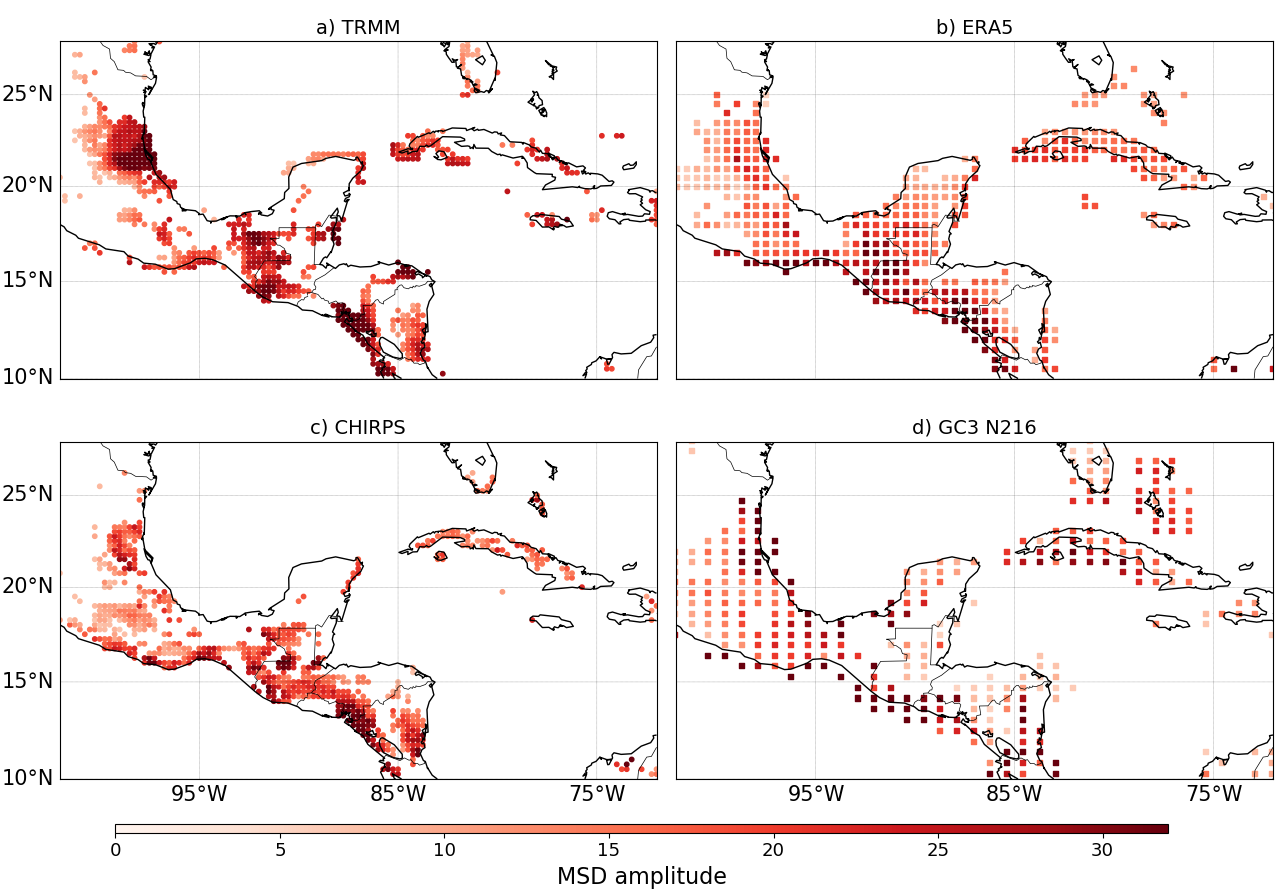
\includegraphics[width=\linewidth]{figures/wav_fig12.png}
\caption[Map of MSD significant regions]{Grid points where the MSD is significantly different, i.e.\, outside the first and second quartiles of the random distribution, from noise (see section 3.3) for a) TRMM, b) ERA-5, c) CHIRPS and d) GC3 N16-pi.  The magnitude of the MSD, measured as $coef2-coef1$ is shown in colour shading.  }
\label{fig:wavfinalmap}
\end{figure} 
 
 Figure \ref{fig:S2} shows how separating years into these categories affects the pentad-mean seasonal cycle of precipitation in southern Mexico and Central America in four observational datasets. This figure also validates the above procedure as the WT method is able to robustly separate years into the different categories. 


For each dataset we determine those grid-points showing a robust MSD. We use the method outlined above to construct the random time-series for each grid-point and estimate the random values of $coef1$ and $coef2$, repeating the procedure 10,000 times. A given grid-point is diagnosed to have a robust MSD when the value of $coef2-coef1$ is higher than the third quartile of the PDF of the random time series. The value of $coef2-coef1$ is a measure of the magnitude of the MSD since $coef2$ measures the relative strength of the second-peak compared to the MSD and therefore positive in an MSD grid-point and $coef1$ compares how dry the MSD is relative to the first-peak and thus negative if an MSD regime is observed at that grid point. 

\begin{figure}[t!]
\centering
 %\noindent
 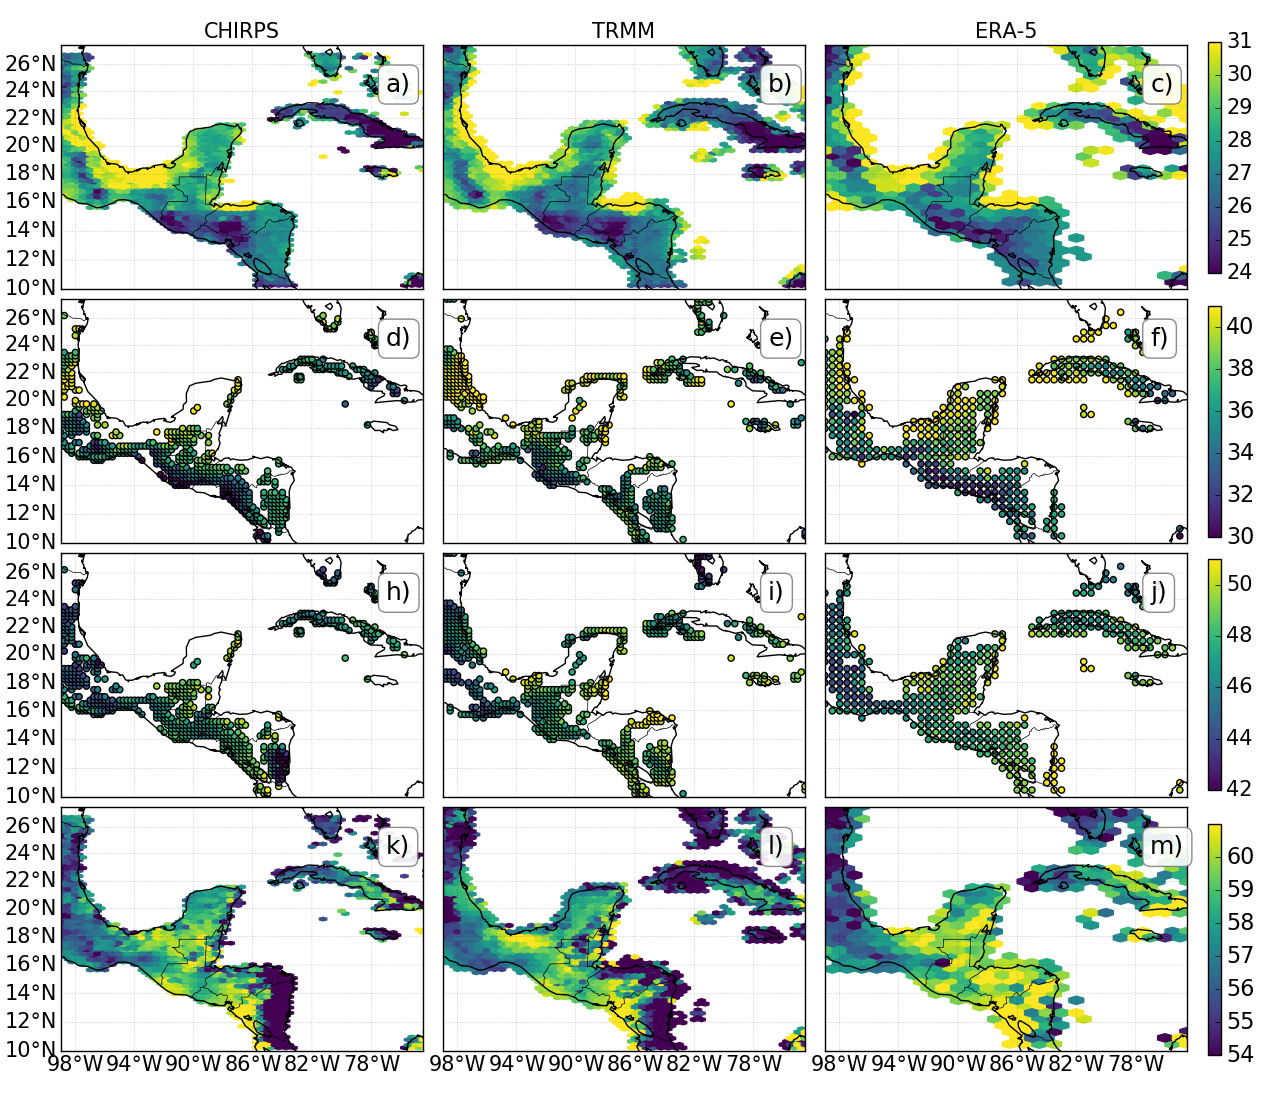
\includegraphics[width=\linewidth]{figures/wav_fig13.png}
\caption[Spatial distribution of MSD timings]{  Spatial distribution of pentad dates of the timings of the summer rainfall season in the MSD region, showing (a-c) MO dates and (d- f) MSDO dates, (g-i) MSDE and (j-l) MR for (left) CHIRPS, (middle) TRMM and (right) ERA-5. }
\label{fig:wav_fig13}
\end{figure}


Figure \ref{fig:wavfinalmap} shows the regions where the climatological rainfall shows a MSD signal that is distinguishable from noise, i.e., regions where the values of $coef2-coef1$ exceed the third quartile of the distribution composited with random time-series, as well as the magnitude of the MSD for the TRMM, ERA5, CHIRPS and the GC3 N216 piControl simulation. Cuba, western Central America and most of southern and central-eastern Mexico exhibit a robust MSD signal. 
This map also shows that the strongest MSD signal is found on the western coast of northern Central America and northeastern Mexico. 
The high correspondence between the three observational datasets shows that the method is robust across datasets. These results agree well with previous studies on the spatial distribution of the MSD \citep{magana1999,perdigon2018,anderson2019multiscale,zhao2021}. In particular, the method is able to replicate the previously reported MSD signal in the Pacific Mexican coast and the stronger MSD signal in northeastern Mexico.  



Figure \ref{fig:wav_fig13} shows the spatial distribution of the mean onset and retreat pentads and the start and end of the MSD, in the grid-points where the signal is significant as in Fig. \ref{fig:wavfinalmap}. The earliest rainfall onset is found on the western coast of southern Mexico, Guatemala and El Salvador, as well as in Cuba, at pentad 25, whereas onset in the Yucatan peninsula is found at pentad 28 and even later, around pentad 31, in the eastern states of Mexico. In contrast, the retreat date seems spatially more homogeneous as northern Central American has a mean retreat date around pentad 59 and central Mexico around pentad 54.
The MSD coherently starts over the western coast of Guatemala and Chiapas around pentad 33. In contrast, the MSD on the eastern Mexican states of Veracruz and Campeche begins after pentad 40. The earliest MSD end (Figs. \ref{fig:wav_fig13}h-j) is found in central and northeastern Mexico, around pentad 42 whereas the MSD in Guatemala ends around pentad 48.



\section{Summary and discussion}

The assessment of the AMS in the MOHC submissions to CMIP6 in Chapter \ref{ch:4-ams} lacked a robust analysis of the representation of the timings of the monsoon. 
The principal reason for this shortcoming was the lack of a robust, wide-spread method to diagnose onset and retreat dates in the various regions of the AMS with the various datasets available. This chapter aimed to address this issue by developing a new method to compute onset and retreat dates for the purpose of intercomparison between multiple observational and model data.

The novel method described in this chapter uses pentad-mean precipitation data to compute a wavelet transform over multiple temporal scales from which a set of coefficient and diagnostics are used to determine onset and retreat dates. The wavelet function used is the Haar wavelet, a wavelet typically used to find abrupt changes in signals.
Onset is defined as the maximum of the sum of the coefficients of the wavelet transform computed over a range of temporal scales or dilations. These dilations were found to provide the best results in a range from 28 to 54 pentads. Monsoon retreat is similarly defined but using the minimum of this sum of wavelet transform coefficients. The use of this method is illustrated using multiple observational datasets and climate model output. The method is compared to existing methods to find onset and retreat dates in three monsoon regions.

The method performs favourably to existing methods that use precipitation thresholds in the North American Monsoon, as shown by the anomalies of precipitation, wind and geopotential around the onset and retreat dates. 
The spatial distribution of monsoon onset and retreat in this region was found to be sensibly captured by the wavelet algorithm, illustrating the earlier onset in central western Mexico and the later onset in northwestern Mexico, Arizona and New Mexico. 
The spatial distribution of onset and retreat dates was diagnosed to be very similar between the TRMM, CHIRPS and ERA5 datasets, which suggests that the method produces similar results in datasets with different resolutions and climatologies. This result also suggests that the method is robust to be used at the grid-box scale, and not just for region-averaged time-series.
 
The WT method also compares well to a hydrologically defined index (HOWI) in the Indian Monsoon, although the WT better captures the precipitation variations whilst HOWI betters captures changes to the moisture transport. However, the WT method is also able to capture strong differences in moisture transport around the onset and retreat dates, in both models and observations. The WT method obtains a later onset and retreat as compared to the HOWI index, which is possibly associated with a lag between the moisture transport about the Arabian Sea (as diagnosed by HOWI) and the precipitation over mainland India (as measured by the WT method). The spatial distribution of onset and retreat dates in the Indian Monsoon region, diagnosed using the WT method seems to be relatively consistent and coherent amongst the observational datasets, as the mean onset date in mainland India was found at pentad 32.
Onset is earliest on the western coast of India and the onset date appears to be very homogeneous in central India.

The WT method was extended to characterise the timings and strength of the Midsummer Drought (MSD), using the same principle as for determining onset in the Indian monsoon, but computing the WT over smaller dilations around the onset and retreat dates.  By using randomly-generated time-series, the spatial distribution of grid-points displaying a robust MSD signal was found in Cuba, the northwestern coast of Central America and several regions of south and north-eastern Mexico.  The MSD in southern Mexico and northern Central America is found to start around pentads 35 and 36 (last week of June) and end around pentad 48 (mid-August) in most observational datasets and the ERA5 reanalysis. To our knowledge, this extension of the WT method provides one of the very few methods for characterising the MSD on sub-monthly scales.
%This method may be potentially useful when diagnosing changes to the characteristics of the MSD in models or observations, as will be shown in the following chapter. 


%discussion on problems with thresholds, 
%area-mean average 
%Current methods that diagnose monsoon onset and retreat using pentad or daily-mean precipitation time-series are typically rigid threshold methods. These threshold methods depend on a number of parameters that need to be tuned for a specific monsoon region and for a specific dataset. 
%For instance, the method by \citetalias{geil2013} used a threshold value specific for the North American Monsoon and specific for the TRMM dataset but also to the limits of the area used for area-averaging the precipitation. In other words, the persistence and threshold values of most of the threshold methods require normalization, statistical treatment or additional tuning to the parameters to account for climatological differences in the datasets which introduces uncertainty. The method by \citetalias{arias2012} then uses a climatological mean value as the threshold, but in a climate model with a significantly positive bias in the dry winter season of a monsoon this method would be prone to error as the biased seasonal cycle may impose a biased calculation of monsoon onset and retreat. 

% different dataset climatology, characteristicis
% model climatology and biases. 
% window and persistence parameters vary monsoon region to another.


The WT method is in many ways similar to the agronomical and threshold methods \citep[e.g.][]{liebmann2001interannual,moron2014interannual}, as the implementation of the method uses a subjective determination of the dilation scales; these scales are comparable to the persistence and window parameters of the threshold methods. However, the WT method presented has three main advantages over most threshold methods. First, the method produces robust results for the Indian and North American monsoon of onset and retreat, and spatial distributions comparable to previous methods \citep{moron2014interannual} while not being subject to 'false-hits' nor years without an identification of the onset and retreat dates. In other words, the method provides robust results without requiring further treatment of years with false-hits or undetermined years. 

The second advantage of the method is portability, or utility, as the method shows robust and consistent results for three observational datasets, a reanalysis and climate model experiments with varying climate forcing but without any constraint or treatment of the data beforehand and in three different regions with different seasonal cycles. In other words, this method is robust across datasets and regions. In contrast to rigid threshold techniques \citep[e.g.][]{liebmann2001interannual}, the identification of onset and retreat for each time-series, e.g. at each grid-point, is based upon coherent temporal changes within each precipitation time-series while not using parameters determined 'a priori' specifically for a region. The WT method then, can be used in any time-series, regardless of the origin of the time-series, without any further change or consideration than those established by the dilations scales determined in section 2.2.1. 
The portability of the method also means that the method can be implemented as a 'local-scale' method applied at the grid-box scale for high-resolution datasets such as CHIRPS as well as for regional scales using area-averaged time-series.

Third, and in contrast to typical threshold methods, the wavelet method can be applied to climate model output straightforward using the same configuration of dilation scales, a feature of the method that is illustrated by our analysis of several experiments using the Hadley Centre models. The treatment of the data does not require  any normalisation or statistical treatment even when used for grid-point time-series for different regions or experiments with varying forcing where the seasonal cycle or total annual rainfall may change notably within the model time-series.


This chapter follows up on some missing details of the previous chapter by analysing the timings  of the North American monsoon and the Central American MSD in the MOHC models by objectively computing the onset and retreat dates with the WT method. The results confirm that the CMIP6 MOHC models reasonably simulate the seasonal cycle of rainfall in North American monsoon and the MSD regions.
Moreover, this chapter provides the main tool to be used in the following chapter, which aims to better understand the physical mechanisms behind the MSD, a question that would be difficult to address without the existence of a robust method for determining the timings of the MSD on the pentad-scale.

\begin{savequote}[8cm]
Alles Gescheite ist schon gedacht worden.\\
Man muss nur versuchen, es noch einmal zu denken.

All intelligent thoughts have already been thought;\\
what is necessary is only to try to think them again.
  \qauthor{--- Johann Wolfgang von Goethe \cite{von_goethe_wilhelm_1829}}
\end{savequote}

\chapter{\label{ch:2-litreview}On the dynamical and thermodynamical mechanisms of the MSD in the Met Office CMIP6 models}

\minitoc


The MSD has relevant implications to farmers in Central America, who are subject to climatic stress due to droughts and are thus affected by the MSD, which is coloquially referred to as 'El Veranillo' in Central America and 'can\' icula' in southern Mexico because the drier period  coincides with the Canis Major constellation appearing in the sky \citep{dilley1996}. In the context of climate change, farmers are already perceiving and having to adapt to changes in the characteristics of the rainy season, such as the timing and strength of the midsummer drought \citep{hellin2017,de2018,harvey2018}. Various communites across country borders have identified and experienced the MSD, which has different names, known as 'El Veranillo' in Central America and because the drier period typically coincides with the Canis Major constellation apearing in the sky, the MSD is also referred to as 'can\' icula' in some regions \citep{dilley1996}.  

This section introduces the main features of the regional climate of Mexico, Central America and the Caribbean. A summary is presented of the literature on the mechanisms that drive the variations of rainfall. The spatial and temporal characteristics of the MSD are also analysed in reanalysis and observations and in HadGEM3 and UKESM1.

\section{Climatological features}
\label{sq:msdclim}
 \begin{figure}[t!]
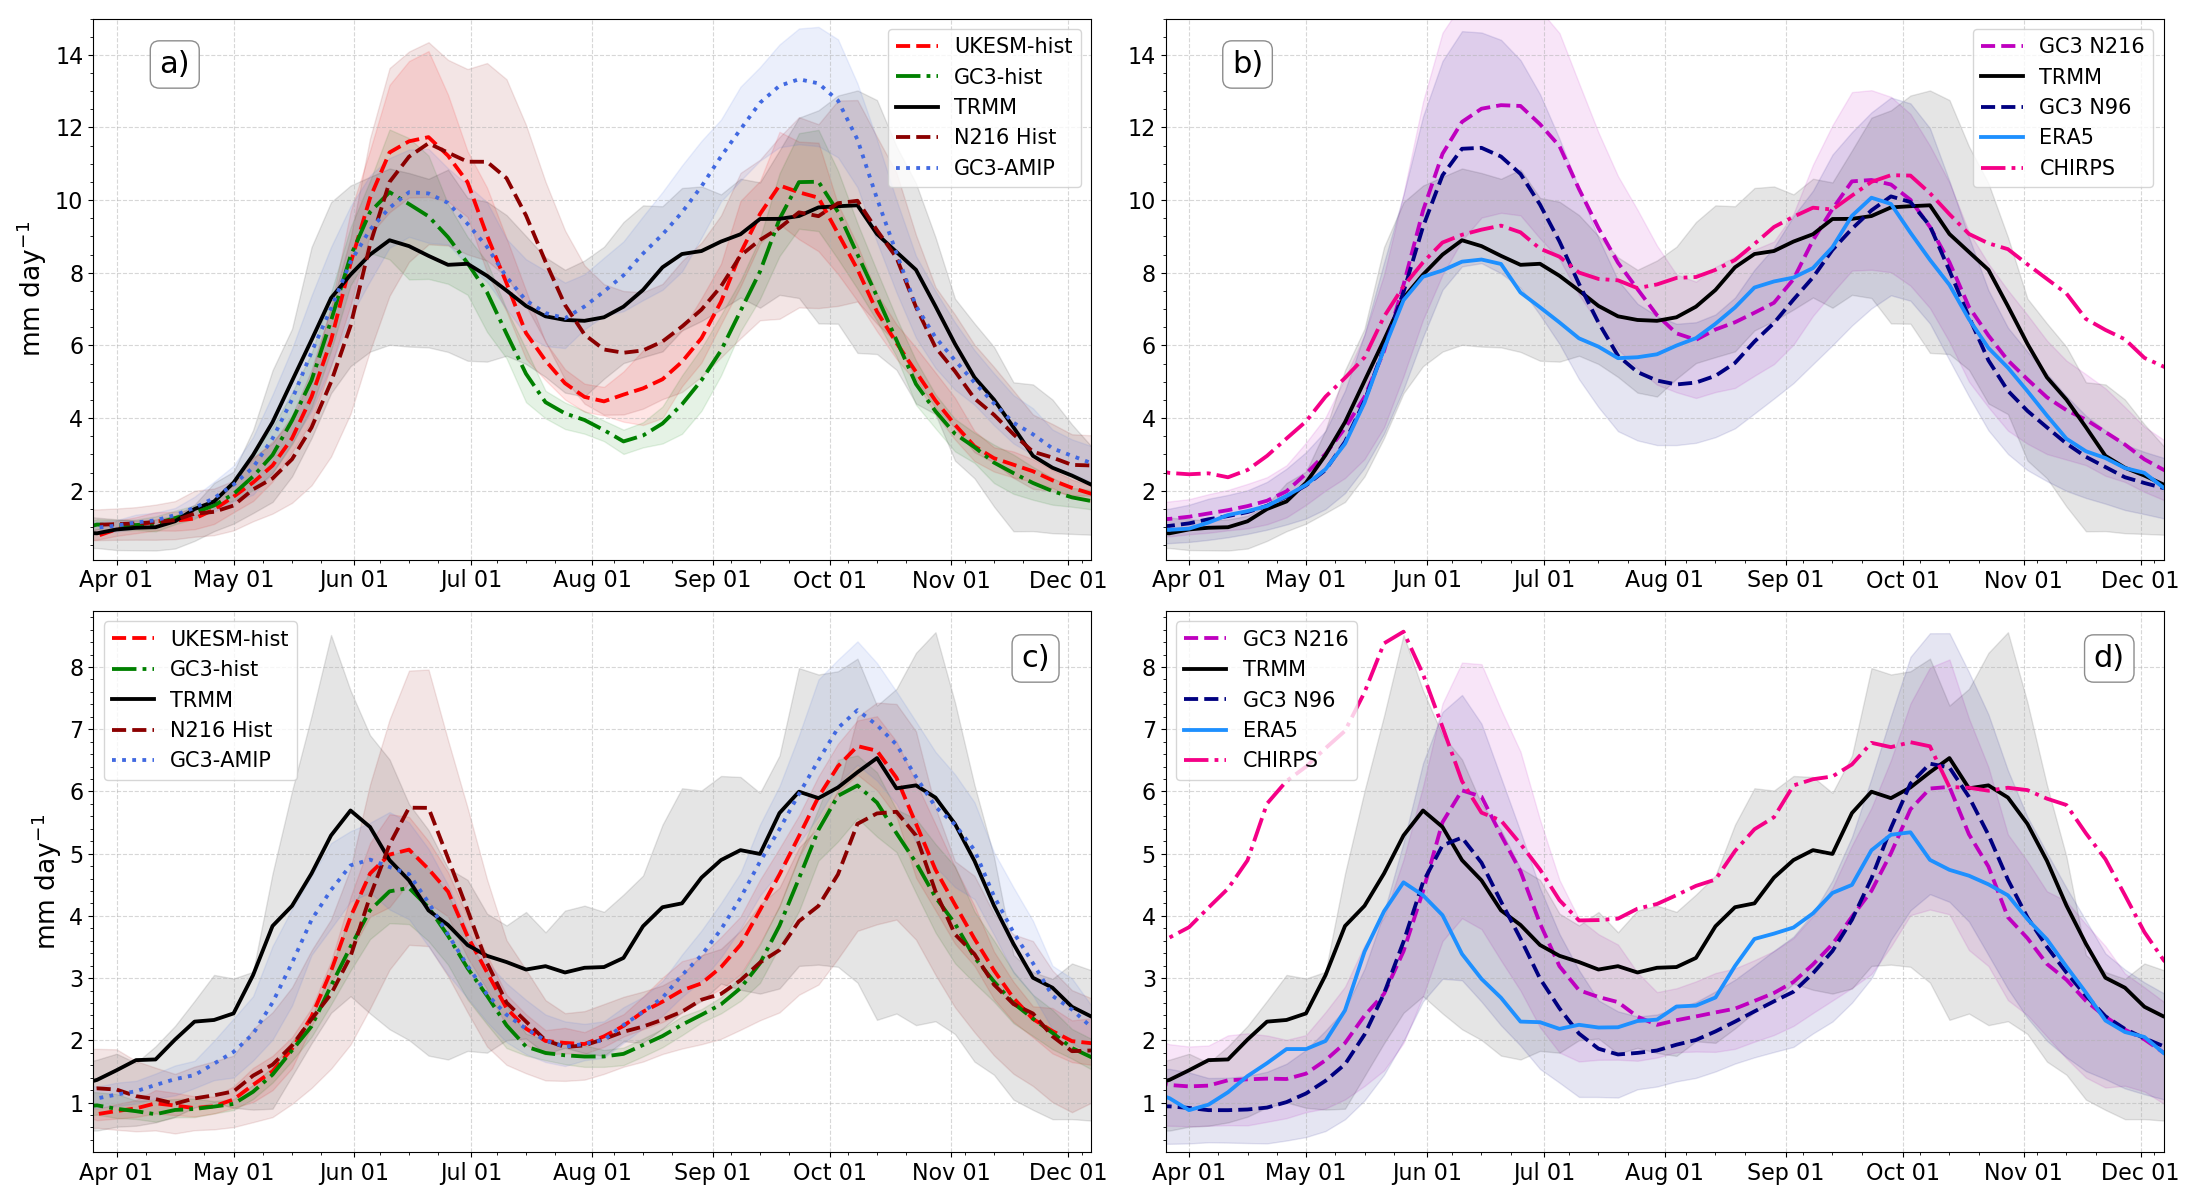
\includegraphics[width=\linewidth]{figures/pmean_f.png}
\caption{Pentad-mean precipitation in (a, b) southern Mexico and northern Central America and (c,d) Cuba. Shading shows uncertainty obtained by bootstrapping or ensemble spread. }
\label{fig:msdcaribb}
\end{figure}

Figure \ref{fig:msdcaribb} shows the pentad-mean seasonal cycle of precipitation in Central America and the Caribbean. The seasonal cycle in both regions follows that of a monsoon, i.e., a dry winter and a wet summer season. In the first region (Figures \ref{fig:msdcaribb}a, b), two precipitation maxima, in June and September, are separated by a decrease in precipitation during July and August, \textit{i.e} the MSD. In Central America, the difference between the first peak (June 15) to the driest pentad of the MSD (Aug 01) is of about 2 mm day$^{-1}$, according to TRMM. 
 The two peak structure in the Caribbean (Figures \ref{fig:msdcaribb}c, d) is characterised by two peaks in May and October with a four-month drier period in between the two peaks  \citep[e.g.][]{giannini2000,gamble2008,angeles2010origins}. In Cuba, the difference between the first peak (June 01) to the driest pentad of the MSD (Aug 01) is of about 3 mm day$^{-1}$ in the TRMM dataset. 
 

 
 \begin{figure}[t!]
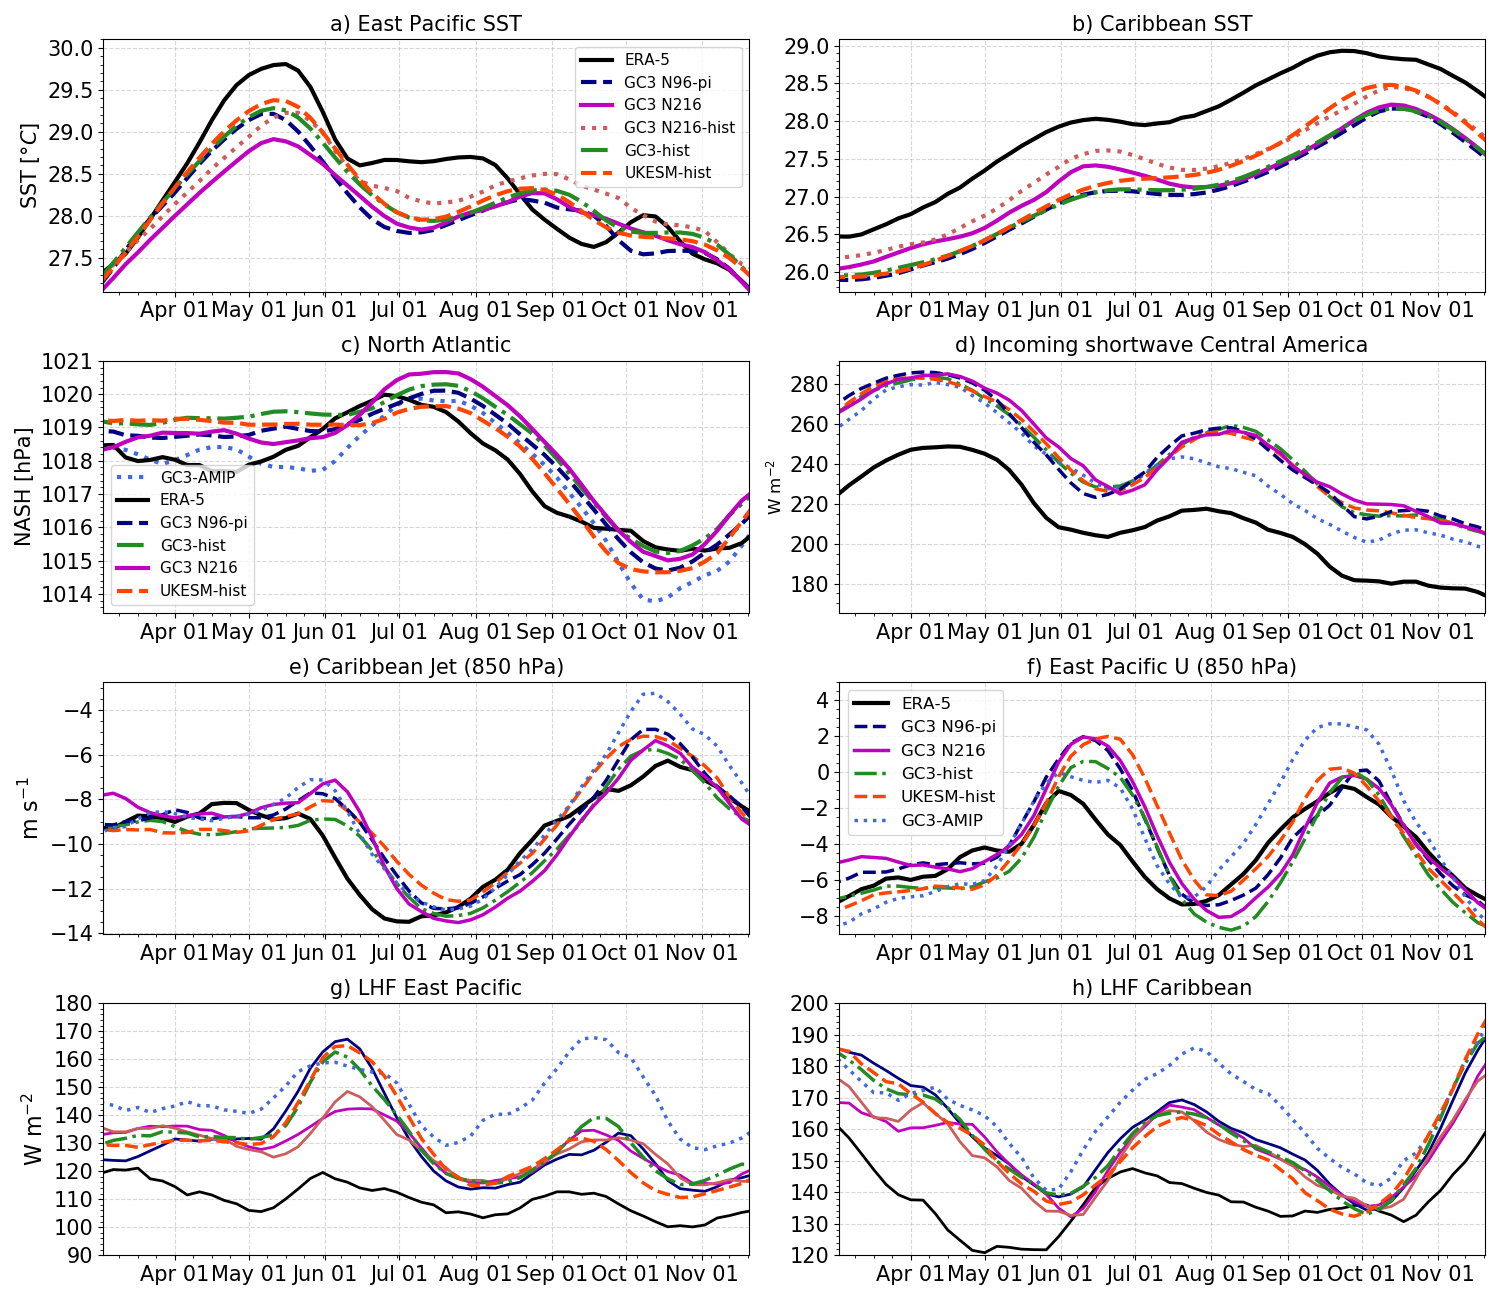
\includegraphics[width=\linewidth]{figures/CSST}
\caption{Pentad-mean seasonal cycle of indices associated with the MSD in Central America and the Caribbean.}
\label{fig:csst}
\end{figure}

Precipitation in these regions depends on several factors such as the seasonal migration of the East Pacific (EP) and Atlantic ITCZs. The SSTs in the Gulf of Mexico, the Caribbean Sea, the western tropical Atlantic and the Eastern Pacific are also very relevant for the seasonal cycle and interannual variations \citep{magana1999,amador2008,straffon2019}. Figures \ref{fig:csst}a, b show the seasonal cycle of SSTs in the EP and the Caribbean Sea. While the EP shows a maximum in SSTs in late May, during the early stages of the monsoon in Central America, the Caribbean SSTs peak in early fall, about five months later. 


%The CLLJ is a strong easterly low-level (925 hPa) that reaches maximum winds speeds of 12 $m\,s^{-1}$ on February and July 
The Caribbean Low-level Jet (CLLJ)is a strong low-level easterly jet in the Caribbean Sea that peaks at the end of June (Figure \ref{fig:csst}e) at the 925 hPa level \citep{amador2008,herrera2015,maldonado2016}. The CLLJ  determines the moisture transport from the Caribbean Sea into the eastern Pacific across the Central American landmass as well as the northward moisture transport into the Gulf of Mexico and Florida \citep{munoz2008,hidalgo2015,maldonado2016}.


%Figure \ref{fig:eof1} shows the climatological summer rainfall in the region and the difference in rainfall between the first peak and MSD and between the second peak and the MSD, characterised by the MSD-MSDO and MSDE-MSD differences. 
%Although the dates of the onset and end of the MSD determined using the WT method are defined using precipitation area-averaged over a relatively small region, the precipitation anomalies associated with the different stages of the seasonal cycle extend to most of Mexico and the Caribbean Sea and Gulf of Mexico. 
%For example, consider the MSDE-MSD differences in the CHIRPS dataset (Figure \ref{fig:eof1}i) where most of northern Central America, southern Mexico, the eastern coast of Mexico shows a positive (+5 mm day$^{-1}$) anomaly. In other words a large region experiences a relatively large increase in rainfall after the midsummer.

\section{Theoretical understanding of the MSD}\label{sq:lit}



Since the first observational descriptions of the MSD \citep[e.g.][]{mosino1966}, studies have aimed to explain the physical mechanisms responsible for causing the observed two-peak seasonal cycle of rainfall. However, 
in spite of extensive research \citep[e.g.][]{magana1999,giannini2000,gamble2008,ryu2014,herrera2015,maldonado2017,straffon2019}, debate remains over which is the leading-order mechanism that causes rainfall to decrease at midsummer and increase again at the end of the summer. Any complete theory or conceptual model must account for the following characteristics of rainfall in these regions. First, the processes that determine the strength of the first peak of rainfall. Second, the timing and strength of the MSD, i.e., what causes rainfall to decrease at midsummer. Finally, the theory must explain the timing and mechanism driving the second increase in precipitation after the midsummer. % why rainfall increases again at the end of the summer, the end of the MSD, and why this happens at this time of the year. 

Studies argue over the roles played by the Atlantic and EP Oceans, and the Caribbean Sea and whether the MSD is caused by two precipitation enhancing mechanisms \citep{karnauskas2013} or a mechanism that inhibits rainfall at midsummer. Furthermore, the close association between the MSD in Central America and in the Caribbean is still disputed \citep{gamble2008}, as most studies suggest that the two regimes are unrelated and therefore two different explanations are required to account for the seasonal cycle of rainfall in these regions. 

\cite{magana1999} and \cite{magana2005} proposed a mechanism driven by radiative-convective feedbacks between the East Pacific SSTs and deep tropical convective clouds. The height and strength of convection, the incoming shortwave and the SSTs are strongly coupled in their framework. %Convection feedbacks with SSTs evaporation and
%moisture flux into the MSD region. 
The peak in  SSTs during May (Figure \ref{fig:csst}a) triggers evaporation and deep convection in the EP ITCZ and Central America (Figure \ref{fig:msdcaribb}).
The high convective clouds produce a radiative cooling effect at the surface due to decreased incoming shortwave radiation (Figure \ref{fig:csst}d).
This cooling  decreases SSTs and deep convective activity and thus accounts for the modest decrease in rainfall during the midsummer.
The second peak in September is then explained by the effect of the less high clouds during July and August, as convective activity decreased, which reduces the cooling effect of the clouds and increases incoming shortwave, SSTs and surface fluxes, and eventually raises precipitation, the so-called second peak \citep{magana1999}.

 However, SSTs in the easternmost Pacific do not increase after, during or at the end of the MSD (Figure \ref{fig:csst}a). 
In fact, the SSTs decrease with the second increase in deep convection and precipitation. The other hypothesis of this theory, referring to the incoming shortwave is also not consistent with observations, as the incoming shortwave only modestly increases during the midsummer (Figure \ref{fig:csst}d). There is perhaps a role for this modest increase in incoming shortwave, but the link to SSTs suggested by this theory does not agree with the reanalysis. 

%have been linked to several sources of seasonal variability,
%but debate is far from uncontroversial as to which is the principal mechanism to account for the MSD.
 Other studies suggest the seasonal evolution of North Atlantic Subtropical High (NASH) and the associated geostrophic flow are the primary cause of the bi-modal regime  \citep[e.g.][]{giannini2000,mapes2005,gamble2008,curtis2008}.The NASH is a subtropical anticyclone in the Atlantic Ocean that shifts southwest early in boreal summer (Figure \ref{fig:csst}c). The expansion and intensification of the NASH in boreal summer, according to this theory, strengthens the low-level trade winds, controlling the seasonal cycle of the CLLJ, therefore cooling the SSTs, through the effect of wind stress and mixed-layer mixing.
The SST cooling diminishes evaporation and therefore low-level moisture which leads to less precipitation.


 \cite{herrera2015} shows that during the drier months in Central America, stronger convective activity is found west of the Central American coast.  This evidence suggests that the coupling of EP SSTs to the gap flow that originated from the CLLJ in the Caribbean Sea controls the location of ascending and descending motions, thereby explaining some features of the Central American MSD. 
\cite{herrera2015} argues also that the exit region of the CLLJ is located to the east of the region of strongest MSD signal, which suggests that the moisture divergence effect over the central American MSD is minimal. 


A different mechanism, proposed by \cite{karnauskas2013}, argues that the biannual crossing of the solar declination angle can control precipitation to the extent of explaining the bimodal characteristics of the seasonal cycle. In this mechanism, the MSD is driven by two precipitation enhancing periods that are separated by a relatively normal, and drier, period. This theory differs from those previously discussed which explained the MSD through mechanisms that inhibit convective activity in the midsummer whereas \cite{karnauskas2013} argues that the solar declination angle that crosses twice through Central America, once during June and a second time during September, increases convective activity during each crossing. The variations of incoming shortwave radiation associated with the declination angle modulate the SSTs, surface fluxes and therefore convective activity. In other words, the first crossing poses a strong increase to incoming shortwave that increases the SSTs, evaporation and precipitation, i.e., the first peak. The second crossing, similarly, explains the second peak as the second increase in incoming shortwave promotes more deep convection than during the MSD. However, as shown in Figure \ref{fig:csst}a and as discussed for the radiative-convective feedback of \cite{magana1999}, SSTs do not increase in the East Pacific in the late summer and the second increase in incoming shortwave is only modest in the reanalysis (Figure \ref{fig:csst}d). 


Other mechanisms have been proposed arguing that the MSD is a result of the double crossing of the Intertropical Convergence Zone (ITCZ), the result of vertical wind shear affecting convective instability or the Saharan dust controlling  the microphysics of clouds \citep{angeles2010origins}.
For instance, \cite{perdigon2019} also finds a link betwen the frequency and spatial distribution of the first peak rainfall rates and the Madden-Julian Oscillation. 

  \begin{figure}[t!]
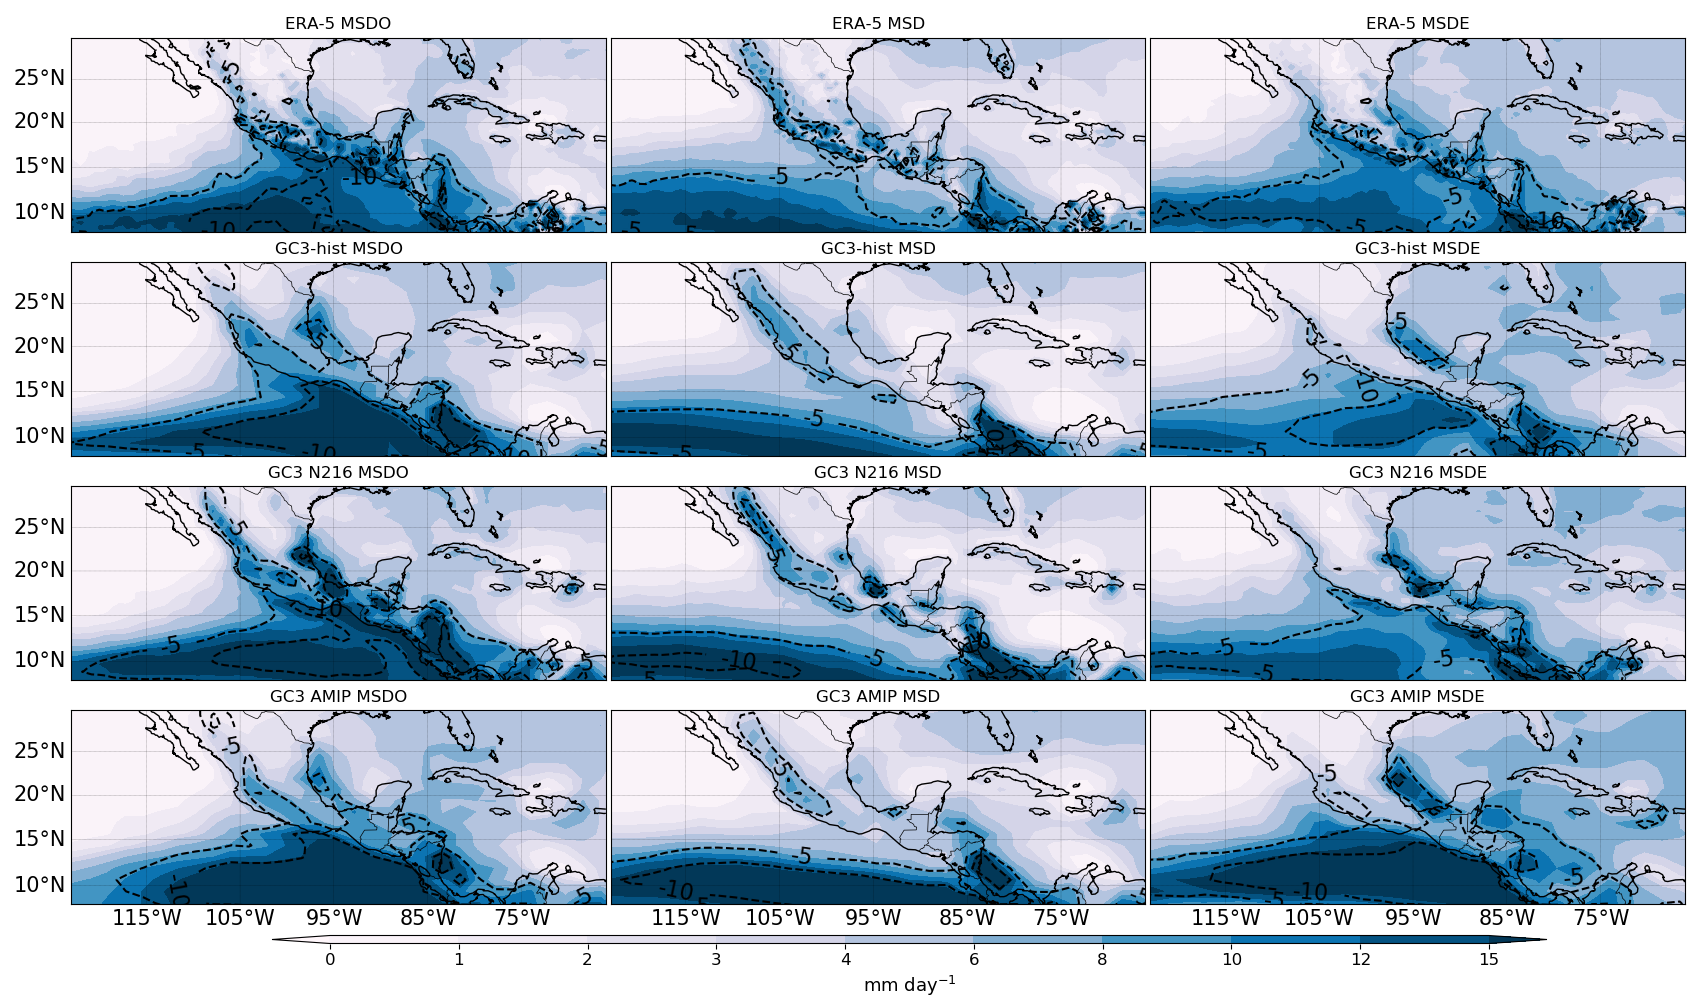
\includegraphics[width=\linewidth]{figures/modcompar_dif2pr3.png}
\caption{Intra-seasonal march (left to right) of precipitation (shaded) and vertical velocity ($\omega$) at 500-hPa in ERA-5, GC3-hist, GC3 N216 and GC3 AMIP (top to bottom). For each dataset, the periods shown are 10 days prior to the onset of the midsummer drought (MSDO), the MSD period and the 10 days after the end of the MSD (MSDE).}
\label{fig:eof2}
\end{figure}


\subsection{ On the mechanisms of the MSD in the UK Met Office models}
\label{sq:chap3}

Biases in the strength and position of the EP ITCZ in Global Coupled Models (GCMs) \citep{bellucci2010,li2014,schneider2014} are a major reason for biases in the model representation of rainfall in Central America  \citep{rauscher2008}. 

\cite{ryu2014} analyzed the performance of CMIP3 and CMIP5 models and found that the majority of CMIP5 models were unable to represent the total annual rainfall and the seasonal cycle of the MSD. \cite{ryu2014} also finds that models that simulate a bimodal distribution of rainfall, HadGEM2-A for example, also show an accurate seasonal cycle of the NASH and the CLLJ. However, an exhaustive analysis as to whether these features are actually driving mechanisms for the MSD in GCMs as in observations is missing from the literature. 


The CMIP6 Met Office models, HadGEM3 and UKESM1, are amongst the first models to simulate a bimodal regime in both Central America and Cuba (Figure \ref{fig:8}a and \ref{fig:msdcaribb}). 
In Central America and southern Mexico, the models simulate a wetter-than-observed first peak of precipitation and a drier MSD period.
% 
The so-called second peak of precipitation found in late August is simulated in close agreement with TRMM, except in the AMIP experiment which has a far too strong second peak mean precipitation rate.
% The seasonal cycle and other characteristics of the MSD showed noticeable differences between the different experiments analysed in this study. 


%\subsubsection{Climatological features of the MSD in UKESM1 and HadGEM3}
%Rainfall during the first peak has been too wet in these models since CMIP3, suggesting a persistent wet bias in this region associated with the East Pacific ITCZ \citep{ryu2014,mulcahy2018}. 
Figure \ref{fig:eof2} shows the distribution of rainfall in the different stages of boreal summer in different CMIP6 experiments and ERA-5. 
The main feature, the East Pacific ITCZ shows the maximum rainfall rates (>15 mm day$^{-1}$ in the models) and strong mid-level ascent (-0.1 Pa s$^{-1}$). Prior to the MSD, rainfall extends from the easternmost Pacific ITCZ into the North American continent. Therefore, the positive bias during the first peak over land is associated with the biased wetter EP ITCZ.  However, during the MSD, rainfall decreases over land remaining only above 10 mm day$^{-1}$ south west of the coastline in the models.



%For example, the Atlantic ITCZ biases have been shown to be directly affected by processes in the convective scheme \citep{bellucci2010}, such as the treatment of entraintment and moisture-cloud feedbacks \citep{oueslati2013,li2014}. 

The wetter EP ITCZ is a common feature of GCMs, including the Met Office models, which results from multiple biases in the radiative and convective schemes \citep{oueslati2013,li2014}. %For instance, the oversensitivity of convection to SSTs in models is a known problem with tropical climate modelling \citep{}.
% The entraintment parameter and cloud-radiative feedbacks have also been shown to play a role in these biases . 
 In UKESM1 and HadGEM3 several biases exist in the radiative balance in the easternmost Pacific Ocean. A positive bias in incoming shortwave in Central America of about 15\% and a cold SST bias in both East Pacific and Caribbean Sea SSTs are observed in Figure \ref{fig:csst}. Increased incoming shortwave but cooler SSTs require increased surface fluxes to maintain energy balance. These higher latent heat fluxes (LHFs) in the models in both basins (Figs. \ref{fig:csst}g, h) are almost 40\% larger than in ERA5 during the first peak of rainfall. The models also exhibit a larger seasonal cycle of the fluxes than the reanalysis. GC3 AMIP is the only simulation to also show a significantly positive bias in LHFs during the second peak of rainfall in the EP but also at the end of MSD in the Caribbean Sea. 


In all the model experiments, the ITCZ prior to the MSD period is stronger than in ERA5 by more than 5 mm day$^{-1}$, whereas after the MSD rainfall in the coupled models on the western coast of Central America agrees well the ERA5. 
This analysis suggests that the biases shown in Figure \ref{fig:7} are mostly coming from the period prior to the MSD. The models reasonably simulate the decrease in rainfall during the MSD (Figure \ref{fig:eof2}) followed by the second increase or peak. 
Note that GC3 AMIP, forced by very similar SSTs as ERA-5, simulated a much larger mean precipitation in the ITCZ during MSDE in contrast to the coupled models. This large positive bias in simulated rainfall in the East Pacific in GC3 AMIP corresponds to the larger than observed second peak observed in Figure \ref{fig:msdcaribb}a. 


 \begin{figure}[t!]
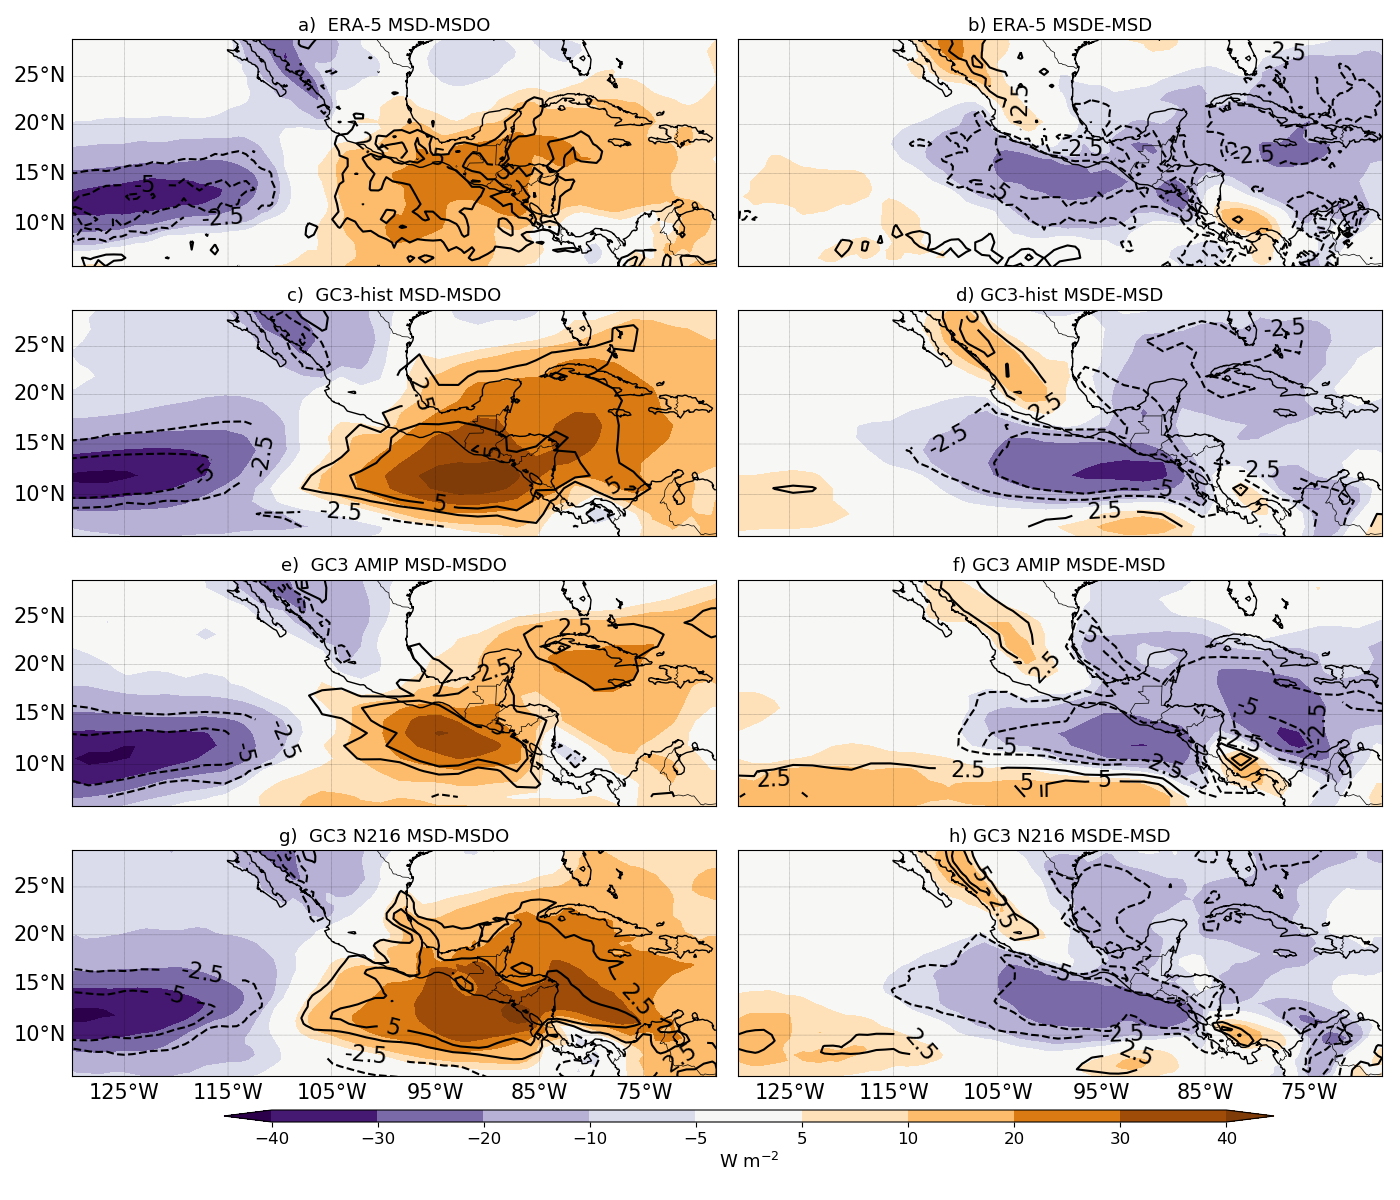
\includegraphics[width=\linewidth]{figures/fig4_olrdiff.png}
\caption{Out-going longwave radiation (OLR) [W m$^{-2}$] (shaded) and $\omega$ 500-hPa [$10^{-2}$ Pa s$^{-1}$] (line contours) differences between the MSD and MSDO and the MSDE and MSD.}
\label{fig:msdolranom}
\end{figure}


 \begin{figure}[t!]
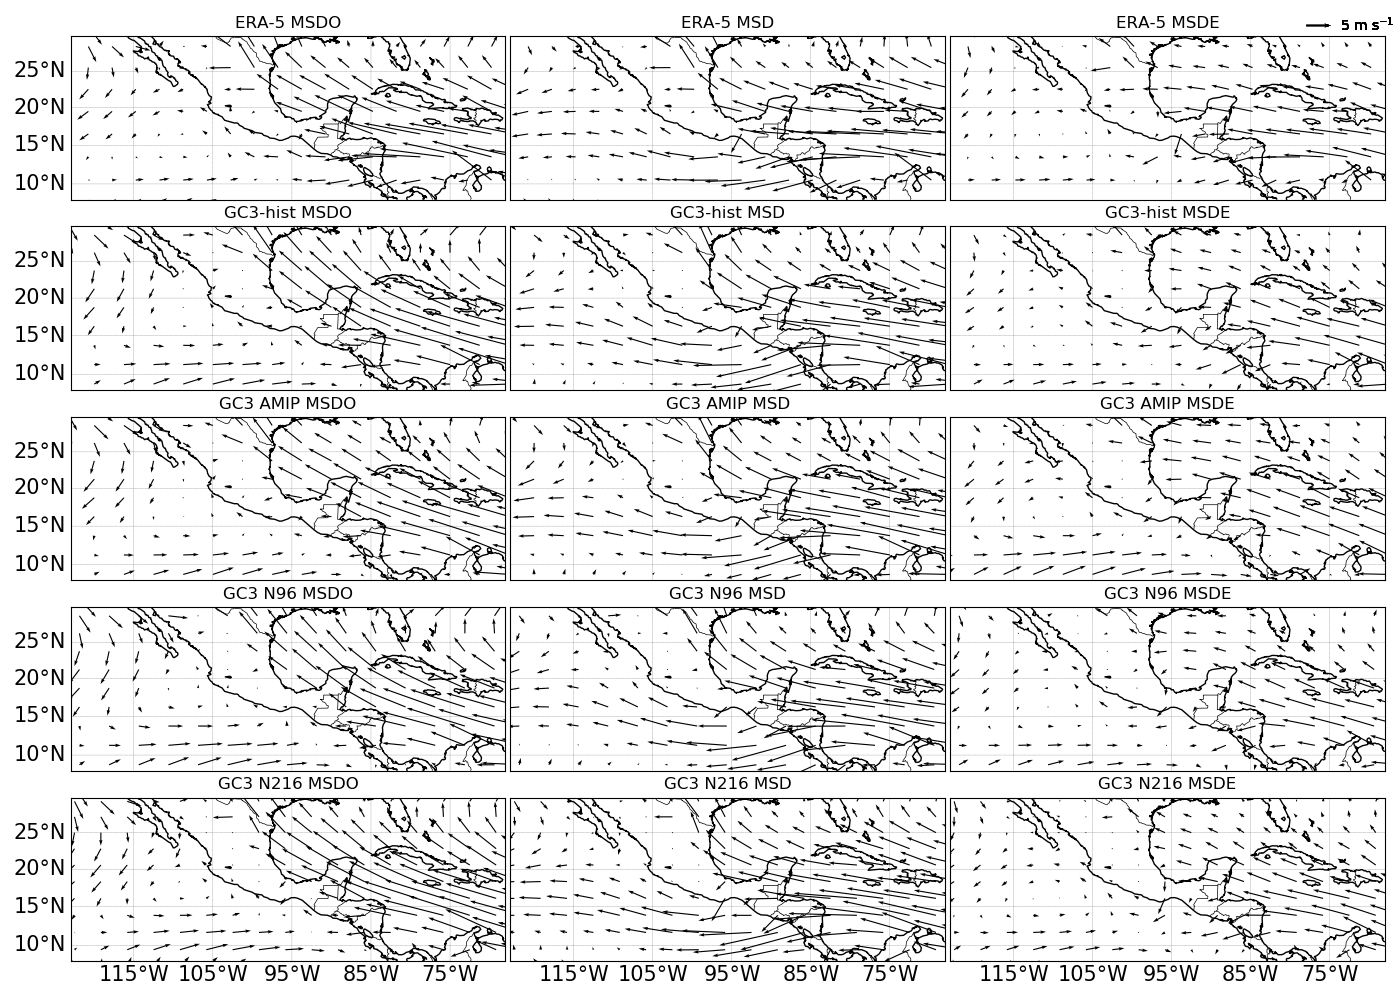
\includegraphics[width=\linewidth]{figures/modcompar_dif2u3}
\caption{As in Figure \ref{fig:msdolranom} but showing wind vectors at the 850 hPa level. }
\label{fig:msduanom}
\end{figure}


Composites prior to the onset of the MSD, during the MSD and after the MSDE were computed for several diagnostic variables. The periods were separated using the WT method to determine the dates of the MSDO and MSDE in ERA5 and the climate model output.
Figure \ref{fig:msdolranom} shows the composite differences between the period of the MSD and of the two peaks in out-going longwave radiation (OLR) and vertical velocity ($\omega-500$) at 500 hPa.
The positive OLR and $\omega$ anomalies in the MSD-MSDO panels in southern Mexico and northern Central America are indicative of decreased height of convection and decreased ascent, in agreement with the MSD being the drier period. These positive anomalies in the continent are accompanied by negative OLR and $\omega-500$ anomalies west of the continent, around 125$^\circ$W. 
%These anomalies are stronger in the simulations (e.g., Figure \ref{fig:msdolranom}c). 


The MSDE-MSD panels show the difference between the second peak of rainfall and the drier MSD period. Negative OLR and $\omega$ anomalies indicate stronger and higher convection over a wide region including the easternmost Pacific Ocean, southern Mexico, northern Central America Cuba and the Caribbean Sea.  
Note also the region of the North American Monsoon, on the northwest corner of Mexico and the southernmost US, as the MSD-MSDO difference suggests increased convective activity in the North American Monsoon region and 
MSDE-MSD the opposite. 

 \begin{figure}[t!]
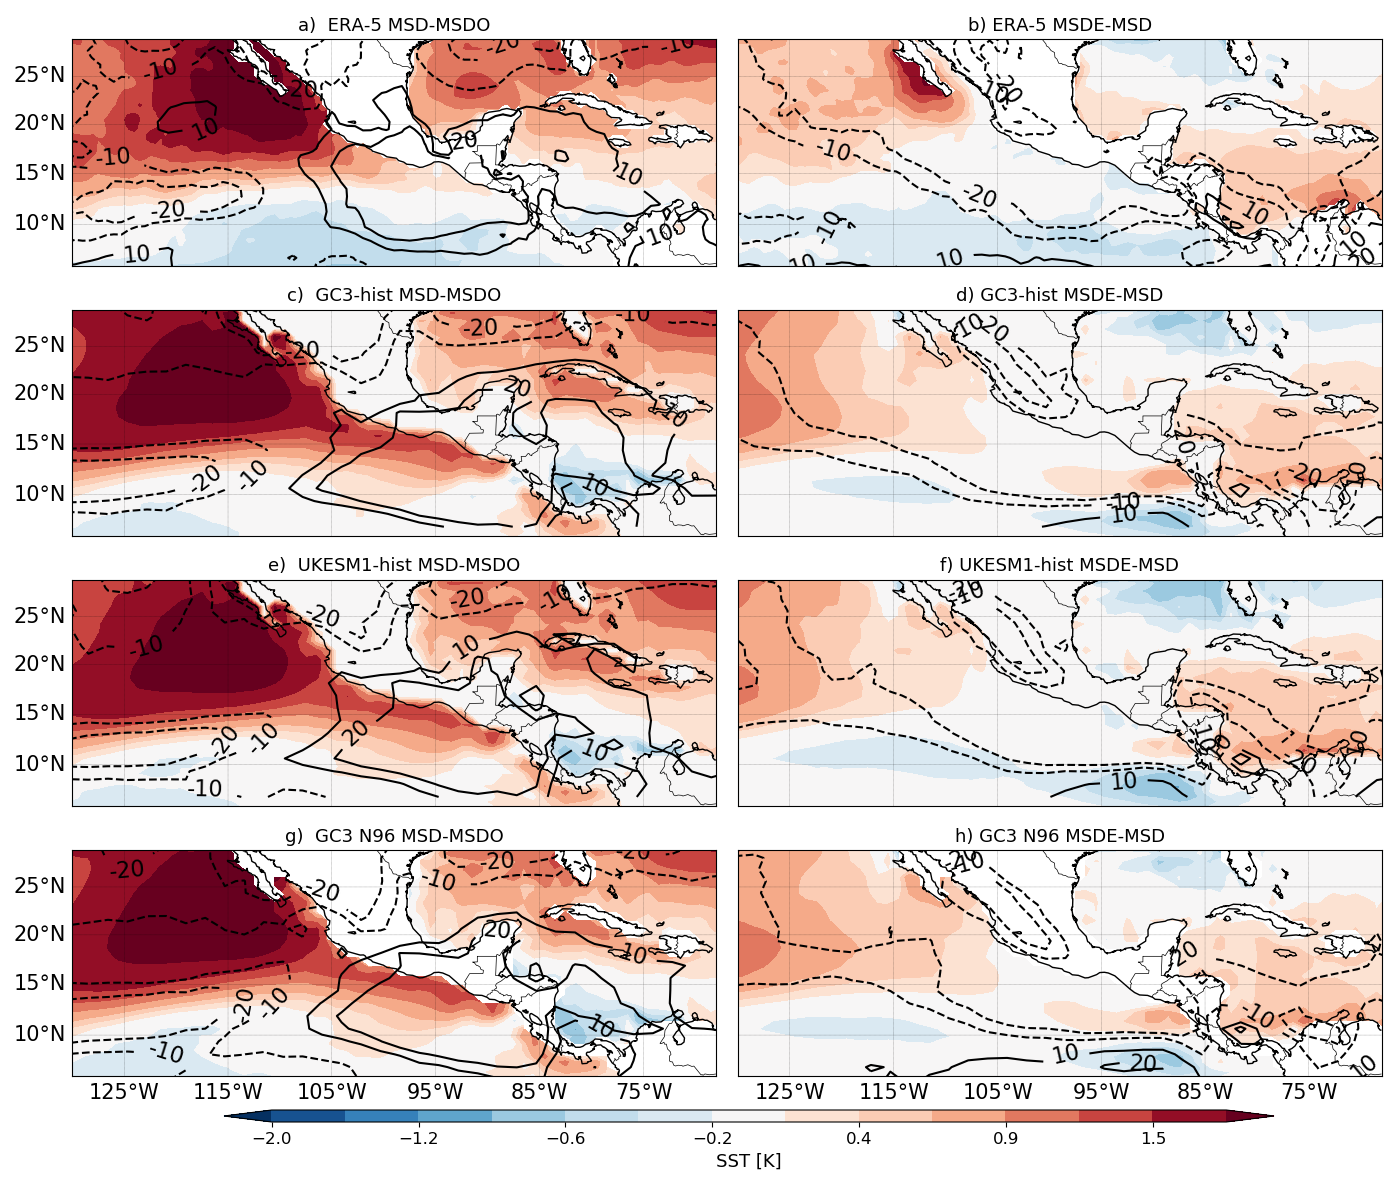
\includegraphics[width=\linewidth]{figures/fig4_sstdiff}
\caption{As in Figure \ref{fig:msdolranom} but the anomalies are shown for SSTs [K] (contours) and incoming shortwave radiation [W m${-2}$] at the surface (line-contours). Incoming shortwave is defined such as negative differences imply less incoming shortave and positive anomalies represent more incoming shortwave at the surface. }
\label{fig:msdsstanom}
\end{figure}

Similarly, Figure \ref{fig:msduanom} shows the low-level wind field during the three stages of the MSD. In ERA-5, prior to the MSD the wind flow in the Caribbean shows strong easterlies that flow into the Gulf of Mexico and southeastern US but very weak winds in the EP (see Figure \ref{fig:csst}f). During the MSD, the winds in the EP become modestly strong eaterlies associated the easterly flow from the Caribbean Sea that crosses over Costa Rica and Nicaragua from the Caribbean Sea to the East Pacific. Note that the easterlies converge towards the region at 125$^\circ$W where OLR and $\omega$ anomalies suggest increased ascent. 

By the end of the MSD the easterlies in ERA5 weaken substantially on the western coast of Central America and in the Caribbean Sea.
The simulations seem to generally reproduce the characteristics of the wind field with some differences worth mentioning. For instance, prior to the onset of the MSD, all the simulations show a modest westerly wind flow in the east Pacific at 10$^\circ$N, which can also be seen in Figure \ref{fig:csst}f, which is not observed in ERA5.
After the MSD ends, most simulations show a very weak westerly flow in the East Pacific, close to ERA5; however, GC3 AMIP shows a modest westerly wind converging towards the west coast of Nicaragua. This low-level convergence may be forcing the increased convective activity and precipitation during this time in GC3 AMIP.

The SSTs and incoming shortwave radiation are key elements for explain the seasonal cycle of the MSD, according to previous theories summarised in section \ref{sq:lit}. 
Figure \ref{fig:msdsstanom} shows the corresponding SST and incoming shortwave anomalies during the different stages of the seasonal cycle. % MSD-MSDO and MSDE-MSD anomalies. 
From the first peak to the MSD, a positive SST difference of +1.5 K in the Gulf of California and the western coast of the Baja California Peninsula is observed in reanalysis and the models. The differences appear as a sharp SST meridional gradient pattern around 115$^\circ$W. 
During this stage, the incoming shortwave increases in Central America, which agrees with Figure \ref{fig:csst}d. 
Note the negative incoming shortwave differences west of Central America at 125$^\circ$W, the region of negative OLR and $\omega$-500 hPa anomalies where low-level winds converge, all of which supports the notion of increased convective activity that reduces incoming shortwave west of the continent. This feature was noted by \cite{herrera2015}. 

 \begin{figure}[t!]
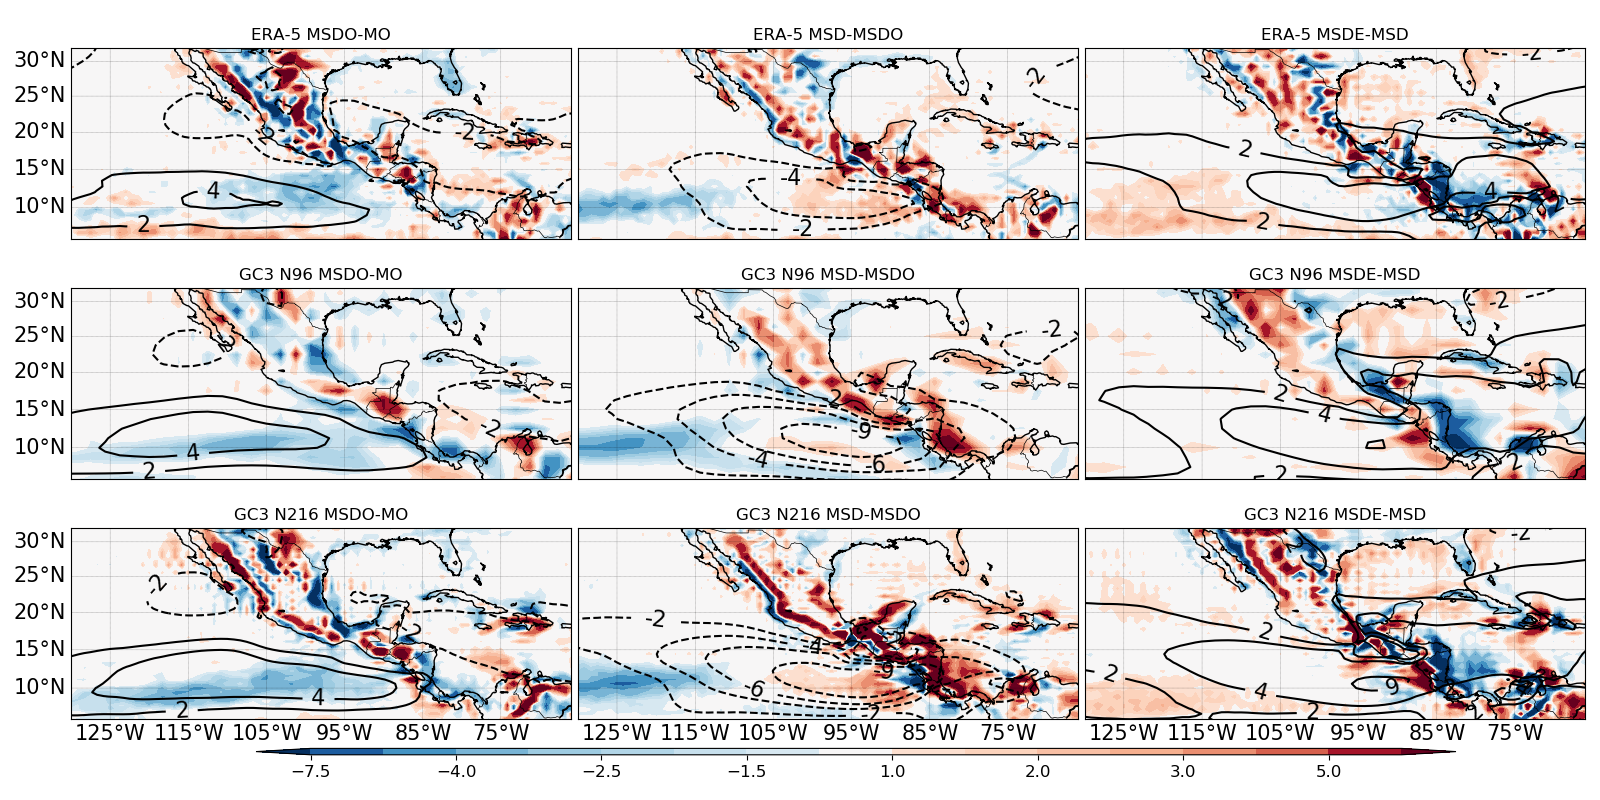
\includegraphics[width=\linewidth]{figures/modcompar_dif2mfc3}
\caption{As in Figure \ref{fig:msdolranom} but showing in shading, moisture flux divergence $\nabla \cdot \vec{u}q$ at the 850 hPa level with units of $10^{-7}$ s$^{-1}$ kg / kg and zonal wind anomalies (line contours) in m s$^{-1}$.  }
\label{fig:msdmfcanom}
\end{figure}

After the MSD, the western coast of the Baja California Peninsula continues to warm and the East Pacific continues to cool, in contrast to previous suggestions \citep{magana1999,magana2005,herrera2015}. Meanwhile, the Caribbean Sea warms by 1 K and the northern Gulf of Mexico slightly cools down. The incoming shortwave differences show a regional-scale decrease in incoming shortwave, as the summer draws to an end. 
These SST differences indicate that the meridional SST gradient in both the EP and Caribbean Sea and Gulf of Mexico is greatly modified during the stages of the MSD. 


The main dynamical argument put forth to explain the MSD is centred around variations in the moisture flux convergence (MFC), argued to be driven by the Caribbean-Low Level Jet \citep[see e.g.][]{gamble2008,herrera2015,martinez2019}. The MFC and zonal wind variations in each stage of the MSD is shown in Figure \ref{fig:msdmfcanom} for ERA-5 and two simulations. The low-level MFC increases from monsoon onset (MO) to the first peak period (MSDO) in the EP. This anomaly in MFC corresponds to a region of positive zonal wind anomalies indicative of weaker easterly flow.
 This zonal wind anomaly from MSD to MSDO is much stronger in the models.  
The MSD-MSDO difference shows a strong positive MFC anomaly across southern Mexico and most of Central America. 

In turn, the MFC anomalies associated with the end of the drier period, observed as the MSDE-MSD anomalies,  show negative values, suggesting increased moisture flux, over southern Mexico and northern Central America.
Increased moisture flux during the transition from the MSD to the second peak agrees well with the precipitation differences during these periods.  The MSDE-MSD zonal wind anomalies in the EP show positive zonal wind anomalies, suggesting a weakened easterly wind flow (see also Fig. \ref{fig:msduanom}). 

The MSD in Central America and southern Mexico has been strongly linked to the strengthening of the CLLJ \citep{herrera2015}. The maximum zonal wind observed in the CLLJ is found at the very end of July (Fig. \ref{fig:csst}e), synchronized with the start of the MSD. 
The zonal wind anomalies in the MSD-MSDO panels in Figure \ref{fig:msdmfcanom} show that easterlies in the Caribbean Sea do not strengthen by more than 2 m s$^{-1}$ from the first peak to the MSD. Only in the models is there a modest negative anomaly at the westernmost Caribbean Sea. In other words, while the peak of the climatological CLLJ coincides with the climatological timing of the onset of the MSD, these composite analyses constructed by more specifically separating the MSD periods does not show relevant variations in the zonal wind of the Caribbean Sea. 
The drier MSD period does coincide with stronger easterly flow over the eastern Pacific, which may be associated with the weaker MFC over land. %The end of the MSD then coincides when the easterly winds weaken. 

\subsection{Summary and discussion}\label{sq:sumdiscuss}


 \begin{figure}[t!]
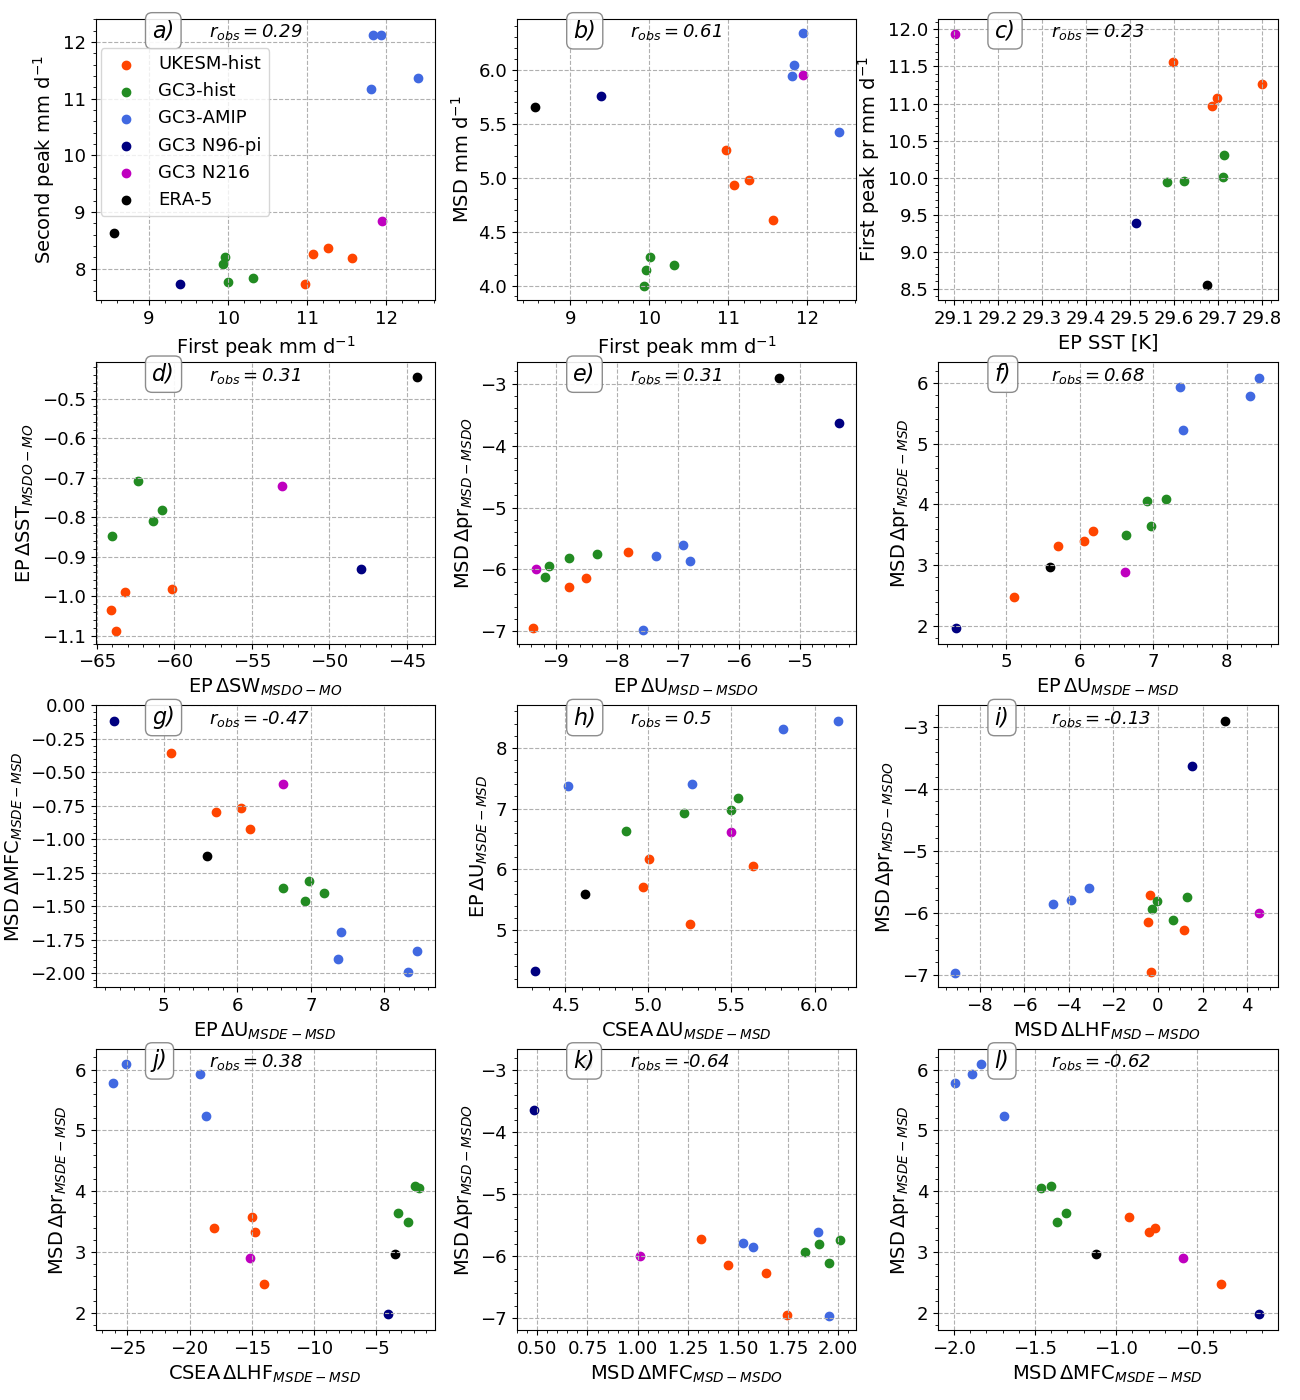
\includegraphics[width=\linewidth]{figures/scatter}
\caption{Scatter plot of the (a, b) area-averaged precipitation over land  (Box in Figure \ref{fig:7}) during the different stages of the MSD. (c) scatter of the East Pacific SSTs against  the precipitation over landduring the first peak period. (d-l) show the scatter differences in several variables between the different stages of onset of the MSD (MSDO), the drier MSD and the end of the MSDE. The differences are shown for area-averaged quantities in the East Pacific (EP), the Caribbean Sea (CSEA) and overland (MSD) as above. The units for $\Delta$U are [m s$^{-1}$], $\Delta$MFC [10$^{-11}$ s$^{-1}$], $\Delta$SW and $\Delta$LHF [W m$^{-2}$] and $\Delta$pr mm d$^{-1}$.   The Pearson correlation coefficient for the 38 yr of  reanalysis or observations ($r_{obs}$) is shown for each panel. }
\label{fig:scatter}
\end{figure}

The midsummer drought  is a  prominent feature of the seasonal cycle of rainfall of southern Mexico, northern Central America and the Caribbean. The average 20\%  decrease during the midsummer compared to the wetter periods of early and late summer is a rare feature of monsoon regions that has important implications for agriculture and water management  \citep{hellin2017,de2018,harvey2018}. 

Climate predictions of the MSD, particularly those concerning whether this "drought" will become more pronounced in the following years, are not trustworthy because of several reasons. 
One factor is the current limitation in the understanding of the physical processes that cause the MSD (section \ref{sq:lit}) as debate still exists over which large or regional-scale processes are most important to explain the increases and decreases of precipitation over intraseasonal time-scales.
Secondly, methods used to diagnose the timing and strength of the MSD typically deal with monthly-scale metrics, which would obscure subtle trends and processes that have an effect on shorter time-scales. 
Also relevant is the fact that climate models used to produce the predictions show significant biases in the EP ITCZ and the seasonal cycle of rainfall in the region, in fact, most CMIP3 and CMIP5 models did not show a bimodal signature in the seasonal cycle. Models that do not have a climatological MSD cannot provide a prediction for this regime in future climate. 

For these reasons, this section analysed the CMIP6 simulations from the Met Office models, UKESM1 and HadGEM3, aiming to understand the causes of the biases in the seasonal cycle. Furthermore, these models are better compared to CMIP3 and CMIP5 cohorts since UKESM1 and HadGEM3 actually simulate a bimodal precipitation regime in these regions. 
The purpose of this investigation is to use these climate models to better diagnose the relevant biases for the representation of the MSD but also understand the processes that these models are capturing leading to the MSD, in order to, hopefully, also highlight the dynamics of the MSD in general. 
%Therefore,this section and future thesis chapter evaluates the similarities and differences between reanalysis and model experiments. 
% For varios reasons, determining the timing and strength of the MSD is very important to agricultural practices,  and water management planning. 





%The different experiments showed notable differences in the precipitation amount in the MSD seasonal cycle.  The first peak, however, appears to be modestly related  to the precipitation amount during the MSD in the models and in observations ($r=0.6$) suggesting that the wetter the first peak the wetter the MSD period.  


 The wavelet transform method was developed to determine the pentads of onset and end of the MSD.  For instance, Figures \ref{fig:scatter}a,b show the scatter of the mean precipitation during the first peak against second peak and first peak against MSD in all the simulations and ERA5. The magnitude of the first and second peaks appear to be unrelated in these models and in observations, which would suggest that the processes driving each peak are not exactly the same.
 Similarly, composite analysis of various diagnostics during the different stages of the seasonal cycle was done, for instance,  OLR composites showed that the MSD is not a local feature in a small region of southern Mexico but extends throughout a wide range of North America,  from central Mexico through Belize, Guatemala, El Salvador, Honduras, Nicaragua, and northern Costa Rica. % Although the MSD has been documented in all these regions \citep{magana1999,perdigon2018}, these composites showed a synchronicity in the precipitation anomalies and a larger extent to the western Mexican coastline that were not previously shown, to our knowledge. OLR anomalies between the second peak and the MSD also showed a simultaneous increased convective activity in the Caribbean. 
 
 This composite approach also allowed to test previously proposed hypotheses by analysing the differences between model experiments and the observed variability in the characteristics of the precipitation at each stage of the MSD.
 For example, \cite{magana1999} proposed a mechanism that explains the MSD through SST-cloud feedbacks. In this hypothesis, shortwave, SSTs and precipitation are strongly coupled in the EP Ocean. The first peak of precipitation in southern Mexico and Central America would then be associated with the EP SSTs prior to the onset of rainfall. 
 Figure \ref{fig:scatter}c shows that EP SSTs prior to onset do not explain the inter-model differences in the magnitude of the first peak nor do they show a strong relationship in the observed interannual variability of the first peak mean precipitation. 
 Similarly, Figure \ref{fig:scatter}d shows that surface incoming shortwave variations are only weakly related to SSTs variations in the EP, in both models and reanalysis, during the first peak period. 
 
The feedback mechanism also suggests that the second peak is a result of a second increase in surface incoming shortwave that occurs as cloud cover decreases during the drier MSD. This increase in incoming shortwave then increases EP SSTs and thus increasing convective activity. Although the incoming shortwave does show a bimodal behaviour (Figure \ref{fig:csst}d), the SSTs in the East Pacific do not increase during the MSD period, but in fact cool during the end of the MSD.   Furthermore, as in Figure \ref{fig:scatter}d, variations in incoming shortwave were not strongly related to SST changes in any of the stages of the MSD (not shown). This suggests that the SSTs are not only dependent on the incoming shortwave in both models and reanalysis.

The low-level winds (Figure \ref{fig:msduanom}) show notable changes between the onset of the MSD (MSDO), the MSD and the end of the MSD (MSDE).
  Weak westerlies in the EP are found during the wetter periods but the zonal wind becomes a modest easterly flow during the drier MSD period. 
  The MSDO appears to be synchronized with the strengthening of the Caribbean Low-Level Jet (Fig. \ref{fig:csst}e). During the MSD, the strong zonal flow in the Caribbean crosses Central America into the central-eastern Pacific. This easterly flow during the MSD converges to 125$^\circ$W in the EP Ocean, a region that also shows increased ascent during the MSD. 
 % The zonal wind the East Pacific seems to be modulated by the wind in the Caribbean Sea, i.e., by the Caribbean Low-Level Jet strength.
 
Figure \ref{fig:scatter}e, f show the relationships between the zonal flow in the EP Ocean and precipitation in southern Mexico and Central America. 
The changes in the wind flow between the first and the MSD are not related to the drying response over land during the same period. 
However, the differences between the second peak and the MSD in the wind flow and precipitation show a strong relationship both in observed interannual variability as well as in the model spread. Simulations with a stronger EP zonal wind anomaly show the strongest increment in precipitation over land.
The zonal wind change in the EP from the MSD to the second peak period is also modestly related to the MFC over the continent (Fig. \ref{fig:scatter}g) with weaker easterly winds in the EP associated with more convergence over land in the models and reanalysis. 


%is associated with the variability observed in the precipitation changes from the MSD to the second peak, as well as with the MFC in the MSD region.  
The easterly flow in the EP has been associated with the strength of the CLLJ \citep{herrera2015}. The zonal wind changes in the MSDE-MSD difference in the EP shows a modest linear relationship with the zonal flow in the Caribbean Sea (Fig. \ref{fig:scatter}h). During the other periods, the relationship between the CLLJ and the EP zonal component of the wind is even weaker in both models and observations (not shown). 

%However, the zonal wind in the Caribbean Sea is not linearly related to MFC in the MSD region (panel g). In other words, it appears the CLLJ influences the EP zonal flow but not the MFC or precipitation in the MSD directly. 
 
A potentially relevant bias found in the models was stronger-than-observed surface latent heat fluxes (LHF) (Figure \ref{fig:csst}g, h) compared to the reanalysis.  Changes in the surface energy balance and the surface temperature in historical versus pre industrial control simulations may also be responsible for the precipitation differences between these experiments.  However, the variations in the LHFs, both MSD-MSDO and MSDE-MSD either in the Caribbean Sea or over land (Figure \ref{fig:scatter}i,j) are not related to precipitation over land.



The main factor associated with the precipitation variations in the seasonal cycle appears to be the low-level moisture flux convergence (MFC) (Figure \ref{fig:scatter}k, l). The variations in the MFC over land explain intermodel differences and observed interannual variability in precipitation, particularly in the positive rainfall increment from the MSD to the second peak. From the first peak to the MSD, moisture flux decreases and increases again from the MSD to the second peak. % The lowest decrease Stronger moisture flux into region leads to   
 

\chapter{\label{ch:7-qbo} The tropical route of QBO teleconnections in UKESM1 and HadGEM3 }

Evidence in a previous chapter suggests that the QBO plays a role in tropical ENSO teleconnections associated with the Walker circulation in the CMIP6 experiments of the MOHC models.
In this chapter, the influence of the QBO on the tropical mean circulation and teleconnections is more closely examined in these models. An analysis of the CMIP6 experiments from the MOHC shows  how the tropical circulation, monsoons and the ITCZ are influenced by the QBO. Results are discussed in the context of existing observational evidence of QBO tropical teleconnections. 

%Secondly,  numerical experiments with the MOHC models were designed and performed to test the hypothesis thata relaxation of the zonal wind the equatorial stratosphere towards a reanalysis dataset are described and compared with free-running simulations.

\section{Introduction}

Long-distance effects or teleconnections associated with the stratospheric quasi-biennial oscillation (QBO) have been well documented in the subtropics and extratropics, for example for the stratospheric polar vortex \citep{holton1980,anstey2014,lu2020}, the subtropical jets \citep{garfinkel2011,hansen2016tropospheric} and the North Atlantic Oscillation \citep{hansen2016tropospheric,gray2018,andrews2019observed}.  
 Observational and modelling evidence suggests that there is also a tropical route of influence of the QBO to surface climate, for example, over tropical convective phenomena such as monsoons \citep{giorgetta1999,liess2012}, the ITCZ \citep{gray2018}, tropical cyclones \citep{gray1984,chan1995} and most recently, the Madden-Julian Oscillation (MJO) \citep{lee2018,wang2019,martin2020jgr}, see section \ref{sq:trop_qbo}. 
 
Several observational and modelling studies have found evidence of QBO-related influence over convective activity in monsoon regions, such as in the South American, East Asian, Australian and Indian monsoons \citep{giorgetta1999,collimore2003,liess2012,gray2018}. 
In observations, these responses have been found in satellite-derived fields such as cloud height, occurrence and out-going longwave radiation \citep{collimore2003,liess2012}, as well as in surface precipitation diagnosed from gridded datasets or from reanalysis \citep{gray2018}.
However,  the observational evidence shows zonally asymmetric impacts, indicative that the impact of the QBO depends on longitude, which has been explained \citep[e.g. by][]{collimore2003,liess2012} through a QBO modulation of the Walker circulation.

In models,  \cite{giorgetta1999} finds that boreal summer monsoon regions exhibit a significant response in cloudiness to QBO winds within the GCM ECHAM4. 
\cite{nie2015} further finds in a modelling framework that the influence of the QBO may depend on the strength of convection and SST forcing, suggesting a non-linear effect of the QBO over a convective profile. In CMIP5/CMIP6 models, only a relatively small number of studies have analysed tropical QBO teleconnections \citep{serva2021}, as most studies focus on the polar and subtropical routes \citep{richter2020,anstey2021}. 

 Although the polar and subtropical routes of influence of the QBO to the surface are relatively well established, the impact of the QBO over tropical convective phenomena remains less well understood for various reasons. First, the short observational record limits the confidence in any analysis that seeks to investigate differences between the two QBO phases in a 30-40-yr long dataset. Tropical circulation variability on QBO time-scales is largely dominated by ENSO, which makes it difficult to separate the effects of ENSO and the QBO, other than by multi-variable regression analysis as in \cite{gray2018}. In addition, there is also evidence that ENSO and convection in the Pacific influence the QBO, so there is a two-way relationship that would difficult a separation of cause and effect \citep{schirber2015,christiansen2016}. 
 
 
In addition, the specific physical mechanisms through which the QBO could influence tropical convection at the grid-scale or the large-scale tropical circulation are also not well understood. 
While early studies \citep{gray1984,collimore2003} suggest that changes to the vertical wind shear or static stability in the upper-troposphere lower-stratosphere (UTLS) region are the cause of these teleconnections, there is a lack of evidence in the literature to support any mechanism over another. 
As such, studies have struggled to pin-point direct impacts and mechanisms by which the QBO may modulate any aspect of tropical climate. 

This chapter investigates QBO tropical teleconnections in the pre-industrial control experiments of the MOHC UM: GC3 N96-pi, GC3 N216-pi, UKESM-pi. These simulations are ideal to investigate variability associated with the QBO because these experiments are very long integrations where external forcing is kept constant within the simulation and the UM is a model that reasonably simulates the QBO \citep{richter2020}. 
The remainder of this chapter is presented as follows. 
First, the data and methods used are described, after which the results analysing the QBO impacts over the seasonal precipitation and surface temperatures  is given. 
Then, a more detail investigation on the effects on the East Pacific and Atlantic ITCZs is presented and finally, the impacts over ENSO, the Indian Ocean and the Walker circulation are given. 
A discussion is given at the end of the chapter.
% These simulations are examined first via composite analysis to investigate whether tropical convective phenomena such as the ITCZ and monsoon rainfall show any significant response to the state of the QBO. 





\section{Methods and data}

The observational datasets and reanalysis (ERA5) used in this chapter are described in section \ref{sq:obsdata} and consist of the HadSST3 dataset for SST, GPCP for precipitation and ERA5 for the rest of the diagnostics that include the zonal and meridional winds, air temperature, etc.

\subsection{CMIP6 data}

The three pre-industrial control experiments of the MOHC submitted to CMIP6 are used in this chapter: GC3 N96-pi, GC3 N216-pi and UKESM-pi. UKESM-pi and GC3 N96-pi are run with the same resolution (N96) of 1.875$^\circ$x1.25$^\circ$ and GC3 N216-pi is considered a medium-resolution simulation (N216) with atmospheric resolution of 0.83$^\circ$x 0.56$^\circ$. The period of 1850-2350 is used for GC3 N96-pi and GC3 N216-pi and 2050-2650 for the UKESM-pi. 


\subsection{Indices}

The indices for ENSO and the QBO are diagnosed exactly as in section \ref{sq:meth_ch4}, i.e., the 70-hPa zonal mean zonal wind index is used for the QBO with a threshold of 2 m s$^{-1}$ for each phase and the EN3.4 index is used with a threshold of $\pm$0.65 to define positive or negative events.

\subsection{Analysis techniques}

Composite analysis is the preferred technique used throughout this chapter. For each QBO or ENSO phase, composite samples are drawn for specific seasons using the indices and definitions mentioned above. 
Statistical significance is estimated in various ways, in some cases through standard Student or Welch t-test's where specified, and in some other cases a randomised resampling or bootstrapping method is also implemented in several sections of the chapter. 
The bootstrapping method is performed in all cases by drawing random samples from the entire simulation and repeating the process 10,000 times to evaluate the likelihood of obtaining a relationship by chance. 

Linear regression analysis has proven useful to understand the effect of one or more aspects of the climate over a region or a time-series, and was used to investigate the surface impacts of the QBO in observations by \cite{gray2018}. 
A simple linear regression model can be written as:

\begin{equation}
Y(t)=X_0+X_i(t)\beta_i + \epsilon,
\end{equation}
\noindent where $Y$ is the measured or dependent variable, $X_0$ is a constant coefficient, $\beta_i$ is the regression coefficient between $X_i$ and $Y$ and $\epsilon$ represents random error or a residual. 
A multivariate regression model can be used to study the joint effect of two or more predictors over a variable ($Y$) such that the model can be written as:
\begin{equation}
Y(t)=X_0+\sum_j^NX_j(t)\beta_j+\epsilon
\end{equation}
\noindent where $X_j(t)$ is any predictor with an associated regression coefficient $\beta_j$. 
As in previous studies \citep{gray2018,misios2019slowdown}, the regression coefficient can be rescaled to evaluate the total effect that a predictor ($X_j$) can have on the variance of the measured variable ($Y$) using the standard deviation ($\sigma_j$) and the maximum ($X_{j,max}$) and minimum ($X_{j_min}$) values of $X_j$ so that the rescaled coefficient $\beta_j^\prime$ can be written as:

\begin{equation}
\beta_j^\prime=\beta_j\frac{X_{j,max}-X_{j,min}}{\sigma_j}.
\end{equation}
\section{Teleconnections in the pre-industrial control experiments}\label{sq:cmip6_qbo}

\begin{figure}[b!]
\centering
 %\noindent
 \includegraphics[width=\linewidth]{figures/piprclimqbowqboe.png}
\caption[Annual mean precipitation composite difference QBO W-E ]{ Annual mean precipitation difference between QBO W-E phases in (a) GPCP, (b) GC3 N96-pi, (c) GC3 N216-pi and (d) UKESM-pi. Hatching denotes statistical significance to the 95\% confidence level using bootstrapping with replacement for each composite sample. }
\label{fig:qboclim}
\end{figure}

Surface impacts of the QBO in the tropics have scarcely been investigated in CMIP models, as most studies focus on the general representation of the QBO \citep[e.g][]{schenzinger2017,bushell2020}, or the extratropical teleconnections \citep[e.g.][]{anstey2021,dimdore2021}. 
However, studies that have investigated teleconnections between the QBO and tropical convective phenomena in relatively novel GCMs \citep[e.g.][]{lee2018,martin2021,serva2021} have found that model biases in representing the variability of temperature and winds in the tropopause layer may hinder a possible interaction between the QBO and tropical convection. 

This section examines more closely how the MOHC piControl experiments simulate the effect of the QBO over seasonal-mean precipitation, monsoons and the ITCZ. 
The three simulations chosen use the same model setup, with constant year 1850 forcing, but differ in their horizontal resolution or the treatment of aerosol-chemistry processes (see section \ref{sq:modeldata}). 


\subsection{Seasonal variability}

\begin{figure}[t!]
\centering
 %\noindent
 \includegraphics[width=\linewidth]{figures/piprdjfqbowqboe.png}
\caption[DJF mean precipitation composite difference QBO W-E ]{ As in Figure \ref{fig:qboclim} but for DJF. }
\label{fig:qbodjf}
\end{figure}

The composite difference in annual mean precipitation between QBO W and E phases (Figure \ref{fig:qboclim}) shows that in observations (GPCP) the tropical Pacific, equatorial Atlantic and the Indian Oceans are the regions of possibly largest influence of the QBO, which agrees with previous studies \citep{liess2012,gray2018}. The three GCM simulations agree well with the pattern in GPCP, as all three simulations show a positive difference (QBO W-E) in the Central Pacific and the Indian Ocean, albeit the differences are smaller in the simulations. However, the patterns and magnitudes of the impacts become larger when analysed over specific seasons. %, and in fact, the pattern exhibits strong seasonal variability. 

\begin{figure}[t!]
\centering
 %\noindent
 \includegraphics[width=\linewidth]{figures/piprmamqbowqboe.png}
\caption[MAM mean precipitation composite difference QBO W-E ]{ As in Figure \ref{fig:qboclim} but for MAM. }
\label{fig:qbomam}
\end{figure}

For example, during DJF (Figure \ref{fig:qbodjf}), the pattern over the Central Pacific is stronger in GPCP and the simulations relative to the annual mean difference. The positive difference in the western Indian Ocean and the South Pacific Convergence Zone is also observed in this season and is significant in all the datasets. Results in GC3 N216-pi suggest a weakening of the Atlantic ITCZ as in GPCP, whereas UKESM-pi and GC3 N96-pi show little and not significant responses in that region.
The response in the East Pacific during DJF matches the results of \cite{serva2021}, and suggests a southward shift of the ITCZ.
%had been previously 


Similarly, during MAM (Figure \ref{fig:qbomam}), the strongest response arises in the East Pacific and Atlantic ITCZ regions. In GC3 N216-pi the East Pacific ITCZ is shifted southwards whereas in the Atlantic the ITCZ is displaced northward. UKESM-pi agrees with the northward shift of the Atlantic ITCZ and suggests a wetter northern South America during QBO W than E. In GC3 N96-pi, the differences are smaller and the most noteworthy pattern is found in the Western Pacific. 
%Although the impact of the QBO over the ITCZ position has been previously described \citep{gray2018,serva2021}, less is known about the specific mechanisms leading to the change in position and strength of the ITCZ. 


\begin{figure}[t!]
\centering
 %\noindent
 \includegraphics[width=\linewidth]{figures/piprsonqbowqboe.png}
\caption[SON mean precipitation composite difference QBO W-E ]{ As in Figure \ref{fig:qboclim} but for SON. }
\label{fig:qboson}
\end{figure}


In boreal fall (Figure \ref{fig:qboson}), all datasets show relatively large and significant differences in the Indian Ocean, characterized by a dipole of wet anomalies to the west and dry anomalies to the east. These dipole anomalies may be an indication that the QBO influences the Indian Ocean Dipole (IOD), characterized by a zonal gradient of SSTs in the Indian Ocean. In addition, results for GC3 N96-pi and GC3 N216-pi suggest a similar response in the Central and Eastern Pacific as in the other seasons, characterized by a wet anomaly at about 10$^\circ$N.

Finally, the JJA seasonal mean pattern (Figure \ref{fig:qbojja}) shows a weak response in GPCP whereas the simulations show a number of significant differences. Specifically, the three experiments suggest a wet anomaly in the Caribbean Sea and the Indian Ocean; the former, likely related to the northward shift of the Atlantic ITCZ observed in the same season particularly in UKESM-pi. West of the Caribbean Sea, in the easternmost Pacific Ocean a seemingly southward shift of the ITCZ is observed with a negative precipitation response on the western coast of Mexico.
A wetter Indian Ocean is observed in all the simulations and in UKESM-pi the wet anomaly extends over land into the Indian monsoon region.

\begin{figure}[t!]
\centering
 %\noindent
 \includegraphics[width=\linewidth]{figures/piprjjaqbowqboe.png}
\caption[JJA mean precipitation composite difference QBO W-E ]{ As in Figure \ref{fig:qboclim} but for JJA. }
\label{fig:qbojja}
\end{figure}


 Note that in the annual and seasonal mean patterns there little or no differences over land in most seasons, however, two exceptions are observed in Figure \ref{fig:qbojja}. 
A positive and significant response over land is observed in southern Mexico and Central America in all three simulations. Another positive and significant response is observed over the Indian monsoon region, although this signal is only present in UKESM-pi. 

\begin{figure}[t!]
\centering
 %\noindent
 \includegraphics[width=\linewidth]{figures/pisstclimqbowqboe.png}
\caption[Annual mean SST difference QBO W-E under different QBO phases.]{ As in Figure \ref{fig:qboclim} but for SSTs.}
\label{fig:sstclim}
\end{figure}

The simulated and observed precipitation responses in the Central Pacific resemble an El Niño pattern, especially during DJF. In observations, this pattern is likely a result of the increased frequency of El Niño events for QBOW than in QBOE \citep{liess2012}. 
For this reason, similar differences are obtained for SSTs (Figure \ref{fig:sstclim}) which show that the QBO W-E SST appear as an El Niño pattern characterized by increased SSTs over the Central and Eastern Pacific, extending to the equatorial Atlantic. 
Although these differences are much weaker than the signal for a typical El Niño event, these differences are significant in all the simulations.% as well as in the HadSST dataset. 

\begin{figure}[t!]
\centering
 %\noindent
 \includegraphics[width=\linewidth]{figures/pisstdjfqbowqboe.png}
\caption[DJF mean SST difference QBO W-E under different QBO phases.]{ As in Figure \ref{fig:sstclim} but for DJF.}
\label{fig:djfclim}
\end{figure}

The specific SST pattern for DJF confirms that the SST pattern seen in the annual mean difference is stronger during the boreal winter season, particularly for GC3 N96-pi and for the HadSST dataset. The significant responses in GC3 N96-pi over the North Atlantic and in the Indian Ocean also agree very well with HadSST. Results in GC3 N216-pi and UKESM-pi also show a positive SST difference over the Central Pacific during DJF although not significant. 
In the case of GC3 N216-pi the strongest SST anomalies over the Central Pacific appear during MAM (not shown) whereas for UKESM-pi the pattern appears during La Niña events with litte-to-no response during other phases of ENSO (not shown).  

In summary, this section presented the seasonal mean response in precipitation to the phases of the QBO. The main responses in the models were the ITCZ shifts over the Pacific and Atlantic Oceans, but robust signals also suggest wetter conditions in the Indian Ocean and the Caribbean Sea during QBOW compared to QBOE. The results in this section suggest a strong variation of the response with the seasons and with ENSO phase and little overall effect over land regions.
For this reason, the following two sections more closely examine the effect of the QBO over the ITCZs in the East Pacific and Atlantic ITCZs, the Indian Ocean Dipole (IOD) and land-averaged precipitation over monsoon regions. 

\subsection{Impacts over the ITCZ and the monsoons}

\begin{figure}[t!]
\centering
 %\noindent
 \includegraphics[width=\linewidth]{figures/climcmip_bconv_pratl.png}
\caption[ITCZ seasonal cycle in the Atlantic Sector.]{(a) Monthly and zonal-mean convective precipitation in ERA5 in the Atlantic sector [60$^\circ$W-20$^\circ$W. (b-d) Biases in GC3 N96-pi, GC3 N216-pi and UKESM-pi. }
\label{fig:itczclimatl}
\end{figure}

This section examines more closely changes to the ITCZ position and strength associated with the phase of the QBO, specifically over the Central Pacific and Atlantic sectors. 
Note that the biases in the representation of the ITCZ in these models (characterized in Chapter \ref{ch:4-ams}) are considerable and could mean that the simulated interaction between the QBO and the ITCZ are different in the model than in the real-world. 
For example, Figure \ref{fig:itczclimatl} shows the seasonal march of convective precipitation in the Atlantic sector in ERA5 and the biases in the three simulations with respect to ERA5. The Atlantic ITCZ in these simulations is not well represented, as shown in previous sections, as the models show a southward bias particularly in DJF and overestimates the maximum precipitation rate at the ITCZ location. In the Central Pacific sector (not shown), the models do not show a bias in the position of the ITCZ but rather a bias in the magnitude of convective precipitation, as all the models overestimate the amount of convective precipitation throughout all the seasons. 
 


\begin{figure}[t!]
\centering
 %\noindent
 \includegraphics[width=\linewidth]{figures/anomcmip_conv_pratlqbow.png}
\caption[Atlantic ITCZ convective precipitation differences on QBO phase.]{ Zonal mean QBO W-E differences in convective precipitation rates in the Atlantic sector per month, shown as percent (\%) where the difference is weighted by the climatological value at each latitude  and month. The line-contour (red) depict differences that are statistically significant to the 95\% level according to a bootstrapping test. }
\label{fig:itczqbowatl}
\end{figure}


\begin{figure}[t!]
\centering
 %\noindent
 \includegraphics[width=\linewidth]{figures/anomcmip_conv_prcpqbow.png}
\caption[Central Pacific ITCZ convective precipitation differences on QBO phase.]{As in Figure \ref{fig:itczqbowatl} but for the Central Pacific sector [180$^\circ$W-140$^\circ$W.}
\label{fig:itczqbowcp}
\end{figure}

%Any effect that the QBO may have on the Atlantic and Pacific ITCZs will be affected by these biases. 
Figures \ref{fig:itczqbowatl} and \ref{fig:itczqbowcp} show the time-latitude difference in convective precipitation to the phase of the QBO in the Atlantic and Pacific sectors, respectively. 
The northward shift of the ITCZ during QBOW in the Atlantic sector highlighted in previous sections is confirmed in Figure \ref{fig:itczqbowatl}. In all the simulations, but specially in UKESM-pi, there are two significant responses observed from March to July, one wet anomaly north of 5$^\circ$N and a corresponding dry anomaly south of 5$^\circ$S. The southern negative difference is weaker (-20\%) than the positive response north (+40\%). 
The response in ERA5 shows a relatively less robust response, with few significant patterns. % the positive response in August-September 

The southward shift of the ITCZ in the Central Pacific, reported in previous observational studies \citep{gray2018}, is confirmed by Figure \ref{fig:itczqbowcp} which shows that in ERA5 a southward shift of the Central Pacific ITCZ is observed in DJF. 
The simulations agree well with this southward shift, particularly GC3 N96-pi during DJF. However, the southward shift response of the Central Pacific ITCZ is also observed in other seasons, for example, from May to September in UKESM-pi and GC3 N96-pi, whereas in GC3 N216-pi the southward shift response is seen from February to July.


These results suggest that the response to the phase of the QBO may depend on the climatological representation of the ITCZ position and strength. Nevertheless, these three simulations which exhibit slightly different representations of the ITCZ as well as of the QBO, agree on the southward shift of the Pacific ITCZ and the northward shift of the Atlantic ITCZ as the main difference between the phases of the QBO. 

\begin{figure}[t!]
\centering
 %\noindent
 \includegraphics[width=\linewidth]{figures/monsoon_cmip_qbownn.png}
\caption[Global monsoon impacts of the QBO.]{ Convective precipitation differences in monsoon regions between QBO W-E  phases during Neutral ENSO months for a) ERA5, b) GC3 N96-pi, c) UKESM-pi and d) GC3 N216-pi. For monsoon regions in the Northern hemisphere, differences are shown for the JJAS period, whereas for Southern Hemisphere monsoons, results are shown for DJFM.  Red dots indicate differences that are statistically significant to the 95\% level according to the bootstrapping test.}
\label{fig:mons_map}
\end{figure}

In spite of the multiple lines of evidence that suggest a modulation of the QBO over convective activity in land monsoon regions, the results in the previous section show little-to-no effect of the QBO on precipitation over land in these simulations. 
In order to investigate the precipitation response over land more closely, the global monsoon regions are defined within each simulation.  A monsoon region is defined as where over 55\% of the total annual rainfall is observed or simulated in the respective summer season and the summer-winter rainfall rate difference is higher than  2 mm day$^{-1}$\citep{wang2008,wang2017,wang2021monsoons}. 

The local summer convective precipitation differences between QBO phases in monsoon regions (Figure \ref{fig:mons_map}) shows that there is no region where a clear, robust and region-wide effect is observed, even when the influence of ENSO is removed by considering months where ENSO was in a neutral state. Monsoon regions like the Congo Basin, the East Asian and Australian monsoons show both positive and negative responses within the domain of their regions, suggesting a rather heterogenous response, and perhaps suggest that the QBO effect over a monsoon region is also modulated by the dynamics of the regional monsoon. 

%The regions where the response is significant is also sparse within each monsoon region. 

\begin{figure}[b!]
\centering
 %\noindent
 \includegraphics[width=\linewidth]{figures/mons_init_conv_prcompari.png}
\caption[Impacts of the QBO in the seasonal cycle of monsoon regions.]{QBO W-E difference in convective precipitation in monsoon regions separated per calendar month. Dots overlaying lines indicate differences that are statistically significant to the 95\% level according to the bootstrapping test.}
\label{fig:mons_convpr}
\end{figure}

However, some features appear to be robust, as some differences are significant in all three simulations. For example, a positive response is observed in the MSD and northern Indian monsoon regions and a dry anomaly is seen over the Australian monsoon, although the latter is only widely significant in GC3 N216-pi. 
In the South American monsoon region, a dipole of wet and dry anomalies are observed in UKESM-pi and GC3 N216-pi, but these two simulations show an opposite pattern. 
The impacts over the southeastern coast of Brazil in all the three simulations may suggest an effect over the South Atlantic Convergence Zone, which may further modify the dynamics of the monsoon. 
The implication of these results is that feedbacks with the dynamics of the monsoons may be more important than the effects of the QBO over the mass flux and convective activity at the grid-point scale. 



To understand the temporal variability of these effects, Figure \ref{fig:mons_convpr} shows the difference in area-averaged convective precipitation between QBO phases for monsoon regions for each calendar month. There is no clear signal of the QBO over any monsoon region for a large part of the year. For example, all three simulations agree in a negative QBO W-E difference in the Australian monsoon region for November and December, and this response is significant; however, the response in Jan-Mar is weak and not significant. This means that the effect of the QBO over the Australian monsoon region is found only in the early local summer season.

 Similarly, over the Mesoamerican MSD region, all three simulations agree on a wet anomaly during the local summer, but this response is constrained to the month of July (the drier period of the rainy season) and is only significant in two out of the three simulations. 
 In the Indian Monsoon region, UKESM-pi shows a significant wet anomaly, in agreement with the seasonal mean results found in the previous section, however, the other models show a weak and not significant difference. 
Significant relationships are found for other monsoon regions in specific months but no consistent relationship is found in any monsoon region across all three models, which agrees with the lack of robust seasonal-mean patterns presented in the previous section. 


%The three simulations 



\subsection{ENSO, the IOD and the Walker circulation}



The previous section showed that the strongest precipitation responses to the QBO phase in the tropics are found in the Pacific and Indian Oceans, regions that are connected through the overturning Walker circulation and ENSO teleconnections \citep{cai2019pantropical}. For that reason, this section investigates whether the Indian Ocean state and the frequency of ENSO events varies between QBO phases, as well as whether the mean state or variability of the Walker circulation is impacted by effects related to the QBO. 

The Indian Ocean Dipole (IOD) is a coupled ocean-atmosphere feature of the tropical Indian Ocean characterized by a zonal gradient of SSTs that peaks in boreal fall \citep{saji1999iod,wang2014iod,mckenna2020iod}. IOD events are affected by ENSO events but IOD changes can also have independent long-distance effects through the Walker circulation \citep{wang2014iod}. The previous section showed a zonal gradient in the precipitation response to the QBO during boreal fall (SON) in the three simulations (Fig. \ref{fig:qboson}). However, in these models there was no significant SST response during this to the canonical IOD definition.

\begin{figure}[t!]
\centering
 \noindent
 \includegraphics[width=\linewidth]{figures/iod_barplot.png}
\caption[IOD and ENSO frequency changes on QBO phase.]{ Monthly-mean (a) IOD-prc and (b) EN3.4 index separated per QBO phase in GC3 N96-pi. (c,d) Bar plots of the frequency of event ocurrence for each model for (c) El Niño (EN) and La Niña (LN) and for (d) positive and negative IOD events based on the convective precipitation index. In c,d the count of events in each QBO phase is normalized per total months in each QBO phase  so there is no effect associated with an uneven frequency of QBOW versus QBOE events. The error bar show the 95\% confidence interval using a distribution obtained using bootstrapping test where 36 year periods were sampled from the entire run period  10,000 times  and N216 and N96 labels refer to GC3 N216-pi and GC3 N96-pi, respectively.}
\label{fig:iod_barplot}
\end{figure}

The computation of the standard IOD index, a measure of the SST gradient between the western tropical Indian Ocean and the Java-Sumatra region, results in little-to-no correlation with the QBO phase and IOD events defined using this index showed the same frequency under QBOW than during QBOE (not shown). 
Alternatively, a convective precipitation index of the zonal gradient in the Indian Ocean (convective IOD Index), can be defined as the difference of the deseasonalized area-averaged convective precipitation between the western [50-70$^\circ$E] and eastern [80-100$^\circ$E] equatorial [10$^\circ$S-10$^\circ$N]. 
Using this convective precipitation index, IOD events are defined as in previous studies using a 1 standard deviation to define positive and negative events. 

The relationship between the mean ENSO and convective IOD indices, as well as the frequency of ENSO and IOD events, and the phase of the QBO is then investigated, see Figure \ref{fig:iod_barplot}. 
The mean IOD Index and the EN3.4 SST index in GC3 N96-pi are significantly different depending on the QBO phase in GC3 N96-pi. In particular, the mean IOD Index is positive in QBOW and negative in QBOE months from September until January. The EN3.4 index also shows a non-zero mean when separated by QBO phase, with positive mean values found during QBOW and negative values during QBOE. 
The GC3 N216-pi and UKESM-pi results are very similar (not shown) and the differences are also significant; the only notable difference is the month in which the strongest response in each model is observed for each index. 

The frequency of El Niño (EN) and La Niña (LN) months is robustly linked to the QBO phase in the three simulations (Fig. \ref{fig:iod_barplot}c). 
EN months are more frequent during QBOW phases than during QBOE phases, and in contrast, more LN events are diagnosed during QBOE than during QBOW. 
Similarly, the number of IOD+ events is increased in the westerly phase of the QBO, whereas negative event frequency is increased during QBOE (Fig. \ref{fig:iod_barplot}d) for all the three models. 
The confidence interval in Fig.  \ref{fig:iod_barplot}c-d  is provided by a bootstrapping test sampling the simulations into 36 yr samples and suggest that this result is robust to internal variability within the model. 


In addition, several tests were done to evaluate whether changes in the frequency of IOD events were associated with known connections between the IOD and ENSO. 
Results show that the changes to the frequency of IOD events remain unchanged when only Neutral ENSO months are considered so there is no aliasing with the influence of ENSO on the IOD. Similarly, these changes in the frequency of IOD events are seen in the three simulations in each month from September to January, so there is no aliasing of the seasonality of the QBO within the model and the seasonality of IOD events. 
Note that these results do no providence any evidence of cause and effect between the QBO and IOD and ENSO indices and only evaluate the nature of these relationships within the model.

\begin{figure}[t!]
\centering
 \noindent
 \includegraphics[width=\linewidth]{figures/regress_gc3.png}
\caption[Convective precipitation regression analysis]{Regression model results in GC3 N96-pi. (a) Regression coefficients ($\beta_i$) from a simple ordinary least-squares (OLS) regression model with the QBO index, (b, c) the regression coefficients resulting from a multivariate regression model using the ENSO and QBO indices for the (b) ENSO and (c) QBO predictors. In (c) the regression coefficients are rescaled by multiplying the regression coefficients with the ratio of maximum amplitude and standard deviation of the QBO index. (d) Rescaled regression coefficients from a simple OLS model with the QBO index, but using time-series where ENSO was classified as in a Neutral state using the EN3.4 index.  }
\label{fig:enso_regress}
\end{figure}


The previous results showed that there is an uneven frequency of ENSO events in the different QBO phases and that within these experiments, the QBO impacts may depend on the phase of ENSO. 
Linear-regression analysis was used by \cite{gray2018} to investigate the spatial and temporal variability of the surface impacts of the QBO in tropical precipitation using a multivariate-regression model that accounts for the relationship between ENSO and precipitation. 
For these reasons, simple and multivariate regression analysis has been performed using the EN3.4 SST index, the 70 hPa zonal wind QBO index and deseasonalized convective precipitation. Other indices such as solar, volcanic and greenhouse forcings are omitted in this analysis because in these runs external forcings are constant.

Figure \ref{fig:enso_regress} shows results from the regression analysis of GC3 N96-pi. 
A simple regression model using the QBO 70 hPa index (Fig. \ref{fig:enso_regress}a) shows very similar results to the composite mean differences described in the previous section.
The results from the multivariate regression model implemented using the QBO and ENSO indices, show that the spatial distribution of significant regression coefficients for the EN3.4 time-series (Fig. \ref{fig:enso_regress}b) is somewhat similar to results for the QBO in the simple regression model, suggesting the possibility of aliasing between ENSO and QBO indices. 

 The rescaled regression coefficients for the QBO, obtained using the multivariate regression model (Fig. \ref{fig:enso_regress}c), i.e., the model where the influence of ENSO has been regressed-out, are broadly similar to the simple OLS model, except in the equatorial west Pacific. These regression coefficients suggest that the precipitation response of the QBO is a southward shift of the East Pacific ITCZ, as well as a wetter Caribbean Sea and western Indian Ocean for QBOW phases.
 A simple regression model using the QBO index during Neutral ENSO months (Figure \ref{fig:enso_regress}d) shows very similar results, except in the Atlantic ITCZ region, confirming that the influence of ENSO needs to be closely examined and removed before analysing the influence of the QBO over the tropics. 
 
 \begin{figure}[b!]
\centering
 %\noindent
 \includegraphics[width=\linewidth]{figures/ensoqboprdjf.png}
\caption[Precipitation response to QBO W-E for GC3 N96-pi under different QBO phases.]{ DJF QBO W-E precipitation differences in GC3 N96-pi for (a) all the events, (b) Neutral ENSO conditions only, (c) El Niño and (d) La Niña conditions. The sample size of each composite is noted in the top left corner of each panel. }
\label{fig:qboenso}
\end{figure}


% Results in GC3 N96-pi, UKESM-pi and GC3 N216-pi showed that the spatial distribution of the coefficients from the simple regression model varied notably if the time-series selected for La Niña, El Niño or Neutral states-only. In particular, the equatorial Atlantic region showed the strongest sensitivity to the phase of ENSO and QBO. 
 %These results suggest a non-linear non-symmetric interaction between the QBO and the ENSO for impacts to the Atlantic Ocean. However, these impacts may be too weak to disentangle these relationships from ENSO within these simulations.
 %The next section describes new modelling experiments that aim to address these questions by improving the signal of the QBO within the MOHC model. 

The seasonal-mean  results could possibly be aliasing effects of ENSO and the regression results have removed the influence of ENSO. A different question, however, is whether the QBO could modify the teleconnections of ENSO in the tropics. An analysis of the DJF mean response to phase of the QBO separated also by ENSO phase (Figure \ref{fig:qboenso}) shows that the surface response depends on both the QBO and ENSO phase. % could modify the seasonal mean results and the extent to which regression analysis is appropiate is analysed, at a first glance, in  which evaluates the DJF mean response to the QBO under different ENSO conditions.

The wet anomaly pattern in the southern equatorial (15$^\circ$S-O$^\circ$) Central Pacific observed in the mean DJF response is only observed during during El Niño events, not during Neutral or La Niña months. In turn, the dry anomaly in the Central Pacific at 10$^\circ$N-20$^\circ$N is observed during both la Niña and El Niño seasons but not during Neutral conditions.
 Over the Atlantic ITCZ region and eastern Brazil, the strongest response is observed during Neutral conditions, suggesting that the pattern observed in panel a) is likely the closest to a true QBO response independent from ENSO and that this response is characterized by a southward shift of the ITCZ during QBOW. 

Similar results are found other seasons (MAM and SON) and simulations, which confirms that within these simulations, the teleconnections of ENSO can be different depending on the QBO phase.
One implication of these results may be that ENSO teleconnections are themselves a function of the QBO state and that the impact of the QBO may be different for La Niña than for El Niño, an effect that would be masked by the regression analysis presented above. 

Results in Chapter \ref{ch:4-ams} and in this chapter suggest a link between QBO, ENSO and the Walker circulation. For that reason, an analysis of the zonal streamfunction, zonal wind and vertical velocity in the deep tropics is now presented to better characterise whether the QBO has any possible influence on the mean-state and variability of the zonal overturning in the tropics. 
The zonal streamfunction \citep{yu2010,bayr2014} is defined as:

\begin{equation}
\psi=2\pi \frac{a}{g} \int_0^p u_D dp,
\end{equation}

\noindent where $\psi$ is the zonal streamfunction, $u_D$ is the divergence part of the zonal wind, $a$ is the Earth's radius, $p$ is the pressure coordinate and $g$ the gravitational constant.
The streamfunction is calculated by first averaging in the equatorial band of 10$^\circ$S-10$^\circ$N and integrated to the top level within the model. 

\begin{figure}[t!]
\centering
 \noindent
 \includegraphics[width=\linewidth]{figures/cmip_streamdjfm.png}
\caption[Walker circulation anomalies in DJFM]{(a-c) Climatological mean-state of the Walker circulation, depicted through the zonal streamfunction ($\psi$) in shading, the zonal wind (contours), and vertical velocity ($\omega$ [Pa s$^{-1}$], vectors) during the DJFM season in the three simulations. (d-f) show W-E composite differences, during DJFM, for the same variables only that hatching represents statistical significance to the 95\% confidence level for differences in the streamfunction, and only statistically significnat differences in the zonal wind and $\omega$ are shown. (g-h) are as in (d-f) but considering Neutral ENSO periods only. Example vector for $\omega$ are given in the top right corners of a and g.  }
\label{fig:walker_djfm}
\end{figure}

Results in previous sections show that the boreal winter and early spring exhibit the strongest responses in the Pacific region and in boreal fall in the Indian Ocean. For that reason, the QBO response of the Walker circulation is illustrated for DFJM and SON in Figures \ref{fig:walker_djfm} and \ref{fig:walker_son}.
The streamfunction mean values are higher in DJFM than in SON, indicative of a stronger Walker circulation during boreal winter.

\begin{figure}[t!]
\centering
 \noindent
 \includegraphics[width=\linewidth]{figures/cmip_streamson.png}
\caption[Walker circulation anomalies in SON]{As in Figure \ref{fig:walker_djfm} but for SON. }
\label{fig:walker_son}
\end{figure}

Composite differences in DJFM show that the streamfunction from 180-240$^\circ$E is significantly weaker during QBOE than during QBOW in all three simulations. The zonal wind at upper-levels (300-100 hPa) is also weaker during QBOW at 200$^\circ$E. In GC3 N216-pi, this negative $\psi$ difference is accompanied by descending motion anomalies in the 190-220$^\circ$E region, whereas anomalous ascent is observed in the Maritime continent and Indian Ocean. Vertical velocity ($\omega$) anomalies in the other simulations are weaker in the Central-Eastern Pacific. 
These results suggest a weaker Walker circulation during QBOW compared to QBOE seasons. 
The rightmost panels in which only Neutral ENSO months are removed, suggest that this relationship between the QBO and the Walker circulation occurs regardless of ENSO events.
% and, in fact, these composite differences are different when only El Niño or La Niña months are considered (not shown). 

In boreal fall (Fig. \ref{fig:walker_son}), the mean Walker circulation is weaker and ascent is mostly concentrated in the Indian Ocean and Maritime continent, as well as in South America. 
Positive streamfunction differences are found to be significant over the Indian Ocean in all three simulations, associated with anomalous descent on the eastern Indian Ocean and ascent over the western Indian Ocean. These results agree well with the results using convective precipitation index for the IOD, described in the previous section, which found more rainfall in the western Indian Ocean than in the east during QBOW than during QBOE. 

Furthermore, in SON, significant negative differences in the streamfuncion are found in the Eastern Pacific and Atlantic Oceans and positive differences over South America, although in both cases differences in $\omega$ appear very small or not significant. 
These results suggest that there are possible links between ascending and descending motion in the Indian Ocean, as described through the IOD in the previous section, and the Central and Eastern Pacific, and Atlantic Oceans through the boreal fall Walker circulation.






\section{Summary and discussion}

This chapter investigates the tropical route of QBO teleconnections in the pre-industrial control experiments of the MOHC from HadGEM3 and UKESM1.
Results in this chapter confirm observational evidence \citep{collimore2003,liess2012,gray2018}  that there is a QBO impact over tropical precipitation, mainly over the tropical ocean in the East Pacific and Atlantic ITCZs.


The position of the East Pacific and Atlantic ITCZs is significantly different between the two phases of the QBO in the three experiments; however, the season of strongest influence varies for each model. 
For example, the southward displacement of the East Pacific ITCZ in QBOW compared to QBOE phases  \citep[as previously reported, e.g., by][]{gray2018} is confirmed but in GC3 N216-pi this shift of the ITCZ is strongest in MAM whereas in GC3 N96-pi the most pronounced shift is in the DJF season. 
The position of the Atlantic ITCZ is foundfurther  northward during QBOW than during QBOE periods in all the simulations; the strongest response is found during late boreal spring and early summer in UKESM-pi. 

%In addition to multiple lines of observational and modelling evidence that suggest an influence of the QBO over tropical convective phenomena, results from Chapter \ref{ch:4-ams} showed that the impact of ENSO on the Walker circulation and associated teleconnections was sensitive to the phase of the QBO in the CMIP6 experiments of the MOHC and this chapter follows up on that evidence. 
%The first part of the chapter analyses CMIP6 experiments that reasonably simulate the QBO features, and the second part of the chapter describes and reports the results of simulations realized with MOHC models in which the equatorial stratosphere was relaxed towards an observed state.
%
% First, the chapter describes the annual and seasonal mean surface response of precipitation to the two phases of the QBO in the CMIP6 pre-industrial control experiments: UKESM-pi, GC3 N96-pi, GC3 N216-pi.  
%Results in the models generally agree with the results documented in observational studies \citep{liess2012,gray2018} and with the observational and reanalysis datasets employed throughout this thesis. In particular, the most robust impacts are observed over the ocean, particularly over two coupled ocean-atmosphere phenomena: the East Pacific and Atlantic ITCZ and the IOD. 

For most land-monsoon regions, little evidence was found of robust impacts on the local summer monsoon precipitation associated with the QBO, in spite of observations from satellite-derived and gridded station data suggesting otherwise \citep{collimore2003,liess2012,gray2018,lee2019}. For example,  the South American monsoon region exhibited different responses in eastern Brazil than in the southernmost part of the monsoon. The surface response over land also varied notably from model to model.
One hypothesis for the lack of a spatially coherent signal over land is the differences in the representation of the monsoon dynamics and feedbacks between the three models UKESM-pi, GC3 N96-pi, GC3 N216-pi that may represent the land-surface processes and moisture transport differently, so that any grid-scale impact of the QBO on the convective profile may produce different dynamic responses in the lower troposphere. 

The influence of the QBO over the Indian and Pacific Oceans was confirmed through multi-variate regression analysis, suggesting an independent effect of the QBO from ENSO in these ocean basins. 
However, the QBO-related differences over the Atlantic and East Pacific ITCZ appear to also depend on the phase of ENSO, suggesting a non-linear interaction between the ITCZs, ENSO and the QBO which may be confounded when using regression analysis.  
 The observed relationship between the QBO and ENSO is confirmed in this chapter in the CMIP6 experiments, as more frequently El Niño events appear during QBOW than during QBOE and the opposite for La Niña. 
 
 A zonal gradient of convective precipitation in the Indian Ocean appeared in all the simulations, and this signal maximised during SON. 
 This zonal gradient was further diagnosed through an index that was found to be significantly sensitive to the QBO  phase, the index was found to be positive during QBOW and negative during QBOE, indicative of wetter conditions in the western Indian Ocean than in the eastern  Indian Ocean during QBOW and the opposite during QBOE. To our knowledge, these results are the first suggestions of a surface impact of the QBO associated with the IOD during SON.
 
 The zonal asymmetry in the QBO surface impacts in the tropics documented in observations \citep{collimore2003,liess2012,gray2018,lee2019} is also observed within these simulations. 
 Regional effects that depend on the longitude suggest that there is not a clear single effect of the QBO over precipitation, in contrast to early suggestions \citep{gray1984} that in general more precipitation would be observed during one phase of the QBO. 
 This chapter proves that the relationship between the QBO and tropical convection is not likely only relevant at the grid-box scale, but the large and regional scale dynamics in the tropics play a role such that zonal asymmetries appear when analysing these responses.
 
 The hypothesis that the QBO may influence the mean-state of the Walker circulation suggested by previous observational studies to explain zonally asymmetric responses \citep[e.g.][]{collimore2003,liess2012} is confirmed as the Walker circulation varies up to 10\% between QBO phases, even when the effect of ENSO events is taken into account. 
 Specifically, the Walker circulation is found to be weaker during QBOW than during QBOE. In DJF, this anomaly of the overturning circulation in the Pacific is likely linked to the East Pacific ITCZ shifts, and in SON, the changes to the overturning are likely linked to the ascending and descending motions in the Indian Ocean.
 
The relationships found between the QBO, the Walker circulation and ENSO frequency could potentially be causally linked with the QBO variability being the driving mechanism. Changes to the mean state of the Walker circulation are known to modify the frequency of El Niño events and La Niña events. A weaker state of the Walker circulation could more likely trigger an El Niño event during QBOW than during QBOE, and similarly, a stronger Walker circulation during QBOE could more likely trigger a La Niña event, which would be consistent with the results of this chapter. 

 
 The results of this chapter are one of the few analyses of the tropical route of QBO teleconnections within a fully coupled GCM. 
 The length of the pre-industrial control experiments (500 yr) was useful to adequately evaluate the statistical significance of the relationships between the QBO and tropical climate features. 
Furthermore, the fact that most of the impacts diagnosed in this chapter are very similar in the three simulations, despite their differences in resolution and inclusion of Earth System processes provides robustness to the results. Nevertheless, the dynamical core of all the simulations is the same, so the parametrisation schemes such as the convective and gravity-wave scheme are identical. Further work needs to evaluate these relationships in different models from CMIP6.
 
 However, the direction of causality cannot be interpreted from the regression or composite analyses presented in this chapter. For example, the ENSO-QBO relationships could be explained by anomalous tropical wave activity associated with ENSO modifying the downward propagation of the QBO \citep{schirber2015} or alternatively, the QBO temperature variability affecting convection in various regions and modifying the tropical circulation. 
Further experiments are needed to separate the mechanisms that could explain these relationships and that could separate the directions of influence between the tropical stratosphere and troposphere. 
 
 % however the direction of causality could not be addressed in this part of the chapter, which leads into the second part of the chapter.
 
 %\end{document}


%\section{The case for nudging}
%
%
%
%Global climate models exhibit a number of biases in their representation of various aspects of the climate, all of which lead to uncertainty in our ability to make statements about the real-world based on their results. One example of a key bias discussed in this thesis is the magnitude and position of precipitation associated with the ITCZ in the Atlantic Ocean, which is associated with biases in South American precipitation. % the mean state of the Pacific and Atlantic SSTs as well as many others. 
%For this section, one relevant bias to consider is how current models represent the tropical stratosphere and, in particular, their representation of the QBO.
%
%
%
%
%The number of GCMs with a full stratosphere have increased notably from CMIP3 to CMIP6 which means that features such as the QBO are increasingly better resolved with each iteration of the CMIP \citep{bushell2020,richter2020}. Nevertheless, several aspects of the QBO are still not well represented by state-of-the-art climate models, such as the period and amplitude of the QBO \citep{schenzinger2017,richter2020}. 
%These biases increase uncertainty in teleconnections diagnosed from these models, because these biases could make the models misrepresent processes that are observed in the real-world between the tropical stratosphere and troposphere.
%
%\begin{figure}[t!]
%\centering
% \noindent
% \includegraphics[width=\linewidth]{figures/qboamplitude.png}
%\caption[QBO amplitude bias]{Latitude-pressure plot of the amplitude [m s$^{-1}$] of the QBO. Obtained from the zonal mean zonal wind fourier spectrum magnitude within the QBO periods, as in \cite{schenzinger2017}. }
%\label{fig:qboamplitude}
%\end{figure}
%
%
%
%\section{ Results from nudging experiments}
%
%This section investigates the effect of nudging for the representation of the QBO, the variability in the upper troposphere lower stratosphere (UTLS) associated with the QBO, and ultimately, surface impacts driven by QBO effects on tropical convection. 
%First, this section evaluates how nudging modifies the wind and temperature variability in the UTLS region compared to control and CMIP6 simulations.  
%
%\begin{figure}[b!]
%\centering
% \noindent
% \includegraphics[width=\linewidth]{figures/zonalplotx_wind.png}
%\caption[Zonal mean zonal wind QBO difference]{Latitude-height plot of the zonal-mean zonal wind differences (QBO W-E) in (a) ERA5, (b) GC3 N96-pi from CMIP6, the control simulations with no nuding in an (c) AMIP and (f) coupled configurations, and the nudged simulations in (d) AMIP and (e) coupled configurations. The black line denotes the tropopause height obtained from the model data in (b, d) and for ERA5 the tropopause height was found through the gradient threshold method. For the nudged experiments, the ensemble-mean is shown. }
%\label{fig:zonal_u}
%\end{figure}
%
%
%\subsection{Tropical UTLS variability}
%
%
%Figure \ref{fig:zonal_u} shows that the zonal mean difference in zonal wind associated with the QBO phase, in a latitude-height sense, is deficient in the GC3 N96-pi and control experiments, principally near the tropopause as the signal is too narrow and weaker than in the reanalysis.
% 
%\begin{figure}[b!]
%\centering
% \noindent
% \includegraphics[width=\linewidth]{figures/zonalplotair_temperature.png}
%\caption[Zonal mean air temperature QBO difference]{As in Figure \ref{fig:zonal_u} but for air temperature.  }
%\label{fig:zonal_T}
%\end{figure} 
% 
%The nudging technique improves the zonal wind signal notably by replicating the result observed in ERA5, as expected since the nudging data is ERA5.  In the nudged runs, the wind signal near the tropopause extends poleward more than in the free-running control simulations and the peak positive anomaly found at around 70 hPa. The variability in the mid-stratosphere winds is also improved as the signal is wider reaching the subtropics. This means that the representation of shear, which modulates temperature as well, is improved with the nudging in the 20$^\circ$S-20$^\circ$N.
%
%
%
%The temperature is able to respond to the nudging within the model freely, Figure \ref{fig:zonal_T} reveals that nudging the zonal wind can also improve the air temperature variability in the lower stratosphere driven by the QBO shear. The positive temperature anomaly in the equatorial region around the 100 hPa at the tropopause level is much weaker in the GC3 N96-pi, AMIP Control and Coupled Control compared to the two nudged experiments and to ERA5. The Nudged experiments not only improve the temperature signal in the equatorial lower stratosphere but seem to overestimate this signal around the 70 hPa level. Furthermore, observations show a horse-shoe temperature anomaly pattern in the subtropics characterised by a negative anomaly that extends from 20-40 degrees north and south, a signal that is missing in the GC3 N96-pi, AMIP Control and Coupled Control experiments but is recovered in the Nudged experiments. This means that without nudging further away than 20 degrees north or south, the subtropical signal is obtained by improving the residual circulation associated with the QBO. 
%
%\begin{figure}[t!]
%\centering
% \noindent
% \includegraphics[width=\linewidth]{figures/ua100climqbowf.png}
%\caption[Zonal wind QBO W-E difference 100 hPa level]{Zonal wind difference in QBO W-E at the 100 hPa level. Hatching denotes significance to the 95\% level according to a Student's t-test.}
%\label{fig:ua100qbo}
%\end{figure}
%
%The spatial distribution of the wind and temperature variability associated with the QBO near the tropopause level (100-hPa level) is shown in Figures \ref{fig:ua100qbo} and \ref{fig:ta100qbo} for ERA5, GC3 N96-pi and control and nudged experiments. 
%These Figures show, first, that the free running model (seen in GC3 N96-pi and Coupled Control) is able to reproduce the zonal asymmetries in the QBO signal \citep{tegtmeier2020b} at the 100 hPa level albeit much weaker than the observed signal. The wind differences, for instance, is stronger in the Maritime continent in observations whereas the temperature signal is stronger in the Maritime continent equatorial Africa, both features reproduced sensibly by the model without nudging. 
%
%The nudging increases the magnitude of these signals at the 100 hPa level, both for the zonal wind and the temperature differences. Specifically, the temperature signal in the Nudged experiments is improved in AMIP Nudged and AMIP Shifted experiments, indicating that these differences are not associated with the underlying SST field, rather with the QBO vertical wind shear, which has been improved by nudging. 
%Results found in this analysis also indicate that the tropopause height and temperature exhibits more variability associated with the QBO than in the free-running model (not shown). 
%
%
%\begin{figure}[t!]
%\centering
% \noindent
% \includegraphics[width=\linewidth]{figures/ta100climqbowf.png}
%\caption[Zonal wind QBO W-E difference 100 hPa level]{As in Figure \ref{fig:ua100qbo}, but for air temperature. }
%\label{fig:ta100qbo}
%\end{figure}
%
%This section shows that the UTLS temperature and zonal wind variability are more realistic in the nudged experiments, and that this variability is not related to the underlying SSTs but rather a result of the relaxation in the equatorial stratosphere. These results indicate that these experiments are suited to investigate tropical teleconnections associated with the QBO. The hypothesis to test is that the processes that link the QBO to tropical convection should be more realistically represented in the nudged experiments than in the control experiments. %The following section investigates whether in fact surface impacts in the tropics are stronger in the nudged experiments compared to free-running simulations. 
%
%
%
%\subsection{Atmosphere-only experiments}
%
%This section describes the results of the atmosphere-only experiments: AMIP Nudged, AMIP Control and AMIP Shifted. These simulations use the CMIP6 SST dataset used for AMIP experiments, so that, in other words, the SSTs in these runs follow the observed seasonal and interannual variability of SSTs. 
%The effect of nudging on the tropical circulation is first described to evaluate whether nudging has significantly modified the mean state of the Hadley and Walker circulations. Then, the precipitation response to the QBO is compared between Nudged and Control AMIP simulations.
%
%\subsubsection{The tropical circulation}
%
%\begin{figure}[t!]
%\centering
% \noindent
% \includegraphics[width=\linewidth]{figures/suite_streamhadleyclim.png}
%\caption[Hadley cell in atmosphere-only experiments]{Hadley cell meridional mass streamfunction (shading), zonal mean zonal wind (contours) and vertical velocity (vectors). (a) Climatological mean in the AMIP Control experiment, (b) Bias in the Control experiment with respect to ERA5, differences between (c) AMIP Nudged-Control and (d) AMIP Shifted-Nudged. Note that the colorbar and scale of the vectors changes from the top to the bottom row. In (c-d), significant differences (95\% confidence level according to a Mann-Whitney two-sided test) in the streamfunction are highlighted with hatching . }
%\label{fig:hadleyamip}
%\end{figure}
%
%The mean state of the Hadley cell in the atmosphere-only configuration is weaker than in ERA5 in the 20$^\circ$S-0 region (the southern hemisphere branch in Figure \ref{fig:hadleyamip}) whereas biases in the upper-level tropical and subtropical troposphere, the model shows an easterly bias. 
%The AMIP Nudged simulation shows an improvement of this bias in the tropical and subtropical stratosphere showing positive zonal wind differences with the Control experiment in the UTLS region, i.e, correcting the easterly biases of the Control experiment. However, no significant differences in the streamfunction over the tropical troposphere are observed. Similarly, no significant differences were found in the mean-state of the Hadley circulation between the Nudged and Shifted experiments, suggesting that the variability of the nudging data is of secondary importance relative to the mean state of the nudging data. 
%
%\begin{figure}[t!]
%\centering
% \noindent
% \includegraphics[width=\linewidth]{figures/suite_streamwalkerclim.png}
%\caption[Walker in atmosphere-only experiments]{Zonal mass streamfunction ($\psi$ in shading), zonal mean zonal wind (contours) and vertical velocity (vectors) averaged over the 10$^\circ$S-10$^\circ$N, as in Figure \ref{fig:hadleyamip}. }
%\label{fig:walkeramip}
%\end{figure}
%
%In turn, the Walker circulation biases in the upper troposphere are notably improved in the Nudged experiment (Figure \ref{fig:walkeramip}). The mean state of the Walker circulation is weaker in the AMIP Control simulation compared to ERA5, characterised by a weaker circulation in the Western Pacific and an easterly bias at upper levels. These two tropospheric biases in the Control experiment are reduced in the Nudged experiments, even though the relaxation is only applied above 90 hPa significant differences in the zonal wind and zonal streamfunction are observed at 200 hP near the dateline, over South America and over the Atlantic Ocean. 
%However, no significant differences are observed between the AMIP Shifted and Nudged experiments. 
%
%\begin{figure}[t!]
%\centering
% \noindent
% \includegraphics[width=\linewidth]{figures/olr_check.png}
%\caption[Annual mean OLR  in atmosphere-only experiments]{(a) Climatological mean OLR [W m$^{-2}$] in ERA5, (b) climatological biases in the AMIP Control simulation. (c) Differences between AMIP Nudged and Control and (d) between AMIP Shifted and Nudged. Significant (95\% confidence level) differences according to a Mann-Whitney U test in (c, d) are highlighted with hatching. }
%\label{fig:olr-mean}
%\end{figure}
%
%The mean state of the Hadley and Walker circulation at upper levels is modified in the simulations when nudging is applied, reducing the biases in the circulation within the model. However, these differences, or reductions of the biases, are smaller than the magnitude of the biases themselves, so it is unclear whether these differences are  large enough to improve other aspects of tropical climate. 
%
%\begin{figure}[t!]
%\centering
% \noindent
% \includegraphics[width=\linewidth]{figures/olr_tseries.png}
%\caption[Tropical mean OLR time series.]{Time-series of zonal-mean equatorial [5$^\circ$S-5$^\circ$N]  OLR in ERA5 and the three amip experiments for (a) 20 yrs and a (b) 5-yr period around the 1997-1998 ENSO event. For each AMIP experiment the Pearson correlation coefficient between the experiment time-series and ERA5 is shown in the legend. }
%\label{fig:olramip_tseries}
%\end{figure}
%
%For example, Figure \ref{fig:olr-mean} shows the biases in the climatology of OLR, and the impact of Nudging on these biases. Most regions in the tropics exhibit significant and relatively large biases in AMIP Control compared to ERA5, most of which remain unchanged in the AMIP Nudged and Shifted experiments. The small and not significant differences between the two types of nudged experiments suggest a small effect of the relaxation of the zonal winds over the mean state of OLR. 
%
%Similarly, Figure \ref{fig:olramip_tseries} shows that the zonal-mean OLR time-series averaged over the deep tropics is undistinguishable between the three AMIP experiments, and the time-series of all the experiments have the same correlation coefficient with ERA5. In other words, the tropical mean OLR remains unchanged in the nudged experiments, regardles of whether the relaxation was implemented to match the SST field or whether the nudging data was shifted from the SST time-series. 
%Based on these results alone, it would appear that nudging has made little impact over the interannual variability of the tropical mean OLR. The question of whether the specific variability of OLR and precipitation associated with the QBO is also the same is now investigated in the next section. 
%
%
%\subsubsection{Precipitation response to the QBO}
%
%\begin{figure}[t!]
%\centering
% \noindent
% \includegraphics[width=\linewidth]{figures/pr_amip_climqbowqboe.png}
%\caption[Annual mean precipitation response in atmosphere-only experiments]{Annual-mean precipitation response (QBO W-E) in (a) GPCP, and atmosphere-only experiments: (b) AMIP CTRL, (c) AMIP Nudged and (d) AMIP Shifted.  }
%\label{fig:amip_clim}
%\end{figure}
%
%
%The annual-mean difference of precipitation between QBOWand E phases (Fig. \ref{fig:amip_clim}) in the ensemble-mean AMIP Nudged experiment matches closely the results of GPCP, characterised by an El Niño pattern in the Pacific Ocean, a weaker Atlantic ITCZ and a gradient of precipitation in the Indian Ocean during QBOW compared to QBOE. 
%In contrast, the free-running AMIP Control and the simulations with an out-of-phase relaxation of the winds with respect to the SST driving data (AMIP Shifted) show very different responses to the AMIP Nudged experiment and observations. 
%
%\begin{figure}[t!]
%\centering
% \noindent
% \includegraphics[width=\linewidth]{figures/pr_amip_djfqbowqboe.png}
%\caption[DJF mean precipitation response in atmosphere-only experiments]{As in Fig. \ref{fig:amip_clim} but for the DJF season. }
%\label{fig:amip_djf}
%\end{figure}
%
%A similar result is found when the composite differences only include DJF (Fig. \ref{fig:amip_djf}), so that the precipitation response in the simulations where the QBO index and the SSTs match exactly as in observations (AMIP Nudged) produce a very similar response to GPCP, whereas simulations where the QBO winds do not match the same SSTs result in different responses. 
%Results using OLR are very similar, for example, Figure \ref{fig:amip_son_olr} shows that a strong response is diagnosed in GPCP in the Indian Ocean which is reasonably reproduced in AMIP Nudged but AMIP CTRL and AMIP Shifted exhibit a very different response in the Indian Ocean and elswhere.
%
%
%
%These results suggest that the QBO winds are secondary to the effect of the SSTs for the precipitation response in these atmosphere-only experiments. The AMIP Shifted experiment has a better representation of the stratospheric variability in temperature and vertical wind shear, however, the response is entirely different to the AMIP Nudged experiments, the difference between these two experiments being the underlying SSTs. These results suggest that improving the representation of the QBO is not enough to replicate the observed response because the SST forcing dominates. 
%
%\begin{figure}[t!]
%\centering
% \noindent
% \includegraphics[width=\linewidth]{figures/olr_amip_sonqbowqboe.png}
%\caption[SON OLR response in atmosphere-only experiments]{As in Fig. \ref{fig:amip_clim} but for OLR in the SON season. }
%\label{fig:amip_son_olr}
%\end{figure}
%
%This section shows, first, that relaxing the zonal wind in the stratosphere in atmosphere-only experiments does not modify the mean state of the tropical circulation. Second, that the surface response of precipitation associated with the QBO in observations is largely associated with the underlying SSTs. The tropical mean OLR and precipitation mean state appear to be undistinguishable between Control, Nudged and Shifted experiments, whereas the composite differences between the two phases of the QBO reveal that the observed precipitation response is associated mostly with the SST anomaly pattern. However, whether the QBO has any effect over the SSTs cannot be answered in this atmosphere-only experiments, which leads to the the next section which analyses the coupled nudged experiments. 
%
%\subsection{Coupled experiments}
%
%
%This section presents the results of the coupled ocean-atmosphere experiments with (Nudged) and without (Control) relaxing the zonal wind in the tropical stratosphere. Note that all the individual experiments in this section are the same length (35 yr) and the Coupled Nudged ensemble-mean refers to the mean results of the six ensemble members with nudging.
%These coupled experiments differ only slightly from the setup used in the CMIP6 piControl experiments, analysed in section \ref{sq:cmip6_qbo}, with the atmospheric resolution of the nudged experiments matching the resolution of GC3 N96-pi and the oceanic resolution of these resolutions being the same of GC3 N216-pi. The forcing is constant in both types of runs, except that in the piControl experiments, the forcing represents conditions of the year 1850 and in the nudged experiments of the year 2000. 
%Due to these similarities, we compare the long-term CMIP6 experiments with the nudging experiments in some instances.
%
%\subsubsection{SST response}
%
%\begin{figure}[t!]
%\centering
% \noindent
% \includegraphics[width=\linewidth]{figures/sst_check_climqbowqboe.png}
%\caption[Annual mean SST response to the QBO in coupled nudged experiments]{ Annual mean SST [K] QBO W-E differences in the HadSST dataset and the Coupled Control, Coupled Nudged ensemble members and the Coupled Nudged ensemble mean. Hatching denotes significance to the 95\% confidence level according to a bootstrapping with replacement test.}
%\label{fig:sst_clim_coupled}
%\end{figure}
%
%
%The previous section shows that in atmosphere-only experiments the SST forcing dominates over any effect of the nudging, indicating that the mechanism by which the QBO influences tropical climate is involves the SSTs. In the coupled ocean-atmosphere experiments, the SSTs are able to respond and interact with any atmospheric forcing, and for that reason, this section first presents the annual mean and seasonal mean differences between the two phases of the QBO comparing coupled nudged and control experiments. 
%
%The annual mean difference in tropical SSTs between QBO phases in HadSST and each coupled experiment is shown in Figure \ref{fig:sst_clim_coupled}. In the HadSST dataset, the differences indicate a warmer East Pacific, and equatorial Atlantic and Indian Oceans. The first control experiment shows a very similar response in the Pacific and Indian Oceans whereas the results of the second control experiment only agree with the HadSST results in the subtropical North Atlantic and in the Western Pacific. 
%The nudged experiments, in turn, show a number of different responses, with differences being significant and positive in some regions in one ensemble and of another sign and unsignificant in other ensembles. 
%
%\begin{figure}[t!]
%\centering
% \noindent
% \includegraphics[width=\linewidth]{figures/sstseasonal_mamqbowqboe.png}
%\caption[SST response in MAM to the QBO in coupled nudged experiments]{ SST differences between QBO phases in MAM in (a) Coupled Control ensemble mean (2-member), (b) Nudged Coupled ensemble mean (6 members) and in the CMIP6 (c) GC3 N96-pi and (d) GC3 N216-pi.}
%\label{fig:sst_mam_coupled}
%\end{figure}
%
%The ensemble-mean response shows that averaging over all ensembles results in a weak mean response, with only some differences being different than zero and significant, for example the positive differences found over the coast of Australia and the subtropical Central Pacific. 
%In specific seasons, such as MAM (\ref{fig:sst_mam_coupled}), the SST response also appears to be stronger in the tropics in the free-running Coupled Control experiments than in the nudged experiments. 
%In MAM, a positive difference found in the Atlantic, Indian and Pacific Oceans in the CMIP6 experiments is also found in the control experiments but this response is weaker in the ensemble-mean of the nudged experiments.
%The nudged experiments show a relatively large difference in the eastern subtropical Pacific reaching the coast of California, in agreement with the control experiments.
%
%\begin{figure}[t!]
%\centering
% \noindent
% \includegraphics[width=\linewidth]{figures/sstseasonal_jjaqbowqboe.png}
%\caption[SST response in JJA to the QBO in coupled nudged experiments]{As in Fig. \ref{fig:sst_mam_coupled} but for JJA.}
%\label{fig:sst_jja_coupled}
%\end{figure}
%
%The pattern of positive anomalies in the equatorial Central and Eastern Pacific, as well as in the Atlantic Ocean, appears in the control and CMIP6 experiments in most months. 
%In boreal summer (Fig. \ref{fig:sst_jja_coupled}), the patterns are particularly strong in the Coupled Control ensemble mean in the Atlantic and Indian Oceans. However, the Nudged experiments show a very weak mean response in the tropics, only a warm difference found in the western coast of South America. 
%For the other seasons, SON and DJF, similar results are found (not shown) in which the ensemble mean of the control experiments agrees well with the CMIP6 experiments, whereas weaker responses are found in the nudged experiments.
%
%These results suggest that the SST response to the phase of the QBO in the nudged experiments is not significantly larger in the experiments compared to the control or the CMIP6 experiments, especially in equatorial regions. 
%In other words, the simulations with a stronger temperature signal associated with the QBO show the seemingly weakest response to the phase of the QBO.
%The lack of robust and large patterns of SST anomalies suggests that the precipitation response may also be weaker in the ensemble mean of experiments with nudging, which is the topic of the next section.
%
%\subsubsection{Precipitation response}
%
%\begin{figure}[t!]
%\centering
% \noindent
% \includegraphics[width=\linewidth]{figures/pr_check_climqbowqboe.png}
%\caption[Precipitation response to the QBO in coupled nudged experiments]{ Annual mean precipitation QBO W-E differences in GPCP, Coupled Control, Coupled Nudged ensemble members and the Coupled Nudged ensemble mean. Hatching denotes significance to the 95\% confidence level according to a bootstrapping with replacement test.}
%\label{fig:pr_clim_coupled}
%\end{figure}
%
%
%The annual mean difference between QBO phases (Fig. \ref{fig:pr_clim_coupled}) in each coupled experiment reveals a strong variability of the precipitation response, suggesting an important role of long-term variability for these responses. 
%In particular, the control experiments show two significant responses: the first control experiment shows a significant El Niño-like response over the Central and Eastern Pacific Ocean, whereas the second control experiment shows a northward shift of the Atlantic ITCZ and a wetter Caribbean Sea.
%Precipitation differences in the Indian Ocean and continent are also significant in both of these two coupled experiments, even though the pattern and magnitude of the difference is not a close match, both simulations suggest a wetter western Indian Ocean and continent. 
%Note that these three responses found in the Coupled Control experiments in this setup were also observed over the longer GC3 N96 and N216-pi experiments, described previously in this chapter.
%
%
%
%The nudged experiments show various different responses (Fig. \ref{fig:pr_clim_coupled}), with several regions showing significant responses of one sign in one ensemble member and another, also significant, response of an opposite sign in a different ensemble just as in the SST differences of Figure \ref{fig:sst_clim_coupled}. In most ensemble members, the stronger responses are seen over the ocean rather than over land.
%The nudged ensemble mean shows regions with a significant response but the difference value in signficant regions is too small to be represented by the colorbar, indicating a weak response. 
%
%\begin{figure}[t!]
%\centering
% \noindent
% \includegraphics[width=\linewidth]{figures/conv_prseasonal_mamqbowqboe.png}
%\caption[ Convective precipitation response in MAM]{As in Fig. \ref{fig:sst_mam_coupled} but for convective precipitation.}
%\label{fig:conv_pr_mam_coupled}
%\end{figure}
%
%
%
%The differences in a specific season are also relatively weak in the ensemble mean of the nudged experiments. 
%For instance, in boreal spring, the differences in convective precipitation (Figure \ref{fig:conv_pr_mam_coupled}) show a wetter equatorial Pacific and a drier band at 10$^\circ$N during QBOWthan E in the control ensemble mean and CMIP6 experiments, whereas the nudged experiments only show the dry response. The Coupled Control ensemble mean and CMIP6 experiments also show agree on the sign and pattern of the response in the Western Pacific and Indian Ocean, characterized by dry anomalies in the Western Pacific ITCZ, the Philippines and the South China Sea, whereas wetter anomalies are observed in the Indian Ocean. 
%In contrast, the composite mean results in the nudged experiments show unsignificant responses in these above mentioned regions. 
%
%
%
%In other seasons, the control experiments also match the results of the CMIP6 experiments, whereas the nudged experiments show a weaker or no response. For example, in boreal summer (Fig. \ref{fig:conv_pr_jja_coupled}) the CMIP6 experiments and Coupled Control experiments show a northward shift of the Atlantic ITCZ, a wetter Caribbean Sea and Indian Oceans and a drier eastern Pacific. The nudged experiments are in reasonable agreement in the Indian Ocean, indicating wetter conditions during QBOWthan E.
%Similarly, the effects over the Indian Ocean in SON found for the CMIP6 experiments in section \ref{sq:cmip6_qbo}, are also seen in the Coupled Control experiments, but not in the nudged experiments (not shown).
%
%
%\begin{figure}[t!]
%\centering
% \noindent
% \includegraphics[width=\linewidth]{figures/conv_prseasonal_jjaqbowqboe.png}
%\caption[ Convective precipitation response in JJA]{As in Fig. \ref{fig:conv_pr_mam_coupled} but for JJA.}
%\label{fig:conv_pr_jja_coupled}
%\end{figure}
%
%The results of the precipitation response agree with the previous results that analysed the SST differences. There is no evidence that the nudged experiments result in a stronger surface response to the phase of the QBO, even though the UTLS temperature variability associated with the QBO has been increased and improved in the nudged experiments. 
%However, whether the mean state and variability of the tropical circulation has been modified could offer an explanation to these results.
%
%\subsubsection{Tropical circulation response and the IOD}
%
%\begin{figure}[t!]
%\centering
% \noindent
% \includegraphics[width=\linewidth]{figures/suite_coupledhadley.png}
%\caption[Hadley circulation in coupled nudged experiments.]{Hadley circulation differences in meridional mass streamfunction (shading), zonal wind (contours) and vertical velocity (vectors). (a, b) show the seasonal mean differences between Nudged and Control coupled experiments in (a) DJF and (b) JJA. (c-f) show the QBO W-E differences for the (c-d) Control and (e-f) Nudged experiments for (c,e) DJF and (d,f) JJA. In all panels, hatching denotes significant differences in the streamfunction to the 95\% confidence level according to the bootstrapping method, whereas for the zonal wind and omega, only significant differences are shown.}
%\label{fig:hadley_coupled}
%\end{figure}
%
%The variability of the tropical circulation in the atmosphere-only experiments was found to be dominated by the SST forcing in the previous section. However, to the mean state of the upper-level branch of the Walker circulation was slightly different in the AMIP Nudged experiments compared to the Control. 
%To understand whether similar changes to the mean state or variability of the tropical circulation are observed in the coupled experiments, Figures \ref{fig:hadley_coupled} and \ref{fig:walker_coupled} show the impact of nudging on the mean state and variability of the Hadley and Walker circulations, respectively.
%
%The nudging appears to modify the mean state of the Hadley circulation in both DJF and JJA seasons (Figure \ref{fig:hadley_coupled}). Significant changes in the tropical UTLS streamfunction are observed in both seasons, and in DJF changes to the vertical velocity in the tropics suggest a strengthening of the Hadley cell when nudging is applied but very small changes are observed in JJA. 
%
%\begin{figure}[t!]
%\centering
% \noindent
% \includegraphics[width=\linewidth]{figures/suite_coupledwalker.png}
%\caption[Walker circulation in coupled nudged experiments.]{Walker circulation differences in zonal streamfunction (shading), zonal wind (contours) and vertical velocity (vectors). (a, b) show the seasonal mean differences between Nudged and Control coupled experiments in (a) MAM and (b) SON. (c-f) show the QBO W-E differences for the (c-d) Control and (e-f) Nudged experiments for (c,e) MAM and (d,f) SON. In all panels, hatching denotes significant differences in the streamfunction to the 95\% confidence level according to the bootstrapping method, whereas for the zonal wind and omega, only significant differences are shown.}
%\label{fig:walker_coupled}
%\end{figure}
%
%The difference QBO W-E in the tropospheric state of the Hadley cell in both seasons is considerably different between Nudged and Control experiments (Figs. \ref{fig:hadley_coupled}c-f). 
%In DJF, the Nudged ensemble-mean shows anomalous descent over the 10$^\circ$N latitude band and significantly higher values of the streamfunction at the equator extending into the lower troposphere. Similarly, the zonal wind in this season shows a positive anomaly extending as far down as 500 hPa at 20-30$^\circ$N, indicative of changes to the sub-tropical jet position and strength, documented previously \citep[e.g.][]{garfinkel2010}.
%
%Even though the Nudged experiments show stronger zonal wind anomalies in the equatorial stratosphere in both seasons, the response of the northern hemisphere subtropical jet is not observed, and the differences in the streamfunction and vertical velocity appear opposite to that of the Control experiments in DJF. 
%The same contrast is observed in JJA, with the Control and Nudged experiments exhibiting very different responses. Notably, the streamfunction and vertical velocity in the Nudged experiments in this season shows a dipole signal in the Northern Hemisphere with positive and negative anomalies indicating anomalous ascent at 30$^\circ$N and descent at 50$^\circ$N.
%
%The mean Walker circulation is also affected by the nudging (Fig. \ref{fig:walker_coupled}). As in the AMIP experiments, the upper-level zonal wind and streamfunction is modified by the nudging, only that in the coupled experiments, significant differences are observed in the lower troposphere over the Indian Ocean and the Eastern Pacific. 
%In the UTLS region above the Indian and Pacific Oceans, the nudging is forcing the zonal wind towards ERA5, thus reducing the biases in the model (see e.g. Figure \ref{fig:swalker}). In other words, not only biases in the variability of the zonal winds in the lower stratosphere are alleviated by the nudging but also the mean state of the upper-level branch of the Walker circulation. However, the latter may also mean that the variability of the Walker circulation is overconstrained when nudging is applied. 
%
%The response of the Walker circulation to the QBO is different in nudged versus control experiments (Fig. \ref{fig:walker_coupled}c-f). While in MAM, the control results suggest a weaker state of the Walker circulation or an El Niño-like pattern with anomalous ascent in the Eastern Pacific, the nudged simulations show the opposite. 
%In turn, in SON, while the control experiments show anomalous ascent in the western Indian Ocean, the nudged experiments show ascent over the eastern Indian Ocean. 
%
%The nudging appears to modify the mean state and variability of the tropical circulation to a certain extent. However, the differences shown in Figures \ref{fig:hadley_coupled} and \ref{fig:walker_coupled} are relatively small compared to the climatological values,  but clearly some of these differences are still significant. 
%
%Results in a previous section demonstrated that in the CMIP6 pre-industrial control experiments a statistically significant relationship is found between the IOD and ENSO, and the QBO (Fig. \ref{fig:iod_barplot}). 
%Positive events of the IOD and ENSO are more commonly found during QBOW than E, and a convective precipitation index of the IOD and the SST EN3.4 index are also positive during QBOW and negative during QBOE. 
%Figure \ref{fig:iod_suites} revisits these relationships in the coupled experiments. 
%
%\begin{figure}[t!]
%\centering
% \noindent
% \includegraphics[width=\linewidth]{figures/iod_suites.png}
%\caption[IOD and ENSO indices in nudged versus control experiments]{(a, b) Monthly-mean IOD convective precipitation index [mm day$^{-1}$] in coupled (a) control and (b) nudged ensemble-means separated by QBO phase. (c, d) Probability density functions (PDFs) of the IOD convective precipitation index for (c) the mean SON during QBOW months and (d) the SON difference between QBO W-E. The PDF is obtained from the 500 yrs of the GC3 N96-pi by bootstrapping 10,000 times into 35-yr periods and obtaining the averages and differences in each subsample. The mean indices for the Coupled Control and Nudged experiments, as well as for ERA5 are also shown. (e, f) Monthly-mean EN3.4 index [K] in the ensemble mean (e) Coupled control and (f) Coupled Nudged simulations separated by QBO phase.   }
%\label{fig:iod_suites}
%\end{figure}
%
%The mean IOD index is positive during QBOW and negative during QBOE in the Coupled Control ensemble in boreal fall and early winter (Fig. \ref{fig:iod_suites}a), in agreement with results from the CMIP6 experiments. In contrast, the mean IOD index is close to zero in the Coupled Nudged ensemble without any clear relationship between the index and the QBO phase in any month (Fig. \ref{fig:iod_suites}b). 
%These results suggest that no consistent relationship is found across the six ensemble members where nudging was applied in the simulation. 
%However, these results may simple be due to sampling of the ocean-atmosphere state used for the nudged experiments, in other words, possibly due to decadal variability in the GC3.1 configuration.
%
%For that reason, the CMIP6 GC3 N96-pi is used to investigate whether the results of the Nudged and Control experiments are also seen in periods of similar length in that long 500 yr simulation. While this comparison is not perfect due to differences in ocean resolution and forcing, the model setup and parametrisations, and atmospheric resolution is otherwise the same between GC3 N96-pi and these experiments. 
%The simulation is repeatedly sampled at random for 35 yr continous periods, and the SON IOD index is computed each time to construct a probability distribution.  
%
%Figure \ref{fig:iod_suites}c shows that the IOD index during QBOW in GC3 N96-pi is more frequently positive, as shown in the previous section, but in some 35-yr periods a negative mean index during QBOW can be observed in this simulation. The two Coupled Control simulations and ERA5 show a positive mean IOD index during QBOW whereas four out of the six Coupled Nudged simulations show a negative index. 
%
%The previous section showed not only that positive IOD indices and events are more frequent during QBOW, but also that the opposite is true for QBOE. Figure \ref{fig:iod_suites}d  shows that the difference in the IOD index during SON between the two QBO phases is most frequently positive in GC3 N96-pi.  
%Results from ERA5 and the two Coupled Control simulations also show a positive difference of 0.6 mm day$^{-1}$ for the reanalysis and up to 1.3 mm day$^{-1}$ for one of the control simulations. 
%In contrast, the nudged experiments are found to the left of the mean of the PDF of GC3 N96-pi and the mean of the Control experiments, with a mean negative values in most ensemble members the mean of one member is found to the leftmost end of the PDF. 
%
%Finally, the ENSO index is found to be positive in the Control experiments but no robust relationship is found in the Nudged experiments. As with the CMIP6 experiments, the Coupled Control EN3.4 index is positive during QBOW and negative during QBOE throughout most of the year. However, there seems to be no relation between the QBO and the EN3.4 index in the nudged experiments. 
%Overall, these results suggest that the relationships between the QBO and the IOD and ENSO observed in the CMIP6 or Control experiments are not found in the Nudged experiments, which show little-to-no relationship between these two indices and the QBO phase.
%
%\section{Summary and discussion}
%
%This chapter investigates the tropical route of QBO teleconnections in the global climate models of the MOHC.
%In addition to multiple lines of observational and modelling evidence that suggest an influence of the QBO over tropical convective phenomena, results from Chapter \ref{ch:4-ams} showed that the impact of ENSO on the Walker circulation and associated teleconnections was sensitive to the phase of the QBO in the CMIP6 experiments of the MOHC and this chapter follows up on that evidence. 
%The first part of the chapter analyses CMIP6 experiments that reasonably simulate the QBO features, and the second part of the chapter describes and reports the results of simulations realized with MOHC models in which the equatorial stratosphere was relaxed towards an observed state.
%
% First, the chapter describes the annual and seasonal mean surface response of precipitation to the two phases of the QBO in the CMIP6 pre-industrial control experiments: UKESM-pi, GC3 N96-pi, GC3 N216-pi.  
%Results in the models generally agree with the results documented in observational studies \citep{liess2012,gray2018} and with the observational and reanalysis datasets employed throughout this thesis. In particular, the most robust impacts are observed over the ocean, particularly over two coupled ocean-atmosphere phenomena: the East Pacific and Atlantic ITCZ and the IOD. 
%
%The position of the East Pacific and Atlantic ITCZs is significantly different between the two phases of the QBO in the three experiments; however, the season of strongest influence varies for each model. 
%For example, the southward displacement of the East Pacific ITCZ in QBOW compared to QBOE phases  \citep[as previously reported, e.g., by][]{gray2018} is confirmed but in GC3 N216-pi this shift of the ITCZ is strongest in MAM whereas in GC3 N96-pi the most pronounced shift is in the DJF season. 
%The position of the Atlantic ITCZ is found northward during QBOW than during QBOE periods in all the simulations, but the strongest impact is found during late boreal spring and early summer in UKESM-pi. 
%
%For most land-monsoon regions, little evidence was found of robust impacts on the local summer monsoon precipitation associated with the QBO. For example,  the South American monsoon region exhibited different responses in eastern Brazil than in the southernmost part of the monsoon. The surface response over land also varied notably from model to model.
%One hypothesis for the lack of a robust signal over land is the differences in the representation of the monsoon dynamics and feedbacks between the three models UKESM-pi, GC3 N96-pi, GC3 N216-pi that may represent the land-surface processes and moisture transport differently, so that any grid-scale impact of the QBO on the convective profile may produce different dynamic responses in the lower troposphere. 
%
%The influence of the QBO over the Indian and Pacific Oceans was confirmed through multi-variate regression analysis, suggesting an independent effect of the QBO from ENSO in these ocean basins. 
%However, the QBO-related differences over the Atlantic and East Pacific ITCZ appear to also depend on the phase of ENSO, suggesting a non-linear interaction between the ITCZs, ENSO and the QBO which may be confounded when using regression analysis.  
% The observed relationship between the QBO and ENSO is confirmed in this chapter in the CMIP6 experiments, as more frequently El Niño events appear during QBOW than during QBOE and the opposite for La Niña. 
% 
% A zonal gradient of convective precipitation in the Indian Ocean appeared in all the simulations during SON. 
% This zonal gradient was further diagnosed through an index that was found to be significantly sensitive to the QBO  phase, the index was found to be positive during QBOW and negative during QBOE, indicative of wetter conditions in the western Indian Ocean than in the eastern  Indian Ocean during QBOW and the opposite during QBOE. 
% 
% The hypothesis that the QBO may influence the mean-state of the Walker circulation suggested by previous observational studies to explain zonally asymmetric responses \citep[e.g.][]{collimore2003,liess2012} is confirmed as the Walker circulation varies up to 10\% between QBO phase, even when the effect of ENSO events is taken into account. 
% Specifically, the Walker circulation is found to be weaker during QBOW than during QBOE. In DJF, this anomaly of the overturning circulation in the Pacific is likely linked to the East Pacific ITCZ shifts, and in SON, the changes to the overturning are likely linked to the ascending and descending motions in the Indian Ocean, however the direction of causality could not be addressed in this part of the chapter, which leads into the second part of the chapter.
% 
%
%The MOHC models exhibit a key bias in the lower-stratosphere characterised by a weaker QBO amplitude in zonal wind and temperature in the lower stratosphere compared to the observed QBO. This bias is key because according to the literature the mechanism through which the QBO influences the tropics is the vertical temperature gradient in the UTLS \citep{liess2012,nie2015,lee2018}. Since models simulate a weaker than observed temperature difference between the two QBO phases, nudging or relaxation experiments have been proposed \citep{lee2018} to alleviate this bias. 
%
%For that reason, simulations with the UM using the HadGEM3 GC3.1 configuration were performed using a relaxation of the zonal winds above 90 hPa towards reanalysis. 
%The main hypothesis of these experiments being that improving the simulation of the QBO temperature signal would produce a stronger response in the tropical circulation and surface precipitation to the phase of the QBO. 
%

\chapter{\label{ch:7-qbo} QBO Teleconnections in the UM with a nudged stratosphere }

The previous chapter describes QBO teleconnections in the MOHC CMIP6 pre-industrial control experiments. One could reasonably hypothesize that those relationships are the result of a control of tropical convection by the QBO. 
This chapter tests this hypothesis by constraining the zonal winds in the tropical stratosphere, eliminating any possible influence of the troposphere on the stratosphere. 
The relaxation experiment design is described and results are presented and a discussion on how the nudging modifies the teleconnections found in the free-running CMIP6 experiments is given at the end of the chapter. 

\section{Introduction}

The use of GCMs to address these questions is also limited due to the fact that only some recent models are able to reproduce a sufficiently reasonable representation of the QBO, and even so, some of the models in the CMIP6 produce highly unrealistic QBO features \citep{richter2020}. 
Some of these biases have led several studies to perform experiments in which a GCM is relaxed towards an observed or idealized state where the model is forced to reproduce a sensible QBO signal \citep{gray2020,richter2020,martin2021}. 

This chapter first makes a case for nudging experiment, described the experimental configuration and the goals and hypotheses that we aim to test using these simulations. 
% analysis of the pre-industrial control simulations is followed by a short section that makes the case for the use of nudging experiments using the UM to further investigate the findings of the first section. 
Then, a description of the experimental setup is given and finally, results comparing runs using the nudging technique versus the free running model are presented and discussed highlighting the possible mechanisms at play for the tropical route of QBO teleconnections. 

\section{The case for nudging}

Global climate models exhibit a number of biases in their representation of various aspects of the climate, all of which lead to uncertainty in our ability to make statements about the real-world based on their results. One example of a key bias discussed in this thesis is the magnitude and position of precipitation associated with the ITCZ in the Atlantic Ocean, which is associated with biases in South American precipitation. % the mean state of the Pacific and Atlantic SSTs as well as many others. 
For this section, one relevant bias to consider is how current models represent the tropical stratosphere and, in particular, their representation of the QBO.

The number of GCMs with a full stratosphere have increased notably from CMIP3 to CMIP6 which means that features such as the QBO are increasingly better resolved with each iteration of the CMIP \citep{bushell2020,richter2020}. Nevertheless, several aspects of the QBO are still not well represented by state-of-the-art climate models, such as the period and amplitude of the QBO \citep{schenzinger2017,richter2020}. 
These biases increase uncertainty in teleconnections diagnosed from these models, because these biases could make the models misrepresent processes that are observed in the real-world between the tropical stratosphere and troposphere.

\begin{figure}[t!]
\centering
 %\noindent
 \includegraphics[width=\linewidth]{figures/qboamplitude.png}
\caption[QBO amplitude bias]{Latitude-pressure plot of the amplitude [m s$^{-1}$] of the QBO. Obtained from the zonal mean zonal wind fourier spectrum magnitude within the QBO periods, as in \cite{schenzinger2017}. }
\label{fig:qboamplitude}
\end{figure}


%\begin{savequote}[8cm]
%\textlatin{Neque porro quisquam est qui dolorem ipsum quia dolor sit amet, consectetur, adipisci velit...}

%There is no one who loves pain itself, who seeks after it and wants to have it, simply because it is pain...
%  \qauthor{--- Cicero's \textit{de Finibus Bonorum et Malorum}}
%\end{savequote}

\chapter{\label{ch:8-conclusions}Conclusions} 

%\minitoc
This chapter summarises the main findings and conclusions of this thesis, discusses the limitations of this research and potential future work.

\section{Summary and contributions}

\paragraph{Biases in the dynamics of the American monsoon:}
Assessment of GCM biases in CMIP cohorts is seldom done with an emphasis on biases relevant for the monsoons in the Americas. 
%of the AMS is seldom assessed in CMIP models. 
For this reason, less is known about the relationship between large and regional-scale biases for the AMS region compared to other monsoons. 
The first results chapter aims to provide a detailed account of the biases relevant for American monsoons in the CMIP6 MOHC simulations of UKESM1 and HadGEM3. 
%The choice of simulations allowed to compare the effect of historical forcing, horizontal resolution, SST biases and the treatment of Earth System processes for the representation of the dynamics of the monsoon.
A key bias found is the overestimation of precipitation in the boreal summer ITCZ in the East Pacific Ocean. 
Similarly, the position of the austral summer Atlantic ITCZ is biased southward in the coupled experiments, leading to biases in the dynamics of the South American monsoon. 
This bias is reduced in the atmosphere-only experiments suggesting a key role played by equatorial Atlantic SST biases for the representation of precipitation over land and in the ITCZ region.
The dynamics and seasonality of the North American monsoon and MSD regions are relatively better represented than for the South American monsoon.
The Earth System processes represented by UKESM1 do not considerably improve the representation of the monsoon compared to HadGEM3. 
However, increasing the horizontal resolution and forcing the model with observed SSTs improves several biases in the large-scale dynamics and monsoon rainfall. 
This chapter finds that the MOHC models can simulate a bimodal signal in the seasonal cycle of precipitation, known as the Mid-summer drought, as well as relationships between the stratospheric QBO and ENSO teleconnections in the tropics. 
\added{This chapter was published as one of the earliest assessments of the AMS in the CMIP6 phase, and provides evidence both  on shortcomings (the dry Amazon bias) and strengths (the reasonable representation of the MSD) of the MOHC models.}

\paragraph{A portable method to diagnose monsoon timings:}
Existing methods used to separate the timings of the seasonal cycle in a monsoon are usually tailored to a dataset, which complicates comparisons of multiple datasets or simulations in which the seasonal cycle or climatological precipitation is non-stationary. 
A wavelet transform (WT) method was developed using the Haar wavelet aiming to diagnose onset and retreat as sharp or abrupt changes to the signal of precipitation.
The results obtained using the WT method are comparable to other methodologies and the portability of the method is illustrated using observational datasets, reanalysis and climate model output. 
Results show that the WT method reasonably captures the mean dates of onset and retreat as well as changes in the meteorological conditions associated with the monsoons in India and North America compared to existing methodologies. 
The method can also separate the timings of a bimodal signal by finding the dates where the drier period begins and ends. 
The diagnosis of the timings of the MSD simulated by the MOHC simulations using this methodology shows similar results to observations, indicating a good representation of the intricate seasonal cycle of precipitation in the MSD region by these models.
\added{The main contribution from this chapter is the development of a portable method to diagnose onset and retreat from various datasets including climate model output and in any monsoon region which may be useful for future studies.}

\paragraph{A limited role for existing theories to explain the Mid-summer drought:}
Evidence from ERA5 and GCMs suggest that the SST-cloud-radiative feedback and solar declination hypotheses are not suited to explain the occurrence of a bimodal signal of precipitation in Central America and  southern Mexico.
Chapter \ref{ch:6-msd} uses the WT method to separate the timings of the seasonal cycle and investigate closely these two hypotheses in the CMIP6 MOHC simulations and in ERA5.
No evidence is found that the East Pacific SST variability drives the precipitation, as expected by the first mechanism, or that the absorbed solar radiation by the surface is the driving mechanism, as suggested in the second hypothesis.
 Rather, the results suggest that absorbed solar radiation by the surface co-varies with precipitation and cloudiness.
The conclusion of this analysis is that the observed interannual variability or the differences in the representation of the MSD in the CMIP6 experiments cannot be explained through the arguments of these two mechanisms, suggesting other factors may be more important for the seasonality of rainfall in the region. 
\added{This chapter presents one of the most comprehensive analyses of the hypotheses that could explain the occurrence of the Midsummer Drought in southern Mexico and Central America and highlights that the predictions of the leading theories do not reasonably explain the characteristics of the MSD.}



\paragraph{The role of moisture transport for precipitation in the MSD region:}
The horizontal moisture transport by the zonal flow in the Caribbean, i.e., by the Caribbean Low-Level Jet (CLLJ) is found to explain some aspects of the MSD in the CMIP6 MOHC simulations and in reanalysis. 
The vertically integrated moisture transport and total water content decrease considerably from the period of the first peak period to the drier MSD period, and these diagnostics similarly increase in late summer during the second wet period.
The moisture transport and total water content changes are explained to a certain extent by the seasonality in the CLLJ. 
The CLLJ variability explains to a certain extent the precipitation increases during the transition from the MSD period to the second peak period. 
However, the magnitude of the precipitation decrease in early summer, from the first peak to drier MSD periods is not as well explained by the CLLJ as it is by the integrated moisture transport. 
\added{The modelling evidence to support the CLLJ hypothesis in Chapter \ref{ch:6-msd} adds to a large body of work that suggest a larger role for mechanical forcing rather than radiative effects for precipitation variability in the region.}


\paragraph{The moist static energy budget provides useful insight to the MSD problem:}
The moist static energy (MSE) budget framework is a useful technique to investigate physical processes associated with tropical precipitation. 
The MSE budget is used in Chapter \ref{ch:6-msd} to investigate how the MSE changes in the MSD region in the simulations and in the reanalysis and how the budget terms could be related to variations in precipitation. 
A strong relationship is found between the vertical advection term of the budget and precipitation, indicative of the relationship between vertical velocity and precipitation in the tropics. %ity at the pentad-scale.
The horizontal advection of MSE also varies notably between the wetter and drier periods, however, there was little evidence to indicate a direct link between the magnitude of the horizontal advection term and precipitation. 
Both models and reanalysis suggest a limited role for surface fluxes in the variability of precipitation, although considerable biases in the surface energy budget of the models are apparent from this analysis. 
In short, the MSE budget framework may be used in future work to explain the seasonal cycle of precipitation and its variability.
\added{The MSE analysis is the first instance where this budget framework was applied for the region, and the main contribution is the clear indication that this budget can be further used to investigate the variability of precipitation on the MSD time-scales. }


\paragraph{The tropical route of the QBO teleconnections in a GCM:}
An investigation of the tropical route of QBO teleconnections in the MOHC models was done in the last chapter of this thesis. 
In the long pre-industrial control experiments of CMIP6, several responses that had previously been reported in observational works were confirmed, for example, the impacts to the East Pacific ITCZ. 
The main findings of this analysis were impacts to the strength of the Atlantic and Pacific ITCZs, as well as wetter conditions in the Caribbean Sea and Indian Oceans during QBOW compared to QBOE. 
Most of these impacts were found to be seasonally varying and the season of strongest influence varied from model to model. 
A previously unknown relationship between the QBO phase and the zonal distribution of precipitation in the Indian Ocean was diagnosed in the GCM. This relationship is characterized by an IOD-like response, i.e., wetter conditions in the western Indian Ocean and drier conditions in the eastern Indian Ocean during QBOW and the opposite during QBOE. 
Similarly, El Niño events are more frequent during QBOW and La Niña events are more frequent during QBOE in observations and in these simulations.
Finally, changes to the strength of the Walker circulation were also diagnosed to be robust; this response is characterised by a weaker overturning during QBOW than during QBOE. 
The results in this chapter suggest a possible effect of the QBO on the ITCZs, the IOD, ENSO and the Walker circulation. 
\added{Chapter \ref{ch:7-qbo} demonstrates that the observed relationships between the QBO and tropical convection are causally linked, as multiple connections are also found in a long integration of a GCM. }


\paragraph{QBO tropical teleconnections in a model with a nudged stratosphere:}
GCM experiments in which the zonal wind in the equatorial stratosphere was relaxed towards a reanalysis were performed and analysed in atmosphere-only and coupled ocean-atmosphere configurations. 
The atmosphere-only experiments show a limited sensitivity of the tropical circulation and convective activity to the phase of the imposed or simulated QBO.
Several relationships between the QBO and convective phenomena such as the ITCZs were found in the Coupled Control experiments but these relationships dissapear in the relaxation experiments.
The mean state of the Walker circulation is driven closer to observations by the relaxation technique, alleviating biases in the upper-level branch of the circulation. Yet, the variability in the Walker circulation associated with the QBO of the nudged experiments is weaker and of a different sign than in the control experiments.
In short, the relaxation experiments show a stronger temperature variance in the UTLS in response to the imposed QBO shear, yet the tropical teleconnections are not stronger than in the control experiments. These results mean that the relaxation has removed relevant processes through which the QBO interacts with tropical convection.
\added{The nudging experiments contribute to the stratospheric-tropospheric coupling research community, first, by pointing to the limitations of nudging, and, secondly, by providing evidence that the leading hypothesis for a QBO tropical route of teleconnections (the static stability hypothesis) may not be main cause for the observed relationships. }


\section{Limitations and future work}

The investigations presented in this thesis leave several open questions that require future work. 
The main limitations of each part of the research in this thesis and a discussion on how future research could address these limitations is provided below. 


\paragraph{The general problem with GCM biases:}
\added{GCM biases were recurrently found throughout this thesis as reasons for uncertainty in drawing conclusions about the simulated teleconnections and impacts in the model. From monsoon dynamics to the stratospheric-tropospheric coupling processes, biases in the representation of the mean-state and variability of tropical climate in a GCM limit our ability to draw conclusions from their output. 
One example is the tropical route of QBO teleconnections question, in which biases in the simulation of tropical convective features, such as the MJO, and biases in the QBO, complicate the investigation of cause and effect in stratospheric-tropospheric interactions. Future steps may use higher-resolution (<10 km) GCMs and short-term forecast configurations, which may improve several dynamical factors that have made difficult to draw strong conclusions from Chapter \ref{ch:7-qbo} in this thesis.}

\paragraph{Analysis of observational and model trends in monsoon timings:}
Chapter \ref{ch:5-wvt} shows that the WT method can be used in any observational or model data and for any monsoon so that the advantage of the method is portability.
In contrast, one limitation of the method is that the WT cannot be computed in a real-time or forecasting scenario, so the method is only useful for \textit{post hoc} processing. 
This limitation is due to the way the WT is computed, which requires the availability of data several months past the date of monsoon onset or retreat to compute the WT. 
Nevertheless, due to the advantages of the method, one further application of the method would be to diagnose observed and simulated trends in the onset and retreat dates in the global monsoon.
Several regional studies exist that characterise trends in the seasonality of precipitation but due to the nature of the WT method, this diagnosis could be done across the CMIP6 cohort of models, the existing reanalysis datasets and all the gridded precipitation datasets available.  
This research could provide a more comprehensive analysis of if and how the seasonality of the global monsoon is changing and whether these changes are also seen in CMIP6 models.

\paragraph{The diagnosis of cloud-radiative effects and other quantities from observations:}
Chapter \ref{ch:6-msd} uses ERA5 data to diagnose several quantities such as cloud-radiative effects (CREs) and surface fluxes that are known to be biased in reanalyses compared to satellite products or other observational datasets.
Throughout the chapter, ERA5 data is used to compare with the CMIP6 models, yet the reanalysis does not assimilate and rather simulates some of the diagnostics used in the chapter.
In this way, ERA5 can only be used as a best-model and not as real-world observations of the MSD.
Further work could use other observational products to validate the results found in the chapter. 
In particular, a characterisation of the seasonality of CRE in observational datasets could provide insight to how CRE vary temporally in the rainy season and a comparison of simulated surface fluxes with observations could better assess how biased is the surface energy balance in the models in the East Pacific ITCZ.  

\paragraph{A full moist-static energy budget:}
Accurate computation of the MSE budget is difficult in reanalysis and models because there is a need for high temporal resolution data in order for the budget to close. 
This limitation is typically addressed by computing the budget terms online within a model. 
An experiment using the MOHC models that computes the MSE with a high frequency would better show how the budget terms vary at each grid-point with the evolution of the rainy season. 
Similarly, the full ERA5 data was not used to compute the budget. A daily-mean and a coarser horizontal resolution than available were used to compute all the budget terms due to time limitations, which led to the MSE budget calculation not closing exactly. 
A more detailed calculation could provide a more precise quantification of how the budget variations relate to precipitation. 
\added{Future steps could also investigate how the shape of the vertical profile of the vertical velocity varies with the stages of the MSD in the East Pacific and over land. 
}

\paragraph{QBO teleconnections in a single model:}
Chapter \ref{ch:7-qbo} diagnoses the response of the tropical circulation and precipitation to the phase of the QBO in the MOHC CMIP6 simulations. 
These simulations are all from the same modelling centre and the models are all based on the UM, i.e., these simulations use the same dynamical core and share many of their parametrisation schemes and large-scale circulation biases. 
The teleconnections diagnosed in that chapter could also be analysed in different models of CMIP6 and differences in the properties of the simulated QBO and surface response amongst the models could point to processes that link convection and the QBO in this cohort of models. 
Similarly, experiments using the same model but varying the type of convective or gravity-wave schemes could also highlight which processes are most important to represent connections in the UTLS region, while also pointing to routes for model improvement. 

\paragraph{Nudging a different model:} 
The relaxation experiments described in Chapter \ref{ch:8-qbo} suggest that the nudging protocol reduced the connection between the tropical stratosphere and troposphere. 
Several reasons could explain these results but only future work can definitively provide an answer. 
Firstly, several types of nudging are possible with a GCM, for example, the nudging can be done through a relaxation of the zonal-mean field and not at all grid points. 
This type of relaxation would allow waves simulated in the troposphere to propagate to the stratosphere whereas the nudging implemented in this thesis would constrain the wave propagation from the troposphere. 
Therefore, relaxation experiments in a model that (1) has a good representation of the QBO and (2) has the capability of performing a zonal-mean nudging could be better suited to diagnose the directions of causality of the relationships between the QBO and tropical climate found in this chapter.
%\\
%Secondly, another limitation of the nudging protocol is that the mean state of the Walker circulation was modified slightly by nudging the zonal wind in the stratosphere.
%Therefore, a nudging protocol that replicates the observed QBO variability in the circulation and temperature fields in the stratosphere without modifying the mean-state of the tropical circulation could be better suited to diagnose QBO teleconnections in the tropics.

 





%% APPENDICES %% 
% Starts lettered appendices, adds a heading in table of contents, and adds a
%    page that just says "Appendices" to signal the end of your main text.
%\startappendices
% Add or remove any appendices you'd like here:
%\begin{savequote}[8cm]
\textlatin{Cor animalium, fundamentum e\longs t vitæ, princeps omnium, Microco\longs mi Sol, a quo omnis vegetatio dependet, vigor omnis \& robur emanat.}

The heart of animals is the foundation of their life, the sovereign of everything within them, the sun of their microcosm, that upon which all growth depends, from which all power proceeds.
  \qauthor{--- William Harvey \cite{harvey_exercitatio_1628}}
\end{savequote}

\chapter{\label{app:1-cardiophys}Review of Cardiac Physiology and Electrophysiology}

\minitoc

Appendices are just like chapters.  Their sections and subsections get numbered and included in the table of contents; figures and equations and tables added up, etc.  Lorem ipsum dolor sit amet, consectetur adipiscing elit. Sed et dui sem. Aliquam dictum et ante ut semper. Donec sollicitudin sed quam at aliquet. Sed maximus diam elementum justo auctor, eget volutpat elit eleifend. Curabitur hendrerit ligula in erat feugiat, at rutrum risus suscipit. Pellentesque habitant morbi tristique senectus et netus et malesuada fames ac turpis egestas. Integer risus nulla, facilisis eget lacinia a, pretium mattis metus. Vestibulum aliquam varius ligula nec consectetur. Maecenas ac ipsum odio. Cras ac elit consequat, eleifend ipsum sodales, euismod nunc. Nam vitae tempor enim, sit amet eleifend nisi. Etiam at erat vel neque consequat.

\section{Anatomy}
\label{sec:anatomy}

Lorem ipsum dolor sit amet, consectetur adipiscing elit. Donec accumsan cursus neque. Pellentesque eget tempor turpis, quis malesuada dui. Proin egestas, sapien sit amet feugiat vulputate, nunc nibh mollis nunc, nec auctor turpis purus sed metus. Aenean consequat leo congue volutpat euismod. Vestibulum et vulputate nisl, at ultrices ligula. Cras pulvinar lacinia ipsum at bibendum. In ac augue ut ante mollis molestie in a arcu.

Etiam vitae quam sollicitudin, luctus tortor eu, efficitur nunc. Vestibulum maximus, ante quis consequat sagittis, augue velit luctus odio, in scelerisque arcu magna id diam. Proin et mauris congue magna auctor pretium id sit amet felis. Maecenas sit amet lorem ipsum. Proin a risus diam. Integer tempus eget est condimentum faucibus. Suspendisse sem metus, consequat vel ante eget, porttitor maximus dui. Nunc dapibus tincidunt enim, non aliquam diam vehicula sed. Proin vel felis ut quam porta tempor. Vestibulum elit mi, dictum eget augue non, volutpat imperdiet eros. Praesent ac egestas neque, et vehicula felis.

Pellentesque malesuada volutpat justo, id eleifend leo pharetra at. Pellentesque feugiat rutrum lobortis. Curabitur hendrerit erat porta massa tincidunt rutrum. Donec tincidunt facilisis luctus. Aliquam dapibus sodales consectetur. Suspendisse lacinia, ipsum sit amet elementum fermentum, nulla urna mattis erat, eu porta metus ipsum vel purus. Fusce eget sem nisl. Pellentesque dapibus, urna vitae tristique aliquam, purus leo gravida nunc, id faucibus ipsum magna aliquet ligula. Lorem ipsum dolor sit amet, consectetur adipiscing elit. Proin sem lacus, rutrum eget efficitur sed, aliquam vel augue. Aliquam ut eros vitae sem cursus ultrices ut ornare urna. Nullam tempor porta enim, in pellentesque arcu commodo quis. Interdum et malesuada fames ac ante ipsum primis in faucibus. Curabitur maximus orci purus, ut molestie turpis pellentesque ut.

Donec lacinia tristique ultricies. Proin dignissim risus ut dolor pulvinar mollis. Proin ac turpis vitae nibh finibus ullamcorper viverra quis felis. Mauris pellentesque neque diam, id feugiat diam vestibulum vitae. In suscipit dui eu libero ultrices, et sagittis nunc blandit. Aliquam at aliquet ex. Nullam molestie pulvinar ex vitae interdum. Praesent purus nunc, gravida id est consectetur, convallis elementum nulla. Praesent ex dolor, maximus eu facilisis at, viverra eget nulla. Donec ullamcorper ante nisi. Sed volutpat diam eros. Nullam egestas neque non tortor aliquet, sed pretium velit tincidunt. Aenean condimentum, est ac vestibulum mattis, quam augue congue augue, mattis ultrices nibh libero non ante. Lorem ipsum dolor sit amet, consectetur adipiscing elit.

Aenean volutpat eros tortor, non convallis sapien blandit et. Maecenas faucibus nulla a magna posuere commodo. Nullam laoreet ante a turpis laoreet malesuada. Phasellus in varius sem. Vestibulum sagittis nibh sed tincidunt blandit. Donec aliquam accumsan odio sit amet lacinia. Integer in tellus diam. Vivamus varius massa leo, vitae ullamcorper metus pulvinar sed. Maecenas nec lorem ornare, elementum est quis, gravida massa. Suspendisse volutpat odio ex, ac ultrices leo ultrices vel. Sed sed convallis ipsum. Pellentesque euismod a nulla sed rhoncus. Sed vehicula urna vitae mi aliquet, non sodales lacus ullamcorper. Duis mattis justo turpis, id tempus est tempus eu. Curabitur vitae hendrerit ligula.

Curabitur non pretium enim, in commodo ligula. Etiam commodo eget ligula a lacinia. Vestibulum laoreet ante tellus, vel congue sapien ornare in. Donec venenatis cursus velit vitae pulvinar. Pellentesque habitant morbi tristique senectus et netus et malesuada fames ac turpis egestas. Suspendisse in metus lectus. Pellentesque gravida dolor eget finibus imperdiet. Duis id molestie tortor. Mauris laoreet faucibus facilisis. Aliquam vitae dictum massa, sit amet dignissim lacus.

Fusce eleifend tellus id ex consequat maximus. Donec ultrices ex ut turpis ornare, non molestie mi placerat. Nulla sit amet auctor nunc, sit amet euismod elit. Phasellus risus tellus, condimentum a metus et, venenatis tristique urna. Cras mattis felis eget ipsum fermentum egestas. Ut augue odio, venenatis id convallis vel, congue quis augue. Maecenas sed maximus est, posuere aliquet tortor. Ut condimentum egestas nisi eu porttitor. Ut mi turpis, posuere id lorem vel, elementum tempor arcu.

Morbi nisl arcu, venenatis non metus ac, ullamcorper scelerisque justo. Nulla et accumsan lorem. Mauris aliquet dui sit amet libero aliquet, in ornare metus porttitor. Integer ultricies urna eu consequat ultrices. Maecenas a justo id purus ultricies posuere sed et quam. Cum sociis natoque penatibus et magnis dis parturient montes, nascetur ridiculus mus. Sed eleifend risus quis aliquet gravida. Nullam ac erat porta est bibendum dictum in a dolor. Nam eget turpis viverra, vulputate lectus eget, mattis ligula. Nam at tellus eget dui lobortis sodales et ut augue. In vestibulum diam eget mi cursus, ut tincidunt nulla pellentesque.

Aliquam erat volutpat. Sed ultrices massa id ex mattis bibendum. Nunc augue magna, ornare at aliquet gravida, vehicula sed lorem. Quisque lobortis ipsum eu posuere eleifend. Duis bibendum cursus viverra. Nam venenatis elit leo, vitae feugiat quam aliquet sed. Cras velit est, tempus ac lorem sed, pharetra lobortis ipsum. Donec suscipit gravida interdum. Nunc non finibus est. Nullam turpis elit, tempus non ante.

\section{Mechanical Cycle}

Lorem ipsum dolor sit amet, consectetur adipiscing elit. Aenean tellus est, suscipit sed facilisis quis, malesuada at ipsum. Nam tristique urna quis quam iaculis, et mattis orci pretium. Praesent euismod elit vel metus commodo ultrices. Vestibulum et tincidunt ex, in molestie ex. Donec ullamcorper sollicitudin accumsan. Etiam ac leo turpis. Duis a tortor felis. Nullam sollicitudin eu purus ac hendrerit. Nam hendrerit ligula libero, eget finibus orci bibendum a. Aenean ut ipsum magna.

Ut viverra, sapien sed accumsan blandit, nisi sem tempus tellus, at suscipit magna erat ornare nunc. Proin lacinia, nisi ut rutrum malesuada, nibh quam pellentesque nunc, sit amet consectetur purus felis ac tortor. Suspendisse lacinia ipsum eu sapien pellentesque mattis. Mauris ipsum nunc, placerat non diam vel, efficitur laoreet nunc. Sed lobortis, ipsum eget gravida facilisis, sem nulla viverra mi, in placerat eros sem viverra lacus. Aliquam porta aliquet diam vel commodo. Nulla facilisi. Duis erat libero, lobortis vel hendrerit vitae, sagittis id dui. Nulla pretium eros nec quam tincidunt, vel luctus mi aliquam. Integer imperdiet purus in est tristique venenatis. Ut pellentesque, nunc vitae iaculis ultricies, urna turpis dignissim risus, a laoreet felis magna nec erat.

Quisque sollicitudin faucibus ligula, et egestas nibh dictum sit amet. Proin eu mi a lectus congue pretium eu quis arcu. Suspendisse vehicula libero eu ipsum aliquam, vel elementum nibh mattis. Sed sed sapien vitae turpis tristique pulvinar a ut metus. Etiam semper gravida est, mollis gravida est porta ac. Proin eget tincidunt erat. Maecenas ultrices erat eget purus ultricies, ut lacinia arcu dictum. Nam et nisi sit amet ex congue mattis vel eget lorem. Aliquam erat volutpat. Pellentesque porttitor nibh vitae elementum consectetur. Aenean et est lobortis, congue sapien non, ullamcorper sapien. Ut facilisis sem non dapibus vehicula.

Mauris euismod odio dolor, sit amet gravida mauris placerat et. Curabitur nec dolor non nibh molestie lobortis dignissim non ante. Nullam rutrum lobortis ultrices. Aenean ex erat, elementum sed maximus id, posuere id quam. Proin rutrum ex elit, pretium aliquam risus finibus at. Aenean egestas orci velit, sed aliquet sapien condimentum a. Duis consequat, arcu eu viverra venenatis, dolor lorem gravida lectus, non aliquet nisi sem at augue. Donec laoreet blandit luctus. Aenean vehicula nisl vel faucibus luctus. Sed ut semper velit, vitae laoreet magna. Sed at interdum magna.

Sed iaculis faucibus odio, eu aliquam purus efficitur vel. Cras at nulla ac enim congue varius ut et nulla. Integer blandit mattis augue.

\section{Electrical Cycle}
\label{sec:electcycle}

Lorem ipsum dolor sit amet, consectetur adipiscing elit. In faucibus condimentum rhoncus. Ut dictum nisl id risus gravida lobortis. Sed vehicula mollis tellus ut varius. Fusce eget egestas dui, et commodo dui. Proin sollicitudin interdum tempus. Nullam in elit a enim fringilla bibendum. Vestibulum sodales pellentesque condimentum. Nulla facilisi. Nunc et dolor in nulla eleifend dictum at vel ligula. Aliquam ut velit non elit ullamcorper porta ac et ex. Fusce ornare magna non nunc vestibulum, eget molestie quam dictum. In interdum aliquam odio, in posuere tellus convallis quis. Curabitur non diam elit. Proin vulputate orci diam, a tincidunt ante luctus eu. Ut a viverra ligula. Curabitur pulvinar tempus tellus eget suscipit.

Aliquam posuere massa at ante dapibus congue. Curabitur ullamcorper tortor eget consectetur aliquet. Mauris tempor magna id mauris fringilla, a varius erat blandit. Nam eleifend ullamcorper placerat. Phasellus augue tortor, volutpat bibendum lorem nec, fringilla volutpat nisl. Mauris cursus urna metus, vel eleifend orci iaculis ut. Sed sit amet scelerisque massa, quis consequat dui. Donec semper sem dui, ac placerat velit egestas vel. Nulla facilisi. Quisque tellus eros, sagittis malesuada augue ut, faucibus dictum nulla. Vestibulum non dapibus erat, ut consequat libero. Ut turpis mi, dapibus commodo libero lobortis, maximus vestibulum lectus. Vestibulum sit amet sapien dapibus, tincidunt leo in, suscipit arcu. Sed in erat bibendum, laoreet eros eu, pellentesque justo. Nulla sodales purus neque, eget maximus ipsum consequat at. Maecenas a nisl sagittis, tempus ipsum sed, dictum mauris.

Suspendisse posuere odio lacus, at auctor tortor vehicula sed. Phasellus suscipit ornare enim vitae placerat. Sed viverra purus vel sapien tempor, quis iaculis erat laoreet. Aenean vel nunc vestibulum, ornare nunc ac, mollis urna. Aenean ultrices felis ipsum, ac semper est ullamcorper in. Donec in justo varius, egestas tortor ut, venenatis augue. Duis mattis, ligula quis lacinia fringilla, tellus neque accumsan ipsum, vitae tempor metus elit vel nibh. Curabitur porttitor urna nec sapien tempor, et porttitor velit malesuada.

Suspendisse aliquam nisl quis placerat vulputate. Proin dapibus ipsum ac ante sagittis, volutpat auctor sem dapibus. Nam in facilisis odio. Integer ante mauris, eleifend et pulvinar in, venenatis quis ligula. Phasellus posuere sollicitudin tortor eget euismod. Maecenas mollis tortor eget justo vulputate sagittis. Etiam hendrerit massa quis ex molestie sodales. Quisque facilisis erat lacus, id convallis sem suscipit bibendum. Integer dui urna, pharetra sed porta sed, bibendum ut odio. Donec placerat at lectus egestas consequat. Sed id rhoncus est, vitae vulputate sapien. Fusce tempus quam lorem, id ornare turpis sodales sed. Integer aliquet urna eget condimentum consequat. Vestibulum quis dui vel ligula posuere luctus id nec turpis.

Nam vitae placerat lacus. Mauris scelerisque interdum volutpat. Nunc aliquet tristique enim, sit amet molestie felis ullamcorper vitae. Nullam sollicitudin orci orci, in condimentum tellus consectetur in. Nam id justo justo. Fusce eget finibus est. Proin id tortor nec quam cursus vehicula. Aliquam ultrices eros eros, a tincidunt elit eleifend auctor.

Nullam consectetur dapibus ligula sit amet efficitur. Nunc non posuere sapien. Vivamus dui nisl, aliquam id ipsum non, pulvinar ornare neque. Nunc rhoncus pretium congue. Fusce id laoreet enim. Cras sed massa in eros bibendum auctor in nec sem. Nam commodo, velit id porta consequat, mi arcu gravida lorem, ut aliquam elit ante quis dui. Quisque in massa sed nibh blandit dictum.

Vestibulum molestie consectetur porttitor. Donec tincidunt vel orci at pharetra. Nullam id felis sit amet nulla tempus lacinia. Integer egestas ullamcorper massa, ut ultricies diam congue sit amet. Cras sit amet velit at nibh vehicula finibus a et lorem. Cras odio metus, venenatis ut ultrices non, ornare ac orci. Morbi et nulla dui. Mauris dictum molestie nibh, eu efficitur lorem accumsan quis.

\section{Cellular Electromechanical Coupling}
\label{sec:electromech}

Lorem ipsum dolor sit amet, consectetur adipiscing elit. Nullam vitae consectetur metus, ac maximus ex. Quisque vitae ex eu lectus ultricies consequat vel non lorem. Etiam odio ipsum, tempus ut lobortis in, molestie ac leo. Vivamus mollis feugiat bibendum. Vestibulum eget venenatis quam. Aenean faucibus, massa sed ullamcorper porta, arcu nunc iaculis velit, quis consectetur purus neque placerat nibh. Vestibulum elit nunc, dignissim vulputate venenatis et, sodales non massa. Proin leo ligula, vehicula eu aliquam varius, posuere a dolor. Donec iaculis auctor neque, sit amet gravida libero porta vel. Vivamus consequat elementum lacus, at bibendum mauris egestas nec. Fusce fermentum diam eu dolor ornare, vitae vestibulum leo interdum. Morbi luctus libero quis dictum laoreet. Etiam semper porta ante, vel ullamcorper enim sodales quis.

Nullam eu nisi faucibus, fermentum ex auctor, tempor arcu. Phasellus condimentum erat mi, condimentum malesuada ligula congue venenatis. Nullam gravida imperdiet urna quis cursus. Ut tempus nec purus eget posuere. Cras non nulla sit amet justo aliquet pellentesque nec sed eros. Nam aliquam nisl urna, in placerat magna gravida venenatis. Donec interdum vel magna ullamcorper molestie. Nunc felis neque, rhoncus fringilla faucibus sit amet, ultrices sed magna. Maecenas malesuada hendrerit diam in ultrices. Nam libero urna, volutpat ut auctor eget, interdum sed odio. Vestibulum suscipit mauris nec augue ornare, ut eleifend nulla gravida. Proin imperdiet, mauris quis consectetur porta, leo dui convallis leo, id lobortis massa diam eu libero. Aenean hendrerit vel ante aliquam venenatis. Pellentesque bibendum pretium odio, ut sagittis lectus feugiat a. Donec porttitor vulputate lacus.

Nunc volutpat efficitur lacus in aliquet. Nullam non iaculis diam, at ultrices diam. Proin vehicula vulputate cursus. Morbi tempus sapien id urna lobortis interdum. Maecenas elementum sagittis elementum. Donec at sodales velit, a posuere tortor. Nulla id hendrerit tortor. Sed semper velit in magna sagittis pulvinar. Nulla nec arcu molestie, ultricies sapien sit amet, sollicitudin nisi. Donec nisi massa, suscipit ut dignissim quis, lacinia id leo.

Suspendisse ut mi metus. Morbi tincidunt ligula in porttitor consectetur. Integer eu urna urna. Suspendisse potenti. Mauris sit amet felis eu diam auctor ullamcorper. Morbi in porta nisi. Nam ante tortor, venenatis vitae tempor sed, sagittis vitae velit. In semper orci sit amet nisi ullamcorper varius. Aenean dignissim ultrices imperdiet. Maecenas lacinia enim id neque porttitor iaculis. Curabitur laoreet ante ut urna dignissim, id sollicitudin metus consectetur. Aenean massa ipsum, auctor vel ante vel, blandit dignissim libero. Fusce interdum ac magna et interdum.



%%%%% REFERENCES

% JEM: Quote for the top of references (just like a chapter quote if you're using them).  Comment to skip.
%\begin{savequote}[8cm]
%The first kind of intellectual and artistic personality belongs to the hedgehogs, the second to the %foxes \dots
%  \qauthor{--- Sir Isaiah Berlin \cite{berlin_hedgehog_2013}}
%\end{savequote}

\setlength{\baselineskip}{0pt} % JEM: Single-space References

%{\renewcommand*\MakeUppercase[1]{#1}%
%\printbibliography[heading=bibintoc,title={\bibtitle}]}

{\footnotesize
\renewcommand{\baselinestretch}{1.25}
\setlength{\bibsep}{0.0pt}
\bibliography{refs}
}

\end{document}
